\documentclass[letterpaper,oneside]{book}
%\documentclass[letterpaper,twoside]{book}
% the two-column setup looks better for letter paper with a larger width.
\usepackage{geometry}
\geometry{margin=1.5cm, vmargin={0pt,1cm}}
\setlength{\topmargin}{-1cm}
\setlength{\paperheight}{29.7cm}
\setlength{\textheight}{25.1cm}

% auto adjust the marginals
\usepackage{marginfix}

\usepackage[algo2e,lined,boxed,linesnumbered]{algorithm2e}
\usepackage{amsfonts}
\usepackage{amsmath}
\usepackage{amssymb}
\usepackage{amsthm}
\usepackage{CJKutf8}
\usepackage{enumerate}
\usepackage{fancyhdr}
\usepackage{graphicx}
\usepackage{layout}
\usepackage{lineno}
\usepackage{makeidx}
\usepackage{mathrsfs}
\usepackage[version=4]{mhchem}
\usepackage{lipsum}
\usepackage{multicol,caption}
\usepackage{natbib}
\usepackage{subfigure}
\usepackage{tcolorbox} % this package is needed for \voidenvironment below
\usepackage{tikz}
\usetikzlibrary{arrows,automata,backgrounds,cd}
\usetikzlibrary{shapes,snakes}

\newcommand{\Rx}[1]{\mathrm{R}[#1]}
\newcommand{\Lx}[1]{\mathrm{L}[#1]}
\newcommand{\Ux}[1]{\mathrm{U}[#1]}
\newcommand{\Dx}[1]{\mathrm{D}[#1]}
\newcommand{\Cx}[1]{\mathrm{C}[#1]}
\newcommand{\Sx}[1]{\mathrm{S}[#1]}

\newcommand{\ccg}[1]{\overline{#1}}
\newcommand{\dif}{\mathrm{d}}
\newcommand{\Dim}{\mathrm{D}}
\newcommand{\avg}[1]{\left\langle #1 \right\rangle}
\newcommand{\innerProd}[1]{\left\langle #1 \right\rangle}
\newcommand{\cond}{\mathrm{cond}}
\newcommand{\Cond}[2]{\mathrm{cond}_{#1}\left(#2\right)}
\newcommand{\difFrac}[2]{\frac{\dif #1}{\dif #2}}
\newcommand{\gen}[1]{\left\langle #1 \right\rangle}
\newcommand{\ii}{\mathbf{i}}
\newcommand{\Imz}{\mathrm{Im}\,}
\newcommand{\Int}{\mathrm{Int}}
\newcommand{\Ext}{\mathrm{Ext}}
\newcommand{\Cl}{\mathrm{Cl}}
\newcommand{\Fr}{\mathrm{Fr}}
\newcommand{\Ker}{\mathrm{ker}}
\newcommand{\pdfFrac}[2]{\frac{\partial #1}{\partial #2}}
\newcommand{\Rez}{\mathrm{Re}\,}
\newcommand{\sgn}{\mathrm{sgn}}
\newcommand{\Span}{\mathrm{span}}
\newcommand{\OFL}{\mathrm{OFL}}
\newcommand{\UFL}{\mathrm{UFL}}
\newcommand{\fl}{\mathrm{fl}}
%\newcommand{\op}{\mathrm{op}}
\newcommand{\op}{\odot}
\newcommand{\Eabs}{E_{\mathrm{abs}}}
\newcommand{\Erel}{E_{\mathrm{rel}}}
\newcommand{\dom}{\mathrm{dom}}
\newcommand{\Null}{\mathrm{null}}
\newcommand{\Range}{\mathrm{range}}
\newcommand{\Supp}{\mathrm{supp}}
\newcommand{\Arity}{\mathrm{arity}}

\newenvironment{Figure}
{\par\medskip\noindent\minipage{\linewidth}}
{\endminipage\par\medskip}

% this environment is for solutions of examples and exercises
\newenvironment{solution}%
{\noindent\textbf{Solution.}}%
{\qedhere}
% the following command is for disabling environments
%  so that their contents do not show up in the pdf.
\makeatletter
\newcommand{\voidenvironment}[1]{%
  \expandafter\providecommand\csname env@#1@save@env\endcsname{}%
  \expandafter\providecommand\csname env@#1@process\endcsname{}%
  \@ifundefined{#1}{}{\RenewEnviron{#1}{}}%
}
\makeatother



%----------------------------------------
% theorem and theorem-like environments %
%----------------------------------------
\numberwithin{equation}{chapter}
\theoremstyle{definition}

\newtheorem{thm}{Theorem}[chapter]
\newtheorem{alg}[thm]{Algorithm}
\newtheorem{asm}[thm]{Assumption}
\newtheorem{axm}[thm]{Axiom}
\newtheorem{coro}[thm]{Corollary}
\newtheorem{defn}[thm]{Definition}
%\newtheorem{exm}{Example}[chapter]
%\newtheorem{exc}[exm]{Exercise}
% number examples and exercises with thms.
\newtheorem{exm}[thm]{Example}
\newtheorem{exc}[thm]{Exercise}
\newtheorem{frm}[thm]{Formula}
\newtheorem{lem}[thm]{Lemma}
\newtheorem{ntn}{Notation}
\newtheorem{prop}[thm]{Proposition}
\newtheorem{rem}{Remark}[chapter]
\newtheorem{rul}[thm]{Rule}


%%%%%%%%%%%%%% for INSE %%%%%%%%%%%%%
\usepackage{bm}
\usepackage[sans]{dsfont}
\usepackage{url}
\newcommand{\ibold}{{\mathbf{i}}}
\newcommand{\jbold}{{\mathbf{j}}}
\newcommand{\kbold}{{\mathbf{k}}}
\newcommand{\ebold}{{\mathbf{e}}}
\newcommand{\ubold}{{\mathbf{u}}}
\newcommand{\xbold}{{\mathbf{x}}}
\newcommand{\pbold}{{\mathbf{p}}}
\newcommand{\etabold}{\bm{\eta}}
\newcommand{\unitV}{\mathds{1}}
\newcommand{\zerobold}{{\mathbf{0}}}
\newcommand{\dt}{{\Delta t}}
\newcommand{\avgI}[1]{\langle #1 \rangle_{\ibold}}
\newcommand{\iphed}{{\ibold+\frac{1}{2}\ebold^d}}
\newcommand{\imhed}{{\ibold-\frac{1}{2}\ebold^d}} %new
% i plus fractional e^d
\newcommand{\ipfed}[1]{\ibold+\frac{#1}{2}\ebold^d}
% i minus fractional e^d
\newcommand{\imfed}[1]{\ibold-\frac{#1}{2}\ebold^d}
\newcommand{\ipmfed}[1]{\ibold\pm\frac{#1}{2}\ebold^d}
\newcommand{\half}{\frac{1}{2}}
\newcommand{\Lapl}{{\mathbf{L}}}
\newcommand{\Div}{{\mathbf{D}}}
\newcommand{\Grad}{{\mathbf{G}}}
\newcommand{\Iden}{{\mathbf{I}}}
\newcommand{\nref}{n_{\text{ref}}}
\newcommand{\phio}{\phi^{\circ}}
\newcommand{\eq}[1]{(\ref{#1})}
\newcommand{\Proj}{{\mathbf{P}}}
\newcommand{\cProj}{{\mathcal{P}}}
\newcommand{\cProjLH}{{\mathscr{P}}}
\newcommand{\ProjAux}{{\mathbf{Q}}}
\newcommand{\exOp}{{\mathbf{X}}^{[\text{E}]}}
\newcommand{\imOp}{{\mathbf{X}}^{[\text{I}]}}
\newcommand{\nStages}{n_{\tiny \textsf{s}}}
%%%%%%%%%%%%%%%%%%%%%%%%%%%%%%%%%
\newcommand{\fYear}{2024}


%\makeindex
  
\begin{document}
\pagenumbering{roman}

%\thispagestyle{empty}
\begin{small}
\tableofcontents
\end{small}

% --------------------------------------------------------
% uncomment the following to remove these environments 
%  to generate handouts for students.
% --------------------------------------------------------
\begingroup
%\voidenvironment{rem}%
%\voidenvironment{proof}%
%\voidenvironment{solution}%
% \input{sec/methodsOfStudy}

%\setcounter{chapter}{-1}
\pagenumbering{arabic}

\setcounter{page}{1}

%\clearpage

% This page has been intentionally left blank.

% \clearpage

\pagestyle{fancy}
\fancyhead{}
\lhead{Qinghai Zhang}
\chead{Numerical Analysis}
\rhead{\fYear}

% \input{sec/part-I}

% \pagestyle{fancy}
% \fancyhead{}
% \lhead{Qinghai Zhang}
% \chead{Numerical Solutions of Differential Equations}
% \rhead{\fYear}

% \input{sec/part-II}

% \input{sec/part-III}

\appendix

\pagestyle{fancy}
\fancyhead{}
\lhead{Qinghai Zhang}
\chead{Sets, Logic, and Functions}
\rhead{\fYear}

\chapter{Sets, Logic, and Functions}
\label{cha:sets-logic-functions}

\begin{multicols}{2}
\setlength{\columnseprule}{0.2pt}  

% \textbf{Nomenclature}

% \begin{itemize}
% \item $\mathbb{R}, \mathbb{N}$: the sets of real and natural numbers.
% \item calligraphic uppercase letters ${\cal S}, {\cal U}, {\cal P}$: sets,
% \item sans serif uppercase letters $\mathsf{U}$, $\mathsf{E}$:
%   statements,
% \item uppercase letters $A, B, P$: points,
% \item lowercase boldfaced letters $\mathbf{a}, \mathbf{v}$: vectors,
% \item lowercase letters $x,y,c,d$: scalars, or set elements,
% \item lowercase letters $m, n$: natural numbers
% \end{itemize}


%We start from the first three items of Section \ref{sec:sets}.

% \begin{rem}
%   Math is the science of patterns.
%   These patterns are useful in science and engineering.
%   In addition, sometimes these patterns are also useful
%   for the very process of math learning.
%   This chapter concerns the footprint of subsequent chapters
%   in sets and logic, in basic analysis,
%   in linear algebra and in abstract algebra.
%   We also emphasize some key ideas behind
%   a number of common notions.
% \end{rem}


\section{First-order logic}
\label{sec:logic}

\begin{rem}
The main ingredients of snacks are sugar and fat.
The main ingredients of math are logic and set theory.
\end{rem}

\begin{defn}
  \label{def:setNotation}
  A \emph{set} ${\cal S}$
  is a collection of \emph{distinct} objects
   that share a common quality; 
   it is often denoted with the following notation
   \begin{equation}
     \label{eq:setNotation}
     {\cal S} = \{ x\ |\ \text{ the conditions that $x$ satisfies. } \}.
   \end{equation}
\end{defn}

\begin{ntn}
$\mathbb{R}, \mathbb{Z}, \mathbb{N}, \mathbb{Q}, \mathbb{C}$
 denote 
 the sets of real numbers, integers, natural numbers,
 rational numbers and complex numbers, respectively.
$\mathbb{R}^+, \mathbb{Z}^+, \mathbb{N}^+, \mathbb{Q}^+$
the sets of positive such numbers.
In particular, $\mathbb{N}$ contains the number zero while
 $\mathbb{N}^+$ does not.
\end{ntn}

\begin{defn}
  \label{def:subsets}
  ${\cal S}$ is a \emph{subset} of ${\cal U}$,
  written ${\cal S}\subseteq {\cal U}$,
  if and only if (iff) $x\in {\cal S}$ $\Rightarrow$ $x\in {\cal U}$.
  ${\cal S}$ is a \emph{proper subset} of ${\cal U}$,
  written ${\cal S}\subset {\cal U}$,
  if ${\cal S}\subseteq {\cal U}$
  and $\exists x\in {\cal U}$ s.t. $x\not\in{\cal S}$.
\end{defn}

\begin{defn}[Statements of first-order logic]
\label{def:uni_exist}
A \emph{universal statement} is a logical statement 
 of the form
\begin{equation}
  \mathsf{U} = (\forall x\in {\cal S},\ \mathsf{A}(x) ).
\end{equation}
An \emph{existential statement} has the form
\begin{equation}
  \mathsf{E} = (\exists x\in {\cal S},\text{ s.t. } \mathsf{A}(x)),
\end{equation}
 where 
 $\forall$ (``for each'') and $\exists$ (``there exists'')
 are the \emph{quantifiers}, ${\cal S}$ is a set,
 ``s.t.'' means ``such that,''
 and $\mathsf{A}(x)$ is the \emph{formula}.\\
A statement of \emph{implication/conditional}
 has the form
 \begin{equation}
   \mathsf{A}\Rightarrow \mathsf{B}.
 \end{equation}
\end{defn}

 \begin{exm}
   Universal and existential statements:\\
   $\forall x\in[2,+\infty)$, $x>1$;\\
   $\forall x\in \mathbb{R}^+$, $x>1$;\\
   $\exists p,q\in \mathbb{Z}, \text{ s.t. } p/q = \sqrt{2}$;\\
   $\exists p,q\in \mathbb{Z}, \text{ s.t. } \sqrt{p} = \sqrt{q}+1$.
 \end{exm}

\begin{defn}
  \emph{Uniqueness quantification}
   or \emph{unique existential quantification},
   written $\exists!$ or $\exists_{=1}$, 
   indicates that exactly one object with a certain property exists.
\end{defn}

\begin{exc}
  Express the logical statement $\exists! x, \text{ s.t. } \mathsf{A}(x)$
   with $\exists$, $\forall$, and $\Leftrightarrow$.
\end{exc}
\begin{solution}
  $\exists x \text{ s.t. }\forall y, \mathsf{A}(y) \Leftrightarrow x=y.$
\end{solution}

 \begin{rem}
A logical statement is either true or false.
There is no such thing that
 a logical statement is sometimes true and sometimes false.
To prove a universal statement,
 conceptually we have to verify the statement
 for all elements in the set.
To deny a universal statement,
 we only need to show a counterexample.
To prove an existential statement,
 we only need to show an instance.
To deny an existential statement,
 conceptually we have to show that the statement holds
 for none of the elements.
 \end{rem}

 \begin{rem}
   \label{rem:firstOrderLogicAndPropLogic}
   Propositional logic is the study
   of the propositional connectives
   \emph{not}, \emph{or}, \emph{and},
   \emph{if $\cdots$ then},
   and \emph{if and only if},
   respectively denoted by $\neg$,
   $\vee$, $\wedge$, $\Rightarrow$,
   and $\Leftrightarrow$.
   Propositional logic is not sufficient
   for all math courses,
   so we need a more advanced branch
   of logic, called
   \emph{first-order logic},
   which includes proposition logic,
   but in addition uses the quantifiers
   $\forall$ and $\exists$ in Definition \ref{def:uni_exist}.
   See the book by \cite{hodel13:_introd_mathem_logic}
   for more on mathematical logic.
 \end{rem}
 
 \begin{rem}
   In Definition \ref{def:uni_exist},
    the formula $\mathsf{A}(x)$ itself
    might also be a logical statement.
   Hence universal and existential statements
    might be nested.
   This observation leads to the next definition.
 \end{rem}

 \begin{defn}
   A \emph{universal-existential statement} is a logical statement 
   of the form
   \begin{equation}
     \mathsf{U}_E =
     (\forall x\in {\cal S},\ \exists y\in {\cal T}
     \text{ s.t. } \mathsf{A}(x,y)).
   \end{equation}
   An \emph{existential-universal statement} has the form
   \begin{equation}
     \mathsf{E}_U =
     (\exists y\in {\cal T},\text{ s.t. } \forall x\in {\cal S},\ 
     \mathsf{A}(x,y)).
   \end{equation}
 \end{defn}

 \begin{exm}
   True or false:\\
   $\forall x\in[2,+\infty)$, $\exists y\in \mathbb{Z}^+$ s.t. $x^y<10^5$;\\
   $\exists y\in \mathbb{R}$ s.t.
   $\forall x\in[2,+\infty)$, $x>y$;\\
   $\exists y\in \mathbb{R}$ s.t.
   $\forall x\in[2,+\infty)$, $x<y$.
 \end{exm}

\begin{exm}
  [Translating an English statement into a logical statement]
  Goldbach's conjecture states
   \emph{every even natural number greater than 2
     is the sum of two primes}.
  Let $\mathbb{P}\subset \mathbb{N}^+$
   denote the set of prime numbers.
  Then Goldbach's conjecture is
  $\forall a\in 2\mathbb{N}^++2,
   \exists p,q\in \mathbb{P}$, s.t. $a=p+q$.
 \end{exm}
 
 \begin{thm}
   \label{thm:existUnivImpliesUnivExist}
   The existential-universal statement
    implies the corresponding universal-existential statement,
    but not vice versa.
 \end{thm}

 \begin{exm}[Translating a logical statement to an English statement]
   Let ${\cal S}$ be the set of all human beings.\\
   $U_E=$($\forall p\in{\cal S}, \exists q\in{\cal S}$ s.t. $q$ is $p$'s mom.)
   \\
   $E_U$=( $\exists q\in{\cal S}$ s.t.
   $\forall p\in{\cal S}, $ $q$ is $p$'s mom.)\\
   $U_E$ is probably true, but $E_U$ is certainly false. \\
   If $E_U$ were true, then $U_E$ would be true. Why?
 \end{exm}

\begin{axm}[First-order negation of logical statements]
  The negations of the statements in Definition \ref{def:uni_exist}
  are
  \begin{align}
  \neg \mathsf{U} &= (\exists x\in {\cal S},\text{ s.t. }
  \neg \mathsf{A}(x)).
  \\
  \neg \mathsf{E} &= (\forall x\in {\cal S},\ 
  \neg \mathsf{A}(x)).
  \end{align}
\end{axm}

\begin{rul}
  The negation of a more complicated logical statement
   abides by the following rules:
\begin{itemize}\itemsep0em
\item switch the type of each quantifier until
  you reach the last formula without quantifiers;
\item negate the last formula.
\end{itemize}
In particular, the negation of an implication formula
$P \Rightarrow Q$,
 is $P \wedge \neg Q$.
\end{rul}

\begin{rem}
  An $n$-ary \emph{truth function} is a function
  $H: \{T, F\}^n \rightarrow \{T,F\}$
  where $T$ and $F$ stand for ``true'' and ``false,'' respectively.
  To each connective in Remark \ref{rem:firstOrderLogicAndPropLogic},
  we assign a truth function as its characterization.
  The truth functions for ``$\neg, \vee, \wedge, \Leftrightarrow$''
  are straightforward while that for ``$\Rightarrow$''
  needs some explanation.
  \begin{center}
    \begin{tabular}{cc|c}
      $A$ & $B$ & $A \Rightarrow B$
      \\ \hline
      T & T & T
      \\ \hline
      T & F & F
      \\ \hline
      F & T & T
      \\ \hline
      F & F & T
      \\ \hline
    \end{tabular}
  \end{center}
  In the above truth table, 
  values of $H_{\Rightarrow}$
  for the first two cases follow directly from
  the meaning of the connective \emph{if $\ldots$ then}; 
  it is only these two cases that involve
  the proof of $A \Rightarrow B$
  under the condition of $A$ being true.
  But what if $A$ is false?
  We have four possibilities
  for the last two cases
  and the choices of the values of $H_{\Rightarrow}$
  in the above truth table
  are inevitable because any other choice
  would coincide with that of $\wedge$, $\Rightarrow$,
  or $B$.

  It follows from the above discussions that
  the negation of $P \Rightarrow Q$
  is $P \wedge \neg Q$.
\end{rem}

\begin{rem}
  We prefer to write logic statements in symbols
  instead of words, 
  as this facilitates mathematical reasoning
  and helps memorization.
  Also, one might need to group quantifiers of the same type.
\end{rem}

\begin{exm}
  [The negation of Goldbach's conjecture]
  $\exists a\in 2\mathbb{N}^++2$ s.t. $\forall p,q \in \mathbb{P}$, 
   $a\ne p+q$.
\end{exm}

\begin{rem}
 Goldbach's conjecture has been shown to hold up through $4\times10^{18}$,
   but no proofs and disproofs have been found.
\end{rem}

\begin{exc}
 Negate the logical statement in Definition \ref{def:RiemannIntegrable}.
\end{exc}
   % \begin{exc}
   %   A weaker version of Goldbach's conjecture states
   %   \emph{Goldbach's conjecture has
   %     at most a finite number of of counterexamples}.
   %   Formulate it into a logical statement
   %    with explicit quatifiers.
   % \end{exc}

   % \begin{exc}
   %   The only even prime is 2.\\
   %   Multiplication of integers is associative. \\
   %   Every positive integer has a unique prime factorization.
   % \end{exc}

\begin{axm}[Contraposition]
  \label{axm:contrapositive}
  A conditional statement is logically equivalent to its
  contrapositive.
  \begin{equation}
    \label{eq:contraposition}
    (\mathsf{A}\Rightarrow \mathsf{B}) \Leftrightarrow
    (\neg \mathsf{B}\Rightarrow \neg \mathsf{A})
  \end{equation}
\end{axm}

\begin{exm}
  \label{exm:contrapositive}
  ``If Jack is a man, then Jack is a human being.''
  is equivalent to ``If Jack is not a human being,
  then Jack is not a man.''
\end{exm}

\begin{exc}
  Draw an Euler diagram of subsets to illustrate Example \ref{exm:contrapositive}.
\end{exc}

\begin{exc}
  Rewrite each of the following
  statements and its \emph{negation}
  into \emph{logical statements}
  using symbols, quantifiers, and formulas.
  \begin{enumerate}[(a)]\itemsep0em
  \item The only even prime is 2.
  \item Multiplication of integers is associative.
  \item Goldbach's conjecture has
    at most a finite number of counterexamples.
  \end{enumerate}  
\end{exc}
\begin{solution}
\begin{enumerate}[(a)]
\item Let $\mathbb{P}$ denote the set of all prime numbers.

\[
\mathcal{G}=(\mathbb{P}\cap 2\mathbb{Z}=\{2\});
\]
\[
\neg\mathcal{G}=(\mathbb{P}\cap 2\mathbb{Z}\ne\{2\}).
\]

\item\[
\mathcal{G}=(\forall x,y,z \in \mathbb{Z},\  x(yz)=(xy)z);
\]
\[
\neg\mathcal{G}=(\exists x,y,z \in \mathbb{Z}\text{ s.t. } x(yz)\neq(xy)z).
\]
\item Let $\mathbb{E}= 2\mathbb{N^+}\setminus \{2\}$.

Let $\mathbb{P}$ be the set of all prime numbers.
\begin{align*}
\mathcal{G} =\bigl(&\exists n\in\mathbb{N}^+\text{ s.t. }
 \forall x\in\mathbb{E},\\  
 &(x>n)\ \Rightarrow\ (\exists p,k\in\mathbb{P}\text{ s.t. } x= p+k)
 \bigr);  \\
\neg\mathcal{G} =\bigl(&\forall n\in\mathbb{N}^+,
 \exists x\in\mathbb{E}\text{ s.t. } \\
 &(x>n)\ \Rightarrow\ (\forall p,k\in\mathbb{P},\  x\ne p+k)
 \bigr).
\end{align*}
\end{enumerate}
\end{solution}

\section{Ordered sets}
\label{sec:sets}

\begin{defn}
  \label{def:CartesianProduct}
  The \emph{Cartesian product} ${\cal X}\times {\cal Y}$
   between two sets ${\cal X}$ and ${\cal Y}$
   is the set of all possible ordered pairs with first element
   from ${\cal X}$ and second element from ${\cal Y}$:
   \begin{equation}
     {\cal X}\times {\cal Y} = \{(x,y)\ |\ x\in {\cal X},\ y\in {\cal Y}\}.
   \end{equation}
\end{defn}

\begin{axm}[Fundamental principle of counting]
  \label{axm:multiplicationPrinciple}
  Consider a task that consists of a sequence of $k$ independent steps.
  Let $n_i$ denote the number of different choices for the $i$-th step,
   the total number of distinct ways to complete the task
   is 
   \begin{equation}
     \prod_{i=1}^{k} n_i = n_1n_2\cdots n_k.
   \end{equation}
 \end{axm}

 \begin{exm}
   \label{exm:dinnerCombos}
   Let $A, E, D$ be the set of appetizers,
    main entrees, desserts in a restaurant.
   $A\times E\times D$
    is the set of possible dinner combos.
   If $\#A=10$, $\#E=5$, $\#D=6$,
    $\#(A\times E\times D)=300$.
 \end{exm}

 \begin{rem}
   After being seated at a restaurant table,
   you will feel weird if the waiter
   show you a menu consisting of all the combos
   explicitly spelled out.
   % Some people would even regard it as an insult of their
   % intelligence.
   This illustrates that we should employ Cartesian product
    in a functional way to increase the utility
    of the math knowledge we learned in a hard way.
 \end{rem}
 
\begin{defn}[Maximum and minimum]
  Consider ${\cal S}\subseteq \mathbb{R}$,
   ${\cal S}\ne \emptyset$.
  If $\exists s_m\in{\cal S}$
   s.t. $\forall x\in {\cal S}$, $x\le s_m$,
   then $s_m$ is the \emph{maximum} of ${\cal S}$
   and denoted by $\max {\cal S}$.
  If $\exists s_m\in{\cal S}$
   s.t. $\forall x\in {\cal S}$, $x\ge s_m$,
   then $s_m$ is the \emph{minimum} of ${\cal S}$
   and denoted by $\min {\cal S}$.
\end{defn}

\begin{defn}[Upper and lower bounds]
  Consider ${\cal S}\subseteq \mathbb{R}$,
   ${\cal S}\ne \emptyset$.
  $a$ is an \emph{upper bound} of ${\cal S}\subseteq \mathbb{R}$
  if $\forall x\in {\cal S}$, $x\le a$;
   then the set ${\cal S}$ is said to be \emph{bounded above}.
  $a$ is a \emph{lower bound} of ${\cal S}$
   if $\forall x\in {\cal S}$, $x\ge a$;
   then the set ${\cal S}$ is said to be \emph{bounded below}.
  ${\cal S}$ is \emph{bounded}
   if it is bounded above and bounded below.
\end{defn}

\begin{rem}
One difference between a maximum and an upper bound
 is that the former belongs to the set
 while the latter might not.
Another difference is that,
 for a bounded interval,
 the upper bound always exists
 while the maximum might not exist.
\end{rem}

\begin{defn}[Supremum and infimum]
  Consider a nonempty set \mbox{${\cal S}\subseteq \mathbb{R}$}.
  If ${\cal S}$ is bounded above and ${\cal S}$
   has a least upper bound 
   then we call it the \emph{supremum}
   of ${\cal S}$
   and denote it by $\sup {\cal S}$.
  If ${\cal S}$ is bounded below and ${\cal S}$
   has a greatest lower bound,
   then we call it the \emph{infimum}
   of ${\cal S}$
   and denote it by $\inf {\cal S}$.
\end{defn}

\begin{exm}
  If a set ${\cal S}\subset \mathbb{R}$ has a maximum,
   we have \mbox{$\max{\cal S}=\sup {\cal S}$}.
\end{exm}

\begin{exm}
  $\sup[a,b]=\sup[a,b)=\sup(a,b]=\sup(a,b)$.
\end{exm}

\begin{thm}[Existence and uniqueness of least upper bound]%[Completeness of $\mathbb{R}$]
  \label{thm:completenessOfR}
  Every nonempty subset of $\mathbb{R}$ %${\cal S}\subseteq \mathbb{R}$
   that is bounded above has exactly one least upper bound.
\end{thm}

\begin{rem}
  Theorem \ref{thm:completenessOfR} states that, 
  for any nonempty ${\cal S}\subseteq \mathbb{R}$ bounded above,
  $\sup {\cal S}$ exists and is a real number.
\end{rem}

\begin{coro}
  Every nonempty subset of $\mathbb{R}$ %${\cal S}\subseteq \mathbb{R}$
  that is bounded below has a greatest lower bound.
\end{coro}

\begin{defn}
  A \emph{binary relation between two sets} ${\cal X}$ and ${\cal Y}$
  is an ordered triple
  (${\cal X}, {\cal Y}, {\cal G}$)
  where ${\cal G}\subseteq{\cal X}\times{\cal Y}$.\\
  % or equivalently, a map
  % $R: {\cal X}\times{\cal Y}\rightarrow {\cal G}$.\\
  A \emph{binary relation on} ${\cal X}$
  is the relation between ${\cal X}$ and ${\cal X}$.\\
  The statement $(x,y)\in R$ is read
  ``$x$ is $R$-related to $y$,'' and
  denoted by $xRy$ or $R(x,y)$.
\end{defn}

\begin{defn}
  An \emph{equivalence relation} ``$\sim$'' on ${\cal A}$ is 
  a binary relation on ${\cal A}$ 
  that satisfies
  $\forall a,b,c\in{\cal A}$,
  \begin{itemize}
    \itemsep0em
  \item $a\sim a$ (reflexivity);
  \item $a\sim b$ implies $b\sim a$ (symmetry);
  \item $a\sim b$ and $b\sim c$ imply $a\sim c$ (transitivity).
  \end{itemize}
\end{defn}

\begin{defn}
  \label{defn:totalOrder}
  A binary relation ``$\le$'' on some set ${\cal S}$
  is a \emph{total order} or \emph{linear order} on ${\cal S}$
  iff,
  $\forall a,b,c\in{\cal S}$,
  \begin{itemize}
  \item $a\le b$ and $b\le a$ imply $a=b$ (antisymmetry);
  \item $a\le b$ and $b\le c$ imply $a\le c$ (transitivity);
  \item $a\le b$ or $b\le a$ (totality).
  \end{itemize}
  A set equipped with a total order
  is a \emph{chain} or \emph{totally ordered set}.
\end{defn}

\begin{exm}
  The real numbers with less or equal.
\end{exm}

\begin{exm}
  The English letters of the alphabet with dictionary order.
\end{exm}

\begin{exm}
  The Cartesian product of a set of totally ordered sets
  with the \emph{lexicographical order}.
\end{exm}

\begin{exm}
  Sort your book in lexicographical order
  and save a lot of time.
  $\log_{26}N \ll N$!
\end{exm}

\begin{defn}
  \label{def:partialOrderAndPoset}
  A binary relation ``$\le$'' on some set ${\cal S}$
  is a \emph{partial order} on ${\cal S}$
  iff, $\forall a,b,c\in{\cal S}$,
  antisymmetry, transitivity, and reflexivity ($a\le a$)
  hold.\\
  A set equipped with a partial order
  is called a \emph{poset}.
\end{defn}

\begin{exm}
  The set of subsets of a set ${\cal S}$
  ordered by inclusion ``$\subseteq$.''
\end{exm}

\begin{exm}
  The natural numbers equipped with the relation of divisibility.
\end{exm}

\begin{exm}
  \label{exm:stuffToPutOn}
  The set of stuff you will put on your body every morning
  with the time ordered:
  undershorts, pants, belt, shirt, tie, jacket,
  socks, shoes, watch.
\end{exm}

\begin{rem}
  To learn something new essentially means
  to associate the new concept to certain firmly established concepts.
  These established fixture can be our daily experience.
  As a joke about Example \ref{exm:stuffToPutOn},
  common people put on undershorts first and then pants,
  but superman put on pants first and then undershorts.
\end{rem}

\begin{exm}
   \label{exm:inheritance}
  Inheritance (``is-a'' relation) is a partial order.
  $A \rightarrow B$ reads ``$B$ is a special type of $A$''.
\end{exm}

\begin{exm}
   \label{exm:composition}
  Composition (``has-a'' relation) is also a partial order.
  $A \leadsto B$ reads
  ``B \emph{has an} instance/object of A.''
\end{exm}

\begin{exm}
  Implication ``$\Rightarrow$''
  is a partial order on the set of logical statements.
\end{exm}

\begin{exm}
  The set of definitions, axioms,
  propositions, theorems, lemmas, etc., 
  is a poset with inheritance, composition, and implication.
  It is helpful to relate them with these partial orderings.
\end{exm}

\begin{defn}
  \label{def:UpperBoundAndMaximalElementOfPoset}
  An \emph{upper bound} of a subset $W$ of a poset $M$
  is an element $u\in M$ such that
  $x\le u$ for each $x\in W$.
  A \emph{maximal element} of a poset $M$
  is an $m\in M$ such that
  \begin{equation}
    \label{eq:maximalElementOfPoset}
    \forall x\in M,\ x\ge m \ \Rightarrow\ x=m.
  \end{equation}
\end{defn}

\begin{rem}
  Depending on $M$ and $W$,
  an upper bound of $W$ may or may not exist.
  Also,
  a poset may or may not have maximal elements.
\end{rem}

\begin{axm}[Zorn's lemma]
  \label{axm:ZornLemm}
  For a nonempty poset $M$,
  if every chain in $M$ has an upper bound,
  then $M$ has at least one maximal element.
\end{axm}

\begin{rem}
  One common saying in computer science is 
  ``If syntax sugar does not count, there is nothing left.''
  This is also true for mathematics. 
  All high-level mathematical concepts
  can be considered as syntax sugars
  of logic and set theory.
\end{rem}

\begin{lem}[The Union Lemma]
  \label{lem:UnionLemma}
  Let $X$ be a set and $\mathcal{C}$ be a collection of subsets of $X$.
  Assume that for each $x\in X$,
  there is a set $A_x$ in $\mathcal{C}$
  such that $x\in A_x$. Then $\cup_{x\in X}A_x=X$. 
\end{lem}


\section{Functions}
\label{sec:functions}

\begin{defn}
  A \emph{function}/\emph{map}/\emph{mapping} $f$
  from ${\cal X}$ to ${\cal Y}$,
  written $f: {\cal X}\rightarrow {\cal Y}$ or ${\cal X}\mapsto {\cal Y}$,
  is a subset of the Cartesian product ${\cal X} \times {\cal Y}$
  satisfying that
  $\forall x\in {\cal X}$,
  there is exactly one $y\in {\cal Y}$
  s.t. $(x,y)\in {\cal X}\times {\cal Y}$.
  ${\cal X}$ and ${\cal Y}$ are
  the \emph{domain} and \emph{codomain} of $f$,
  respectively.
\end{defn}

\begin{rem}
The important thing in the above definition
 is the uniqueness of the pair $(x,y)$.
Why?
\end{rem}

\begin{defn}
  A \emph{binary function} or a \emph{binary operation} on a set ${\cal S}$
  is a map \mbox{${\cal S}\times{\cal S} \rightarrow {\cal S}$}.
\end{defn}

\begin{defn}
  A function $f:{\cal X}\rightarrow {\cal Y}$ is said to be
  \emph{injective} or \emph{one-to-one} iff
   \begin{equation}
     \forall x_1\in {\cal X},\, \forall x_2\in {\cal X},\ \ 
     x_1\ne x_2 \ \Rightarrow\ f(x_1)\ne f(x_2).
   \end{equation}
  It is \emph{surjective} or \emph{onto} iff
   \begin{equation}
     \forall y\in {\cal Y},\ \exists x\in {\cal X}, \text{ s.t. }
     y=f(x).
   \end{equation}
  It is \emph{bijective} iff it is both injective and surjective.
\end{defn}

\begin{defn}
  \label{def:preimage}
  The \emph{preimage of a set $U\subset Y$}
  (or the \emph{fiber over $U$ })
  under a function $f: X\rightarrow Y$ is 
   \begin{equation}
     \label{eq:preimage}
     f^{-1}(U) := \{ x\in X: f(x)\in U\}.
   \end{equation}
\end{defn}

\begin{lem}
  \label{lem:setOpPreservation}
  The operation $f^{-1}$ preserves inclusions,
  unions, intersections, and differences of sets, 
  \begin{equation}
    \label{eq:setOpFpre}
    \left\{
      \begin{array}{l}
        B_0\subseteq B_1 \Rightarrow f^{-1}(B_0)\subseteq f^{-1}(B_1),
        \\
        f^{-1}(B_0\cup B_1) = f^{-1}(B_0) \cup f^{-1}(B_1),
        \\
        f^{-1}(B_0\cap B_1) = f^{-1}(B_0) \cap f^{-1}(B_1),
        \\
        f^{-1}(B_0\setminus B_1) = f^{-1}(B_0) \setminus f^{-1}(B_1), 
      \end{array}
    \right .
  \end{equation}
  while $f$ only preserves inclusions and unions, 
  \begin{equation}
    \label{eq:setOpF}
    \left\{
      \begin{array}{l}
        A_0\subseteq A_1 \Rightarrow f(A_0)\subseteq f(A_1),
        \\
        f(A_0\cup A_1) = f(A_0) \cup f(A_1),
        \\
        f(A_0\cap A_1) \subseteq f(A_0) \cap f(A_1),
        \\
        f(A_0\setminus A_1) \supseteq f(A_0) \setminus f(A_1),
      \end{array}
    \right .
  \end{equation}
  where the equalities in the last two equations holds
  if $f$ is injective.
\end{lem}
\begin{proof}
  We only proof the third equation in (\ref{eq:setOpF}).
  Suppose $y\in f(A_0\cap A_1)$.
  Then there exists $x\in A_0\cap A_1$ such that $f(x)=y$.
   $x\in A_0$ implies $y\in f(A_0)$
   while $x\in A_1$ implies $y\in f(A_1)$.
  Hence $y\in f(A_0)\cap f(A_1)$.
  The above argument can be reversed if $f$ is injective.
\end{proof}

\begin{exm}
  For $f(x)=x^2$, $A_0=[-1,0]$, $A_1=[0,1]$,
  we have $\{0\}=f(A_0\cap A_1)\subset f(A_0)\cap f(A_1)=A_1$.
\end{exm}

\begin{lem}
  \label{lem:preimageSubsetIdentites}
  For a map $f: X\rightarrow Y$, $A\subseteq X$,
  and $B\subseteq Y$,
  we have
  \begin{equation}
    \label{eq:preimageSubsetIdentites}
    A \subseteq f^{-1}(f(A)),\
    f(f^{-1}(B))\subseteq B,
  \end{equation}
  where the first inclusion
  is an equality if $f$ is injective 
  and the second is an equaility
  if $f$ is surjective or $B\subseteq f(X)$.
\end{lem}
\begin{proof}
  By (\ref{eq:preimage}), $a\in A$ implies
  $a\in f^{-1}(f(A))$.
  Conversely, $a\in f^{-1}(f(A))$ implies
   $f(a)\in f(A)$.
   $f$ being injective dictates $a\in A$.

  By (\ref{eq:preimage}), $b\in f(f^{-1}(B))$ implies
  $b\in B$.
  Furthermore, if $f$ is surjective or $B\subseteq f(X)$,
  then for any $b\in B$ we have $f^{-1}(\{b\})\ne \emptyset$
  and thus
  \begin{displaymath}
    b\in f(f^{-1}(\{b\})) \subseteq f(f^{-1}(B)).\qedhere
  \end{displaymath}
\end{proof}


\section{Countable and uncountable sets}
\label{sec:count-unco-sets}

\begin{defn}
  \label{def:countability}
  A set ${\cal S}$ is \emph{countably infinite}
   iff there exists a bijective function
   $f:{\cal S}\rightarrow \mathbb{N}^+$
   that maps ${\cal S}$ to $\mathbb{N}^+$.
  A set is \emph{countable}
  if it is either finite or countably infinite;
  it is \emph{uncountable}
  if it is not countable.
\end{defn}

\begin{exc}
  Are the integers countable?
  Are the rationals countable?
  Are the real numbers countable?
\end{exc}

\begin{defn}
  \label{def:CantorSet}
  The \emph{Cantor set} is a subset of $\mathbb{R}$
  given by $C:=\cap_{n=1}^{+\infty} F_n$
  where $F_1=[0,1]$
  and each $F_{n+1}$ is obtained
  by deleting from $F_n$ the open middle third
  of each closed interval. % of $F_n$
\end{defn}

\begin{rem}
  As a very intricate mathematical object, 
  the Cantor set is uncountable.
\end{rem}

\begin{thm}
  \label{thm:coutableSequenceUnion}
  Let $(E_n)_{n\in\mathbb{N}}$ be a sequence of countable sets.
  Then $S:=\cup_{n\in\mathbb{N}}E_n$ is countable.
\end{thm}

\begin{thm}
  \label{thm:uncountableSequenceOf0and1}
  Let $A$ be the set of all sequences whose elements
  are either 0 or 1.
  Then $A$ is uncountable. 
\end{thm}

%%% Local Variables:
%%% mode: latex
%%% TeX-master: "../numPDEs"
%%% End:


\end{multicols}

\clearpage

\pagestyle{fancy}
\fancyhead{}
\lhead{Qinghai Zhang}
\chead{Linear Algebra}
\rhead{\fYear}

\chapter{Linear Algebra}
\label{cha:linear-algebra}

\begin{multicols}{2}
\setlength{\columnseprule}{0.2pt}  

\begin{rem}
  In this appendix, we follow
  \cite{axler15:_linear_algeb_done_right}
  for most contents.
  % who advertises postponing the learning of determinants
  % until the students get a solid grasp
  % on linear spaces and inner product spaces.
  % This compares drastically to the traditional pedagogy
  % where determinant is the starting point. % of linear algebra.
  See the book by \cite{strang16:_introd_linear_algeb}
  for a more elementary text on linear algebra.
\end{rem}


\section{Vector spaces}
\label{sec:vector-spaces}

\begin{defn}
  \label{def:field}
  % A \emph{field} is a commutative division ring.
  % More commonly,
  A \emph{field} $\mathbb{F}$ is a set together with two binary operations,
  usually called ``addition'' and ``multiplication''
  and denoted by ``$+$'' and ``$*$'',
  such that $\forall a,b,c\in\mathbb{F}$,
  the following axioms hold,
  \begin{itemize}\itemsep0em
  \item commutativity: $a+b=b+a$, $ab=ba$;
  \item associativity: $a+(b+c)=(a+b)+c$, $a(bc)=(ab)c$;
  \item identity: $a+0=a$, $a1=a$; % $0\ne 1$;
  \item invertibility: $a+(-a)=0$, $a a^{-1}=1$ ($a\ne 0$);
  \item distributivity: $a(b+c)=ab+ac$.
  \end{itemize}
\end{defn}

\begin{defn}
  \label{def:vectorSpace}
  A \emph{vector space} or \emph{linear space}
  over a field $\mathbb{F}$ is a set ${\cal V}$
  together with two binary operations
  ``$+$'' and ``$\times$''
  respectively called vector addition and scalar multiplication
  that satisfy the following axioms:
  \begin{enumerate}[({VSA}-1)]\itemsep0em
  \item commutativity\\
    $\forall \mathbf{u},\mathbf{v}\in {\cal V}$,\ 
    $\mathbf{u}+\mathbf{v}=\mathbf{v}+\mathbf{u}$;
  \item associativity\\
    $\forall \mathbf{u},\mathbf{v}, \mathbf{w}\in {\cal V}$,\ 
    $(\mathbf{u}+\mathbf{v})+\mathbf{w}
    =\mathbf{u}+(\mathbf{v}+\mathbf{w})$;
  \item compatibility\\
    $\forall \mathbf{u}\in {\cal V}$, $\forall a,b\in \mathbb{F}$, 
    $(ab)\mathbf{u} = a(b\mathbf{u})$;
  \item additive identity\\
    $\exists \mathbf{0}\in {\cal V}$,
    $\forall \mathbf{u}\in{\cal V}$,
    s.t. $\mathbf{u}+\mathbf{0}=\mathbf{u}$;
  \item additive inverse\\
    $\forall \mathbf{u}\in{\cal V}$,
    $\exists \mathbf{v}\in {\cal V}$,
    s.t. $\mathbf{u}+\mathbf{v}=\mathbf{0}$;
  \item multiplicative identity\\
    $\exists 1 \in \mathbb{F}$, s.t.
    $\forall \mathbf{u}\in{\cal V}$,\ 
    $1\mathbf{u}=\mathbf{u}$;
  \item distributive laws\\
    \begin{equation*}
      \forall \mathbf{u},\mathbf{v}\in {\cal V},\ 
      \forall a,b\in \mathbb{F},\ 
      \left\{
        \begin{array}{l}
          (a+b)\mathbf{u}=a\mathbf{u}+b\mathbf{u}, \\
          a(\mathbf{u}+\mathbf{v})=a\mathbf{u}+a\mathbf{v}.
        \end{array}
      \right.
    \end{equation*}
  \end{enumerate}
  The elements of ${\cal V}$ are called \emph{vectors}
  and the elements of $\mathbb{F}$ are called \emph{scalars}.
\end{defn}

\begin{defn}
  \label{def:vectorSpacesRandC}
  A \emph{real vector space}
  or a \emph{complex vector space} is
  a vector space with $\mathbb{F}=\mathbb{R}$
  or $\mathbb{F}=\mathbb{C}$,
  respectively.
\end{defn}

\begin{exc}
  \label{exc:complexVecSpaceIsRealVecSpace}
  Show that a complex vector space
  always induces another real vector space.
\end{exc}
\begin{solution}
  % By Definitions \ref{def:vectorSpace}
  % and \ref{def:vectorSpacesRandC}, 
  $\mathbb{R}$, as a subspace of $\mathbb{C}$, 
  is closed under multiplication
  and we can thus restrict the multiplication
  in Definitions \ref{def:vectorSpace} to $\mathbb{R}$.
\end{solution}

\begin{rem}
  Clearly the converse of Exercise
  \ref{exc:complexVecSpaceIsRealVecSpace}
  does not hold.
  We will limit ourselves to these two vector spaces.
\end{rem}

\begin{exm}
  The simplest vector space is $\{\mathbf{0}\}$.
  Another simple example of a vector space over a field $\mathbb{F}$
  is $\mathbb{F}$ itself,
  equipped with its standard addition and multiplication.
\end{exm}

\begin{defn}
  \label{def:algebra}
  An \emph{algebra} is a vector space ${\cal V}$
  with an associative and distributive multiplication
  ${\cal V}\times {\cal V} \rightarrow {\cal V}$, 
  \begin{align}\nonumber
    &\forall u,v,w\in {\cal V},\ \forall \alpha\in \mathbb{F},
    \\ \label{eq:algebra}
    &\left\{
      \begin{array}{l}
        u(vw) = (uv)w,
        \\
        (u+v)w = uw + vw,\ \ 
        u(v+w) = uv + uw,
        \\
        \alpha(uv) = u(\alpha v) = (\alpha u) v.
      \end{array}
    \right.
  \end{align}
  The \emph{multiplicative identity}
  is the element $e\in {\cal V}$ such that
  $\forall v\in {\cal V}$, $ev=v=ve$.
\end{defn}

\begin{rem}
  Different from a normed space such as $\mathbb{R}^n$,
  a linear spaces of functions has 
  composition a natural \emph{vector} multiplication
  with the identity function as the multiplicative identity.
  In contrast to the vector addition,
   this vector multiplication needs not be commutative.
\end{rem}


\subsection{Subspaces}

\begin{defn}
  A subset ${\cal U}$ of ${\cal V}$ is called a \emph{subspace}
  of ${\cal V}$ if ${\cal U}$ is also a vector space
  when equipped with the same addition and scalar multiplication on $V$.
\end{defn}

\begin{defn}
  Suppose ${\cal U}_1, \ldots, {\cal U}_m$ are subsets of ${\cal V}$.
  The \emph{sum} of ${\cal U}_1, \ldots, {\cal U}_m$
  is the set of all possible sums of elements
  of ${\cal U}_1, \ldots, {\cal U}_m$:
  \begin{equation}
    \label{eq:sumOfSubsets}
    {\cal U}_1 + \ldots + {\cal U}_m
    := \left\{
      \sum_{j=1}^m\mathbf{u}_j : \mathbf{u}_j \in {\cal U}_j
      \right\}.
  \end{equation}
\end{defn}

\begin{exm}
  For
  ${\cal U}=\{(x,x,y,y)\in \mathbb{F}^4: x,y\in \mathbb{F}\}$
  and 
  ${\cal W}=\{(x,x,x,y)\in \mathbb{F}^4: x,y\in \mathbb{F}\}$,
  we have
  \begin{displaymath}
    {\cal U}+{\cal W}=\{(x,x,z,y)\in \mathbb{F}^4: x,y,z\in \mathbb{F}\}.
  \end{displaymath}
\end{exm}

\begin{lem}
  Suppose ${\cal U}_1, \ldots, {\cal U}_m$ are subspaces of ${\cal V}$.
  Then ${\cal U}_1 + \ldots + {\cal U}_m$ is the smallest
  subspace of ${\cal V}$ that contains
  ${\cal U}_1, \ldots, {\cal U}_m$.
\end{lem}

\begin{defn}
  \label{def:directSum}
  Suppose ${\cal U}_1, \ldots, {\cal U}_m$ are subspaces of ${\cal V}$.
  The sum ${\cal U}_1 + \ldots + {\cal U}_m$
  is called a \emph{direct sum}
  if each element in ${\cal U}_1 + \ldots + {\cal U}_m$
  can be written in only one way as a sum
  $\sum_{j=1}^m\mathbf{u}_j$ with $\mathbf{u}_j \in {\cal U}_j$
  for each $j=1, \ldots, m$.
  In this case we write the direct sum as
  ${\cal U}_1 \oplus \ldots \oplus {\cal U}_m$.
\end{defn}

\begin{exc}
  Show that ${\cal U}_1 + {\cal U}_2 + {\cal U}_3$
  is not a direct sum:
  \begin{align*}
    {\cal U}_1 &= \{(x,y,0)\in \mathbb{F}^3: x,y\in \mathbb{F}\},
    \\
    {\cal U}_2 &= \{(0,0,z)\in \mathbb{F}^3: z\in \mathbb{F}\},
    \\
    {\cal U}_3 &= \{(0,y,y)\in \mathbb{F}^3: y\in \mathbb{F}\}.
  \end{align*}
\end{exc}

\begin{lem}
  Suppose ${\cal U}_1, \ldots, {\cal U}_m$ are subspaces of ${\cal V}$.
  Then ${\cal U}_1 + \ldots + {\cal U}_m$
  is a direct sum if and only if
  the only way to write $\mathbf{0}$ as a sum 
  $\sum_{j=1}^m\mathbf{u}_j$,
  where $\mathbf{u}_j \in {\cal U}_j$ for each $j=1, \ldots, m$,
  is by taking each $\mathbf{u}_j$ equal to $\mathbf{0}$.
\end{lem}

\begin{thm}
  \label{thm:directSumIFFintersection0}
  Suppose ${\cal U}$ and ${\cal W}$ are subspaces of ${\cal V}$.
  Then ${\cal U}+{\cal W}$ is a direct sum
  if and only if ${\cal U}\cap {\cal W}=\{\mathbf{0}\}$.
\end{thm}

\subsection{Span and linear independence}
\label{sec:span-line-indep}

\begin{defn}
  \label{def:listN}
  % For $n\in\mathbb{N}$, 
  A \emph{list of length $n$} or \emph{$n$-tuple}
  is an ordered collection of $n$ elements
  (which might be numbers, other lists, or more abstract entities)
  separated by commas and surrounded by parentheses:
  % \begin{equation*}
  $\mathbf{x} = (x_1, x_2, \ldots, x_n)$.
  % \end{equation*}
\end{defn}

\begin{rem}
  According to Definition \ref{def:listN},
  two lists are equal iff
  they have the same length and the same elements in the same order.
  Hence the two lists $(3,5)$ and $(5,3)$ are not equal
  while the two sets $\{3,5\}$ and $\{5,3\}$ are equal.
  Different from a set,
  a list must have finite length and linear ordering;
  in addition, elements of a list may be repeated.
\end{rem}

\begin{defn}
  \label{def:coordinateSpace}
  A vector space composed of all the $n$-tuples of a field
  $\mathbb{F}$
  is known as a \emph{coordinate space},
  denoted by $\mathbb{F}^n$ ($n\in \mathbb{N}^+$).
\end{defn}

\begin{exm}
  The properties of forces or velocities in the real world
  can be captured by a coordinate space $\mathbb{R}^2$ or $\mathbb{R}^3$.
\end{exm}

\begin{exm}
  The set of continuous real-valued functions
  on the interval $[a,b]$ forms a real vector space.
\end{exm}

\begin{ntn}
  \label{ntn:powerSetNotation}
  For a set ${\cal S}$, define a vector space
  \begin{equation*}
    \mathbb{F}^{{\cal S}} := \{ f:{\cal S}\rightarrow \mathbb{F}\}.
  \end{equation*}
  $\mathbb{F}^n$ is a special case of $\mathbb{F}^{{\cal S}}$
  because $n$ can be regarded as the set $\{1,2,\ldots,n\}$
  and each element in $\mathbb{F}^n$
  can be considered as a function $\{1,2,\ldots,n\}\mapsto \mathbb{F}$.
\end{ntn}

\begin{defn}
  A \emph{linear combination} of a list
  of vectors $\{\mathbf{v}_i\}$ is a vector of the form
  $\sum_ia_i\mathbf{v}_i$ where $a_i\in \mathbb{F}$.
\end{defn}

\begin{exm}
  $(17,-4,2)$ is a linear combination of $(2,1,-3),(1,-2,4)$ because
  \begin{equation*}
    (17,-4,2) = 6(2,1,-3)+5(1,-2,4).
  \end{equation*}
\end{exm}

\begin{exm}
  $(17,-4,5)$ is not a linear combination of $(2,1,-3),(1,-2,4)$
  because there do not exist numbers $a_1, a_2$ such that
  \begin{equation*}
    (17,-4,5) = a_1(2,1,-3)+a_2(1,-2,4).
  \end{equation*}
  Solving from the first two equations yields
  $a_1=6$, $a_2=5$, but $5\ne -3\times 6 + 4\times 5$.
\end{exm}

\begin{defn}
  \label{def:span}
  The \emph{span} of a list of vectors $(\mathbf{v}_i)$
  is the set of all linear combinations of $(\mathbf{v}_i)$,
  \begin{equation}
    \label{eq:span}
    \Span(\mathbf{v}_1, \mathbf{v}_2, \ldots, \mathbf{v}_m)
    = \left\{\sum_{i=1}^m a_i\mathbf{v}_i :\  a_i\in \mathbb{F}\right\}.
  \end{equation}
  In particular, the span of the empty set is $\{\mathbf{0}\}$.
  We say that $(\mathbf{v}_1, \mathbf{v}_2, \ldots, \mathbf{v}_m)$
  \emph{spans} ${\cal V}$
  if ${\cal V}=\Span(\mathbf{v}_1, \mathbf{v}_2, \ldots, \mathbf{v}_m)$.
\end{defn}

\begin{exm}
  \begin{align*}
    (17,-4,2) &\in \Span((2,1,-3), (1,-2,4)) \\
    (17,-4,5) &\not\in \Span((2,1,-3), (1,-2,4))
  \end{align*}
\end{exm}

\begin{defn}
  A vector space ${\cal V}$ is called \emph{finite dimensional}
  if some list of vectors span ${\cal V}$; otherwise
  it is \emph{infinite dimensional}.
\end{defn}

\begin{exm}
  \label{exm:polynomial-spaces}
  Let $\mathbb{P}_m(\mathbb{F})$ denote the set of all polynomials
  with coefficients in $\mathbb{F}$ and degree at most $m$,
  \begin{equation}
    \label{eq:polynomialSpace}
    \mathbb{P}_m(\mathbb{F}) = \left\{
      p:\mathbb{F}\rightarrow\mathbb{F};\ 
      p(z) = \sum_{i=0}^m a_i z^i, a_i\in \mathbb{F} \right\}.
  \end{equation}
  Then $\mathbb{P}_m(\mathbb{F})$ is a finite-dimensional vector space
  for each non-negative integer $m$.
  The set of all polynomials with coefficients in $\mathbb{F}$,
  % In particular,
  denoted by $\mathbb{P}(\mathbb{F}):=\mathbb{P}_{+\infty}(\mathbb{F})$, 
  is infinite-dimensional.
  Both are subspaces of $\mathbb{F}^{\mathbb{F}}$
  for $\mathbb{F}=\mathbb{R}$ or $\mathbb{C}$.
  % 
  % see Example \ref{ntn:powerSetNotation}.
\end{exm}

\begin{defn}
  \label{def:linearIndependence}
  A list of vectors $(\mathbf{v}_1, \mathbf{v}_2, \ldots,
  \mathbf{v}_m)$
  in ${\cal V}$ is called \emph{linearly independent}
  iff
  \begin{equation}
    \label{eq:linearIndependent}
    a_1 \mathbf{v}_1 +\ldots + a_m \mathbf{v}_m = \mathbf{0}
    \ \Rightarrow\  a_1=\cdots=a_m=0.
    % \forall a_i\in \mathbb{F},\ 
    % \sum_{i=1}^m a_i \mathbf{v}_i = \mathbf{0}
    % \ \Rightarrow\ \forall i, a_i=0.
  \end{equation}
  Otherwise the list of vectors is called \emph{linearly dependent}.
\end{defn}

\begin{exm}
  The empty list is declared to be linearly independent.
  A list of one vector ($\mathbf{v}$) is linearly independent
  iff $\mathbf{v}\ne \mathbf{0}$.
  A list of two vectors is linearly independent iff neither vector
  is a scalar multiple of the other.
\end{exm}

\begin{exm}
  The list $(1,z,\ldots,z^m)$ is linearly independent in 
  $\mathbb{P}_{m}(\mathbb{F})$ for each $m\in \mathbb{N}$.
\end{exm}

\begin{exm}
  $(2,3,1)$, $(1,-1,2)$, and $(7,3,8)$ is linearly dependent in
  $\mathbb{R}^3$
  because
  \begin{equation*}
    2(2,3,1)+3(1,-1,2)+(-1)(7,3,8)=(0,0,0).
  \end{equation*}
\end{exm}

\begin{exm}
  Every list of vectors containing the $\mathbf{0}$ vector
  is linearly dependent.
\end{exm}

\begin{lem}[Linear dependence lemma]
  Suppose \mbox{$V=(\mathbf{v}_1,\mathbf{v}_2,\cdots,\mathbf{v}_m)$}
  is a linearly dependent list in ${\cal V}$.
  Then there exists $j\in \{1,2,\ldots,m\}$ such that
  \begin{itemize}\itemsep0em
  \item $\mathbf{v}_j\in \Span(\mathbf{v}_1,\mathbf{v}_2,\ldots,\mathbf{v}_{j-1})$;
  \item if the $j$th term is removed from $V$,
    the span of the remaining list equals $\Span(\mathbf{v}_1,\mathbf{v}_2,\ldots,\mathbf{v}_{m})$.
  \end{itemize}
\end{lem}

\begin{lem}
  \label{lem:lengthOfIndependentAndSpanningLists}
  In a finite-dimensional vector space, the length
  of every linearly independent list of vectors
  is less than or equal to the length of every
  spanning list of vectors.
\end{lem}


\subsection{Bases}
\label{sec:bases}

\begin{defn}
  \label{defn:basis}
  A \emph{basis} of a vector space ${\cal V}$ 
  is a list of vectors in ${\cal V}$ 
  that is linearly independent
  and spans ${\cal V}$.
\end{defn}

\begin{defn}
  \label{def:standardBasis}
  The \emph{standard basis} of $\mathbb{F}^n$ is the list of vectors
  \begin{equation}
    \label{eq:standardBasis}
    (1,0,\cdots,0)^T,\  (0,1,0,\cdots,0)^T,\ 
    \ldots,\ (0,\cdots,0, 1)^T.
  \end{equation}
\end{defn}

\begin{exm}
  $(z^0, z^1, \ldots, z^m)$ is
  a basis of $\mathbb{P}_m(\mathbb{F})$
  in (\ref{eq:polynomialSpace}).
\end{exm}

\begin{lem}
  A list of vectors ($\mathbf{v}_1, \ldots, \mathbf{v}_n$) is
  a basis of ${\cal V}$ iff every vector $\mathbf{u}\in {\cal V}$
  can be written uniquely as
  \begin{equation}
    \label{eq:basis}
    \mathbf{u} = \sum_{i=1}^n a_i \mathbf{v}_i,
  \end{equation}
  where $a_i\in \mathbb{F}$.
\end{lem}

\begin{lem}
  Every spanning list in a vector space ${\cal V}$ can be reduced
  to a basis of ${\cal V}$.
\end{lem}

\begin{lem}
  \label{lem:linearIndependentListExtendableToBasis}
  Every linearly independent list of vectors
  in a finite-dimensional vector space
  can be extended to a basis of that vector space.
\end{lem}


\subsection{Dimension}

\begin{lem}
  Any two bases of a finite-dimensional vector space
  have the same length.
\end{lem}
\begin{proof}
  Suppose $B_1$ and $B_2$ are two bases of $V$.
  Then $B_1$ is linearly independent in $V$
  and $B_2$ spans $V$.
  By Lemma \ref{lem:lengthOfIndependentAndSpanningLists},
  the length of $B_1$ is no greater than $B_2$.
  The proof is completed by switching
  the roles of $B_1$ and $B_2$.
\end{proof}

\begin{defn}
  The \emph{dimension} of a finite-dimensional vector space
  ${\cal V}$,
  denoted $\dim {\cal V}$,
  is the length of any basis of the vector space.
\end{defn}

\begin{rem}
  The above definition is well defined because
  any two bases of a finite-dimensional vector space
  have the same length.
\end{rem}

\begin{lem}
  \label{lem:spanningListAndDimImpliesBasis}
  If ${\cal V}$ is finite-dimensional,
  then every spanning list of vectors in ${\cal V}$
  with length $\dim {\cal V}$
  is a basis of ${\cal V}$.
\end{lem}

\begin{lem}
  \label{lem:linearIndependenceAndDimImpliesBasis}
  If ${\cal V}$ is finite-dimensional,
  then every linearly independent list of vectors in ${\cal V}$
  with length $\dim {\cal V}$
  is a basis of ${\cal V}$.
\end{lem}

\begin{rem}
  Why do we care so much about bases of a vector space?
  Because a basis greatly reduces the complexity
  of dealing with a vector space.
  In fact, it reduces the $O(\infty)$ complexity
  of the vector space
  to the $O(N)$ complexity
  of the basis.
  As another example,
  the Riesz representation theorem \ref{thm:RieszRep}
  reduces the $O(\infty^2)$ complexity
  (accoding to Axiom \ref{axm:multiplicationPrinciple})
  to the $O(1)$ complexity of taking
  inner product to a single element.
\end{rem}


\section{Linear maps}
\label{sec:linear-maps}

\begin{defn}
  \label{def:linearMap}
  A \emph{linear map} or \emph{linear transformation}
  between two vector spaces ${\cal V}$ and ${\cal W}$
  is a function $T: {\cal V}\rightarrow{\cal W}$
  that satisfies
  \begin{enumerate}[(LNM-1)]\itemsep0em
    \itemsep0em
  \item additivity\\
    $\forall \mathbf{u}, \mathbf{v}\in {\cal V}$,\ 
    $T(\mathbf{u}+\mathbf{v}) = T\mathbf{u} + T\mathbf{v}$;
  \item homogeneity\\
    $\forall a\in \mathbb{F}$, $\forall\mathbf{v}\in{\cal V}$,\ 
    $T(a\mathbf{v})=a(T\mathbf{v})$,
  \end{enumerate}
  where $\mathbb{F}$ is a scalar field.
%  of ${\cal V}$ and ${\cal W}$.
  In particular, a linear map $T: {\cal V}\rightarrow{\cal W}$
  is called a \emph{(linear) operator} if ${\cal W}={\cal V}$.
\end{defn}

\begin{ntn}
  \label{ntn:spaceOfLinearMaps}  
  The set of all linear maps from ${\cal V}$ to ${\cal W}$
  is denoted by ${\cal L}({\cal V}, {\cal W})$.
  The set of all linear operators from ${\cal V}$ to itself
  is denoted by ${\cal L}({\cal V})$.
\end{ntn}

\begin{exm}
  \label{exm:polynomialDiffIsLinearMap}
  The differentiation map 
  $D\in {\cal L}(\mathbb{P}(\mathbb{R}))$
  given by $D p = p'$
  is a linear map. 
\end{exm}

\begin{exm}
  ${\cal L}(\mathbb{F}^n, \mathbb{F}^m)\simeq \mathbb{F}^{m\times n}$
  is a vector space with the zero map $\mathbf{0}$
  as the additive identity.
\end{exm}

% \begin{exm}
%   \label{exm:homomorphismAsLinearMaps}
%   For two groups $(G_1,+)$, $(G_2,+)$
%   as described in Example \ref{exm:groupAsVectorSpace},
%   a homomorphism $f:G_1\rightarrow G_2$
%   can be considered as a linear map from $G_1$ to $G_2$.
%   In this context,
%   the homomorphism condition implies (LNM-1,2).
% \end{exm}

\begin{lem}
  The set ${\cal L}({\cal V}, {\cal W})$,
  equipped with
  scalar multiplication
  $(aT)\mathbf{v}= a(T\mathbf{v})$
  and vector addition
  \mbox{$(S+T)\mathbf{v} = S\mathbf{v}+ T\mathbf{v}$},
  is a vector space.
\end{lem}
\begin{proof}
  The scalar field $\mathbb{F}$ of ${\cal L}({\cal V}, {\cal W})$
  is the same as that of ${\cal V}$ and ${\cal W}$.
  So multiplicative identity is still 1,
  the same as that of $\mathbb{F}$.
  However, the additive identity is the zero map
  $\mathbf{0} \in {\cal L}({\cal V}, {\cal W})$.
\end{proof}

\begin{defn}
  The \emph{identity map}, denoted $I$,
  is the function on a vector space
  that assigns to each element the same element:
  \begin{equation}
    \label{eq:identityMap}
    I\mathbf{v} = \mathbf{v}.
  \end{equation}
\end{defn}

\begin{defn}
  \label{def:linearFunctionals}
  A \emph{complex linear functional} is
  a linear map $T: {\cal V}\rightarrow \mathbb{C}$
  with $\mathbb{C}$ being the underlying field of ${\cal V}$. 
  A \emph{real linear functional}
  is a map $T: {\cal V}\rightarrow \mathbb{R}$
  such that (LNM-1) and (LNM-2) in Definition \ref{def:linearMap}
  hold for $\mathbb{F}=\mathbb{R}$.
\end{defn}

\begin{rem}
  By Definition \ref{def:linearFunctionals},
  the domain ${\cal V}$ of a complex linear functional $T: {\cal V}\rightarrow \mathbb{C}$
  must be a complex vector space. 
  In contrast,
  the domain ${\cal V}$ of a real linear functional
  $T: {\cal V}\rightarrow \mathbb{R}$, 
  can be a complex vector space
  or a real vector space,
  i.e., the underlying field of ${\cal V}$
  can be $\mathbb{C}$ or $\mathbb{R}$.
  This flexibility is a consequence of the fact
  that a complex vector space is also a real vector space.
\end{rem}

\begin{lem}
  \label{lem:complexLinearFuncRealPart}
  Let $V$ be a complex vector space
  and $f$ a complex linear functional on $V$.
  Then the real part $\Rez f (x) = u(x)$ is related to $f$
  by
  \begin{equation}
    \label{eq:complexLinearFuncRealPart}
    \forall x\in V, \quad f(x) = u(x) - \ii u(\ii x).
  \end{equation}
\end{lem}
\begin{proof}
  Any $\alpha,\beta\in \mathbb{R}$
  and $z=\alpha+\ii \beta\in \mathbb{C}$ satisfy
  \begin{displaymath}
    z = \Rez z - \ii \Rez (\ii z).
  \end{displaymath}
  Set $z=f(x)$ and we have
  \begin{align*}
    f(x) &= \Rez f(x) - \ii \Rez (\ii f(x))
    \\
    &= u(x) - \ii \Rez (f(\ii x))
    = u(x) - \ii u(\ii x). \qedhere
  \end{align*}
\end{proof}

\begin{lem}
  \label{lem:realLinearFuncToComplex}
  Let $V$ be a complex vector space
  and $u: V\rightarrow \mathbb{R}$
  a real linear functional on $V$.
  Then the function $f: V \rightarrow \mathbb{C}$
  defined by (\ref{eq:complexLinearFuncRealPart})
  is a complex linear functional. % on $V$.
\end{lem}
\begin{proof}
  The additivity (LNM-1) of $f$ follows from
  the additivity of $u$ and (\ref{eq:complexLinearFuncRealPart}).
  For any $c\in \mathbb{R}$, we have
  $f(cx)=cf(x)$ from
  (\ref{eq:complexLinearFuncRealPart}).
  The rest follows from the additivity of $f$
  and 
  \begin{align*}
    f(\ii x) &= u(\ii x) - \ii u(\ii^2 x)
    \\
    &= u(\ii x) + \ii u( x)
      = \ii (u(x) - \ii u(\ii x)) = \ii f(x).
      \qedhere
  \end{align*}
\end{proof}

\subsection{Null spaces and ranges}
\label{sec:null-spaces-ranges}

\begin{defn}
  \label{def:nullSpace}
  The \emph{null space} or \emph{kernel} of a linear map
  \mbox{$T\in {\cal L}({\cal V}, {\cal W})$}
  is the subset of ${\cal V}$ consisting of those vectors
  that $T$ maps to the additive identity $\mathbf{0}$:
  \begin{equation}
    \label{eq:nullSpace}
    \Null\,T = \{\mathbf{v}\in {\cal V} : T\mathbf{v}=\mathbf{0}\}.
  \end{equation}
\end{defn}

\begin{exm}
  The null space of the differentiation map
  in Example \ref{exm:polynomialDiffIsLinearMap} is $\mathbb{R}$.
\end{exm}

% \begin{rem}
%   The null space is a special type of kernel
%   in Definition \ref{def:kernel}.
% \end{rem}

\begin{thm}
  \label{thm:injectiveIsNull0}
  A linear map $T\in {\cal L}(V,W)$ is injective
  if and only if $\Null\,T=\{\mathbf{0}\}$.
\end{thm}

\begin{defn}
  \label{def:range}
  The \emph{range} of a linear map
  \mbox{$T\in {\cal L}({\cal V}, {\cal W})$}
  is the subset of ${\cal W}$ consisting of those vectors
  that are of the form $T\mathbf{v}$ for some $\mathbf{v}\in{\cal V}$:
  \begin{equation}
    \label{eq:range}
    \Range\ T = \{T\mathbf{v}: \mathbf{v}\in {\cal V}\}.
  \end{equation}
\end{defn}

\begin{exm}
  The range of $A\in \mathbb{C}^{m\times n}$
  is the span of its column vectors.
\end{exm}

\begin{thm}
  \label{thm:RangeIsAsubspace}
  The range of a linear map $T\in {\cal L}(V,W)$
  is a subspace of $W$.
\end{thm}

\begin{thm}[The counting theorem or the fundamental theorem of linear maps]
  \label{thm:dimensionsOfNullAndRange}
  If ${\cal V}$ is a finite-dimensional vector space
  and $T\in {\cal L}({\cal V}, {\cal W})$,
  then $\Range\ T$ is a finite-dimensional subspace of ${\cal W}$
  and
  \begin{equation}
    \label{eq:dimensionsOfNullAndRange}
    \dim {\cal V} = \dim \Null\ T + \dim \Range\ T.
  \end{equation}
\end{thm}

\begin{thm}
  \label{thm:finiteDimVecSpaceInjecSurjecInvert}
  For an operator $T\in{\cal L}({\cal V})$ on a finite-dimensional vector
  space ${\cal V}$,
  the following are equivalent:
  \begin{enumerate}[(a)]\itemsep0em
  \item $T$ is invertible;
  \item $T$ is injective;
  \item $T$ is surjective.
  \end{enumerate}
\end{thm}

\subsection{The matrix of a linear map}
\label{sec:matrices-linear-maps}

\begin{defn}
  \label{def:matrixOfLinearMap}
  The \emph{matrix of a linear map
    \mbox{$T\in {\cal L}({\cal V}, {\cal W})$}
    with respect to the bases}
  $(\mathbf{v}_1, \mathbf{v}_2, \ldots, \mathbf{v}_n)$
  of ${\cal V}$
  and $(\mathbf{w}_1, \mathbf{w}_2, \ldots, \mathbf{w}_m)$
  of ${\cal W}$, denoted by
  \begin{equation}
    \label{eq:matrixOfLinearMap}
    M_T:=M(T, (\mathbf{v}_1, \ldots, \mathbf{v}_n),
    (\mathbf{w}_1, \ldots, \mathbf{w}_m)),
  \end{equation}
  is the $m\times n$ matrix $A(T)$
  whose entries $a_{i,j}\in \mathbb{F}$
  satisfy the linear system
  \begin{equation}
    \label{eq:matrixOfLinearMapRelation}
    \forall j=1,2,\ldots,n, \qquad
    T\mathbf{v}_j = \sum_{i=1}^m a_{i,j}\mathbf{w}_i.
    % = a_{1,j}\mathbf{w}_1 %+ a_{2,j}\mathbf{w}_2
    % + \cdots + a_{m,j}\mathbf{w}_m,
  \end{equation}
\end{defn}

\begin{rem}
  There are $m\times n$ equations and  $m\times n$ variables
  in the linear system (\ref{eq:matrixOfLinearMap}).
  In $\sum_{i=1}^m a_{i,j}\mathbf{w}_i$,
  we index $a$ as $a_{i,j}$, not $a_{j,i}$, why?
  Because when we write it in matrix product form,
  $a_{i,j}$ naturally corresponds to the $(i,j)$ entry of the matrix.
\end{rem}

\begin{coro}
  \label{coro:matrixOfLinearMap}
  The matrix $M_T$ in (\ref{eq:matrixOfLinearMap})
  of a linear map
  \mbox{$T\in {\cal L}({\cal V}, {\cal W})$}
  satisfies
  \begin{equation}
    \label{eq:relationOfLinearMapToItsMatrix}
    T [\mathbf{v}_1, \mathbf{v}_2, \ldots, \mathbf{v}_n]
    =[\mathbf{w}_1, \mathbf{w}_2, \ldots, \mathbf{w}_m] M_T.
    % =: W M_T.
  \end{equation}
\end{coro}
\begin{proof}
  This follows directly from (\ref{eq:matrixOfLinearMapRelation}).
\end{proof}

\begin{rem}
  Definition \ref{def:matrixOfLinearMap} 
  packages an essential idea:
  if we express any vector as a linear combination
  of the basis
  and insist on the conditions in Definition \ref{def:linearMap},
  the action of a linear map on an arbitrary vector 
  can be characterized by the effects on the two bases
  via the corresponding matrix of the linear map.
  More precisely,
  for $\mathbf{u}=\sum_i c_i\mathbf{v}_i$,
  we have 
  \begin{align*}
    T\mathbf{u} = \sum_i c_iT\mathbf{v}_i = T [\mathbf{v}_1, \ldots, \mathbf{v}_n] \mathbf{c}
    = [\mathbf{w}_1, \ldots, \mathbf{w}_m] M_T \mathbf{c}, 
  \end{align*}
  i.e., the matrix $M_T$ maps the coordinates of $\mathbf{u}$
  with respect to  $(\mathbf{v}_1, \mathbf{v}_2, \ldots, \mathbf{v}_n)$
  in ${\cal V}$
  to the coordinates of $T\mathbf{u}$
  with respect to $(\mathbf{w}_1, \mathbf{w}_2, \ldots, \mathbf{w}_m)$
  in ${\cal W}$.
  Finally, the matrix of a linear map is dependent on
  the choice of basis while the linear map itself is not.
\end{rem}


\subsection{Duality}
\label{sec:duality}

\subsubsection{Dual vector spaces}
\label{sec:dual-space}

\begin{defn}
  \label{def:dualSpace}
  The \emph{dual space} of a vector space $V$
   is the vector space of all linear functionals on $V$,
   \begin{equation}
     \label{eq:dualSpace}
     V'={\cal L}(V,\mathbb{F}).
   \end{equation}
\end{defn}

\begin{defn}
  \label{def:dualBasis}
  For a basis $\mathbf{v}_1,\ldots, \mathbf{v}_n$ of a vector space $V$,
   its \emph{dual basis}
   is the list $\varphi_1, \ldots, \varphi_n$
   where each $\varphi_j\in V'$ is
   \begin{equation}
     \label{eq:dualBasis}
     \varphi_j(\mathbf{v}_k) = 
     \begin{cases}
       1 & \textrm{if } k=j,
       \\
       0 & \textrm{if } k\ne j.
     \end{cases}
   \end{equation}
\end{defn}

\begin{rem}
  Equation (\ref{eq:dualBasis}) does not entirely define
   the behavior of $\varphi_j$;
   we have to add the fact of $\varphi_j$
   being a linear functional
   to complete graph of $\varphi_j$.
\end{rem}

\begin{rem}
  \label{rem:standardProjections}
  What is the dual basis of the standard basis
   $(\mathbf{e}_1, \ldots, \mathbf{e}_n)$
   of $\mathbb{F}^n$?
%
  By (\ref{eq:dualBasis}), we have
  \begin{displaymath}
     \varphi_j(\mathbf{e}_k) = 
     \begin{cases}
       1 & \textrm{if } k=j,
       \\
       0 & \textrm{if } k\ne j.
     \end{cases}
  \end{displaymath}
  Hence we have
  \begin{displaymath}
    \forall \mathbf{v}=(v_1,\ldots,v_n)\in \mathbb{F}^n,\ \ 
    \varphi_j(\mathbf{v}) = v_j,
  \end{displaymath}
  i.e., the dual basis of the standard basis
   consists of standard projections.
\end{rem}

\begin{exc}
  \label{exc:basicChainsCochainsAreBasis}
  Show that the dual basis is a basis of the dual space.
  % basic chains form a basis for the vector space $C_k$
  % and basic cochains form a basis for the vector space $C^k$.
\end{exc}
\begin{solution}
  This follows from the definition of linear independence
   and Definition \ref{def:dualBasis}.
\end{solution}
 
\begin{lem}
  \label{lem:dimV=dimV'}
  A finite-dimensional vector space $V$ satisfies
  \begin{equation}
    \label{eq:dimV=dimV'}
     \dim V' = \dim V.
  \end{equation}
\end{lem}
\begin{proof}
  This follows from Definition \ref{def:dualSpace}
  and the identity
  $\dim {\cal L}(V,W) = \dim(V) \dim(W)$.
\end{proof}

\begin{defn}
  \label{def:doubleDualSpace}
  The \emph{double dual space} of a vector space $V$,
   denoted by $V''$, 
   is the dual space of $V'$.
\end{defn}

\begin{rem}
  The signature of any linear map $\theta\in V''$ is
   \mbox{$\theta: V'\rightarrow \mathbb{F}$}.
\end{rem}

\begin{lem}
  \label{lem:dualDualAuxFunc}
  The function $\Lambda: V\rightarrow V''$
   defined as
   \begin{equation}
     \label{eq:dualDualAuxFunc}
     \forall v\in V, \forall \varphi\in V',\qquad
     (\Lambda v) (\varphi) = \varphi(v)
   \end{equation}
   is a linear bijection.
%   and hence an isomorphism between $V$ and $V''$.
\end{lem}
\begin{proof}
  It is easily verified that
   $\Lambda$ is a linear map.
  The rest follows from
   Definitions \ref{def:dualSpace}, \ref{def:doubleDualSpace},
   and Lemma \ref{lem:dimV=dimV'}.
\end{proof}

\begin{rem}
  As a mnemonic device,
   think of the triplet $v,\varphi, \Lambda$
   as that of a bullet, a gun, and a cowboy:
   the cowboy put the bullet into a gun and pull the trigger.
\end{rem}

\begin{rem}
 If $V$ is finite-dimensional,
  $V'$ and $V$ are isomorphic,
  but finding an isomorphism from $V$ onto $V'$
  generally requires choosing a basis of $V$.
 In contrast, the isomorphism $\Lambda$ from $V$ onto $V''$
  does not require a choice of basis and
  is considered more natural.  
\end{rem}


\subsubsection{Dual linear maps}

\begin{defn}
  \label{def:dualMap}
  The \emph{dual map} of a linear map 
   \mbox{$T: V\rightarrow W$}
   is the linear map $T': W'\rightarrow V'$
   defined as
   \begin{equation}
     \label{eq:dualMap}
     \forall\varphi\in W',\qquad
     T'(\varphi) = \varphi\circ T.
   \end{equation}
\end{defn}

\begin{exc}
  % Denote by $D$ the linear map
  %  in Example \ref{exm:polynomialDiffIsLinearMap}.
   % of differentiation
   % $D p = p'$ on 
   % the vector space $\mathbb{P}(\mathbb{R})$
   % of polynomials with real coefficients.
  Under the dual map of the linear map $D$
   in Example \ref{exm:polynomialDiffIsLinearMap}, 
  what is the image of
   the linear functional $\varphi(p)=\int_0^1 p$
   on $\mathbb{P}(\mathbb{R})$?   
\end{exc}
\begin{solution}
  The second fundamental theorems of calculus
  (Theorem \ref{thm:fundamentalThmCalculus2}) yields
  \begin{displaymath}
     (D' \varphi)(p) = (\varphi\circ D)(p)
     = \varphi(p') = \int_0^1 p' = p(1) - p(0).
  \end{displaymath}
\end{solution}

\begin{thm}
  \label{thm:matrixOfDualMap}
  The matrix of $T'$ is the transpose of the matrix of $T$.
\end{thm}
\begin{proof}
  Let $(\mathbf{v}_1, \cdots, \mathbf{v}_n)$,
   $(\varphi_1, \cdots, \varphi_n)$,
   $(\mathbf{w}_1, \cdots, \mathbf{w}_m)$,
   $(\psi_1, \cdots, \psi_m)$,
   be bases of $V$, $V'$, $W$, $W'$,
   respectively.
  Denote by $A$ and $C$ the matrices of $T: V\rightarrow W$
   and $T': W'\rightarrow V'$,
   respectively.
  We have
  \begin{displaymath}
    \psi_j\circ T = T'(\psi_j) = \sum_{r=1}^n c_{r,j} \varphi_r.
  \end{displaymath}
  By Corollary \ref{coro:matrixOfLinearMap},
   applying this equation to $\mathbf{v}_k$ yields
  \begin{displaymath}
    (\psi_j\circ T)(\mathbf{v}_k)
    = \sum_{r=1}^n c_{r,j} \varphi_r (\mathbf{v}_k)
    = c_{k,j}.
  \end{displaymath}
  On the other hand, we have
  \begin{align*}
    (\psi_j\circ T)(\mathbf{v}_k)
    &= \psi_j(T \mathbf{v}_k)
    = \psi_j\left(\sum_{r=1}^m a_{r,k} w_r \right)
    \\
    &= \sum_{r=1}^m a_{r,k} \psi_j(w_r)
    = a_{j,k}. \qedhere
  \end{align*}
\end{proof}

\begin{defn}
  \label{def:doubleDualMap}
  The \emph{double dual map} of a linear map $T: V\rightarrow W$
   is the linear map $T'': V''\rightarrow W''$
   defined as $T'' = (T')'$.
\end{defn}

\begin{thm}
  \label{thm:doubleDualMapCommute}
  For $T\in {\cal L}(V)$ and $\Lambda$ in (\ref{eq:dualDualAuxFunc}),
   we have
   \begin{equation}
     \label{eq:doubleDualMapCommute}
     T''\circ \Lambda = \Lambda\circ T.
   \end{equation}
\end{thm}
\begin{proof}
  Definition \ref{def:doubleDualMap} and
   equation (\ref{eq:dualDualAuxFunc}) yields
   \begin{align*}
     \forall v\in V,&\ \ \forall \varphi\in V',
     \\
     (T''\circ \Lambda) v \varphi
     &= ((T')' \Lambda v) \varphi
     = (\Lambda v \circ T')\varphi
     = \Lambda v ( T'\varphi)
     \\
     &= (T' \varphi) (v)
     = \varphi(Tv)
     = \Lambda(Tv)(\varphi)
       \\
     &= (\Lambda\circ T) v \varphi,
   \end{align*}
   where the third step is natural
   since $T'$ send $V'$ to $V'$.
\end{proof}

\begin{coro}
  \label{coro:doubleDualMapFiniteDim}
  For $T\in {\cal L}(V)$ where $V$ is finite-dimensional,
   the double dual map is
   \begin{equation}
     \label{eq:doubleDualMapFiniteDim}
     T'' = \Lambda\circ T \circ \Lambda^{-1}.
   \end{equation}
\end{coro}
\begin{proof}
  This follows directly from Theorem \ref{thm:doubleDualMapCommute}
   and Lemma \ref{lem:dualDualAuxFunc}.
\end{proof}

% \begin{exc}
%   Draw commutative diagrams to illustrate
%    Lemma \ref{lem:dualDualAuxFunc},
%    Theorem \ref{thm:doubleDualMapCommute},
%    and Corollary \ref{coro:doubleDualMapFiniteDim}.
% \end{exc}

\begin{rem}
For $T\in {\cal L}(V)$,
   the linear map $\Lambda$ in Lemma \ref{lem:dualDualAuxFunc}
   can be used to construct a formula of $T''$.
%   By the signature of $T'':V''\rightarrow V''$,
%    the input of $T''$ is a linear functional
%    $\pi:V''\rightarrow \mathbb{F}$.
%   By sending $V$ to $V''$,
%    $\Lambda$ satisfies
%    $\varphi = \pi\circ \Lambda$, 
%    as shown below.
%    \begin{displaymath}
%      \begin{tikzcd}[column sep=3em]
%        V'' \ar{dr}{\pi} 
%        & 
%        \\
%        V \ar{u}{\Lambda} \ar{r}{\varphi}
%        & \mathbb{F}
%      \end{tikzcd}
%    \end{displaymath}
  The commutative diagram for Theorem \ref{thm:doubleDualMapCommute}
   is as follows.
   \begin{displaymath}
     \begin{tikzcd}[column sep=3em]
       V'' \ar{r}{T''} 
       & V''
       \\
       V \ar{u}{\Lambda} \ar{r}{T}
       & V \ar{u}{\Lambda} 
     \end{tikzcd}
   \end{displaymath}
  Flip the direction of the left arrow
   and we have the diagram
   for Corollary \ref{coro:doubleDualMapFiniteDim}.
\end{rem}


\subsubsection{The null space and range of the dual of a linear map}

\begin{defn}
  \label{def:annihilator}
  For $U\subset V$,
   the \emph{annihilator} of $U$, denoted $U^0$,
   is defined by
   \begin{equation}
     \label{eq:annihilator}
     U^0 := \{\varphi \in V':\ \forall \mathbf{u}\in U,\ 
     \varphi(\mathbf{u})=0\}.
   \end{equation}
\end{defn}

\begin{rem}
  Clearly, the concept of annihilators depends on the space $V$.
  So the complete notation would be $U_V^0$.
  However, we use $U^0$ if $V$ is clear from the context.
\end{rem}

\begin{exc}
  Let $\mathbf{e}_1, \mathbf{e}_2, \mathbf{e}_3, \mathbf{e}_4, \mathbf{e}_5$
   denote the standard basis of $V=\mathbb{R}^5$,
   and $\varphi_1, \varphi_2, \varphi_3, \varphi_4, \varphi_5$
   its dual basis of $V'$.
  Suppose 
  \begin{displaymath}
    U = \Span(\mathbf{e}_1, \mathbf{e}_2) = \{(x_1,x_2,0,0,0)\in
    \mathbb{R}^5: x_1, x_2\in \mathbb{R}\}.
  \end{displaymath}
  Show that $U^0 = \Span(\varphi_3, \varphi_4, \varphi_5)$.
\end{exc}
\begin{solution}
  First suppose $\varphi\in \Span(\varphi_3, \varphi_4, \varphi_5)$.
  \begin{displaymath}
    \forall u\in U, \exists c_1,c_2\in \mathbb{R} \text{ s.t. }
    u=a_1\mathbf{e}_1 + a_2\mathbf{e}_2,
  \end{displaymath}
  Then $\varphi=\sum_{i=3}^5 c_i \varphi_i$ implies $\varphi(u)=0$,
   i.e. $\varphi\in U^0$.

  Conversely, for any $\varphi\in V'$ 
   we have $\varphi=\sum_{i=1}^5 c_i \varphi_i$. 
  Any $\varphi\in U^0$ satisfies
  \begin{displaymath}
    \forall a_1,a_2\in \mathbb{R}, u:=a_1\mathbf{e}_1 + a_2\mathbf{e}_2 \in U, 
    \varphi(u) = 0,
  \end{displaymath}
  which implies $a_1=0$, $a_2=0$,
  i.e., $\varphi\in \Span(\mathbf{e}_3, \mathbf{e_4}, \mathbf{e}_5)$.
\end{solution}

\begin{exc}
  \label{exc:nullspaceOfInclusionDual}
  Let $i: U\hookrightarrow V$ be an inclusion.
  Show that $\Null i' = U^0$.
\end{exc}
\begin{solution}
  The signature of $i'$ is $i': V'\rightarrow U'$.
  Then we have
  \begin{align*}
    \Null i' &= \{\varphi\in V': i'(\varphi)= \varphi\circ i =0\}
               \\
             &= \{\varphi\in V': \forall u\in U,
               \varphi(u) =0\} = U^0,
  \end{align*}
  where the first line follows
  from Definitions \ref{def:nullSpace} and \ref{def:dualMap}.
  % where the last line does not change the fact
  %  that $\varphi$ acts on $V$.
% \begin{CJK*}{UTF8}{gbsn}
%   ``小样儿,你穿个马甲我就不认识你啦?''
% \end{CJK*}
\end{solution}

\begin{lem}
  \label{lem:annihilatorSubspace}
  Suppose $U\subset V$.
  Then $U^0$ is a subspace of $V'$.
\end{lem}

\begin{exc}
  \label{exc:linearMapExtension}
  Suppose $V$ is finite-dimensional.
  Prove every linear map on a subspace of $V$
   can be extended to a linear map on $V$.
\end{exc}

\begin{lem}
  \label{lem:dimAnnihilator}
  Suppose $V$ is finite-dimensional and $U$
  is a subspace of $V$.
  Then 
  \begin{equation}
    \label{eq:dimAnnihilator}
    \dim U + \dim U^0 = \dim V.
  \end{equation}
\end{lem}
\begin{proof}
  Apply Theorem \ref{thm:dimensionsOfNullAndRange}
   to the dual of an inclusion \mbox{$i': V'\rightarrow U'$}
   and we have
   \begin{align*}
     &\dim \Range i' + \dim \Null i' = \dim V'
       \\
     \Rightarrow & 
      \dim \Range i' + \dim U^0 = \dim V,
   \end{align*}
   where the second line follows from
    Exercise \ref{exc:nullspaceOfInclusionDual}
    and Lemma \ref{lem:dimV=dimV'}.
   For any $\varphi\in U'$,
    Exercise \ref{exc:linearMapExtension} states that
%    and Lemma \ref{lem:annihilatorSubspace} 
    $\varphi\in U'$ can be extended to $\psi\in V'$
    such that $i'(\psi)= \varphi$.
   Hence $i'$ is surjective
    and we have $U'=\Range i'$.
   The proof is then completed by 
    Lemma \ref{lem:dimV=dimV'}.
\end{proof}

\begin{lem}
  \label{lem:nullSpaceOfDualMap}
  Any linear map $T\in {\cal L}(V, W)$
  satisfies
  \begin{equation}
    \label{eq:nullSpaceOfDualMap}
    \Null T' = (\Range T)^0.
  \end{equation}
\end{lem}
\begin{proof}
  Definitions \ref{def:nullSpace}, \ref{def:range},
   \ref{def:dualMap}, and \ref{def:annihilator}
   yield
  \begin{align*}
    \varphi\in \Null T' 
    &\Leftrightarrow 0= T'(\varphi) = \varphi\circ T
    \\
    &\Leftrightarrow \forall v\in V, \varphi(Tv) = 0
    \\
    &\Leftrightarrow \varphi(\Range T) = 0
    \\
    &\Leftrightarrow \varphi\in (\Range T)^0.
      \qedhere
  \end{align*}
\end{proof}

\begin{lem}
  \label{lem:nullSpaceOfDualMap3parts}
  For finite-dimensional vector spaces $V$ and $W$,
   any linear map $T\in {\cal L}(V, W)$
   satisfies
   \begin{equation}
     \label{eq:nullSpaceOfDualMap3parts}
     \dim \Null T' = \dim \Null T + \dim W -\dim V.
   \end{equation}
\end{lem}
\begin{proof}
  Lemma \ref{lem:nullSpaceOfDualMap} and 
  Theorem \ref{thm:dimensionsOfNullAndRange}
  yield
  \begin{align*}
    \dim \Null T' &= \dim (\Range T)^0
    = \dim W - \dim (\Range T)
    \\
    &= \dim W - \dim V + \dim (\Null T)
    \\
    &=\dim \Null T + \dim W -\dim V.
      \qedhere
  \end{align*}
\end{proof}

\begin{coro}
  \label{coro:Tsurjective2dualTinjective}
  For finite-dimensional vector spaces $V$ and $W$,
   any linear map $T\in {\cal L}(V, W)$
   is surjective if and only if
   $T'$ is injective.
\end{coro}
\begin{proof}
  $T$ is surjective $\Leftrightarrow$ $W=\Range T$
  $\Leftrightarrow$ $(\Range T)^0 = \{0\}$
  $\Leftrightarrow$ $\Null T' = \{0\}$
  $\Leftrightarrow$ $T'$ is injective.
  The second step follows from 
   Lemma \ref{lem:dimAnnihilator} applied to $W$: 
   \begin{displaymath}
     \dim W =\dim (\Range T) + \dim (\Range T)^0.
     \qedhere
   \end{displaymath}
\end{proof}

\begin{lem}
  \label{lem:dimRangeOfDualMap}
  For finite-dimensional vector spaces $V$ and $W$,
   any linear map $T\in {\cal L}(V, W)$ satisfies
  \begin{equation}
    \label{eq:dimRangeOfDualMap}
    \dim \Range T' = \dim \Range T.
  \end{equation}
\end{lem}
\begin{proof}
  Theorem \ref{thm:dimensionsOfNullAndRange}, 
  Lemma \ref{lem:nullSpaceOfDualMap},
  and Lemma \ref{lem:dimAnnihilator}
  yield
  \begin{align*}
    \dim \Range T' &= \dim W - \dim \Null T' 
                     \\
                    &= \dim W - \dim (\Range T)^0
    \\
                   &= \dim (\Range T).
      \qedhere
  \end{align*}
\end{proof}

\begin{lem}
  \label{lem:rangeOfDualMap}
  For finite-dimensional vector spaces $V$ and $W$,
   any linear map $T\in {\cal L}(V, W)$ satisfies
  \begin{equation}
    \label{eq:rangeOfDualMap}
    \Range T' = (\Null T)^0.
  \end{equation}
\end{lem}
\begin{proof}
  Theorem \ref{thm:dimensionsOfNullAndRange}, 
  Lemma \ref{lem:nullSpaceOfDualMap},
  and Lemma \ref{lem:dimAnnihilator}
  yield
  \begin{align*}
    \varphi \in \Range T' 
    &\Rightarrow
      \exists \psi\in W' \text{ s.t }
      T'(\psi) = \varphi
    \\
    &\Rightarrow 
      \forall v\in \Null T, \varphi(v) = \psi(Tv) = 0
    \\
    &\Rightarrow 
      \varphi \in (\Null T)^0.
  \end{align*}
  The proof is completed by
  \begin{align*}
    \dim \Range T' &= \dim (\Range T)
    \\
                   &= \dim V - \dim \Null T 
    \\
                   &= \dim (\Null T)^0.
      \qedhere
  \end{align*}
\end{proof}

\begin{coro}
  \label{coro:Tinjective2dualTsurjective}
  For finite-dimensional vector spaces $V$ and $W$,
   any linear map $T\in {\cal L}(V, W)$
   is injective if and only if
   $T'$ is surjective.
\end{coro}
\begin{proof}
  $T$ is injective $\Leftrightarrow$ $\Null T=\{0\}$
  $\Leftrightarrow$ $(\Null T)^0 = V'$
  $\Leftrightarrow$ $\Range T' = V'$
  $\Leftrightarrow$ $T'$ is surjective.
  The second step follows from 
   Lemmas \ref{lem:dimAnnihilator} and \ref{lem:dimV=dimV'},
   and the third step follows from
   Lemma \ref{lem:rangeOfDualMap}.
\end{proof}


\subsubsection{Matrix ranks}
\label{sec:matrix-ranks}

\begin{rem}
  Each matrix $A\in \mathbb{F}^{m\times n}$
   induces four fundamental subspaces.
\end{rem}

\begin{defn}
  \label{def:columnAndRowSpaces}
  For a matrix $A\in \mathbb{F}^{m\times n}:
  \mathbb{F}^n\rightarrow \mathbb{F}^m$,
  its \emph{column space} (or range or image)
  consists of all linear combinations of its columns,
  its \emph{row space} (or coimage) is the column space of $A^T$,
  its \emph{null space} (or kernel) is the null space of $A$
  as a linear operator, 
  and the \emph{left null space} (or cokernel)
  is the null space of $A^T$.
\end{defn}

\begin{defn}
  \label{def:columnAndRowRanks}
  The \emph{column rank} and \emph{row rank}
   of a matrix $A\in \mathbb{F}^{m\times n}$
   is the dimension of its column space
   and row space, respectively.
\end{defn}

\begin{lem}
  \label{lem:dimRangeTisColumnRankOfTmat}
  Let $A_T$ denote the matrix of a linear operator $T\in {\cal L}(V,W)$.
  Then the column rank of $A_T$ is the dimension of $\Range T$.
\end{lem}
\begin{proof}
  For $\mathbf{u}=\sum_i c_i\mathbf{v}_i$,
   Corollary \ref{coro:matrixOfLinearMap} yields
   \begin{align*}
     T\mathbf{u} = \sum_i c_iT\mathbf{v}_i = T [\mathbf{v}_1, \ldots, \mathbf{v}_n] \mathbf{c}
     = [\mathbf{w}_1, \ldots, \mathbf{w}_m] A_T \mathbf{c}.
   \end{align*}
  Hence we have
  \begin{displaymath}
    \{T\mathbf{u}: \mathbf{c}\in \mathbb{F}^n\}
    = \{[\mathbf{w}_1, \ldots, \mathbf{w}_m] A_T \mathbf{c}:
    \mathbf{c}\in \mathbb{F}^n\}.
  \end{displaymath}
  The LHS is $\Range T$ while
   $\{A_T \mathbf{c}: \mathbf{c}\in \mathbb{F}^n\}$
   is the column space of $A_T$.
  Since $(\mathbf{w}_1, \ldots, \mathbf{w}_m)$
   is a basis,
   by Definition \ref{def:columnAndRowRanks}
   the column rank of the matrix 
   $[\mathbf{w}_1, \ldots, \mathbf{w}_m]$ is $m$.
  Taking $\dim$ to both sides of the above equation
   yields the conclusion.
  Note that the RHS is a subspace of $\mathbb{F}^m$ (why?)
   and the dimension of it
   does not depend on the special choice of its basis,
   hence we can choose $(\mathbf{w}_1, \ldots, \mathbf{w}_m)$
   to be the standard basis
   and then $[\mathbf{w}_1, \ldots, \mathbf{w}_m]$ is
   simply the identity matrix.
\end{proof}

\begin{thm}
  \label{thm:rowRankIsColRank}
  For any $A\in \mathbb{F}^{m\times n}$,
   its row rank equals its column rank.
\end{thm}
\begin{proof}
  Define a linear map
   $T: \mathbb{F}^{n}\rightarrow\mathbb{F}^{m}$ as
   $T \mathbf{x} = A \mathbf{x}$.
   % \begin{displaymath}
   %   T \mathbf{x} = A \mathbf{x},
   % \end{displaymath}
  Clearly, $A$ is the matrix of $T$
   for the standard bases of $\mathbb{F}^n$
   and $\mathbb{F}^m$.
  Then we have,
  \begin{align*}
    \text{column rank of } A 
    &= \dim \Range T
    \\
    &= \dim \Range T'
    \\
    &= \text{column rank of the matrix of } T'
    \\
    &=\text{column rank of } A^T
    \\
    &=\text{row rank of } A,
  \end{align*}
  where the first step follows
  from Lemma \ref{lem:dimRangeTisColumnRankOfTmat},
  the second from Lemma \ref{lem:dimRangeOfDualMap},
  the third from Lemma \ref{lem:dimRangeTisColumnRankOfTmat},
  the fourth from Theorem \ref{thm:matrixOfDualMap},
  and the last from the definition of 
  matrix transpose and matrix products.
\end{proof}

\begin{defn}
  \label{def:matrixRank}
  The \emph{rank} of a matrix is its column rank.
\end{defn}

\begin{rem}
  Since we will not have the notion of inner products
  until Section \ref{sec:inner-product-spaces}, 
  we choose to state Theorem \ref{thm:fundamentalLinearAlgebra}
  for the special case of $\mathbb{F}=\mathbb{R}$.
\end{rem}

\begin{thm}[Fundamental theorem of linear algebra]
  \label{thm:fundamentalLinearAlgebra}
  For a matrix $A\in \mathbb{R}^{m\times n}:
  \mathbb{R}^n\rightarrow \mathbb{R}^m$,
  its column space and row space both have dimension
  $r\le \min(m,n)$;
  its null space and left null space
   have dimensions $n-r$ and $m-r$,
   respectively.
  In addition, we have
  \begin{subequations}
    \label{eq:fundamentalLinearAlgebra}
    \begin{align}
      \mathbb{R}^m &= \Range A \oplus \Null A^T,
      \\
      \mathbb{R}^n &= \Range A^T \oplus \Null A,
    \end{align}
  \end{subequations}
  where $\Range A\perp \Null A^T$ and
  $\Range A^T \perp \Null A$.
\end{thm}
\begin{proof}
  The first sentence is a rephrase of
   Theorem \ref{thm:rowRankIsColRank}
   and follows from Theorem \ref{thm:dimensionsOfNullAndRange}. 
  For the second sentence,
   we only prove (\ref{eq:fundamentalLinearAlgebra}b).
  $\mathbf{x}\in \Null A$ implies
  $\mathbf{x}\in \mathbb{R}^n$
  and $A\mathbf{x}=\mathbf{0}$.
  The latter expands to
  \begin{displaymath}
    \begin{bmatrix}
      \mathbf{a}^T_1
      \\
      \mathbf{a}^T_2
      \\
      \cdots
      \\
      \mathbf{a}^T_m
    \end{bmatrix}
    \mathbf{x}
    =
    \begin{bmatrix}
      0
      \\
      0
      \\
      \cdots
      \\
      0
    \end{bmatrix},
  \end{displaymath}
  which implies that $\forall j=1,2,\ldots, m$,
  $\mathbf{a}_j \perp \mathbf{x}$.
  Hence
  $\mathbf{x}$ is orthogonal to each basis vector
  of $\Range A^T$.
  The rest of the proof follows from
   Lemma \ref{lem:dimRangeOfDualMap},
   Theorem \ref{thm:matrixOfDualMap}, 
   Theorem \ref{thm:dimensionsOfNullAndRange}. 
\end{proof}

\begin{rem}
  Each $\mathbf{x}\in \mathbb{R}^n$
  can be split into a row space component $\mathbf{x}_r$
  and a null space component $\mathbf{x}_n$.
  Then $A \mathbf{x} = A \mathbf{x}_r \in \Range A$.
  \emph{Every vector goes to the column space!}
  Furthermore,
  \emph{every vector in the column space
    comes from one and only one vector in the row space}.
\end{rem}


\section{Eigenvalues, eigenvectors, and invariant subspaces}
\label{sec:eigenv-eigenv-invar}

\subsection{Invariant subspaces}

\begin{defn}
  \label{def:invariantSubspace}
  Under a linear operator $T\in {\cal L}({\cal V})$,
  a subspace ${\cal U}$ of ${\cal V}$ is \emph{invariant}
  if $\mathbf{u}\in {\cal U}$ implies $T \mathbf{u}\in {\cal U}$.
\end{defn}

\begin{exm}
  Under $T\in {\cal L}({\cal V})$,
  each of the following subspaces of ${\cal V}$
  is invariant:
  $\{\mathbf{0}\}$, ${\cal V}$,
  $\Null\, T$, and $\Range\, T$.
\end{exm}

\begin{defn}
  \label{def:eigenPairs}
  A number $\lambda\in \mathbb{F}$
  is called an \emph{eigenvalue of an operator}
  $T\in {\cal L}({\cal V})$ if
  there exists $\mathbf{v}\in {\cal V}$ such that
  $T \mathbf{v} = \lambda \mathbf{v}$
  and $\mathbf{v}\ne \mathbf{0}$.
  Then the vector $\mathbf{v}$ is called an \emph{eigenvector}
  of $T$ corresponding to $\lambda$.
\end{defn}

\begin{lem}
  \label{lem:eigenValMakesTmlINotInjective}
  Suppose $V$ is finite-dimensional.
  $\lambda\in V$ is an eigenvalue of $T\in {\cal L}(V)$
  if and only if $T-\lambda I$ is not injective.
\end{lem}
\begin{proof}
  This follows directly from Definition \ref{def:eigenPairs}.
\end{proof}

\begin{exm}
  For each eigenvector $\mathbf{v}$ of $T\in {\cal L}({\cal V})$,
  the subspace $\Span(\mathbf{v})$ is a one-dimensional
  invariant subspace of ${\cal V}$.
\end{exm}

\begin{lem}
  \label{lem:distinctEigenValImpliesIndependentEigenVec}
  Suppose $\lambda_1, \ldots, \lambda_m$ are distinct eigenvalues
  of $T\in {\cal L}({\cal V})$
  with corresponding eigenvectors $\mathbf{v}_1, \ldots, \mathbf{v}_m$.
  Then $\mathbf{v}_1, \ldots, \mathbf{v}_m$ is linearly independent.
\end{lem}

\begin{lem}
  Suppose ${\cal V}$ is finite-dimensional.
  Then each operator on ${\cal V}$ has at most $\dim {\cal V}$ distinct eigenvalues.
\end{lem}

\begin{defn}
  \label{def:restrictedLinearOp}
  Suppose $T\in{\cal L}(V)$ and $U$ is an invariant subspace of $V$
  under $T$.
  The \emph{restriction operator} $T|_U\in {\cal L}(U)$
  is defined by
  \begin{equation}
    \label{eq:restrictedLinearOp}
    \forall \mathbf{u}\in U,\quad T|_U (\mathbf{u}) = T\mathbf{u}.
  \end{equation}
  % The \emph{quotient operator} $T/U\in {\cal L}(V/U)$
  % is defined by
  % \begin{equation}
  %   \label{eq:quotientLinearOp}
  %   \forall \mathbf{v}\in V,\quad (T/U)(\mathbf{v}+U) = T\mathbf{v} + U.
  % \end{equation}
\end{defn}

\begin{rem}
  The behavior of an operator $T\in {\cal L}({\cal V})$
  is understood in a simple way
  if there exists a decomposition
  \begin{displaymath}
    {\cal V} = {\cal U}_1 \oplus {\cal U}_2 \oplus \cdots \oplus {\cal U}_m;
  \end{displaymath}
  then $T$ can be thought of as a Cartesion product 
  of restricted operators
  $T|_{{\cal U}_i}$, whose action is contained in ${\cal U}_i$.
\end{rem}

\subsection{Existence of eigenvalues}

\begin{ntn}
  \label{ntn:polyOfAnOp}
  Suppose $T\in {\cal L}({\cal V})$ and $p\in \mathbb{P}(\mathbb{F})$
  is a polynomial given by
  \begin{displaymath}
    p(z) = a_0 + a_1 z + \cdots + a_m z^m
  \end{displaymath}
  for $z\in \mathbb{F}$.
  Then $p(T)$ is the operator given by
  \begin{displaymath}
    p(T) = a_0I + a_1 T + \cdots + a_m T^m,
  \end{displaymath}
  where $I=T^0$ is the identity operator.
\end{ntn}

\begin{exm}
  Suppose $D\in {\cal L}(\mathbb{P}(\mathbb{R}))$
  is the differentiation operator defined
  by $Dq =q'$
  and $p$ is the polynomial defined by
  $p(x) = 7-3x + 5x^2$.
  Then we have
  \begin{displaymath}
    p(D) = 7-3D+5D^2, \qquad
    (p(D))q = 7q - 3q' + 5 q''.
  \end{displaymath}
\end{exm}

\begin{defn}
  \label{def:productPoly}
  The \emph{product polynomial} of two polynomials
  $p,q\in \mathbb{P}(\mathbb{F})$
  is the polynomial defined by
  \begin{equation}
    \label{eq:productPoly}
    \forall z\in \mathbb{F},\qquad
    (pq)(z) := p(z) q(z).
  \end{equation}
\end{defn}

\begin{lem}
  \label{lem:polyOpsCommutes}
  Any $T\in {\cal L}({\cal V})$ and $p,q\in \mathbb{P}(\mathbb{F})$
  satisfy
  \begin{equation}
    \label{eq:polyOpsCommutes}
      (pq)(T) = p(T)q(T) = q(T)p(T).
  \end{equation}
\end{lem}

\begin{thm}[Existence of eigenvalues]
  \label{thm:existenceOfEigenvalues}
  Every operator $T\in {\cal L}(V)$ on a finite-dimensional,
  nonzero, complex vector space $V$
  has an eigenvalue.
\end{thm}
\begin{proof}
  Write $n:=\dim V$.
  For a nonzero $\mathbf{v}\in V$,
  the $n+1$ vectors
  $(\mathbf{v}, T\mathbf{v}, T\mathbf{v}, \cdots, T^n\mathbf{v})$
  must be linear dependent, i.e., 
  \begin{displaymath}
    \mathbf{0}
    = a_0 \mathbf{v} + a_1T\mathbf{v} + \cdots + a_n T^n\mathbf{v}
    = (a_0 + a_1T + \cdots + a_n T^n)\mathbf{v}
  \end{displaymath}
  implies that there exists $j\in [1,n]$
  such that $a_j\ne 0$.
  By the fundamental theorem of algebra,
  the polynomial $\sum_{i=0}^n a_i T^i$
  has $m$ roots, say, $\lambda_1, \ldots, \lambda_m$,
  and thus for some $c\in\mathbb{C}\setminus\{0\}$,
  we have
  \begin{displaymath}
    \mathbf{0}=c (T-\lambda_1 I)(T-\lambda_2 I)\cdots (T-\lambda_m I)\mathbf{v}.
  \end{displaymath}
  Hence $T-\lambda_jI$ is not injective for some $\lambda_j$
  and the proof is completed by Lemma \ref{lem:eigenValMakesTmlINotInjective}.
\end{proof}

\subsection{Upper-triangular matrices}

\begin{defn}
  The \emph{matrix of a linear operator} $T\in {\cal L}({\cal V})$
  is the matrix of the linear map $T\in {\cal L}({\cal V}, {\cal V})$,
  c.f. Definition \ref{def:matrixOfLinearMap}.
\end{defn}

\begin{thm}
  \label{thm:upperTriangAndInvariantSubspaces}
  Suppose $T\in {\cal L}({\cal V})$
  and $\mathbf{v}_1, \ldots, \mathbf{v}_n$
  is a basis of ${\cal V}$.
  Then the following are equivalent:
  \begin{enumerate}[(a)]\itemsep0em
  \item the matrix of $T$ with respect to
    $\mathbf{v}_1, \ldots, \mathbf{v}_n$
    is upper triangular;
  \item $T\mathbf{v}_j\in \Span(\mathbf{v}_1, \ldots, \mathbf{v}_j)$
    for each $j=1, \ldots, n$;
  \item $\Span(\mathbf{v}_1, \ldots, \mathbf{v}_j)$
    is invariant under $T$
    for each $j=1, \ldots, n$.
  \end{enumerate}
\end{thm}

\begin{thm}
  \label{thm:linearOpHasTriangularMatrix}
  Every linear operator $T\in {\cal L}({\cal V})$
  on a finite-dimensional complex vector space ${\cal V}$ 
  has an upper-triangular matrix
  with respect to some basis of ${\cal V}$.
\end{thm}

\begin{thm}
  Suppose $T\in {\cal L}({\cal V})$ has an upper-triangular matrix
  with respect to some basis of ${\cal V}$.
  Then $T$ is invertible if and only if
  all the entries on the diagonal of
  that upper-triangular matrix are nonzero.
\end{thm}

\begin{thm}
  Suppose $T\in {\cal L}({\cal V})$ has an upper-triangular matrix
  with respect to some basis of ${\cal V}$.
  Then the eigenvalues of $T$ are precisely the entries
  on the diagonal of that upper-triangular matrix.
\end{thm}

\subsection{Eigenspaces and diagonal matrices}
\label{sec:eigensp-diag-matr}

\begin{defn}
  A \emph{diagonal entry} of a matrix
  is an entry of the matrix of which the row index
  equals the column index.
  The \emph{diagonal} of a matrix
  consists of all diagonal entries of the matrix.
  A \emph{diagonal matrix} is a matrix
  that is zero everywhere except possibly
  along the diagonal.
\end{defn}

\begin{defn}
  \label{def:eigenSpace}
  The \emph{eigenspace} of $T\in {\cal L}({\cal V})$
  corresponding to $\lambda\in \mathbb{F}$ is
  \begin{equation}
    \label{eq:eigenSpace}
    E(\lambda, T) := \Null(T-\lambda I).
  \end{equation}
\end{defn}

\begin{rem}
  In Definition \ref{def:eigenSpace}, 
  $\lambda$ is an eigenvalue of $T$
  if and only if $E(\lambda,T)\ne \{\mathbf{0}\}$.
\end{rem}

\begin{rem}
  The eigenspace $E(\lambda,T)$
  is a subspace of ${\cal V}$
  because the null space of any linear operator on ${\cal V}$ is.
\end{rem}

\begin{lem}
  Suppose $\lambda_1, \ldots, \lambda_m$ are distinct eigenvalues
  of $T\in {\cal L}({\cal V})$
  on a finite-dimensional space ${\cal V}$.
  Then
  \begin{displaymath}
    E(\lambda_1, T) + \cdots + E(\lambda_m, T) 
  \end{displaymath}
  is a direct sum and
  \begin{equation}
    \dim E(\lambda_1, T) + \cdots + \dim E(\lambda_m, T) \le \dim {\cal V}.
  \end{equation}
\end{lem}

\begin{defn}
  An operator $T\in {\cal L}({\cal V})$ is \emph{diagonalizable}
  if it has a diagonal matrix with respect to some basis of ${\cal V}$.
\end{defn}

\begin{thm}[Conditions of diagonalizability]
  \label{thm:diagonalizabilityConditions}
  Suppose $\lambda_1, \ldots, \lambda_m$ are distinct eigenvalues
  of $T\in {\cal L}({\cal V})$
  on a finite-dimensional space ${\cal V}$.
  Then the following are equivalent:
  \begin{enumerate}[(a)]\itemsep0em
  \item $T$ is diagonalizable;
  \item ${\cal V}$ has a basis consisting of eigenvectors of $T$;
  \item there exist one-dimensional subspaces
    $U_1, \ldots, U_n$ of ${\cal V}$,
    each invariant under $T$, such that
%    \begin{displaymath}
      ${\cal V} = U_1 \oplus \cdots \oplus U_n$;
%    \end{displaymath}
  \item ${\cal V} = E(\lambda_1,T) \oplus \cdots \oplus E(\lambda_m,T)$; 
  \item $\dim {\cal V} = \dim E(\lambda_1,T) + \cdots + \dim E(\lambda_m,T)$.
  \end{enumerate}
\end{thm}

\begin{coro}
  An operator $T\in {\cal L}({\cal V})$ is diagonalizable
  if $T$ has $\dim {\cal V}$ distinct eigenvalues.
\end{coro}


% \clearpage
\section{Operators on complex vector spaces}
\label{sec:oper-compl-vect}

\subsection{Generalized eigenvectors}
\label{sec:gener-eigenv}

\begin{lem}
  \label{lem:nullSpacePowerInclusion}
  For a linear operator $T\in {\cal L}(V)$, we have
  \begin{equation}
    \label{eq:nullSpacePowerInclusion}
    \{\mathbf{0}\} = \Null\, T^0
    \subseteq \Null\,T^1 \subseteq \cdots
    \subseteq \Null\,T^k \subseteq \Null\, T^{k+1}  \subseteq \cdots .
  \end{equation}
\end{lem}
\begin{proof}
  Suppose $\mathbf{v}\in\Null\, T^k$ for $k\in\mathbb{N}$.
  Thus $T^k\mathbf{v}=0$.
  Then $T^{k+1}\mathbf{v}= T T^k\mathbf{v}=T\mathbf{0}=\mathbf{0}$
  and therefore $\mathbf{v}\in\Null\, T^{k+1}$.
\end{proof}

\begin{lem}
  \label{lem:nullSpaceEqual}
  Suppose a linear operator $T\in {\cal L}(V)$ satisfies
  $\Null\,T^m = \Null\, T^{m+1}$. Then we have
  \begin{equation}
    \label{eq:nullSpaceEqual}
    \Null\,T^m = \Null\, T^{m+1} = \Null\, T^{m+2}
    = \cdots .
  \end{equation}
\end{lem}
\begin{proof}
  By Lemma \ref{lem:nullSpacePowerInclusion},
  it suffices to show
  \begin{displaymath}
    \forall k\in \mathbb{N}^+,\quad
    \Null\, T^{m+k+1}\subseteq \Null\, T^{m+k}, 
  \end{displaymath}
  which indeed holds because
  \begin{displaymath}
    \begin{array}{rl}
      \mathbf{v}\in \Null\,T^{m+k+1} \Rightarrow
      & T^{m+k+1}\mathbf{v}=\mathbf{0}\ \Rightarrow\ 
        T^{m+1}(T^k\mathbf{v})=\mathbf{0}\\
      \Rightarrow &
                    T^k \mathbf{v}\in \Null\,T^{m+1}=\Null\,T^{m}
      \\
      \Rightarrow &
                    T^{m}T^k\mathbf{v}=\mathbf{0}\ \Rightarrow\ 
                    T^{m+k}\mathbf{v}=\mathbf{0}\\
      \Rightarrow &
      \mathbf{v}\in \Null\,T^{m+k}. \qedhere
    \end{array}
  \end{displaymath}
\end{proof}

\begin{lem}
  \label{lem:nullSpaceStopGrowing}
  A linear operator $T\in {\cal L}(V)$ satisfies
  \begin{equation}
    \label{eq:nullSpaceStopGrowing}
    \Null\,T^n = \Null\, T^{n+1} = \Null\, T^{n+2}
    = \cdots ,
  \end{equation}
  where $n=\dim V$.
\end{lem}
\begin{proof}
  By Lemma \ref{lem:nullSpaceEqual}, it suffices to show
  \begin{displaymath}
    \Null\,T^n = \Null\, T^{n+1}.
  \end{displaymath}
%  \mbox{$\Null\,T^n = \Null\, T^{n+1}$}. 
  Suppose this is not true.
  Then Lemmas \ref{lem:nullSpacePowerInclusion}
  and \ref{lem:nullSpaceEqual} yield
  \begin{displaymath}
    \{\mathbf{0}\}=\Null\,T^0 \subset \Null\, T^{1}
    \subset \cdots \subset \Null\, T^{n} \subset \Null\, T^{n+1},
  \end{displaymath}
  where the symbol``$\subset$'' means strict inclusion,
  c.f. Definition \ref{def:subsets}.
  At each strict inclusion in the above chain,
  the dimension of the space increases by at least 1,
  and thus $\dim \Null\, T^{n+1}> n$.
  But the dimension of any subspace of $V$
  cannot exceed that of $V$.
\end{proof}

\begin{thm}
  \label{thm:directSumOfNullNandRangeN}
  A linear operator $T\in {\cal L}(V)$ satisfies
  \begin{equation}
    \label{eq:directSumOfNullNandRangeN}
    V = \Null\,T^n \oplus \Range\, T^{n}
  \end{equation}
  where $n=\dim V$.
\end{thm}
\begin{proof}
  We first show
%  \begin{displaymath}
  $\Null\,T^n \cap \Range\, T^{n}=\{\mathbf{0}\}$.
  % \end{displaymath}
  Indeed, if $\mathbf{v}\in \Null\,T^n \cap \Range\, T^{n}$,
  then $T^n\mathbf{v}=\mathbf{0}$
  and there exists $\mathbf{u}$ such that $\mathbf{v}=T^n \mathbf{u}$.
  Hence $T^{2n}\mathbf{u}=\mathbf{0}$.
  Lemma \ref{lem:nullSpaceStopGrowing} further implies
  $T^{n}\mathbf{u}=\mathbf{0}$ and thus $\mathbf{v}=\mathbf{0}$.

  By Theorem \ref{thm:directSumIFFintersection0},
  $\Null\,T^n + \Range\, T^{n}$ is a direct sum.
  Then (\ref{eq:directSumOfNullNandRangeN}) follows from
  \begin{displaymath}
    \begin{array}{rl}
    \dim(\Null\,T^n \oplus \Range\, T^{n})
      &= \dim \Null\,T^n + \dim \Range\, T^{n} \\
      &=\dim V,
    \end{array}
  \end{displaymath}
  where the second step follows
  from the fundamental theorem of linear maps
  (Theorem \ref{thm:dimensionsOfNullAndRange}).
\end{proof}

\begin{exm}
  For the operator $T\in {\cal L}(\mathbb{C}^3)$ given by
  \begin{equation}
    \label{eq:generalizedEigenvectorExmT}
    T(z_1, z_2, z_3) = (4z_2, 0, 5z_3),
  \end{equation}
  $\Null\, T+ \Range\, T$ is not a direct sum of $\mathbb{C}^3$
  because
  \begin{displaymath}
    \begin{array}{l}
      \Null\, T = \{(z_1, 0, 0): z_1\in \mathbb{C}\},
      \\
      \Range\, T = \{(z_1, 0, z_3): z_1,z_3\in \mathbb{C}\}.
    \end{array}
  \end{displaymath}
  In contrast, $T^3(z_1, z_2, z_3) = (0, 0, 125z_3)$
  and thus
  \begin{displaymath}
    \begin{array}{l}
      \Null\, T^3 = \{(z_1, z_2, 0): z_1, z_2\in \mathbb{C}\},
      \\
      \Range\, T^3 = \{(0, 0, z_3): z_3\in \mathbb{C}\},
      \\
      \Null\, T^3 \oplus \Range\, T^3 = \mathbb{C}^3.
    \end{array}
  \end{displaymath}
\end{exm}

\begin{rem}
  The motivation of eigenvectors and generalized eigenvectors
  is to describe an operator by decomposing its domain
  into invariant subspaces.
  For $T\in {\cal L}(V)$, we would like to describe $T$
  by finding a nice direct-sum decomposition
  \begin{displaymath}
     V = U_1 \oplus U_2 \oplus \cdots \oplus U_m,
  \end{displaymath}
  where each $U_i$ is a subspace of $V$ invariant under $T$.
  The simplest possible nonzero subspaces are 1-dimensional
  and such a decomposition happens if and only if
  $V$ has a basis that consists of eigenvectors of $T$.
  By Theorem \ref{thm:diagonalizabilityConditions},
  this happens if and only if $V$ has an eigenspace decomposition
  \begin{displaymath}
    V = E(\lambda_1, T) \oplus E(\lambda_2, T)
    \oplus \cdots \oplus E(\lambda_m, T),
  \end{displaymath}
  where $\lambda_k$'s are distinct eigenvalues of $T$.
  If $V$ is an inner product space,
  the above eigenspace decomposition holds
  for every normal operator if $\mathbb{F}=\mathbb{C}$
  and for every self-adjoint operator if $\mathbb{F}=\mathbb{R}$;
  see Theorems \ref{thm:complexSpectralThm}
  and \ref{thm:realSpectralThm}.

  Unfortunately, for a more general operator $T$
  it might be impossible to decompose
  $V$ into the eigenspaces of $T$.
  For example, the operator $T\in {\cal L}(\mathbb{C}^2)$
  given by $T(y,z)=(z,0)$ has
  $E(0,T)=\{(y,0)\in\mathbb{C}^2: y\in \mathbb{C}\}$
  and $0$ is the only eigenvalue of $T$.

  Generalized eigenvectors and generalized eigenspaces
  are introduced so that any operator $T$
  can be decomposed as the direct sum
  of its generalized eigenspaces.
\end{rem}

\begin{defn}
  \label{def:generalizedEigenvector}
  A \emph{generalized eigenvector of a linear operator}
  $T\in{\cal L}(V)$ corresponding to the eigenvalue $\lambda$ of $T$
  is a nonzero vector $\mathbf{v}\in V$ satisfying
  \begin{equation}
    \label{eq:generalizedEigenvector}
    \exists j\in \mathbb{N}^+     \text{ s.t. } 
    (T-\lambda I)^j \mathbf{v} = \mathbf{0}.
  \end{equation}
\end{defn}

\begin{defn}
  \label{def:generalizedEigenspace}
  The \emph{generalized eigenspace of a linear operator}
  $T\in{\cal L}(V)$ corresponding to the eigenvalue $\lambda$ of $T$,
  denoted $G(\lambda,T)$, 
  is the set of all generalized eigenvectors of $T$ corresponding
  to $\lambda$ along with the zero vector.
\end{defn}

\begin{rem}
  Any generalized eigenspace of $T\in{\cal L}(V)$
  is a subspace of $V$.
\end{rem}

\begin{rem}
  In contrast to generalized eigenvectors,
  a ``generalized'' eigenvalue would be the same as an eigenvalue,
  hence we do not define such a concept.
\end{rem}

\begin{lem}
  \label{lem:generalizedEigenspace}
  A generalized eigenspace $G(\lambda, T)$ satisfies
  \begin{equation}
    \label{eq:generalizedEigenspace}
    \forall T\in{\cal L}(V), \forall \lambda\in \mathbb{F},\ 
    G(\lambda, T) = \Null(T-\lambda I)^{\dim V}.
  \end{equation}
\end{lem}
\begin{proof}
  Suppose $\mathbf{v}\in \Null(T-\lambda I)^{\dim V}$.
  Then Definitions \ref{def:generalizedEigenvector}
  and \ref{def:generalizedEigenspace} imply
  $\mathbf{v}\in G(\lambda,T)$.
  Conversely, $\mathbf{v}\in G(\lambda,T)$ implies
  that $(T-\lambda I)^j \mathbf{v} = \mathbf{0}$
  for some $j\in \mathbb{N}^+$.
  Then we have $\mathbf{v}\in \Null(T-\lambda I)^{\dim V}$
  from Lemmas \ref{lem:nullSpacePowerInclusion}
  and \ref{lem:nullSpaceStopGrowing}.
\end{proof}

\begin{defn}
  \label{def:eigenvalueMultiplicity}
  The \emph{multiplicity or algebraic multiplicity
    of an eigenvalue} $\lambda$ of an operator $T$
  is the dimension of the corresponding generalized eigenspace,
  \begin{equation}
    \label{eq:algebraicMultiplicity}
    m_a(\lambda) := \dim G(\lambda, T)
    = \dim \Null(T-\lambda I)^{\dim V}
  \end{equation}
  while the \emph{geometric multiplicity
    of an eigenvalue} $\lambda$ of $T$
  is the dimension of the corresponding eigenspace,
  \begin{equation}
    \label{eq:geometricMultiplicity}
    m_g(\lambda) := \dim E(\lambda, T)
    = \dim \Null(T-\lambda I).
  \end{equation}
  The \emph{index of an eigenvalue} $\lambda$ of $T$
  is the smallest integer $k$ for which
  \begin{equation}
    \Null\,(T-\lambda I)^k = \Null\,(T-\lambda I)^{k+1}.
  \end{equation}
\end{defn}

\begin{coro}
  \label{coro:geoNotExceedAlg}
  Geometric multiplicity and algebraic multiplicity satisfy
  \begin{equation}
    \label{eq:geoNotExceedAlg}
    1 \le m_g(\lambda) \le m_a(\lambda).
  \end{equation}
\end{coro}
\begin{proof}
  The case $j=1$ in Definition \ref{def:generalizedEigenvector}
  implies that
  every eigenvector of $T$ is a generalized eigenvector of $T$.
  Hence 
  \begin{displaymath}
    \forall T\in{\cal L}(V),\ \forall \lambda\in \mathbb{F},\ 
    E(\lambda,T)\subseteq G(\lambda, T).
  \end{displaymath}
  Then Definition \ref{def:eigenvalueMultiplicity} completes the proof.
\end{proof}

\begin{defn}
  An eigenvalue $\lambda$ of $A$ is \emph{defective} iff
  \begin{equation}
    \label{eq:defectEigenvalue}
    m_g(\lambda) < m_a(\lambda).
  \end{equation}
  $A$ is \emph{defective}
  iff $A$ has one or more defective eigenvalues.
\end{defn}

\begin{exm}
  \label{exm:multiplicities}
  Eigenvalues of the operator $T\in {\cal L}(\mathbb{C}^3)$ in
  (\ref{eq:generalizedEigenvectorExmT}) are 0 and 5,
  with the corresponding eigenspaces as
  \begin{displaymath}
    \begin{array}{l}
      E(0,T) = \{(z_1,0,0): z_1\in \mathbb{C}\}, \\
      E(5,T) = \{(0,0,z_3): z_3\in \mathbb{C}\}.
    \end{array}
  \end{displaymath}
  The generalized eigenspaces are deduced as follows,
  \begin{displaymath}
    \begin{array}{l}
      T^3(z_1, z_2, z_3) = (0, 0, 125 z_3), 
      \\
      G(0, T) = \{(z_1, z_2, 0): z_1, z_2\in \mathbb{C}\},
      \\
      (T-5I)^3(z_1, z_2, z_3) =
      (-125 z_1+300 z_2, -125 z_2, 0),
      \\
      G(5,T) = E(5,T) = \{(0,0,z_3): z_3\in \mathbb{C}\}.
    \end{array}
  \end{displaymath}
  Since $m_g(5)=1=m_a(5)$ and $m_g(0)=1<m_a(0)=2$, 
  the eigenvalue 5 is not defective
  but the eigenvalue 0 is. 
  Hence the operator $T$ is defective.
\end{exm}

\begin{lem}
  \label{lem:generalizedEigenvecsLinearIndep}
  Generalized eigenvectors of distinct eigenvalues
  of an operator $T\in {\cal L}(V)$
  are linearly independent.
\end{lem}
\begin{proof}
  Let $(\lambda_i,\mathbf{v}_i)$ be
  a generalized eigenpair of $T$.
  Define
  \begin{displaymath}
    \mathbf{w} := (T-\lambda_1I)^k\mathbf{v}_1,
  \end{displaymath}
  where $k\in \mathbb{N}$ is the largest integer
  such that $\mathbf{w}\ne \mathbf{0}$.
  By Definition \ref{def:generalizedEigenvector},
  $(T-\lambda_1I)\mathbf{w}=\mathbf{0}$
  and thus $\mathbf{w}$ is an eigenvector of $T$.
  Consequently, we have
  \begin{displaymath}
    (*):\quad \forall j\in \mathbb{N}^+,\ \forall \lambda\in \mathbb{C},\quad
    (T-\lambda I)^j \mathbf{w} = (\lambda_1-\lambda)^j \mathbf{w}.
  \end{displaymath}
  
  Write $n:=\dim V$ and define a polynomial of $T$ by
  \begin{displaymath}
    p(T) = (T-\lambda_1 I)^k(T-\lambda_2I)^n\cdots(T-\lambda_mI)^n; 
  \end{displaymath}
  By Lemma \ref{lem:polyOpsCommutes}, the factors of $p(T)$ commute.
  
  Suppose $\mathbf{0} = \sum_{i=1}^m a_i \mathbf{v}_i$
  where each $a_i\in \mathbb{C}$.
  Then the application of $p(T)$ to this equation yields $a_1=0$
  because of the distinctness of the eigenvalues and
  \begin{displaymath}
    \begin{array}{rl}
    \mathbf{0} &= a_1(T-\lambda_1 I)^k(T-\lambda_2I)^n\cdots(T-\lambda_mI)^n\mathbf{v}_1\\
      &= a_1(T-\lambda_2I)^n\cdots(T-\lambda_mI)^n\mathbf{w}\\
      &= a_1(\lambda_1-\lambda_2)^n\cdots(\lambda_1-\lambda_m)^n \mathbf{w},
    \end{array}
  \end{displaymath}
  where the first equality follows from Lemma \ref{lem:generalizedEigenspace}, 
  the second from the definition of $\mathbf{w}$, 
  and the third from $(*)$.
  
  Similarly,
  the above arguments applied to
  the other generalized eigenpairs
  yield $a_2=\cdots=a_m=0$,
  which implies the linear independence of generalized eigenvectors.
\end{proof}

\subsection{Nilpotent operators}
\label{sec:nilpotent-operators}

\begin{defn}
  \label{def:nilpotentOp}
  An operator $N\in{\cal L}(V)$
  is \emph{nilpotent} iff $N^k=\mathbf{0}$
  for some $k\in \mathbb{N}^+$.
\end{defn}

\begin{exm}
  The differentiation operator
  on the vector space of polynomials
  of degree at most $m$
  is nilpotent.
  The operator $N\in{\cal L}(\mathbb{F}^3)$
  given by $N(x,y,z)=(y,z,0)$
  is nilpotent because $N^3=\mathbf{0}$.
\end{exm}

\begin{lem}
  \label{def:nilpotentOpHighestPower}
  A nilpotent operator $N\in {\cal L}(V)$
  satisfies
  \begin{equation}
    \label{eq:nilpotentOpHighestPower}
    N^{\dim V}=\mathbf{0}.
  \end{equation}
\end{lem}
\begin{proof}
  Definitions \ref{def:nilpotentOp} and
  \ref{def:generalizedEigenspace} imply
  $G(0, N)=V$.
  The rest follows from Lemma \ref{lem:generalizedEigenspace}.
\end{proof}

\begin{lem}
  \label{lem:matrixOfNilpotentOperators}
  Any nilpotent operator $N\in {\cal L}(V)$
  has a strictly upper triangular matrix $M$, 
  % there exists a basis of $V$ with respect to which
  % the  of $N$ is 
  i.e., $\forall i\ge j$, $M_{i,j}=0$.
\end{lem}
\begin{proof}
  Write $n:=\dim V$.
  Choose a basis of $\Null\, N$,
  extend it to a basis of $\Null\, N^2$,
  $\ldots$, $\Null\, N^n$,
  and we have a matrix $U$ whose columns
  are the vectors of this basis:
  \begin{displaymath}
    U = [\mathbf{u}_1, \mathbf{u}_2, \ldots, \mathbf{u}_n].
  \end{displaymath}
  Corollary \ref{coro:matrixOfLinearMap} states that
  \begin{displaymath}
    N [\mathbf{u}_1, \mathbf{u}_2, \ldots, \mathbf{u}_n]
    = [\mathbf{u}_1, \mathbf{u}_2, \ldots, \mathbf{u}_n] M.
  \end{displaymath}
  The fact of $\mathbf{u}_1\in \Null\,N$ dictates
  that all entries in the first column of $M$ must be zero.
  Let $\mathbf{u}_j$ be the first basis vector in $\Null\,N^2$
  but not in $\Null\,N$.
  Then $N \mathbf{u}_j\in \Null\,N$, i.e., 
  $N \mathbf{u}_j$ must be a linear combination
  of $\mathbf{u}_1, \mathbf{u}_2, \ldots, \mathbf{u}_{j-1}$.
  Hence the first $j-1$ entries in the $j$th column of $M$
  could be nonzero while all other entries must be zero.
  Proceeding in this fashion completes the proof.
\end{proof}

\begin{lem}
  \label{lem:nilpotentOpPlusIdenHaveSquareRoots}
  If an operator $N\in{\cal L}(V)$ is nilpotent, 
  then $I+N$ has a square root,
  i.e., there exists an operator $M\in{\cal L}(V)$
  such that $M^2=I+N$.
\end{lem}
\begin{proof}
  By Definition \ref{def:nilpotentOp},
  $N^m=\mathbf{0}$ for some $m\in \mathbb{N}^+$. 
  For operators of the form
  \begin{displaymath}
    M = I + \sum_{i=1}^{m-1} a_i N^i,
  \end{displaymath}
  $M^2=I+N$ yields
%  \begin{displaymath}
  $\left(I + \sum_{i=1}^{m-1} a_i N^i\right)^2 = I +N$,
%  \end{displaymath}
  which is equivalent to
  \begin{displaymath}
    2a_1 = 1,\ 2a_2+a_1^2=0, \ 2a_3+2a_1a_2=0,\ \ldots,
  \end{displaymath}
  where $a_1=\frac{1}{2}$ and each $a_j$
  can be uniquely determined from $a_1, a_2, \ldots, a_{j-1}$.
\end{proof}


\subsection{Operator decomposition}
\label{sec:oper-decomp}

\begin{lem}
  \label{lem:NullRangeInvariantUnderPolyT}
  Suppose $p(T)$ is a polynomial of an operator $T\in {\cal L}(V)$.
  Then both $\Null\,p(T)$ and $\Range\,p(T)$
  are invariant under $T$.
\end{lem}
\begin{proof}
  $\mathbf{v}\in \Null\,p(T)$ implies $p(T)\mathbf{v}=\mathbf{0}$
  and 
  \begin{displaymath}
    p(T) (T\mathbf{v}) = T (p(T)\mathbf{v}) = T \mathbf{0}= \mathbf{0}.
  \end{displaymath}
  Hence $T\mathbf{v}\in \Null\, p(T)$,
  and, by Definition \ref{def:invariantSubspace},
  $\Null\,p(T)$ is invariant under $T$.
  Similarly,
  \begin{displaymath}
    \mathbf{v}\in \Range\,p(T)\ \Rightarrow\
    \exists \mathbf{u}\in V \text{ s.t. }
    p(T)\mathbf{u}=\mathbf{v}
  \end{displaymath}
  and thus
  \begin{displaymath}
    T\mathbf{v} = T p(T)\mathbf{u} =
    p(T)(T\mathbf{u}).
  \end{displaymath}
  Since $T\mathbf{u}\in V$,
  we have $T\mathbf{v}\in\Range\,p(T)$
  and, by Definition \ref{def:invariantSubspace},
  $\Range\,p(T)$ is invariant under $T$.
\end{proof}

\begin{rem}
  The following theorem is a major conclusion
  that leads to many useful results.
\end{rem}

\begin{thm}[Decomposing operators on complex vector spaces]
  \label{thm:operatorDecompositionComplexVectorSpace}
  Suppose $V$ is a complex vector space,
  $T\in {\cal L}(V)$, 
  and $\lambda_1, \lambda_2, \ldots, \lambda_m$
  are all the distinct eigenvalues of $T$.
  Then
  \begin{enumerate}[(DOC-1)]\itemsep0em
  \item $V=G(\lambda_1,T)\oplus \cdots \oplus G(\lambda_m, T)$;
  \item each $G(\lambda_j, T)$ is invariant under $T$;
  \item each $(T-\lambda_jI)|_{G(\lambda_j, T)}$ is nilpotent.
  \end{enumerate}
\end{thm}
\begin{proof}
  Write $n:=\dim V$. 
  Lemma \ref{lem:generalizedEigenspace} states that
  for each $j=1, 2, \ldots, m$
  we have $G(\lambda_j, T) = \Null(T-\lambda_j I)^{n}$.
  Then (DOC-3) follows from Definition \ref{def:nilpotentOp}
  and (DOC-2) follows from Lemma \ref{lem:NullRangeInvariantUnderPolyT}
  by choosing $p(z)=(z-\lambda_j)^n$.
  
  (DOC-1) can be proven by an induction on $n$.
  The induction basis of $n=1$ clearly holds.
  As the induction hypothesis, (DOC-1) holds
  on all vector spaces of which the dimension
  is smaller than $n$.% and bigger than 1.

  By Theorem \ref{thm:existenceOfEigenvalues},
  $T$ has an eigenvalue $\lambda_1$.
  The application of Lemma \ref{thm:directSumOfNullNandRangeN}
  to $T-\lambda_1 I$ yields
  \begin{displaymath}
    (*):\quad V = G(\lambda_1, T) \oplus U,
  \end{displaymath}
  where $U=\Range(T-\lambda_1I)^n$.
  If $U$ is empty, \mbox{(DOC-1)} holds trivially; 
  otherwise Lemma \ref{lem:NullRangeInvariantUnderPolyT} implies that
  $U$ is invariant under $T$,
  furnishing the restriction operator \mbox{$T|_U\in{\cal L}(U)$}
  in (\ref{eq:restrictedLinearOp}).
  By $(*)$ and Theorem \ref{thm:existenceOfEigenvalues},
  $T|_U$ has distinct eigenvalues $\lambda_2,\ldots,\lambda_m$,
  each of which is different from $\lambda_1$.
  Since $\dim G(\lambda_1,T)\ge 1$,
  we have $\dim U<n$
  and thus we can apply the induction hypothesis to $U$
  to obtain
  \begin{displaymath}
    (**):\quad
    U = G(\lambda_2,T|_U)\oplus \cdots \oplus G(\lambda_m, T|_U).
  \end{displaymath}
  Combining $(**)$ with $(*)$
  completes the proof if we can show
  \begin{displaymath}
    \forall j=2,\ldots,m,\quad
    G(\lambda_j,T|_U) = G(\lambda_j, T).
  \end{displaymath}
  Indeed, 
  apply $\cap G(\lambda_j, T)$ to both sides of $(*)$
  and we have
  \begin{displaymath}
    \begin{array}{rl}
      G(\lambda_j, T) &= (G(\lambda_1, T)\cap G(\lambda_j, T))\oplus
                        (U \cap G(\lambda_j, T))
                        \\ &= G(\lambda_j,T|_U), 
    \end{array}
  \end{displaymath}
  where the second step follows from Lemma
  \ref{lem:generalizedEigenvecsLinearIndep} and the identity
  $G(\lambda_j,T|_U) = G(\lambda_j, T) \cap U$.
  %%%% Below is another way to show $G(\lambda_j,T|_U) = G(\lambda_j, T)$.
  % The inclusion $G(\lambda_j,T|_U) \subset G(\lambda_j, T)$
  % clearly holds because $U$ is an invariant subspace of $V$ under $T$.
  % To show $G(\lambda_j,T|_U) \supset G(\lambda_j, T)$,
  % consider $\mathbf{v}\in G(\lambda_j, T)$.
  % By $(*)$, we have a unique decomposition
  % $\mathbf{v}= \mathbf{v}_1 + \mathbf{u}$
  % with $\mathbf{v}_1\in G(\lambda_1,T)$
  % and $\mathbf{u}\in U$.
  % Then $(**)$ yields the unique decomposition
  % \begin{displaymath}
  %   \mathbf{v} = \mathbf{v}_1 + \mathbf{v}_2 + \cdots + \mathbf{v}_m,
  % \end{displaymath}
  % where each $\mathbf{v}_j\in G(\lambda_j, T|_U)$.
  % Furthermore, Lemma \ref{lem:generalizedEigenvecsLinearIndep}
  % states that these $\mathbf{v}_j$'s are linearly independent.
  % Therefore, $\mathbf{v}\in G(\lambda_j, T)$ implies
  % $\mathbf{v}=\mathbf{v}_j$. Thus we have $\mathbf{v}\in U$
  % and $\mathbf{v}\in G(\lambda_j,T|_U)$.
\end{proof}

\begin{exm}
  For the operator $T\in {\cal L}(\mathbb{C}^3)$ in
  (\ref{eq:generalizedEigenvectorExmT}),
  $T$ does not have enough eigenvectors to span
  $\mathbb{C}^3$.
  Example \ref{exm:multiplicities} shows that
  \begin{displaymath}
    \begin{array}{l}
      E(0,T)\oplus E(5,T) \subset \mathbb{C}^3,\\
      G(0,T)\oplus G(5,T) = \mathbb{C}^3.
    \end{array}
  \end{displaymath}
\end{exm}

\begin{coro}
  \label{coro:basisAsGeneralizedEigenvectors}
  Suppose $V$ is a complex vector space and
  $T\in {\cal L}(V)$.
  Then there is a basis of $V$
  that consists of generalized eigenvectors of $T$.
\end{coro}
\begin{proof}
  This follows from (DOC-1)
  in Theorem \ref{thm:operatorDecompositionComplexVectorSpace}.
\end{proof}

\begin{defn}
  A \emph{block diagonal matrix} $A$ is a square matrix of the form
  \begin{equation}
    \label{eq:blockDiagonal}
    \begin{pmatrix}
      A_1& & \mathbf{0}
      \\
      & \ddots &
      \\
      \mathbf{0} & & A_m
    \end{pmatrix},
  \end{equation}
  where $A_1, \ldots, A_m$ are square matrices along the diagonal
  and all other entries of $A$ is 0.
\end{defn}

\begin{rem}
  By Theorem \ref{thm:linearOpHasTriangularMatrix},
   a linear operator
   has an upper triangular matrix,
   which is the sum of a diagonal matrix
   and a strictly upper triangular matrix.
  As a consequence of Theorem
  \ref{thm:operatorDecompositionComplexVectorSpace}, 
  the upper triangular form
  can be further simplified
  into a block diagonal form.
\end{rem}

\begin{thm}
  \label{thm:blockMatrixOpDecomposition}
  Suppose $V$ is a complex vector space,
  \mbox{$T\in {\cal L}(V)$}, 
  and $\lambda_1, \lambda_2, \ldots, \lambda_m$
  are all the distinct eigenvalues of $T$
  with multiplicities $d_1, d_2, \ldots, d_m$.
  Then there is a basis of $V$
  with respect to which $T$ has a block diagonal form
  (\ref{eq:blockDiagonal}) where each $A_j$
  is a $d_j$-by-$d_j$ upper triangular matrix of the form
  \begin{equation}
    \label{eq:blockMatrixForm}
    \begin{bmatrix}
      \lambda_j & & *
      \\
      & \ddots &
      \\
      0 & & \lambda_j
    \end{bmatrix}.
  \end{equation}
\end{thm}
\begin{proof}
  By Theorem
  \ref{thm:operatorDecompositionComplexVectorSpace},
  each \mbox{$(T-\lambda_jI)|_{G(\lambda_j, T)}$} is nilpotent.
  By Lemma \ref{lem:matrixOfNilpotentOperators},
  we can choose a basis of $G(\lambda_j, T)$
  such that the matrix of $(T-\lambda_jI)|_{G(\lambda_j, T)}$
  is strictly upper triangular.
  Then the form of (\ref{eq:blockMatrixForm})
  follows from
  \begin{displaymath}
    T|_{G(\lambda_j, T)}
    = (T-\lambda_jI)|_{G(\lambda_j, T)}
    + \lambda_jI|_{G(\lambda_j, T)}.
  \end{displaymath}
  The rest follows from (DOC-1) in Theorem
  \ref{thm:operatorDecompositionComplexVectorSpace}.
\end{proof}

\begin{exm}
  For $T\in{\cal L}(\mathbb{F}^3)$ given by
  \begin{equation}
    \label{eq:blockMatrixFormExam}
    T(x,y,z) =(6x+3y+4z, 6y+2z, 7z),
  \end{equation}
  the matrix of $T$ with respect to the standard basis is
  \begin{displaymath}
    T_S = \begin{pmatrix}
      6 & 3 & 4
      \\
      0 & 6 & 2
      \\
      0 & 0 & 7
    \end{pmatrix}.
  \end{displaymath}
  It is readily verified that
  the eigenvalues of $T$ are 6 and 7, with
  the corresponding generalized eigenspaces as
  \begin{displaymath}
    \begin{array}{l}
      G(6,T) = \Span\{(1,0,0),(0,1,0)\};
      \\
      G(7,T) = \Span\{(10,2,1)\}.
    \end{array}
  \end{displaymath}
  The matrix of $T$ with respect to the basis
  \begin{displaymath}
    \{\mathbf{v}_1=(1,0,0), 
    \mathbf{v}_2=(0,1,0), 
    \mathbf{v}_3=(10,2,1)\}
  \end{displaymath}
  is of the block diagonal form:
  \begin{displaymath}
    T_B = 
    \left(
      \begin{array}{cc}
        \left[
        \begin{array}{cc}
          6 & 3
          \\
          0 & 6
        \end{array}
              \right]
            &
              \begin{array}{c}
                0 \\ 0
              \end{array}
        \\
        \begin{array}{cc}
          0 & 0
        \end{array}
            &
              [7]
      \end{array}
    \right).
  \end{displaymath}
  More precisely,
  by Corollary \ref{coro:matrixOfLinearMap},
  we have
  \begin{displaymath}
    T_S[\mathbf{v}_1, \mathbf{v}_2, \mathbf{v}_3] = [\mathbf{v}_1, \mathbf{v}_2, \mathbf{v}_3]T_B.
  \end{displaymath}
\end{exm}

\begin{rem}
  From the viewpoint of operator decomposition, 
  Theorem \ref{thm:operatorDecompositionComplexVectorSpace}
  states that every operator on a complex vector space
  are composed of pieces,
  each of which,
  by Theorem \ref{thm:blockMatrixOpDecomposition}, 
  is a nilpotent operator plus
  a scalar multiple of the identity.
  If we assemble the diagonal pieces
  and the nilpotent pieces back into
  a diagonal matrix and a nilpotent matrix, respectively,
  we get Corollary \ref{coro:opDecomposeDiagNilp}.  
\end{rem}

\begin{coro}
  \label{coro:opDecomposeDiagNilp}
  Any operator $T\in {\cal L}(V)$
  on a complex vector space $V$
  can be decomposed as $T=\Lambda+N$
  where $\Lambda$ is diagonalizable,
  $N$ is nilpotent, and $\Lambda N=N\Lambda$.  
\end{coro}
\begin{proof}
  By Theorem \ref{thm:blockMatrixOpDecomposition},
  $T$ has a block diagonal form
  where the diagonal matrices are
  $T_1, T_2, \cdots, T_p$
  and each $T_j$ can be decomposed as
  $T_j=N_j + \Lambda_j$
  with $N_j=T_j-\lambda_jI_j$
  and $\Lambda_j=\lambda_jI_j$.
  Clearly $N_j$ is nilpotent and $\Lambda_j$ is diagonalizable.
  Also, any matrix commutes with the identity matrix,
  hence we have $N_j \lambda_jI_j = \lambda_jI_j N_j$.
  The rest follows from the block diagonal form of $T$.
\end{proof}

\begin{exm}
  \label{exm:operatorDecompositionExp}
  If $p$ is a polynomial of degree $k$,
  then $p(a+x)$ can be expressed as a Taylor series, 
  \begin{displaymath}
    p(a+x) = \sum_{i=0}^k \frac{p^{(i)}(a)}{i!}x^i.
  \end{displaymath}
  The formula is an algebraic identity
  and can be generalized to an operator
  $T=\Lambda+N$ with the help of $\Lambda N=N\Lambda$,
  \begin{displaymath}
    p(\Lambda+N) = \sum_{i=0}^k \frac{p^{(i)}(\Lambda)}{i!}N^i
    = \sum_{i=0}^{m} \frac{p^{(i)}(\Lambda)}{i!}N^i,
  \end{displaymath}
  where the nilpotent operator $N$ satisfies $N^{m+1}=\mathbf{0}$.

  The same approach works if $p$ is not a polynomial, 
  but an infinite power series with its radius of convergence
  as $\infty$.
  In particular, if $p(x)=e^x$,
  we have
  \begin{equation}
    \label{eq:matrixExponentialFromDecomp}
    e^T = \sum_{i=0}^{+\infty} \frac{e^{\Lambda}}{i!}N^i
    = e^{\Lambda}\sum_{i=0}^m \frac{1}{i!}N^i,
  \end{equation}
  which can be adopted as a definition of matrix exponentials.
\end{exm}

\begin{thm}
  \label{thm:invertibleOpComplexVecSpaceHasRoot}
  Any invertible operator $T\in {\cal L}(V)$
  on a complex vector space $V$
  has a square root.
\end{thm}
\begin{proof}
  Let $\lambda_1, \lambda_2, \ldots, \lambda_m$
  be all distinct eigenvalues of $T$.
  By (DOC-3) in Theorem
  \ref{thm:operatorDecompositionComplexVectorSpace},
  for each $j=1,2,\ldots,m$ there exists a niplotent operator
  $N_j\in {\cal L}(G(\lambda_j,T))$ 
  such that
  $T|_{G(\lambda_j, T)}=\lambda_jI+N_j$.
  Since $T$ is invertible, $\lambda_j\ne 0$
  and
  \begin{displaymath}
    \forall j=1,2, \ldots, m,\quad
    T|_{G(\lambda_j, T)}=\lambda_j\left(I+\frac{N_j}{\lambda_j}\right).
  \end{displaymath}
  By Lemma \ref{lem:nilpotentOpPlusIdenHaveSquareRoots}
  and the condition of $\mathbb{F}=\mathbb{C}$,
  there exists an operator $R_j\in {\cal L}(G(\lambda_j,T))$
  such that $R_j^2=T|_{G(\lambda_j, T)}$.

  By (DOC-1) in Theorem
  \ref{thm:operatorDecompositionComplexVectorSpace},
  any vector $\mathbf{v}\in V$ can be uniquely expressed
  in the form $\mathbf{v}=\sum_{i=1}^m \mathbf{u}_i$
  where $\mathbf{u}_i\in G(\lambda_i,T)$.
  Then it is straightforward to verify that
  the operator $R\in{\cal L}(V)$ given below
  satisfies $R^2=T$:
  \begin{displaymath}
    R (\mathbf{v}) = \sum_{j=1}^m R_j \mathbf{u}_j. \qedhere
  \end{displaymath}
\end{proof}

\begin{rem}
  In fact, the techniques adopted in
  proving Lemma \ref{lem:nilpotentOpPlusIdenHaveSquareRoots}
  and Theorem \ref{thm:invertibleOpComplexVecSpaceHasRoot}
  are general enough for showing that
  an invertible operator $T$ on a complex vector space
  has a $k$th root for every $k\in \mathbb{N}^+$.
\end{rem}


% \subsection{Characteristic and minimal polynomials}
% \label{sec:char-minim-polyn}

% \begin{thm}[Factorization of a polynomial over $\mathbb{C}$]
%   If $p\in \mathcal{P}(\mathbb{C})$ is a nonconstant polynomial,
%   then $p$ has a unique factorization (except for the order of the factors)
%   of the form
%   \begin{equation}
%     \label{eq:polyFactorization}
%     p(z) = c(z-\lambda_1)\cdots(z-\lambda_m),
%   \end{equation}
%   where $c,\lambda_1,\ldots,\lambda_m\in \mathbb{C}$.
% \end{thm}


\subsection{Jordan basis}
\label{sec:revi-jord-canon}

\begin{rem}
  We have been trying to simplify the matrix $M_T$ of a linear
  operator $T$
  as much as possible, i.e., 
  to zero out as many elements of $M_T$ as possible.
  The first milestone was the Schur form
  in Theorem \ref{thm:linearOpHasTriangularMatrix}.
  The second one was the block diagonal form
  in Theorem \ref{thm:blockMatrixOpDecomposition}.
  Finallly, the Jordan canoncial form in this subsection
  is the simplest in the most general context.
\end{rem}
% \begin{lem}
%   A nondefective matrix $A$ is diagonalizable,
%   i.e.,
%   \begin{equation}
%     \label{eq:nondefectDiagnolizable}
%     \exists \text{ nonsingular } R \text{ s.t. }
%     R^{-1}AR = \Lambda \text{ is diagonal.}
%   \end{equation}
% \end{lem}

\begin{defn}
  A \emph{Jordan block} of order $k$ has the form
  \begin{equation}
    \label{eq:JordanBlock}
    J(\lambda, k) = \lambda I_k+S_k,
  \end{equation}
  where
  \begin{equation*}
    (S_k)_{i,j}= \begin{cases}
      1, \quad i=j-1, \\
      0, \quad \text{otherwise.}
    \end{cases}
  \end{equation*}
\end{defn}

\begin{exm}
  The Jordan blocks of orders 1, 2, and 3 are
  \begin{equation*}
    J(\lambda, 1) = \lambda, \quad
    J(\lambda,2) = \begin{bmatrix}
      \lambda & 1 \\
      0 & \lambda
    \end{bmatrix}, \quad
    J(\lambda, 3) = \begin{bmatrix}
      \lambda & 1 & 0 \\
      0 & \lambda & 1 \\
      0 & 0 & \lambda
    \end{bmatrix}.
  \end{equation*}
\end{exm}

\begin{exm}
  \label{exm:nilpotentOp3}
  The nilpotent operator % $N\in {\cal L}(\mathbb{F}^3)$,
%  given by
  \begin{displaymath}
    N(x,y,z) = (0, x, y)
  \end{displaymath}
  can be exploited to construct a basis of $\mathbb{F}^3$:
  $(N^2 \mathbf{v}, N\mathbf{v}, \mathbf{v})$
  where $\mathbf{v}=(1,0,0)$.
  With respect to this basis,
  the matrix of $N$ is the Jordan block $J(0,3)$.
\end{exm}

\begin{exm}
  \label{exm:nilpotentOp6}
  The nilpotent operator %$N\in {\cal L}(\mathbb{F}^6)$,
  \begin{displaymath}
    N(z_1,z_2,z_3,z_4,z_5,z_6) = (0, z_1, z_2, 0, z_4, 0)
  \end{displaymath}
  can be exploited to construct a basis of $\mathbb{F}^6$:
  \begin{displaymath}
    (N^2 \mathbf{v}_1, N\mathbf{v}_1, \mathbf{v}_1, N\mathbf{v}_2,
    \mathbf{v_2}, \mathbf{v}_3)
  \end{displaymath}
  where
  \begin{displaymath}
    \begin{array}{l}
    \mathbf{v}_1=(1,0,0,0,0,0),\\
      \mathbf{v}_2=(0,0,0,1,0,0),\\
      \mathbf{v}_3=(0,0,0,0,0,1).
    \end{array}
  \end{displaymath}
  With respect to this basis,
  the matrix of $N$ is the block diagonal matrix
  \begin{displaymath}
    \begin{pmatrix}
      J(0,3) & & \\
      & J(0,2) & \\
      & & J(0,1) 
    \end{pmatrix}.
  \end{displaymath}
\end{exm}

\begin{rem}
  The next lemma shows that every nilpotent operator
  behaves similarly to those
  in Examples \ref{exm:nilpotentOp3} and \ref{exm:nilpotentOp6}.
\end{rem}

\begin{lem}
  \label{lem:nilpotentOpLeadsToBasis}
  For a nilpotent operator $N\in{\cal L}(V)$,
  there exist
  $\mathbf{v}_1, \mathbf{v}_2, \ldots, \mathbf{v}_n\in V$
  and $m_1, m_2, \ldots, m_n\in \mathbb{N}$
  such that
  \begin{enumerate}[(a)]\itemsep0em
  \item $N^{m_1}\mathbf{v}_1, \cdots, N\mathbf{v}_1, \mathbf{v}_1,
    \cdots, N^{m_n}\mathbf{v}_n, \cdots, N\mathbf{v}_n, \mathbf{v}_n$
    form a basis of $V$;
  \item $N^{m_1+1}\mathbf{v}_1 = \cdots = N^{m_n+1}\mathbf{v}_n=\mathbf{0}$.
  \end{enumerate}
\end{lem}
\begin{proof}
  % See \cite[p. 271]{axler15:_linear_algeb_done_right}.
  If $\Range\,N$ is empty, Theorem \ref{thm:dimensionsOfNullAndRange}
  implies that $\Null\, N=V$.
  Then $N=\mathbf{0}$ and both (a) and (b) hold trivially.
  Hereafter we prove this lemma by an induction on $\dim V$.
  The induction basis for $\dim V=1$ clearly holds.
  Hereafter we assume that $\dim V>1$ and (a) and (b)
  hold on all vector spaces of smaller dimensions.

  Because $N$ is nilpotent, $N$ is not injective.
  By Theorem \ref{thm:finiteDimVecSpaceInjecSurjecInvert},
  $N$ is not surjective either.
  The range of $N$, 
  a subspace of $V$ (c.f. Theorem \ref{thm:RangeIsAsubspace}),
  has a smaller dimension than $V$.
  Thus we can apply our induction hypothesis to $\Range\,N$
  to obtain that, 
  for $N|_{\Range\,N}\in{\cal L}(\Range\,N)$,
  there exist vectors 
  $\mathbf{v}_1, \mathbf{v}_2, \ldots, \mathbf{v}_n\in \Range\,N$
  and $m_1, m_2, \ldots, m_n\in \mathbb{N}$ such that
  \begin{displaymath}
    (*):\quad N^{m_1}\mathbf{v}_1, \ldots, N\mathbf{v}_1, \mathbf{v}_1,
    \cdots, N^{m_n}\mathbf{v}_n, \ldots, N\mathbf{v}_n, \mathbf{v}_n
  \end{displaymath}
  is a basis of $\Range\,N$
  and (b) holds for this basis. Then
  \begin{displaymath}
    \forall j=1,\ldots,n,\quad \exists \mathbf{u}_j\in V
    \text{ s.t. } \mathbf{v}_j=N \mathbf{u}_j.
  \end{displaymath}

  Next, we claim that
  the following is an independent list of vectors in $V$:
  \begin{displaymath}
    (\square):\quad N^{m_1+1}\mathbf{u}_1, \ldots, N\mathbf{u}_1, \mathbf{u}_1,
    \cdots, N^{m_n+1}\mathbf{u}_n, \ldots, N\mathbf{u}_n, \mathbf{u}_n.
  \end{displaymath}
  Indeed, suppose a linear combination of $(\square)$ equals
  $\mathbf{0}$.
  Then apply $N$ to it and we get a linear combination of $(*)$
  equal to $\mathbf{0}$ and thus all the coefficients
  in the original linear combination must be 0 except for
  those of the vectors
  \begin{displaymath}
    N^{m_1+1}\mathbf{u}_1=N^{m_1}\mathbf{v}_1,\
    \ldots,\  N^{m_n+1}\mathbf{u}_n=N^{m_n}\mathbf{v}_n.
  \end{displaymath}
  Again, the linear independence of the list $(*)$ dictates
  that all coefficients of the above vectors must be 0.

  By Lemma \ref{lem:linearIndependentListExtendableToBasis},
  we can extend $(\square)$ to a basis of $V$, 
  \begin{displaymath}
    (\triangle):\ \ N^{m_1+1}\mathbf{u}_1, \ldots, \mathbf{u}_1,
    \cdots, N^{m_n+1}\mathbf{u}_n, \ldots, \mathbf{u}_n,
    \mathbf{w}_1, \ldots, \mathbf{w}_p.
  \end{displaymath}
  Since $N \mathbf{w}_j\in \Range\,N$,
  each $N\mathbf{w}_j$ is in the span of $(*)$,
  thus there exists $\mathbf{x}_j$ in the span of $(\square)$
  such that \mbox{$N\mathbf{w}_j=N \mathbf{x}_j$}.
%  
  Define $\mathbf{u}_{n+j}=\mathbf{w}_j-\mathbf{x}_j$
  and we have $N \mathbf{u}_{n+j} = \mathbf{0}$.
  Therefore the following list of vectors
  satisfies (a) and (b):
  \begin{displaymath}
    N^{m_1+1}\mathbf{u}_1, \ldots, \mathbf{u}_1,
    \cdots, N^{m_n+1}\mathbf{u}_n, \ldots, \mathbf{u}_n,
    \mathbf{u}_{n+1}, \ldots, \mathbf{u}_{n+p}.
  \end{displaymath}
  This completes the induction and the proof.
\end{proof}

\begin{defn}
  \label{def:JordanBasis}
  A \emph{Jordan basis for a linear operator} $T\in {\cal L}(V)$
  is a basis of $V$ with respect to which
  the matrix of $T$ is a block diagonal matrix of the form
  \begin{equation}
    \label{eq:JordanBasis}
    J = 
    \begin{pmatrix}
      J(\lambda_1,k_1) & & & \\
      & J(\lambda_2,k_2) & \\
      & & \ddots & \\
      & & & J(\lambda_p,k_p) 
    \end{pmatrix},
  \end{equation}
  where %$k_j\in \mathbb{N}^+$
  the $\lambda_j$'s might not be distinct.
\end{defn}

\begin{thm}[Jordan]
  \label{thm:JordanBasis}
  Any operator $T\in{\cal L}(V)$ on a complex vector space
  has a Jordan basis.
\end{thm}
\begin{proof}
  If $T$ is a nilpotent operator $N$,
  we consider the basis given in
  Lemma \ref{lem:nilpotentOpLeadsToBasis}(a).
  For each $j$, $N$ annihilates
  $N^{m_j}\mathbf{v}_j$ in the list
  $N^{m_j}\mathbf{v}_j, \cdots, N\mathbf{v}_j, \mathbf{v}_j$
  and sends another vector to its previous.
  Hence
  $N$ has a block diagonal matrix where each matrix
  on the diagonal is the Jordan block $J(0,k_j)$.
  %with respect to the basis in Lemma \ref{lem:nilpotentOpLeadsToBasis}(a).
  Thus the statement holds for nilpotent operators.
  
  Otherwise let $\lambda_1, \lambda_2, \ldots, \lambda_m$
  be all distinct eigenvalues of $T$.
  By Theorem \ref{thm:operatorDecompositionComplexVectorSpace},
  we have the decomposition
  \begin{displaymath}
    V=G(\lambda_1,T)\oplus \cdots \oplus G(\lambda_m, T),
  \end{displaymath}
  with each $N_j:=(T-\lambda_jI)|_{G(\lambda_j, T)}$ being nilpotent.
  By the previous paragraph, each $N_j$ has a Jordan basis.
  The combination of all these Jordan bases is a Jordan basis for $T$.
\end{proof}


\section{Inner product spaces}
\label{sec:inner-product-spaces}

\subsection{Inner products}
\label{sec:inner-products-norms}

\begin{defn}
  \label{def:innerProduct}
  Denote by $\mathbb{F}$ the underlying field of
  a vector space ${\cal V}$.
  The \emph{inner product} $\innerProd{\mathbf{u},\mathbf{v}}$ on ${\cal V}$
  is a function ${\cal V}\times{\cal V}\rightarrow \mathbb{F}$
  that satisfies
  \begin{enumerate}[({IP}-1)]
    \itemsep0em
  \item real positivity: 
    $\forall \mathbf{v}\in{\cal V}$,
    $\innerProd{\mathbf{v},\mathbf{v}}\ge 0$;
  \item definiteness:
    $\innerProd{\mathbf{v},\mathbf{v}}= 0$
    iff $\mathbf{v}=\mathbf{0}$;
  \item additivity in the first slot:\\
    $\forall \mathbf{u},\mathbf{v},\mathbf{w}\in{\cal V}$,
    $\innerProd{\mathbf{u}+\mathbf{v},\mathbf{w}}
    = \innerProd{\mathbf{u},\mathbf{w}}
    + \innerProd{\mathbf{v},\mathbf{w}}$;
  \item homogeneity in the first slot:\\
    $\forall a\in \mathbb{F}$,
    $\forall \mathbf{v},\mathbf{w}\in{\cal V}$,
    $\innerProd{a\mathbf{v},\mathbf{w}}
    = a\innerProd{\mathbf{v},\mathbf{w}}$;
  \item conjugate symmetry:
    $\forall \mathbf{v},\mathbf{w}\in{\cal V}$,
    $\innerProd{\mathbf{v},\mathbf{w}}
    = \overline{\innerProd{\mathbf{w},\mathbf{v}}}$.
  \end{enumerate}
  An \emph{inner product space} is a vector space ${\cal V}$
  equipped with an inner product on ${\cal V}$.
\end{defn}

\begin{coro}
  \label{coro:additivity2ndSlot}
  An inner product has additivity
  in the second slot, i.e.
  $\innerProd{\mathbf{u}, \mathbf{v}+\mathbf{w}}
  = \innerProd{\mathbf{u}, \mathbf{v}}
  + \innerProd{\mathbf{u}, \mathbf{w}}$.
\end{coro}

\begin{coro}
  \label{coro:conjugatehomogeneity}
  An inner product has conjugate homogeneity
  in the second slot,
  i.e.
  \begin{equation}
    \label{eq:conjugatehomogeneity}
    \forall a\in \mathbb{F},\ 
    \forall \mathbf{v},\mathbf{w}\in{\cal V},\qquad 
    \innerProd{\mathbf{v},a\mathbf{w}}
    = \bar{a}\innerProd{\mathbf{v},\mathbf{w}}.
  \end{equation}
\end{coro}

\begin{exc}
  Prove Corollaries \ref{coro:additivity2ndSlot}
  and \ref{coro:conjugatehomogeneity}
  from Definition \ref{def:innerProduct}.
\end{exc}
\begin{solution}
  Complex conjugate of a complex number $x=a+ib$
  is $\bar{x}=a-ib$.
  For any two complex numbers $x,y$, $\overline{x+y}=\bar{x}+\bar{y}$,
  $\overline{xy}=\bar{x}\bar{y}$,
  and $x\bar{x}=|x|^2$.
\end{solution}

\begin{defn}
  \label{def:EuclideanInnerProduct}
  The \emph{Euclidean inner product} on $\mathbb{F}^n$ is 
  \begin{equation}
    \label{eq:EuclideanInnerProduct}
    \innerProd{\mathbf{v},\mathbf{w}} = \sum_{i=1}^n v_i\overline{w_i}.
  \end{equation}
\end{defn}

\begin{rem}
  The dot product is a special case of
  the Euclidean inner product for $\mathbb{F}=\mathbb{R}$
  and is probably the most familiar form of an inner product.
\end{rem}

\subsection{Norms induced from inner products}
\label{sec:norms-induced-from}

\begin{defn}
  \label{def:inducedNorm}
  Let $\mathbb{F}$ be the underlying field of
  an inner product space ${\cal V}$.
  The \emph{norm induced by an inner product} on ${\cal V}$
  is a function ${\cal V}\rightarrow\mathbb{F}$:
  \begin{equation}
    \label{eq:inducedNorm}
    \|\mathbf{v}\|=\sqrt{\innerProd{\mathbf{v},\mathbf{v}}}.
  \end{equation}
\end{defn}

\begin{defn}
  \label{def:EuclideanLpNorm}
  For $p\in [1,\infty)$, the \emph{Euclidean $\ell_p$ norm}
  of a vector $\mathbf{v}\in\mathbb{F}^n$ is
  \begin{equation}
    \label{eq:EuclideanLpNorm}
    \|\mathbf{v}\|_p= \left(\sum_{i=1}^n |v_i|^p\right)^{\frac{1}{p}}
  \end{equation}
  and the \emph{Euclidean $\ell_{\infty}$ norm} is 
  \begin{equation}
    \label{eq:EuclideanLinfNorm}
    \|\mathbf{v}\|_{\infty}= \max_{i} |v_i|.
  \end{equation}
\end{defn}

\begin{thm}[Equivalence of norms]
  \label{thm:normEquivalence}
  Any two norms $\|\cdot\|_N$ and $\|\cdot\|_M$
  on a finite dimensional vector space
  ${\cal V}=\mathbb{C}^n$ satisfy
  \begin{equation}
    \label{eq:normEquivalence}
    \exists c_1,c_2\in \mathbb{R}^+,
    \textrm{ s.t. } \forall\mathbf{x}\in {\cal V}, \ 
    c_1\|\mathbf{x}\|_M \le \|\mathbf{x}\|_N \le c_2\|\mathbf{x}\|_M.
  \end{equation}
\end{thm}

\begin{defn}
  \label{def:angle}
  The angle between two vectors $\mathbf{v},\mathbf{w}$
  in an inner product space with $\mathbb{F}=\mathbb{R}$
  is the number $\theta\in [0,\pi]$, 
  \begin{equation}
    \label{eq:angleOf2Vectors}
    \theta = \arccos \frac{\innerProd{\mathbf{v}, \mathbf{w}}}
    {\|\mathbf{v}\|\|\mathbf{w}\|}.
    % {\sqrt{\innerProd{\mathbf{v}, \mathbf{v}}}
    % \sqrt{\innerProd{\mathbf{w}, \mathbf{w}}}}.
  \end{equation}
\end{defn}

\begin{rem}
  The generalization of the distance
  between two points in $\mathbb{R}^n$ leads to the metric.
  Meanwhile, two points in $\mathbb{R}^n$
  can also be considered as two vectors; 
  % which naturally yield the notion of angles.
  the generalization of the angle between two vectors
  leads to the inner product.
\end{rem}

% \begin{rem}
%   The intuitive geometry meaning of the angle between two vectors
%   is made rigorous by the dot product.
%   From elementary geometry,
%   we know that the angle $\theta$ between two vectors
%   $\mathbf{v},\mathbf{w} \in \mathbb{R}^2$
%   is
%   The angle between two vectors that drives
%   the introduction of inner products
%   is analogous to the Euclidean distance between two points
%   that drives the development of metric.
% \end{rem}

\begin{rem}
  By (\ref{eq:angleOf2Vectors}),
  the geometric meaning of the inner product of $\mathbf{u}$
  and $\mathbf{v}$ is   
  \begin{displaymath}
    \innerProd{\mathbf{u},\mathbf{v}} = \|\mathbf{u}\| \|\mathbf{v}\|
    \cos\theta, 
  \end{displaymath}
  i.e. the product of the length of $\mathbf{u}$
  with that of the vector obtained by projecting $\mathbf{v}$
  onto the direction of $\mathbf{u}$.
  This geometric meaning underlies the properties
  (IP-1,2,3).
\end{rem}

\begin{Figure}
  \centering
  % png/lawOfCosines
  \includegraphics[width=0.4\linewidth]{pst/CosinesLaw}
  \captionof{figure}{The law of cosines.
  }
  \label{fig:lawOfCosines}
\end{Figure}

\begin{thm}[The law of cosines]
  \label{thm:lawOfCosines}
  A triangle in Figure \ref{fig:lawOfCosines} satisfies
  \begin{equation}
    \label{eq:lawOfCosines}
    c^2 = a^2 + b^2 -2ab\cos\gamma.
  \end{equation}
\end{thm}
\begin{proof}
  The dot product of $AB$ to $AB=CB-CA$ yields
  \begin{displaymath}
    c^2 = \innerProd{AB, CB} - \innerProd{AB,CA}.
  \end{displaymath}
  The dot products of $CB$ and $CA$ to $AB=CB-CA$ yield
  \begin{align*}
    \innerProd{CB, AB} &= a^2 - \innerProd{CB,CA};
    \\
    -\innerProd{CA, AB} &= -\innerProd{CA, CB} + b^2.
  \end{align*}
  The proof is completed by adding up all three equations
  and applying (\ref{eq:angleOf2Vectors}).
\end{proof}

\begin{thm}[The law of cosines: abstract version]
  \label{thm:lawOfCosinesAbstractVersion}
  Any induced norm on a real vector space
  satisfies
  \begin{equation}
    \label{eq:lawOfCosinesAbstractVersion}
    \|\mathbf{u} - \mathbf{v}\|^2
    = \|\mathbf{u}\|^2 + \|\mathbf{v}\|^2 - 2\innerProd{\mathbf{u}, \mathbf{v}}.
  \end{equation}
\end{thm}
\begin{proof}
  Definitions \ref{def:inducedNorm} and \ref{def:innerProduct}
  and $\mathbb{F}=\mathbb{R}$ yield
  \begin{align*}
    \|\mathbf{u} - \mathbf{v}\|^2
    &= \innerProd{\mathbf{u} - \mathbf{v}, \mathbf{u} - \mathbf{v}}
    \\
    &= \innerProd{\mathbf{u}, \mathbf{u}} + \innerProd{\mathbf{v}, \mathbf{v}}
      - \innerProd{\mathbf{u}, \mathbf{v}} - \innerProd{\mathbf{v}, \mathbf{u}}
    \\
    &= \|\mathbf{u}\|^2 + \|\mathbf{v}\|^2 - 2\innerProd{\mathbf{u},
      \mathbf{v}}. \qedhere
  \end{align*}
\end{proof}

\subsection{Norms and induced inner-products}
\label{sec:normed-vector-spaces}

\begin{defn}
  \label{def:norm}
  A function $\|\cdot\|: {\cal V}\rightarrow\mathbb{F}$
  is a \emph{norm} for a vector space ${\cal V}$ iff it satisfies
  \begin{enumerate}[(NRM-1)]
    \itemsep0em
  \item real positivity: 
    $\forall \mathbf{v}\in{\cal V}$, 
    $\|\mathbf{v}\| \ge 0$;
  \item point separation:
    $\|\mathbf{v}\|=0$ $\Rightarrow$ $\mathbf{v}=\mathbf{0}$.
  \item absolute homogeneity: \\
    $\forall a\in \mathbb{F}$,
    $\forall \mathbf{v}\in{\cal V}$,\ 
    $\|a\mathbf{v}\|=|a|\|\mathbf{v}\|$;
  \item triangle inequality:\\
    $\forall \mathbf{u},\mathbf{v}\in{\cal V}$,\ 
    $\|\mathbf{u}+\mathbf{v}\|\le\|\mathbf{u}\|+\|\mathbf{v}\|$.
  \end{enumerate}
  The function $\|\cdot\|: {\cal V}\rightarrow\mathbb{F}$
  is called a \emph{semi-norm} iff
  it satifies (NRM-1,3,4).
\end{defn}

\begin{defn}
  \label{def:normedSpace}
  A \emph{normed vector space} (or simply a \emph{normed space})
  is a vector space ${\cal V}$
  equipped with a norm on ${\cal V}$.
\end{defn}

\begin{exm}
  \label{exm:RdEuclideanSpace}
  $\left(\mathbb{R}^n, \|\cdot\|_p\right)$
  is a normed space, 
  where $\|\cdot\|_p$ is the Euclidean norm
  in Definition \ref{def:EuclideanLpNorm}
  with $p\in[1,\infty)$: 
  \begin{displaymath}
    \|\mathbf{x}\|_p= \left(\sum_{j=1}^n |x_j|^p\right)^{\frac{1}{p}}.
  \end{displaymath}
\end{exm}

\begin{rem}
  Example \ref{exm:notEuclidNormIfLess1}
  shows that $\|\cdot\|_p$ is not a norm for $p\in(0,1)$.
  In addition, the reason for the name of $\infty$-norm
  will be explained in Remark \ref{rem:reasonForInftyNorm}.
\end{rem}

\begin{exc}
  Prove the backward triangle inequality of a norm $\|\cdot\|$, i.e., 
  \begin{equation}
    \label{eq:backwardTriangle}
    \forall u,v \in V,\quad
    \left|\|u\|-\|v\|\right| \le \|u-v\|.
  \end{equation}
\end{exc}
\begin{solution}
  Without loss of generality, we may assume that $\|u\|\geq\|v\|$, and then we just need to verify that
  \begin{equation*}
    \|u\|\leq\|v\|+\|u-v\|,
  \end{equation*}
  which obviously holds because of the triangular inequality.
\end{solution}

\begin{exc}
  Explain how (NRM-1,2,3,4) relate to the geometric meaning
  of the norm of vectors in $\mathbb{R}^3$.
\end{exc}

\begin{lem}
  \label{lem:inducedNormIsNorm}
  The norm induced by an inner product
  is a norm as in Definition \ref{def:norm}.
\end{lem}
\begin{proof}
  The induced norm as in (\ref{eq:inducedNorm})
  satisfies (NRM-1,2) trivially. For (NRM-3),
  \begin{equation*}
    \|a\mathbf{v}\|^2 = \innerProd{a\mathbf{v}, a\mathbf{v}}
    = a\innerProd{\mathbf{v}, a\mathbf{v}}
    = a\bar{a}\innerProd{\mathbf{v},\mathbf{v}}
    = |a|^2 \|\mathbf{v}\|^2.
  \end{equation*}
  To prove (NRM-4), we have
  \begin{align*}
    \|\mathbf{u}+\mathbf{v}\|^2 &=
                                  \innerProd{\mathbf{u}+\mathbf{v}, \mathbf{u}+\mathbf{v}}
    \\ &=
         \innerProd{\mathbf{u}, \mathbf{u}}+ \innerProd{\mathbf{v},\mathbf{v}}
         + \innerProd{\mathbf{u}, \mathbf{v}}+ \overline{\innerProd{\mathbf{u},\mathbf{v}}}
    \\ &\le
         \innerProd{\mathbf{u}, \mathbf{u}}+ \innerProd{\mathbf{v},\mathbf{v}}
         + 2|\innerProd{\mathbf{u}, \mathbf{v}}|
    \\ &\le
         \|\mathbf{u}\|^2+\|\mathbf{v}\|^2+2\|\mathbf{u}\|\|\mathbf{v}\|
    \\ &=
         \left(\|\mathbf{u}\|+\|\mathbf{v}\|\right)^2,
  \end{align*}
  where the second step follows from (IP-5)
  and the fourth step from
  Cauchy-Schwarz inequality.
         %          T\ref{thm:SchwarzInequality} below.
\end{proof}
% \begin{thm}[Parallelogram equality]
%   $\forall \mathbf{u}, \mathbf{v}\in {\cal V}$, 
%   $\|\mathbf{u}+\mathbf{v}\|^2 + \|\mathbf{u}-\mathbf{v}\|^2
%   =2(\|\mathbf{u}\|^2+\|\mathbf{v}\|^2)$.
% \end{thm}

\begin{Figure}
  \centering
  % png/parallelogram
  \includegraphics[width=0.5\linewidth]{pst/ParallelogramLaw}
  \captionof{figure}{The law of parallelograms. 
  }
  \label{fig:lawOfParallelograms}
\end{Figure}

\begin{thm}[The parallelogram law]
  \label{thm:parallelogramLaw}
  The sum of squares of the lengths of the four sides
  of a parallelogram equals
  the sum of squares of the two diagonals.
  More precisely,
  the parallelogram in Figure \ref{fig:lawOfParallelograms}
  satisfies 
  \begin{equation}
    \label{eq:parallelogramLaw}
    (AB)^2 + (BC)^2 + (CD)^2 + (DA)^2 = (AC)^2 + (BD)^2.
  \end{equation}
\end{thm}
\begin{proof}
  Apply the law of cosines to the two diagonals,
  add the two equations, and we obtain (\ref{eq:parallelogramLaw}).
\end{proof}

\begin{rem}
  The purpose of our stating
  Theorems \ref{thm:lawOfCosines} and \ref{thm:parallelogramLaw}
  is to relate the abstract theory to geometric intuitions;
  they will not be used in any proofs.
\end{rem}

\begin{thm}[The parallelogram law: abstract version]
  \label{thm:inducedNormSatisfiesParellelogramLaw}
  Any induced norm (\ref{eq:inducedNorm}) satisfies
  \begin{equation}
    \label{eq:inducedNormSatisfiesParellelogramLaw}
    2\|\mathbf{u}\|^2 + 2\|\mathbf{v}\|^2
    = \|\mathbf{u}+\mathbf{v}\|^2 + \|\mathbf{u}-\mathbf{v}\|^2.
  \end{equation}
\end{thm}
\begin{proof}
  Replace $\mathbf{v}$ in (\ref{eq:lawOfCosinesAbstractVersion})
  with $-\mathbf{v}$ and we have
  \begin{align*}
    \|\mathbf{u} + \mathbf{v}\|^2
    = \|\mathbf{u}\|^2 + \|\mathbf{v}\|^2
    + 2\innerProd{\mathbf{u}, \mathbf{v}}.
  \end{align*}
  (\ref{eq:inducedNormSatisfiesParellelogramLaw})
  follows from adding the above equation
  to (\ref{eq:lawOfCosinesAbstractVersion}).
\end{proof}

\begin{exc}
  \label{exc:EuclideanPnormParallelogramLaw}
  In the case of Euclidean $\ell_p$ norms,
  show that the parallelogram law
  (\ref{eq:inducedNormSatisfiesParellelogramLaw})
  holds if and only if $p=2$.  
\end{exc}

\begin{rem}
  The following theorem states
  that the parallelogram characterizes the inner product spaces
  among the normed vector spaces.
\end{rem}

\begin{thm}
  \label{thm:parallelogramCharacterization}
  The induced norm (\ref{eq:inducedNorm}) holds
  for some inner product $\innerProd{\cdot, \cdot}$  
  if and only if the parallelogram law
  (\ref{eq:inducedNormSatisfiesParellelogramLaw})
  holds for every pair of $\mathbf{u}, \mathbf{v}\in {\cal V}$.
\end{thm}

\begin{exc}
  Prove Theorem \ref{thm:parallelogramCharacterization}.
\end{exc}
%          \begin{solution}
%            The necessity follows from Theorem \ref{thm:inducedNormSatisfiesParellelogramLaw}.
%            As for the sufficiency,
%            we employ the law of cosines to define an inner product
%            as
%            \begin{displaymath}
%              \innerProd{\mathbf{u}, \mathbf{v}}:=\frac{1}{4}\left(
%                \|\mathbf{u}+\mathbf{v}\|^2
%                - \|\mathbf{u}-\mathbf{v}\|^2
%              \right)
%            \end{displaymath}
%            if the scalar field is $\mathbb{R}$
%            and by
%            \begin{align*}
%              \innerProd{\mathbf{u}, \mathbf{v}} := &\frac{1}{4}\left(
%                \|\mathbf{u}+\mathbf{v}\|^2
%                + \|\mathbf{u}-\mathbf{v}\|^2 \right)
%              \\
%              &+
%              \frac{i}{4}\left(
%                \|i\mathbf{u}-\mathbf{v}\|^2
%                - \|i\mathbf{u}+\mathbf{v}\|^2
%              \right)
%            \end{align*}
%            if the scalar field is $\mathbb{C}$.
%            It is straightforward to verify
%            that the above inner product satisfies (IP-1,2,3,4,5)
%            and (\ref{eq:inducedNorm}).
%          \end{solution}

\begin{exm}
  By Theorem \ref{thm:parallelogramCharacterization}
  and Exercise \ref{exc:EuclideanPnormParallelogramLaw},
  none of the Euclidean $\ell_1$ and $\ell_{\infty}$ norms
  has a corresponding inner product.
\end{exm}


\subsection{Orthonormal bases}
\label{sec:orthonormal-bases}

\begin{defn}
  \label{def:orthogonalVectors}
  Two vectors $\mathbf{u}, \mathbf{v}$ are called \emph{orthogonal}
  if $\langle \mathbf{u}, \mathbf{v}\rangle=0$,
  i.e., their inner product is the additive identity of the underlying
  field.
\end{defn}

\begin{rem}
  From a geometric viewpoint,
  two vectors $\mathbf{u}, \mathbf{v}$ are orthogonal iff
  they are perpendicular to each other,
  i.e. the angle between them is $\frac{\pi}{2}$. 
  A more general and useful notion of orthogonality
  is a major motivation of inner product spaces.
  As a fruit of this abstraction,
  Definition \ref{def:orthogonalVectors} applies to other problems
  that may appear unrelated to two planar vectors being perpendicular.
\end{rem}

\begin{exm}
  An inner product on the vector space of 
  continuous real-valued functions on the interval $[-1,1]$ is 
  \begin{equation*}
    \langle f, g \rangle = \int_{-1}^{+1} f(x) g(x)\dif x.
  \end{equation*}
  $f$ and $g$ are said to be orthogonal
  if the integral is zero.
\end{exm}

\begin{thm}[Pythagorean]
  \label{thm:Pythagorean}
  If $\mathbf{u}, \mathbf{v}$ are orthogonal,
  then $\|\mathbf{u}+\mathbf{v}\|^2=\|\mathbf{u}\|^2+\|\mathbf{v}\|^2$.
\end{thm}
\begin{proof}
  This follows from (\ref{eq:lawOfCosinesAbstractVersion})
  % Theorem \ref{thm:lawOfCosinesAbstractVersion}
  and Definition \ref{def:orthogonalVectors}.
\end{proof}

\begin{thm}[Cauchy-Schwarz inequality]
  \label{thm:SchwarzInequality}
  \begin{equation}
    \label{eq:CauchySchwarz}
    |\langle \mathbf{u},\mathbf{v}\rangle|
    \le \|\mathbf{u}\| \|\mathbf{v}\|,
  \end{equation}
  where the equality holds iff one of $\mathbf{u}, \mathbf{v}$
  is a scalar multiple of the other.
\end{thm}
\begin{proof}
  For any complex number $\lambda$, (IP-1) implies
  \begin{align*}
    % \forall \lambda\in \mathbb{C},
    & \innerProd{\mathbf{u}+\lambda \mathbf{v}, \mathbf{u}+\lambda \mathbf{v}}\ge 0
    \\ \Rightarrow
    & 
      \innerProd{\mathbf{u}, \mathbf{u}} + \lambda\innerProd{ \mathbf{v}, \mathbf{u}}
      + \bar{\lambda}\innerProd{\mathbf{u}, \mathbf{v}}+\lambda\bar{\lambda}\innerProd{\mathbf{v},\mathbf{v}}\ge 0.
  \end{align*}
  If $\mathbf{v}=\mathbf{0}$, (\ref{eq:CauchySchwarz}) clearly holds.
  Otherwise (\ref{eq:CauchySchwarz}) follows from substituting
  \mbox{$\lambda=-\frac{\innerProd{\mathbf{u},\mathbf{v}}}{\innerProd{\mathbf{v},\mathbf{v}}}$}
  into the above equation.
\end{proof}

\begin{exc}
  To explain the choice of $\lambda$ in the proof
  of Theorem \ref{thm:SchwarzInequality}, 
  what is the geometric meaning of (\ref{eq:CauchySchwarz})
  in the plane? When will the equality hold?
\end{exc}
\begin{solution}
  The absolute value of inner product
  is never greater than the length product of the two vectors.
  The equality holds when the two vectors are collinear.
\end{solution}

\begin{exm}
  \label{exm:CS1}
  If $x_i,y_i\in \mathbb{R}$, then for any $n\in \mathbb{N}^+$
  \begin{equation*}
    \left|\sum_{i=1}^n x_iy_i\right|^2
    \le \sum_{j=1}^nx_j^2 \sum_{k=1}^ny_k^2.
  \end{equation*}
\end{exm}

\begin{exm}
  \label{exm:CS2}
  If $f,g: [a,b]\rightarrow \mathbb{R}$ are continuous, then
  \begin{equation*}
    \left|\int_{a}^{b} f(x) g(x) \dif x\right|^2
    \le      
    \left(\int_{a}^{b} f^2(x) \dif x\right)
    \left(\int_{a}^{b} g^2(x) \dif x\right)
  \end{equation*}
\end{exm}

% \begin{rem}
%   In Examples \ref{exm:CS1} and \ref{exm:CS2},
%   ``$|\cdot|$'' denotes the modulus of a complex number,
%   and thus cannot be replaced by ``$(\cdot)$.''
% \end{rem}

% \begin{defn}
%   \label{def:openBall}
%   The \emph{open ball} centered at $\mathbf{x}\in \mathbb{R}^n$
%   with radius $r\in \mathbb{R}^+$ is
%   \begin{equation}
%     \label{eq:openBall}
%     {\cal B}_r(\mathbf{x}) = \{
%     \mathbf{x}\in \mathbb{R}^n : \|\mathbf{x}\|_2<r
%     \}.
%   \end{equation}
%   Replacing ``$<$'' with ``$\le$'' 
%   yields a \emph{closed ball} $\overline{\cal B}_r(\mathbf{x})$.
% \end{defn}


\begin{defn}
  \label{def:orthonormalList}
  A list of vectors
  $(\mathbf{e}_1, \mathbf{e}_2, \ldots, \mathbf{e}_m)$
  is called \emph{orthonormal}
  if the vectors in it are pairwise orthogonal
  and each vector has norm 1, i.e.
  \begin{equation}
    \label{eq:orthonormalList}
    \renewcommand{\arraystretch}{1.2}
    \left\{
      \begin{array}{l}
        \forall i=1,2,\ldots,m, \qquad
        \|\mathbf{e}_i\| = 1;
        \\
        \forall i\ne j, \qquad \innerProd{\mathbf{e}_i, \mathbf{e}_j}=0.
      \end{array}
    \right.
  \end{equation}
\end{defn}

\begin{defn}
  \label{def:orthonormalBasis}
  An \emph{orthonormal basis}
  of an inner-product space ${\cal V}$
  is an orthonormal list of vectors in ${\cal V}$
  that is also a basis of ${\cal V}$.
\end{defn}

\begin{rem}
  The motivation of a basis
  is to express any vector as a linear combination
  of the basis vectors.
  There is a certain amount of wiggle room
  for a basis.
  We can further trade the wiggle room
  for more convenience
  in orthonormal bases,
  as illustrated in Theorem \ref{thm:significanceOfOthonormalBases}.
\end{rem}

\begin{thm}
  \label{thm:significanceOfOthonormalBases}
  If $(\mathbf{e}_1, \mathbf{e}_2, \ldots, \mathbf{e}_n)$
  is an orthonormal basis of ${\cal V}$,
  then 
  \begin{subequations}
    \label{eq:expressVectorsInOrthonormalBasis}
    \begin{align}
      \forall \mathbf{v}\in {\cal V},\ \ 
      \mathbf{v}
      &= \sum_{i=1}^n \innerProd{\mathbf{v}, \mathbf{e}_i} \mathbf{e}_i,
      \\
      \|\mathbf{v}\|^2
      &= \sum_{i=1}^n \left|\innerProd{\mathbf{v}, \mathbf{e}_i}\right|^2.
    \end{align}
  \end{subequations}
\end{thm}

\begin{lem}
  \label{lem:existenceOfOrthnormalBasis}
  Every finite-dimensional inner-product space has an orthonormal basis.
\end{lem}

\begin{thm}[Schur]
  \label{thm:Schur}
  Every linear operator $T\in {\cal L}({\cal V})$
  on a finite-dimensional complex vector space ${\cal V}$ 
  has an upper-triangular matrix
  with respect to some orthonormal basis of ${\cal V}$.
\end{thm}
\begin{proof}
  This follows from Theorem \ref{thm:linearOpHasTriangularMatrix}, 
  Lemma \ref{lem:existenceOfOrthnormalBasis}
  and the Gram-Schmidt process.
  %; see Section \ref{sec:orthonormalSystems}. 
\end{proof}

\begin{defn}
  \label{def:linearFunctional}
  A \emph{linear functional} on ${\cal V}$ is a linear map from ${\cal V}$ to
  $\mathbb{F}$,
  or, it is an element of ${\cal L}({\cal V},\mathbb{F})$.
\end{defn}

\begin{rem}
  The following theorem reduces
  the $O(\infty^2)$ complexity of a linear functional
  $V\mapsto \mathbb{R}$
  to $O(1)$.
\end{rem}

\begin{thm}[Riesz representation theorem]
  \label{thm:RieszRep}
  If ${\cal V}$ is a finite-dimensional vector space, 
  then
  \begin{equation}
    \label{eq:RieszRep}
    \forall \varphi\in {\cal V}',\ 
    \exists! \mathbf{u}\in {\cal V} \text{ s.t. }
    \forall \mathbf{v}\in {\cal V},\ \  \varphi(\mathbf{v}) = \innerProd{\mathbf{v},\mathbf{u}}.
  \end{equation}
%  Furthermore, $\mathbf{u}$ is unique.
\end{thm}
\begin{proof}
  Let $(\mathbf{e}_1,\mathbf{e}_2, \ldots, \mathbf{e}_n)$
  be an orthonormal basis of ${\cal V}$.
  \begin{align*}
    \varphi(\mathbf{v})
    &= \varphi\left(
      \sum_{i=1}^n\innerProd{\mathbf{v}, \mathbf{e}_i} \mathbf{e}_i\right)
      = \sum_{i=1}^n\innerProd{\mathbf{v}, \mathbf{e}_i} \varphi(\mathbf{e}_i)
    \\
    &=\sum_{i=1}^n\innerProd{\mathbf{v}, \overline{\varphi(\mathbf{e}_i)}
      \mathbf{e}_i} 
      =\innerProd{\mathbf{v},  \sum_{i=1}^n\overline{\varphi(\mathbf{e}_i)}
      \mathbf{e}_i},
  \end{align*}
  where the last two steps follow from
  Corollaries \ref{coro:additivity2ndSlot}
  and \ref{coro:conjugatehomogeneity}.

  As for the uniqueness,
  suppose that $\exists \mathbf{u}_1, \mathbf{u}_2\in {\cal V}$
  s.t. $\varphi(\mathbf{v})=\innerProd{\mathbf{v},\mathbf{u}_1}
  =\innerProd{\mathbf{v},\mathbf{u}_2}$.
  Then for each $\mathbf{v}\in {\cal V}$,
  \begin{displaymath}
    0=\innerProd{\mathbf{v},\mathbf{u}_1}-\innerProd{\mathbf{v},\mathbf{u}_2}
    = \innerProd{\mathbf{v},\mathbf{u}_1-\mathbf{u}_2}.
  \end{displaymath}
  Taking $\mathbf{v}=\mathbf{u}_1-\mathbf{u}_2$
  shows that $\mathbf{u}_1-\mathbf{u}_2=\mathbf{0}$.
\end{proof}

\begin{rem}
  In Theorem \ref{thm:RieszRep},
  $\mathbf{u}$ does not depend on $\mathbf{v}$, 
  % since the logic statement in (\ref{eq:RieszRep})
  % is existential-universal.
  but $\mathbf{u}$ does depend on $\varphi$
  as it is supposed to represent $\varphi$!
\end{rem}


\section{Operators on inner-product spaces}
\label{sec:oper-inner-prod}

\subsection{Adjoint and self-adjoint operators}

\begin{defn}
  \label{def:adjoint}
  The \emph{adjoint of a linear map}
  \mbox{$T\in {\cal L}({\cal V},{\cal W})$}
  between inner-product spaces is a function
  $T^*:{\cal W}\rightarrow{\cal V}$
  that satisfies
  \begin{equation}
    \label{eq:adjoint}
    \forall \mathbf{v}\in {\cal V},\ \forall \mathbf{w}\in {\cal W},
    \qquad \innerProd{T\mathbf{v},\mathbf{w}} = \innerProd{\mathbf{v},T^*\mathbf{w}}.
  \end{equation}
\end{defn}

\begin{rem}
  The two inner products in (\ref{eq:adjoint}) may be different.
\end{rem}

\begin{rem}
  The concept of adjoint follows naturally
  from the Riesz representation theorem (Theorem \ref{thm:RieszRep}).
  Given a fixed $\mathbf{w}\in {\cal W}$,
  we can construct from $T$ and $\mathbf{w}$ a linear functional
  $\phi: {\cal V}\rightarrow \mathbf{R}$
  given by $\phi(\mathbf{v}) = \innerProd{T\mathbf{v},\mathbf{w}}$.
  By Theorem \ref{thm:RieszRep},
  there exists a unique vector $\mathbf{u}\in{\cal V}$
  such that $\phi(\mathbf{v})=\innerProd{\mathbf{v},\mathbf{u}}$.
  The uniqueness of $\mathbf{u}$
  and the above process furnish a linear map
  $T^*:{\cal W}\rightarrow{\cal V}$
  that assigns for each $\mathbf{w}\in {\cal W}$
  a unique vector $\mathbf{u}\in {\cal V}$
  according to (\ref{eq:adjoint}).
\end{rem}

\begin{exm}
  Define a linear operator $T:\mathbb{R}^3\rightarrow \mathbb{R}^2$, 
  \begin{displaymath}
    T(x_1,x_2,x_3)=(x_2+3x_3,2x_1).
  \end{displaymath}
  Then $T^*(y_1,y_2)=(2y_2,y_1,3y_1)$ because
  \begin{align*}
    \innerProd{(x_1,x_2,x_3), T^*(y_1,y_2)}
    &= \innerProd{T(x_1,x_2,x_3), (y_1,y_2)}
    \\
    &= \innerProd{(x_2+3x_3,2x_1), (y_1,y_2)}
    \\
    &= x_2y_1+3x_3y_1+2x_1y_2
    \\
    &= \innerProd{(x_1,x_2,x_3), (2y_2,y_1,3y_1)}.
  \end{align*}
\end{exm}

% \begin{exm}
%   Fix $\mathbf{u}\in {\cal V}$ and $\mathbf{x}\in {\cal W}$.
%   Define a linear operator $T\in {\cal L}({\cal V},{\cal W})$ by
%   $T\mathbf{v}=\innerProd{\mathbf{v},\mathbf{u}}\mathbf{x}$.
%   Then %$T^*$ is found by
%   \begin{align*}
%     \innerProd{\mathbf{v},T^*\mathbf{w}} &= \innerProd{T\mathbf{v},\mathbf{w}} = \innerProd{\innerProd{\mathbf{v},\mathbf{u}}\mathbf{x},\mathbf{w}}
%     \\
%     &= \innerProd{\mathbf{v},\mathbf{u}}\innerProd{\mathbf{x},\mathbf{w}} = \innerProd{\mathbf{v},\innerProd{\mathbf{w},\mathbf{x}}\mathbf{u}}.
%   \end{align*}
%   Hence $T^*\mathbf{w}=\innerProd{\mathbf{w},\mathbf{x}}\mathbf{u}$.
% \end{exm}

\begin{lem}
  If $T\in {\cal L}({\cal V},{\cal W})$,
  then $T^*\in {\cal L}({\cal W},{\cal V})$.
\end{lem}
\begin{proof}
  Use Definition \ref{def:linearMap}.
\end{proof}

\begin{rem}
  \label{rem:adjointAndDual}
  For a linear map $T\in {\cal L}({\cal V},{\cal W})$,
  its adjoint $T^*\in {\cal L}({\cal W},{\cal V})$
  is closely related to
  its dual $T'\in {\cal L}({\cal W}',{\cal V}')$.
  By Lemma \ref{lem:dimV=dimV'}
   and the Riez representation theorem, 
   we can define a natural isomorphism
   $I_{{\cal V}}: {\cal V}\rightarrow {\cal V}'$
%   and $I_{{\cal W}}: {\cal W}\rightarrow {\cal W}'$
   as
   \begin{displaymath}
     (*):\quad
     I_{{\cal V}}(\mathbf{v})(\mathbf{u})
     := \innerProd{\mathbf{u},\mathbf{v}}.
   \end{displaymath}
   Then we have the commutative diagram 
   \begin{displaymath}
     \begin{tikzcd}[column sep=3em]
       {\cal W} \ar{r}{T^*} 
       \ar{d}{I_{\cal W}}
       & {\cal V}
       \ar{d}{I_{\cal V}}
       \\
       {\cal W}' \ar{r}{T'}
       & {\cal V}' 
     \end{tikzcd}
   \end{displaymath}
   which tells us that the adjoint
   can be regarded as a reformulation of the dual, 
   and vice versa, because
   \begin{align*}
     (T'\circ I_{\cal W})(\mathbf{w})(\mathbf{v})
     &= I_{\cal W}(\mathbf{w})(T\mathbf{v})
     = \innerProd{T\mathbf{v}, \mathbf{w}}
     \\
     &= \innerProd{\mathbf{v}, T^*\mathbf{w}}
     = (I_{\cal V}\circ T^*)(\mathbf{w})(\mathbf{v}).
   \end{align*}
   In category theory, 
   the isomorphism $I_{\cal V}$ given in $(*)$
   is called a \emph{natural transformation}
   that transforms one morphism into another
   while respecting the internal structure
   of the involved categories,
   which, in the above example,
   are the category of inner-product spaces
   and that of vector spaces.
\end{rem}

\begin{thm}
  \label{thm:adjointProperties}
  The adjoint of a linear map has the following properties.
  \begin{enumerate}[({ADJ}-1)]\itemsep0em
  \item additivity:\\
    $\forall S,T\in {\cal L}({\cal V},{\cal W})$,\qquad
    $(S+T)^*=S^*+T^*$;
  \item conjugate homogeneity:\\
    $\forall T\in {\cal L}({\cal V},{\cal W})$,\ 
    $\forall a\in \mathbb{F}$,\qquad
    $(aT)^*=\bar{a}T^*$;
  \item adjoint of adjoint:\\
    $\forall T\in {\cal L}({\cal V},{\cal W})$,\ 
    $(T^*)^*=T$;
  \item identity: $I^*=I$;
  \item products:
    let ${\cal U}$ be an inner-product space,\\
    $\forall T\in {\cal L}({\cal V},{\cal W})$,\ 
    $\forall S\in {\cal L}({\cal W},{\cal U})$,\ \ 
    $(ST)^*=T^*S^*$.
  \end{enumerate}
\end{thm}
\begin{proof}
  Use Definitions \ref{def:adjoint}
  and \ref{def:innerProduct}.
\end{proof}

\begin{rem}
  \label{rem:adjointGeneralizesComplexConjugate}
  The adjoint can also be considered
  as a generalization of complex conjugate.
  For the vector space ${\cal V}=\mathbb{C}$
  with the underlying field $\mathbb{F}=\mathbb{C}$,
  we have
  \begin{displaymath}
%    \label{eq:complexConjugateAsAdjoint}
    \forall z, x, y\in \mathbb{C},\qquad
    \innerProd{zx,y}=\innerProd{x,\ccg{z}y}.
  \end{displaymath}
\end{rem}

\begin{lem}
  $T\in {\cal L}(V,W)$ and $T^*$ satisfy
  \begin{enumerate}[(a)]\itemsep0em
  \item $\Null\,T^* = (\Range\,T)^{\perp}$;
  \item $\Range\,T^* = (\Null\,T)^{\perp}$;
  \item $\Null\,T = (\Range\,T^*)^{\perp}$;
  \item $\Range\,T = (\Null\,T^*)^{\perp}$.
  \end{enumerate}
\end{lem}

\begin{defn}
  \label{def:conjugateTranspose}
  The \emph{conjugate transpose}, or
  \emph{Hermitian transpose}, or
  \emph{Hermitian conjugate}, or \emph{adjoint matrix}, 
  of a matrix $A\in \mathbb{C}^{m\times n}$
  is the matrix $A^*\in \mathbb{C}^{n\times m}$ defined by
  \begin{equation}
    \label{eq:conjugateTranspose}
    (A^*)_{ij}=\overline{a_{ji}},
  \end{equation}
  where $\overline{a_{ji}}$ denotes
  the complex conjugate of the entry $a_{ji}$.%\in \mathbb{C}$.
\end{defn}

\begin{exc}
  \label{exc:adjointAndConjugateTranspose}
  Show that 
  the conjugate transpose is an adjoint operator
  in ${\cal L}({\cal V},{\cal W})$
  with ${\cal V}=\mathbb{C}^n$ and ${\cal W}=\mathbb{C}^m$.
\end{exc}
\begin{solution}
  By Definition \ref{def:conjugateTranspose}, we have
  \begin{align*}
    \forall x\in {\cal V}, \forall y\in {\cal W},\ 
    \innerProd{Ax,y} &= \sum_{i,j} A_{ij}x_j\ccg{y_i}
                 = \sum_{i,j} x_j\ccg{A^*_{ji}}\ccg{y_i}
    \\
               &= \sum_{i,j} x_j\ccg{A^*_{ji}y_i}
                 = \innerProd{x, A^* y}.
  \end{align*}
  For $A\in \mathbb{R}^{m\times n}$,
  $A^*$ is simply $A^T$, the transpose of $A$.
\end{solution}

\begin{defn}
  \label{def:unitaryMatrices}
  A matrix $U\in \mathbb{C}^{n\times n}$ is \emph{unitary}
  iff $U^*U=I$.
  A matrix $U\in \mathbb{R}^{n\times n}$ is \emph{orthogonal}
  iff $U^TU=I$.
\end{defn}

\begin{thm}
  \label{thm:unitaryMatrixHasOrthonormalColumns}
  A matrix $U\in \mathbb{C}^{n\times n}$ is unitary
  if and only if its columns form an orthonormal basis
  for $\mathbb{C}^n$.
\end{thm}
\begin{proof}
  This follows from
  considering the $(i,j)$th element of $U^*U$
  and applying $U^*U=I$
  in Definition \ref{def:unitaryMatrices}.
\end{proof}

\begin{coro}
  \label{coro:unitaryMatricesPreserveNorms}
  A unitary matrix $U$ preserves norms and inner products.
  More precisely, we have 
  \begin{displaymath}
    \forall \mathbf{v}, \mathbf{w}\in \mathbb{C}^n,\qquad
    \innerProd{U\mathbf{v}, U\mathbf{w}} = \innerProd{\mathbf{v}, \mathbf{w}}.
  \end{displaymath}
\end{coro}
\begin{proof}
  This follows from Definitions \ref{def:adjoint}
  and \ref{def:unitaryMatrices}.
\end{proof}

\begin{rem}
  By Corollary \ref{coro:unitaryMatricesPreserveNorms},
  a unitary matrix is a linear isometry;
  see Definition \ref{def:linearIsometry}.
  as in can be considered
  as ``rotations'' and ``reflections.''
\end{rem}

\begin{thm}
  \label{thm:unitaryMatrices2by2}
  Every unitary matrix $U\in \mathbb{C}^{2\times 2}$
  with $\det U=1$ is of the form
  \begin{equation}
    \label{eq:unitaryMatrices2by2}
    U =
    \begin{bmatrix}
      a & b \\ -\ccg{b} & \ccg{a}
    \end{bmatrix},
  \end{equation}
  where $|a|^2+|b|^2=1$.
\end{thm}
\begin{proof}
  Let 
  \begin{displaymath}
    U=
    \begin{bmatrix}
      a & b \\ c & d
    \end{bmatrix}.    
  \end{displaymath}
  Then Theorem \ref{thm:unitaryMatrixHasOrthonormalColumns}
  and the condition $\det U=1$ yield
  \begin{align*}
    a \ccg{b} + c\ccg{d} &= 0,
    \\
    a d - cb &= 1.
  \end{align*}
  In other words, the linear system
  \begin{equation*}
    \begin{bmatrix}
      \ccg{b} & \ccg{d} \\ d & -b
    \end{bmatrix}
    \begin{bmatrix}
      x \\ y
    \end{bmatrix}
    =
    \begin{bmatrix}
      0 \\ 1
    \end{bmatrix}
  \end{equation*}
  has solution $x=a, y=c$.
  Furthermore, Theorem \ref{thm:unitaryMatrixHasOrthonormalColumns}
  and the form of $U$ yield
  $|b|^2+|d|^2=1$.
  Hence the solution $x=a, y=c$ is unique
  and we have $a=\ccg{d}$ and $c=-\ccg{b}$,
  which completes the proof.
\end{proof}

\begin{thm}
  \label{thm:matrixRelationOfAdjoints}
  Let $T\in {\cal L}({\cal V},{\cal W})$.
  Suppose $e_1,\ldots,e_n$ is an orthonormal basis of ${\cal V}$
  and $f_1,\ldots,f_m$ is an orthonormal basis of ${\cal W}$.
  Then 
  \begin{displaymath}
    M(T^*,(f_1,\ldots,f_m), (e_1,\ldots,e_n))
  \end{displaymath}
  is the conjugate transpose of 
  \begin{displaymath}
    M(T, (e_1,\ldots,e_n) ,(f_1,\ldots,f_m)).
  \end{displaymath}
\end{thm}
\begin{proof}
  By Corollary \ref{coro:matrixOfLinearMap},
  we have
  \begin{displaymath}
    T[e_1,\ldots,e_n] = [f_1,\ldots,f_m] M_T.
  \end{displaymath}
  The orthonormality of the two bases
  and Definition \ref{def:EuclideanInnerProduct} further imply
  \begin{displaymath}
    M_T =
    \begin{bmatrix}
      \innerProd{Te_1,f_1} & \innerProd{Te_2,f_1} & \cdots & \innerProd{Te_n,f_1}
      \\
      \innerProd{Te_1,f_2} & \innerProd{Te_2,f_2} & \cdots & \innerProd{Te_n,f_2}
      \\
      \vdots & \vdots & \ddots & \vdots
      \\
      \innerProd{Te_1,f_m} & \innerProd{Te_2,f_m} & \cdots & \innerProd{Te_n,f_m}
    \end{bmatrix}.
  \end{displaymath}
  The proof is completed by
  repeating the above derivation for $T^*$
  and
  then applying Definitions \ref{def:innerProduct} and \ref{def:adjoint}.
\end{proof}

\begin{lem}
  \label{lem:zeroOpCondition}
  Suppose ${\cal V}$ is a complex inner product space
  and $T\in {\cal L}({\cal V})$.
  If
  \begin{equation}
    \label{eq:zeroOpCondition}
    \forall \mathbf{v}\in {\cal V},\qquad \innerProd{T\mathbf{v},\mathbf{v}}=0,
  \end{equation}
  then $T=\mathbf{0}$.  
\end{lem}
\begin{proof}
  By Definition \ref{def:innerProduct}
  and (\ref{eq:zeroOpCondition}),
  we have, $\forall \mathbf{u},\mathbf{w}\in {\cal V}$,
  \begin{align*}
    \innerProd{T\mathbf{u},\mathbf{w}}
    =& \frac{\innerProd{T(\mathbf{u}+\mathbf{w}),\mathbf{u}+\mathbf{w}}-\innerProd{T(\mathbf{u}-\mathbf{w}),\mathbf{u}-\mathbf{w}}}{4}
    \\
     &+\ii 
       \frac{\innerProd{T(\mathbf{u}+\ii \mathbf{w}),\mathbf{u}+\ii \mathbf{w}}-\innerProd{T(\mathbf{u}-\ii \mathbf{w}),\mathbf{u}-\ii \mathbf{w}}}{4}
    \\
    =& 0.
  \end{align*}
  Setting $\mathbf{w}=T\mathbf{u}$ completes the proof.
\end{proof}

\begin{defn}
  \label{def:selfAdjoint}
  An operator $T\in {\cal L}({\cal V})$
  is \emph{self-adjoint} iff $T=T^*$,
  i.e. 
  \begin{equation}
    \label{eq:selfAdjoint}
    \forall \mathbf{v},\mathbf{w} \in {\cal V},
    \qquad \innerProd{T\mathbf{v},\mathbf{w}} = \innerProd{\mathbf{v},T\mathbf{w}}.
  \end{equation}
\end{defn}

\begin{lem}
  \label{lem:selfAdjointEigenvalueReal}
  Every eigenvalue of a self-adjoint operator $T$ is real.
\end{lem}
\begin{proof}
  Let $(\lambda,\mathbf{u})$ be an eigenpair of $T$.
  % of a self-adjoint operator $T$.
  We have
  \begin{displaymath}
    \lambda \|\mathbf{u}\|^2
    = \innerProd{\lambda \mathbf{u}, \mathbf{u}}
    = \innerProd{T \mathbf{u}, \mathbf{u}}
    = \innerProd{\mathbf{u}, T\mathbf{u}}
    = \innerProd{\mathbf{u}, \lambda\mathbf{u}}
    = \bar{\lambda} \|\mathbf{u}\|^2,
  \end{displaymath}
  where the third step follows from Definition \ref{def:selfAdjoint}.
  Then $\mathbf{u}\ne \mathbf{0}$ implies $\lambda=\bar{\lambda}$.
\end{proof}

\begin{thm}
  \label{thm:selfAdjointSufNecConds}
  Suppose ${\cal V}$ is a complex inner product space
  and $T\in {\cal L}({\cal V})$.
  Then $T$ is self-adjoint if and only if
  \begin{equation}
    \label{eq:selfAdjointSufNecConds}
    \forall \mathbf{v}\in {\cal V},\ \ \innerProd{T\mathbf{v}, \mathbf{v}}\in \mathbb{R}.
  \end{equation}
\end{thm}
\begin{proof}
  By Definitions \ref{def:innerProduct}, \ref{def:adjoint}, 
  and \ref{def:selfAdjoint},
  we have
  \begin{align*}
    \innerProd{T\mathbf{v},\mathbf{v}} - \ccg{\innerProd{T\mathbf{v},\mathbf{v}}}
    &= \innerProd{T\mathbf{v},\mathbf{v}} - \innerProd{\mathbf{v},T\mathbf{v}}
    \\
    &= \innerProd{T\mathbf{v},\mathbf{v}} - \innerProd{T^*\mathbf{v},\mathbf{v}}
      = \innerProd{(T-T^*)\mathbf{v},\mathbf{v}}.
  \end{align*}
  Then Lemma \ref{lem:zeroOpCondition} completes the proof.
\end{proof}

\begin{rem}
  Theorem \ref{thm:selfAdjointSufNecConds} characterizes
  self-adjoint operators
  in that they act like real numbers.
  Indeed, for some orthonormal basis
  a self-ajoint operator does nothing
  but scaling components of vectors; 
  see Theorem \ref{thm:realSpectralThm}.
\end{rem}

\begin{lem}
  \label{lem:zeroOpConditionSelfAdjoint}
  Suppose ${\cal V}$ is a real inner product space
  and $T\in {\cal L}({\cal V})$.
  If $T$ is self-adjoint
  and satisfies
  \begin{equation}
    \label{eq:zeroOpConditionSelfAdjoint}
    \forall \mathbf{v}\in {\cal V},\qquad \innerProd{T\mathbf{v},\mathbf{v}}=0,
  \end{equation}
  then $T=\mathbf{0}$.
\end{lem}
\begin{proof}
  By the self-adjointness and the underlying field being real,
  we have
  \begin{displaymath}
    \innerProd{T\mathbf{w},\mathbf{u}} = \innerProd{\mathbf{w},T\mathbf{u}} = \innerProd{T\mathbf{u},\mathbf{w}},
  \end{displaymath}
  which, together with Definition \ref{def:innerProduct},
  implies
  \begin{displaymath}
    \innerProd{T\mathbf{u},\mathbf{w}} = \frac{\innerProd{T(\mathbf{u}+\mathbf{w}),\mathbf{u}+\mathbf{w}} - \innerProd{T(\mathbf{u}-\mathbf{w}),\mathbf{u}-\mathbf{w}}}{4}.
  \end{displaymath}
  Setting $\mathbf{w}=T\mathbf{u}$ completes the proof.
\end{proof}

\begin{rem}
  It is instructive to compare
  Lemma \ref{lem:zeroOpCondition}
  and Lemma \ref{lem:zeroOpConditionSelfAdjoint}.
  The condition (\ref{eq:zeroOpCondition})
  in Lemma \ref{lem:zeroOpCondition}
  is stronger than that %(\ref{eq:zeroOpConditionSelfAdjoint})
  in Lemma \ref{lem:zeroOpConditionSelfAdjoint}
  because both the real part
  and the imaginary part of the inner product
  have to be zero.
  For a real inner product space,
  the condition (\ref{eq:zeroOpConditionSelfAdjoint}) 
  itself cannot guarantee $T=\mathbf{0}$, 
  c.f. the example of $T$ being a rotation of $\frac{\pi}{2}$.
  With self-adjointness added, $T=\mathbf{0}$ holds again.

  Although $\mathbb{C}\simeq \mathbb{R}^2$,
  the Euclidean inner product in Definition
  \ref{def:EuclideanInnerProduct}
  on these two vector spaces are different in that
  the inner product of
  two perpendicular vectors in $\mathbb{R}^2$
  is zero because they are perpendicular
  while that in $\mathbb{C}$
  is zero only when at least one of these two vectors
  is the zero vector.
\end{rem}


\subsection{Normal operators}
\label{sec:normal-operators}

\begin{defn}
  \label{def:normalOps}
  An operator $T\in {\cal L}({\cal V})$
  is \emph{normal} iff $TT^*=T^*T$.
\end{defn}

\begin{coro}
  \label{coro:TTsIsNormal}
  Every self-adjoint operator is normal.
\end{coro}

\begin{rem}
  Denote by ``$\subset$'' the ``is-a'' relation.
  Then 
  \begin{center}
    self-adjoint operators $\subset$ normal operators
    $\subset$ linear operators.
  \end{center}
  The strict inclusion of the first $\subset$
  is justified by the fact
  that skew self-adjoint operators and orthogonal operators
  are also normal, but not self-adjoint.
\end{rem}

\begin{lem}
  \label{lem:normalOpCondition}
  % An operator
  $T\in {\cal L}({\cal V})$
  is normal if and only if
  \begin{equation}
    \label{eq:normalOpCondition}
    \forall \mathbf{v}\in {\cal V},\qquad
    \|T\mathbf{v}\| = \|T^*\mathbf{v}\|.
  \end{equation}
\end{lem}
\begin{proof}
  By Lemma \ref{lem:zeroOpConditionSelfAdjoint}
  and Definition \ref{def:adjoint},
  we have
  \begin{align*}
    T^*T=TT^* %=\mathbf{0}
    &\Leftrightarrow
      \forall \mathbf{v}\in {\cal V},\ 
      \innerProd{(T^*T-TT^*)\mathbf{v}, \mathbf{v}}=0
    \\
    &\Leftrightarrow
      \forall \mathbf{v}\in {\cal V},\ 
      \innerProd{T^*T\mathbf{v}, \mathbf{v}}=\innerProd{TT^*\mathbf{v}, \mathbf{v}}
    \\
    &\Leftrightarrow
      \forall \mathbf{v}\in {\cal V},\ 
      \|T\mathbf{v}\|^2 = \|T^*\mathbf{v}\|^2.
  \end{align*}
  The positivity of a norm completes the proof.
\end{proof}

\begin{lem}
  \label{lem:normalOpEigenVecCondition}
  %An operator
  $T\in {\cal L}({\cal V})$
  is normal if and only if
  each eigenvector of $T$
  is also an eigenvector of $T^*$.
\end{lem}
\begin{proof}
  If $T$ is normal, so is $T-\lambda I$.
  By Lemma \ref{lem:normalOpCondition},
  an eigenpair $(\lambda, \mathbf{u})$ of $T$ satisfies
  \begin{displaymath}
    0=\|(T-\lambda I)\mathbf{u}\|
    =\|(T-\lambda I)^*\mathbf{u}\|
    =\|(T^* - \bar{\lambda} I)\mathbf{u}\|,
  \end{displaymath}
  and thus $\mathbf{u}$ is also an eigenvector of $T^*$.

  Conversely, suppose each eigenvector $\mathbf{u}$ of $T$
  is also an eigenvector of $T^*$.
  Then the above equation implies that the corresponding eigenvalue of
  $T^*$ is the conjugate of that of $T$.
  It suffices to prove that these eigenvectors form a basis of $V$,
  because then we have
  \begin{displaymath}
    T U = U \Lambda,\quad T^* U = U \Lambda^*,
  \end{displaymath}
  where $U$ is the matrix of these eigenvectors.
  Thus
  \begin{displaymath}
    TT^*U = TU\Lambda^* = U\Lambda\Lambda^* = U\Lambda^*\Lambda =
    T^*U\Lambda = T^*TU
  \end{displaymath}
  and we have $TT^*=T^* T$ because $U$ is nonsingular.
  By Theorem \ref{thm:diagonalizabilityConditions},
  it suffices to show that $T$ is diagonalizable.
  By Theorem \ref{thm:JordanBasis},
  we only need to show that
  for any eigenpair $(\lambda, \mathbf{u})$ of $T$, 
  \begin{displaymath}
    (A-\lambda I)^2\mathbf{u}=\mathbf{0}\
    \Rightarrow\ (A-\lambda I)\mathbf{u}=\mathbf{0},
  \end{displaymath}
  because this condition will annihilate
  all Jordan blocks of size greater than 1.
  Define $\mathbf{v}= (A-\lambda I)\mathbf{u}$
  and we have
  \begin{displaymath}
    \begin{array}{l}
      \innerProd{A\mathbf{u},\mathbf{v}}= \innerProd{\mathbf{u}, A^*\mathbf{v}}
      = \innerProd{\mathbf{u}, \bar{\lambda}\mathbf{v}}
      = \innerProd{\lambda\mathbf{u}, \mathbf{v}},
      \\
      \innerProd{A\mathbf{u}, \mathbf{v}}
      = \innerProd{\mathbf{v}+\lambda\mathbf{u}, \mathbf{v}}
      = \|\mathbf{v}\|^2 + \innerProd{\lambda\mathbf{u}, \mathbf{v}}, 
    \end{array}
  \end{displaymath}
  which imply %$\|\mathbf{v}\|^2=0$, i.e.,
  $\mathbf{v}=0$, i.e., $(A-\lambda I)\mathbf{u}=\mathbf{0}$.
\end{proof}

\begin{rem}
  In the proof of Lemma \ref{lem:normalOpEigenVecCondition},
  we see that the condition of normal operators
  does not allow the existence of Jordan blocks.
\end{rem}

\begin{thm}
  \label{thm:normalFormInRealIPspaces}
  For a linear operator $T\in {\cal L}({\cal V})$
  on a two-dimensional real inner product space ${\cal V}$, 
  the following are equivalent:
  \begin{enumerate}[(a)]\itemsep0em
  \item $T$ is normal but not self-adjoint.
  \item The matrix of $T$ with respect to every orthonormal basis of
    ${\cal V}$ has the form
    \begin{equation}
      \label{eq:normalFormInRealIPspaces}
      M(T) =
      \begin{bmatrix}
        a & -b
        \\
        b & a
      \end{bmatrix}
    \end{equation}
    where $b\ne 0$.
    % \item The matrix of $T$ with respect to some orthonormal basis of
    %   ${\cal V}$ has the form
    %   \begin{equation}
    %     \label{eq:normalNotSelfAdjointMat}
    %     M(T) =
    %     \begin{bmatrix}
    %       a & -b
    %       \\
    %       b & a
    %     \end{bmatrix}
    %   \end{equation}
    %   where $b> 0$.
  \end{enumerate}
\end{thm}
\begin{proof}
  (b) $\Rightarrow$ (a) trivially holds,
  so we only prove \mbox{(a) $\Rightarrow$ (b)}.
  Let $(e_1,e_2)$ be an orthonormal basis of ${\cal V}$
  and set 
  \begin{displaymath}
    M(T,(e_1,e_2)) =
    \begin{bmatrix}
      a & c
      \\
      b & d
    \end{bmatrix}.
  \end{displaymath}
  By Definition \ref{def:normalOps}, we have
  \begin{align*}
    &
    \begin{bmatrix}
      a & c
      \\
      b & d
    \end{bmatrix}
    \begin{bmatrix}
      a & b
      \\
      c & d
    \end{bmatrix}
          =
    \begin{bmatrix}
      a^2+c^2 & ab+cd
      \\
      ab+cd & b^2+d^2
    \end{bmatrix}
    \\
    =&
    \begin{bmatrix}
      a & b
      \\
      c & d
    \end{bmatrix}
    \begin{bmatrix}
      a & c
      \\
      b & d
    \end{bmatrix}
    =
    \begin{bmatrix}
      a^2+b^2 & ac+bd
      \\
      ac+bd & c^2+d^2
    \end{bmatrix}.
  \end{align*}
  $b^2=c^2$
  and the condition of $T$ being not self-adjoint
  further yields
  $c=-b \ne 0$,
  which, together with $ab+cd=ac+bd$,
  yields $a=d$.
  % -----------------------------------------
  % The following is an incomplete proof
  % -----------------------------------------
  % By Definition \ref{def:matrixOfLinearMap},
  % Theorem \ref{thm:Pythagorean},
  % and Definition \ref{def:orthonormalList},
  % we have $\|Te_1\|^2=a^2+b^2$.
  % In addition, Theorem \ref{thm:matrixRelationOfAdjoints}
  % yields $\|T^*e_1\|^2=a^2+c^2$.
  % Then Lemma \ref{lem:normalOpCondition}
  % implies $b^2=c^2$
  % and the condition of $T$ being not self-adjoint
  % further yields
  % $c=-b \ne 0$.
\end{proof}


\subsection{The spectral theorems}
\label{sec:spectral-theorem}

\begin{thm}[Complex spectral]
  \label{thm:complexSpectralThm}
  For a linear operator $T\in {\cal L}({\cal V})$
  with $\mathbb{F}=\mathbb{C}$, 
  the following are equivalent:
  \begin{enumerate}[(a)]\itemsep0em
  \item $T$ is normal;
  \item ${\cal V}$ has an orthonormal basis consisting of eigenvectors of
    $T$;
  \item $T$ has a diagonal matrix with respect
    to some orthonormal basis of ${\cal V}$.
  \end{enumerate}
\end{thm}

\begin{coro}
  \label{coro:normalMatWithRealEigenValIsSelfAdjoint}
  A normal operator $T$ whose eigenvalues are real is self-adjoint.
\end{coro}
\begin{proof}
  By Theorem \ref{thm:complexSpectralThm},
  we write $T=V\Lambda V^{-1}$
  and thus $T^*=V \Lambda^* V^{-1}$.
  Then all entries in $\Lambda$ being real
  implies $T=T^*$.
\end{proof}

\begin{rem}
  With respect to normal operators, 
  Corollary \ref{coro:normalMatWithRealEigenValIsSelfAdjoint}
  is the converse of
  Lemma \ref{lem:selfAdjointEigenvalueReal}.
\end{rem}

\begin{thm}[Real spectral]
  \label{thm:realSpectralThm}
  For a linear operator $T\in {\cal L}({\cal V})$
  with $\mathbb{F}=\mathbb{R}$, 
  the following are equivalent:
  \begin{enumerate}[(a)]\itemsep0em
  \item $T$ is self-adjoint;
  \item ${\cal V}$ has an orthonormal basis consisting of eigenvectors of
    $T$;
  \item $T$ has a diagonal matrix with respect
    to some orthonormal basis of ${\cal V}$.
  \end{enumerate}
\end{thm}

\begin{rem}
  Note that the condition (b) is the same
  for both Theorem \ref{thm:complexSpectralThm}
  and Theorem \ref{thm:realSpectralThm}.
  These theorems are important
   for numerical solutions of systems of ordinary differential
   equations
   of the form $\frac{\dif \mathbf{x}}{\dif t} = A \mathbf{x}$
   where $A$ is a square matrix.
\end{rem}


\subsection{Isometries}

\begin{defn}
  \label{def:linearIsometry}
  An operator $S\in {\cal L}({\cal V})$
  is called a (linear) \emph{isometry} iff
  \begin{equation}
    \label{eq:linearIsometry}
    \forall \mathbf{v}\in {\cal V}, \qquad \|S \mathbf{v}\| = \|\mathbf{v}\|.
  \end{equation}
\end{defn}

\begin{thm}
  \label{thm:isometryFormsInRealIPspaces}
  An operator $S\in {\cal L}({\cal V})$
  on a real inner product space
  is an isometry
  if and only if
  there exists an orthonormal basis of ${\cal V}$
  with respect to which ${\cal S}$ has a block diagonal matrix
  such that each block on the diagonal is a 1-by-1 matrix
  containing 1 or $-1$,
  or, is a 2-by-2 matrix of the form
  \begin{equation}
    \label{eq:isometryFormsInRealIPspaces}
    \begin{bmatrix}
      \cos\theta & -\sin\theta
      \\
      \sin\theta & \cos \theta
    \end{bmatrix}
  \end{equation}
  where $\theta\in (0,\pi)$.
\end{thm}

\begin{coro}
  \label{coro:isometryTypes}
  For an operator ${\cal S}\in {\cal L}({\cal V})$
  on a two-dimensional real inner product space, 
  the following are equivalent:
  \begin{enumerate}[(a)]\itemsep0em
  \item ${\cal S}$ is an isometry;
  \item ${\cal S}$ is either an identity or a reflection or a rotation.
  \end{enumerate}
\end{coro}

\begin{rem}
  By Theorem \ref{thm:normalFormInRealIPspaces}
   and Corollary \ref{coro:isometryTypes},
   an isometry is a special type of normal operators, 
   but it may or may not be self-adjoint.
\end{rem}


\subsection{Singular value decomposition}
\label{sec:sing-value-decomp}

\begin{defn}
  \label{def:positiveDefinite}
  An operator $T\in{\cal L}(V)$ is \emph{positive semi-definite}
  iff
  \begin{equation}
    \label{eq:positiveSemiDefinite}
    \forall \mathbf{v}\in V,\quad
    \innerProd{T\mathbf{v}, \mathbf{v}} \ge 0
  \end{equation}
  and is \emph{positive definite} iff 
  \begin{equation}
    \label{eq:positiveDefinite}
    \forall \mathbf{v}\in V\setminus\{\mathbf{0}\},\quad
    \innerProd{T\mathbf{v}, \mathbf{v}} > 0.
  \end{equation}
  An operator is \emph{positive}
  if it is self-adjoint
  and positive semi-definite.
\end{defn}

\begin{coro}
  \label{coro:fStarCatf2SelfAdj}
  For any linear operator $f\in {\cal L}({\cal V})$,
  both $f^*\circ f$ and $f\circ f^*$ are positive.
\end{coro}
\begin{proof}
  By Definition \ref{def:selfAdjoint}, % and \ref{def:adjoint},
  $f^*\circ f$ is self-adjoint since
  \begin{displaymath}
    \innerProd{(f^*\circ f)\mathbf{u}, \mathbf{v}}
    = \innerProd{ f\mathbf{u}, f \mathbf{v}}
    = \innerProd{ \mathbf{u}, (f^*\circ f) \mathbf{v}}.
  \end{displaymath}
  Suppose $(\lambda, \mathbf{u})$ is an eigenpair of $(f^*\circ f)$.
  Then we have
  \begin{align*}
    &\lambda\innerProd{\mathbf{u}, \mathbf{u}}
      = \innerProd{(f^*\circ f)\mathbf{u}, \mathbf{u}}
      = \innerProd{ f\mathbf{u}, f \mathbf{u}}
    \\
    \Rightarrow
    & \lambda = \frac{\innerProd{ f\mathbf{u}, f
      \mathbf{u}}}{\innerProd{\mathbf{u}, \mathbf{u}}}\ge 0.
  \end{align*}
  Similar arguments apply to $f\circ f^*$. 
\end{proof}

\begin{rem}
  Corollary \ref{coro:fStarCatf2SelfAdj} tells us that both $f^*\circ f$ and $f\circ f^*$
  can be diagonalized and they have nonnegative eigenvalues.
  This is important 
  as it leads to the concept of singular values.
\end{rem}

\begin{defn}
  \label{def:singularValues}
  The \emph{singular values} of a linear map
  $f: \mathbb{C}^n\rightarrow \mathbb{C}^m$
%  $f\in {\cal L}({\cal V}, {\cal W})$
  are the non-negative square roots of the eigenvalues
  of $f^*\circ f$,  % (and $f\circ f^*$)
  usually sorted in non-increasing order as 
  \begin{displaymath}
    \sigma_1 \ge \sigma_2 \ge \cdots \ge \sigma_r
    > \sigma_{r+1} = \cdots = \sigma_n = 0, 
  \end{displaymath}
  where $r$ is the rank of $f$.
\end{defn}

\begin{thm}
\label{thm:SVD}
  For any matrix $A\in \mathbb{C}^{m\times n}$ with rank $r$, 
  there exist orthonormal bases
  $\mathbb{C}^n=\Span\{\mathbf{u}_1, \mathbf{u}_2, \ldots, \mathbf{u}_n\}$
  and $\mathbb{C}^m=\Span\{\mathbf{v}_1, \mathbf{v}_2, \ldots,
  \mathbf{v}_m\}$ such that
  \begin{subequations}
  \begin{align}
    \label{eq:SVDtransform}
    \forall j=1, 2, \ldots, r, \quad
    \left\{
    \begin{array}{l}
    A \mathbf{u}_j = \sigma_j \mathbf{v}_j;\\
    A^* \mathbf{v}_j = \sigma_j \mathbf{u}_j,
    \end{array}
    \right.
    \\
    \label{eq:SVDannihilate}
    \left\{
    \begin{array}{l}
    \forall j=r+1, r+2, \ldots, n, \quad
      A \mathbf{u}_j = \mathbf{0}; \\
    \forall j=r+1, r+2, \ldots, m, \quad
      A^* \mathbf{v}_j = \mathbf{0},
    \end{array}
    \right.
  \end{align}
  \end{subequations}
  where $\sigma_j$'s are the singular values of $A$
  in Definition \ref{def:singularValues}. 
\end{thm}
\begin{proof}
  The matrix $A^*A\in \mathbb{C}^{n\times n}$
  is self-adjoint and thus normal.
  By Theorem \ref{thm:complexSpectralThm}, 
  $\mathbb{C}^{n}$ has an orthonormal basis
  that are also eigenvectors of $A^*A$; 
  choose them to be
  $\{\mathbf{u}_1, \mathbf{u}_2, \ldots, \mathbf{u}_n\}$.
  By Definition \ref{def:singularValues} we have
  \begin{displaymath}
    A^* A \mathbf{u}_j = \sigma_j^2 \mathbf{u}_j.
  \end{displaymath}
  Then we choose %the first $r$ $\mathbf{v}_j$'s to be
  \begin{displaymath}
    \forall j=1,2,\ldots,r, \quad
    \mathbf{v}_j := \frac{1}{\sigma_j} A \mathbf{u}_j,
  \end{displaymath}
  which implies
  \begin{displaymath}
    \innerProd{\mathbf{v}_i, \mathbf{v}_j}
    = \frac{1}{\sigma_i\sigma_j}
    \innerProd{A\mathbf{u}_i, A \mathbf{u}_j}
    = \frac{1}{\sigma_i\sigma_j}
    \innerProd{\mathbf{u}_i, A^*A \mathbf{u}_j}
    = \frac{\sigma_j}{\sigma_i}
    \innerProd{\mathbf{u}_i, \mathbf{u}_j}. %= \delta_{i,j},
  \end{displaymath}
  Then the orthonormality of $\mathbf{u}_j$'s
  implies that the first $r$ $\mathbf{v}_j$'s
  are orthonormal and if $r<m$ we can extend them
  by the Gram-Schmidt process
  to arrive at an orthonormal basis of $\mathbb{C}^m$.
  Therefore (\ref{eq:SVDtransform}) holds.

  The first line of (\ref{eq:SVDannihilate}) follows from
  $\Null A = \Null (A^* A)$, which is implied by
  \begin{displaymath}
    \|A\mathbf{u}\|^2=\innerProd{A\mathbf{u}, A\mathbf{u}}
    = \innerProd{\mathbf{u}, A^*A\mathbf{u}}.
  \end{displaymath}
  The rank of $A^*$ is $r$. 
  If $r=m$,
  the second line of (\ref{eq:SVDannihilate}) holds vacuously.
  Otherwise $r<m$. The fundamental theorem of linear algebra
  (Theorem \ref{thm:fundamentalLinearAlgebra}) implies that
  $\null A^*$ has rank $m-r$, which completes the proof.  
\end{proof}

\begin{defn}
  \label{def:SVD}
  The \emph{singular value decomposition} (SVD)
  of a rectangular matrix $A\in \mathbb{C}^{m\times n}$
  is the factorization $A=V\Sigma U^*$
  where $\Sigma$ is a diagonal matrix
  with its diagonal entries as the singular values
  in Definition \ref{def:singularValues}
  and $V$ and $U$ are unitary matrices whose columns
  are respectively the vectors $\mathbf{v}_j$'s and $\mathbf{u}_j$'s
  specified in Theorem \ref{thm:SVD}, 
  which are also called the \emph{left singular vectors}
  and the \emph{right singular vectors} of $A$,
  respectively.
  We also refer to the sequence of triples
  $(\sigma_j,\mathbf{u}_j,\mathbf{v}_j)$
  as the \emph{singular system} of $A$.
\end{defn}

% \begin{thm}
%   \label{thm:existenceOfSVD}
%   Any matrix $A\in \mathbb{C}^{m\times n}$ has an SVD. 
% \end{thm}

\begin{rem}%[Geometric interpretation of SVD]
  \label{rem:geometryOfSVD}
  A matrix $A\in \mathbb{C}^{m\times n}$
  can be viewed as a transformation
  from $n$-vectors to $m$-vectors.
  Consider transforming a unit ball in $\mathbb{R}^n$
  to a hyper-ellipse in $\mathbb{R}^m$.
  The left singular vectors
  form an orthonormal basis of $\mathbb{R}^m$
  and the right singular vectors
  form an orthonormal basis of $\mathbb{R}^n$.
  The semi-axes of the hyper-ellipse in $\mathbb{R}^m$
  are the vectors $A\mathbf{u}_1=\sigma_1\mathbf{v}_1$
  and $A\mathbf{u}_2=\sigma_2\mathbf{v}_2$, 
  as shown in Figure \ref{fig:geometricMeaningOfSVD}. 
\end{rem}

\begin{Figure}
  \centering
  \includegraphics[width=0.8\hsize]{pst/svd}
  \captionof{figure}{Geometric interpretation of SVD.
  }
  \label{fig:geometricMeaningOfSVD}
\end{Figure}

\begin{rem}
  If $A$ has rank $r$, 
  the singular value decomposition $A = V\Sigma U^T$ yields
  \begin{align*}
    {\cal R}(A) &= \Span\{V_1, V_2, \ldots, V_r\},
    \\
    {\cal N}(A) &= \Span\{U_{r+1}, U_{r+2}, \ldots, U_n\},
    \\
    {\cal R}(A^T) &= \Span\{U_1, U_2, \ldots, U_r\},
    \\
    {\cal N}(A^T) &= \Span\{V_{r+1}, V_{r+2}, \ldots, V_m\}.
  \end{align*}
  This is closely related to Theorem \ref{thm:fundamentalLinearAlgebra}.
\end{rem}

\begin{rem}
  A self-adjoint operator $T$ on a real inner product space
   is special in that, 
   with respect to some orthonormal basis, 
   its effect is nothing but
   scaling components of all vectors:
   $T=P\Lambda P^*$. 
   c.f. (\ref{eq:selfAdjoint})
   and Corollary \ref{coro:unitaryMatricesPreserveNorms}:
   \begin{align*}
     &\innerProd{P\Lambda P^*\mathbf{v},\mathbf{w}}
%     = \innerProd{\Lambda P^*\mathbf{v},P^*\mathbf{w}}
     = \innerProd{P\Lambda P^* \mathbf{v}, P  P^* \mathbf{w}}
       = \innerProd{\Lambda P^* \mathbf{v},  P^* \mathbf{w}}
       \\
     =& \innerProd{\Lambda \mathbf{v}', \mathbf{w}'}
     = \innerProd{ \mathbf{v}', \Lambda\mathbf{w}'}
     = \innerProd{\mathbf{v}, P\Lambda P^*\mathbf{w}}. 
   \end{align*}
%
  % In the most general case of a linear operator $A$, 
  %  we have $A=P\Sigma Q^*$
  %  where $Q$ can not be expressed as a rotation of $P$. 
\end{rem}

\begin{defn}
  \label{def:similarMatrices}
  Two matrices $A, B\in \mathbb{R}^{n\times n}$
  are called \emph{similar} iff
  there exists an invertible matrix $P$
  such that $B=P^{-1}AP$.
  The map $A\mapsto P^{-1}AP$
  is called a \emph{similarity transformation}
  or \emph{conjugation of the matrix} $A$.
\end{defn}

\begin{rem}
  Two matrices are similar
  if and only if they can be considered
  as matrices of the same linear operator
  under two bases.
\end{rem}
% \begin{defn}
%   In $\mathbb{C}^n$,
%   a sequence of vectors
%   $\{\mathbf{x}_1, \mathbf{x}_2, \ldots \}$
%   is said to \emph{converge} to a vector
%   $\mathbf{x}$
%   iff $\lim_{m\rightarrow\infty} \|\mathbf{x}_m-\mathbf{x}\|=0$.
% \end{defn}


\section{Trace and determinant}

%\subsection{Trace}

\begin{defn}
  \label{def:trace}
  The \emph{trace of a matrix} $A$, denoted by $\text{Trace } A$,
  is the sum of the diagonal entries of $A$. 
\end{defn}

\begin{lem}
  \label{lem:trace}
  The trace of a matrix is the sum of its eigenvalues, 
  each of which is repeated according to its multiplicity.
\end{lem}

% \subsection{Determinants}
% \label{sec:determinants}

\begin{defn}
  A \emph{permutation of a set} $A$
  is a bijective function $\sigma: A \rightarrow A$.
\end{defn}

\begin{defn}
  \label{def:permutationSignature}
  Let $\sigma$ be a permutation of $A=\{1,2,\ldots, n\}$
  and 
  let $s$ denote the number of pairs of integers $(j,k)$ 
  with $1\le j < k \le n$ such that
  $j$ appears after $k$ in the list $(m_1, \ldots, m_n)$
  given by $m_i=\sigma(i)$.
  The \emph{sign of the permutation} $\sigma$
  is 1 if $s$ is even and $-1$ if $s$ is odd.
\end{defn}

\begin{defn}
  \label{def:signedVolume}
  The \emph{signed volume of a parallelotope}
  % i.e. the generalization of parallelopiped in $\mathbb{R}^n$,
  spanned by $n$ vectors
  $\mathbf{v}_1, \mathbf{v}_{2},\ldots, \mathbf{v}_n\in \mathbb{R}^n$
  is a function $\delta: \mathbb{R}^{n\times n} \rightarrow \mathbb{R}$
  that satisfies
  \begin{enumerate}[(SVP-1)]
  \item $\delta(I) = 1$;
  \item $\delta(\mathbf{v}_1, \mathbf{v}_2, \ldots, \mathbf{v}_n)=0$
    if $\mathbf{v}_i=\mathbf{v}_j$ for some $i\ne j$;
  \item $\delta$ is linear, i.e.,
    $\forall j=1,\ldots,n,\ \forall c\in \mathbb{R}$,
    \begin{equation}
      \label{eq:linearityOfSignedVolumn}
      \begin{array}{l}
        \ \ \ \delta(\mathbf{v}_1, \ldots,
          \mathbf{v}_{j-1}, \mathbf{v}+ c\mathbf{w}, \mathbf{v}_{j+1},
          \ldots, \mathbf{v}_n)
        \\
        = \delta(\mathbf{v}_1, \ldots,
            \mathbf{v}_{j-1}, \mathbf{v}, \mathbf{v}_{j+1},
            \ldots, \mathbf{v}_n)
        \\
        \ \ + 
      c\delta(\mathbf{v}_1, \ldots,
      \mathbf{v}_{j-1}, \mathbf{w}, \mathbf{v}_{j+1},
      \ldots, \mathbf{v}_n).
      \end{array}
    \end{equation}
  \end{enumerate}
\end{defn}

\begin{exc}
  Give a geometric proof that
  the signed volume of the parallelogram
  determined by the two vectors $\mathbf{v}_1=(a,b)^T$
  and  $\mathbf{v}_2=(c,d)^T$
  is 
   \begin{equation}
     \label{eq:determinantN2}
    \delta(\mathbf{v}_1, \mathbf{v}_2)
    % \begin{bmatrix}
    %   a & c
    %   \\
    %   b & d
    % \end{bmatrix}
    = ad-bc = \innerProd{\mathbf{v}^{\perp}_1, \mathbf{v}_2}.
  \end{equation}
\end{exc}
\begin{solution}
  By high school geometry, we have
  \begin{displaymath}
    \delta = |\mathbf{v}_1||\mathbf{v}_2|\sin \alpha
    = |\mathbf{v}^{\perp}_1||\mathbf{v}_2|\cos(\frac{\pi}{2}-\alpha)
    = \innerProd{\mathbf{v}^{\perp}_1, \mathbf{v}_2}
  \end{displaymath}
  where $|\cdot|$ denotes the Euclidean 2-norm, 
  $\alpha$ the angle between the two vectors, 
  and $\mathbf{v}^{\perp}_1=(-b,a)^T$ the vector obtained from $\mathbf{v}_1$
  by a counterclockwise rotation of $\frac{\pi}{2}$.
\end{solution}

\begin{rem}
  The conditions in Definition \ref{def:signedVolume} capture
  the properties of signed volumes.
  (SVP-1) says that the volume of a cube is 1.
  (SVP-2) says that the volume is zero
  if two spanning vectors coincide.
  (SVP-3) says that if we fix any $n-1$ spanning vectors
  and change the last vector,
  the volume change is linear with the change of the last vector
  because (\ref{eq:determinantN2}) yields
  \begin{align*}
    \delta(\mathbf{u}, \mathbf{v})
    + \delta(\mathbf{w}, \mathbf{v})
    &= \innerProd{\mathbf{u}^{\perp}, \mathbf{v}}
      + \innerProd{\mathbf{w}^{\perp}, \mathbf{v}}
      = \innerProd{\mathbf{u}^{\perp}+ {\mathbf{w}}^{\perp}, \mathbf{v}}
      \\
    & = \innerProd{(\mathbf{u}+\mathbf{w})^{\perp}, \mathbf{v}}
      = \delta(\mathbf{u}+\mathbf{w}, \mathbf{v}).
  \end{align*}
  Hereafter we shall see how these physical intuitions
%  (or reasonable assumptions)
  lead to a unique definition of signed volume,
  which is identical to Leibniz formula of determinants.  
\end{rem}

\begin{lem}
  Adding a multiple of one vector to another does not
  change the signed volume.
\end{lem}
\begin{proof}
  This follows directly from (SVP-2,3).
\end{proof}

\begin{lem}
  If the vectors $\mathbf{v}_1, \mathbf{v}_{2},\ldots,
  \mathbf{v}_{n}$ are linearly dependent,
  then $\delta(\mathbf{v}_1, \mathbf{v}_{2}, \ldots, \mathbf{v}_{n})=0$.
\end{lem}
\begin{proof}
  WLOG, we assume $\mathbf{v}_1=\sum_{i=2}^n c_i \mathbf{v}_i$.
  Then the result follows from (SVP-2,3).
\end{proof}

\begin{lem}
  \label{lem:alternatingSignedVolume}
  The signed volume $\delta$ is alternating, i.e.,
  \begin{equation}
    \label{eq:alternatingSignedVolume}
    \delta(\mathbf{v}_1, \ldots,
    \mathbf{v}_{i},\ldots, \mathbf{v}_{j},
    \ldots, \mathbf{v}_n)
    = - 
    \delta(\mathbf{v}_1, \ldots,
    \mathbf{v}_{j},\ldots, \mathbf{v}_{i},
    \ldots, \mathbf{v}_n).
  \end{equation}
\end{lem}

\begin{exc}
  Prove Lemma \ref{lem:alternatingSignedVolume} using (SVP-2,3).
\end{exc}
\begin{solution}
  Define the shorthand notation
  \begin{displaymath}
    \delta(\mathbf{v}_i, \mathbf{v}_j)
    := \delta(\mathbf{v}_1, \ldots,
    \mathbf{v}_{i},\ldots, \mathbf{v}_{j},
    \ldots, \mathbf{v}_n), 
  \end{displaymath}
  apply (SVP-2) and (SVP-3) repeatedly, and we have 
  \begin{align*}
    \delta(\mathbf{v}_i, \mathbf{v}_j)
    &= \delta(\mathbf{v}_i, \mathbf{v}_j)
      + \delta(\mathbf{v}_j, \mathbf{v}_j)
    \\
    &= \delta(\mathbf{v}_i+\mathbf{v}_j, \mathbf{v}_j)
      - \delta(\mathbf{v}_i+\mathbf{v}_j, \mathbf{v}_i+\mathbf{v}_j)
    \\
    &= \delta(\mathbf{v}_i+\mathbf{v}_j, -\mathbf{v}_i)
      + \delta(-\mathbf{v}_i, -\mathbf{v}_i)
    \\
    &= \delta(\mathbf{v}_j, -\mathbf{v}_i)
      = -\delta(\mathbf{v}_j, \mathbf{v}_i).
  \end{align*}
\end{solution}

\begin{lem}
  \label{lem:matrixPermIsSgnSigma}
  Let $M_{\sigma}$ denote the matrix of a permutation
  $\sigma: E \rightarrow E$ where $E$ is the set of standard basis
  vectors in (\ref{eq:standardBasis}). 
%  (\ref{eq:standardBasisVectors}).
  Then we have $\delta(M_{\sigma}) = \sgn(\sigma)$.
\end{lem}
\begin{proof}
  There is a one-to-one correspondence
  between the vectors in the matrix
  \begin{displaymath}
    M_{\sigma} = [e_{\sigma(1)}, e_{\sigma(2)}, \ldots, e_{\sigma(n)}]
  \end{displaymath}
  and the scalars in the one-line notation
  \begin{displaymath}
    (\sigma(1)\  \sigma(2)\ \ldots\ \sigma(n)).
  \end{displaymath}
  A sequence of transpositions taking $\sigma$
   to the identity map also
   takes $M_{\sigma}$ to the identity matrix.
  By Lemma \ref{lem:alternatingSignedVolume},
  each transposition yields a multiplication factor $-1$.
  Definition \ref{def:permutationSignature}
  and (SVP-1) give
  $\delta(M_{\sigma})=\sgn(\sigma)\delta(I)=\sgn(\sigma)$.
\end{proof}

\begin{defn}[Leibniz formula of determinants]
  \label{def:determinantOfLeibniz}
  The \emph{determinant of a square matrix}
  $A\in \mathbb{R}^{n\times n}$
  is 
  \begin{equation}
    \label{eq:determinantOfLeibniz}
    \det A = \sum_{\sigma\in S_n} \sgn(\sigma) \prod_{i=1}^n
    a_{\sigma(i),i},
  \end{equation}
  where the sum is over 
  the symmetric group $S_n$ of all permutations
%  $S_n: \{\sigma: \{1,2,\ldots, n\}\rightarrow \{1,2,\ldots, n\}\}$
  and $a_{\sigma(i),i}$ is the element of $A$
  at the $\sigma(i)$th row and the $i$th column.
\end{defn}

\begin{rem}
  The formula in (\ref{eq:determinantOfLeibniz})
  can be easily memorized by its symmetry
  and the aid of (\ref{eq:determinantN2}).
  Each RHS term of (\ref{eq:determinantN2}) is a product of $2$
  numbers,
  which come from different rows and different columns.
  For $n>2$, this implies that
  no two numbers in a product term
  come from the same row, nor the same column.
  This condition is equivalent to require
  that the row index function of the column index
  be a permutation.
  The sign of the permutation is natural
  for each product.
  Finally, all permutations in the symmetric group
  are equal as far as signed volumn is concerned.
\end{rem}

\begin{lem}
  \label{lem:determinantIsProductOfEigenvalues}
  The determinant of a matrix is the product of its eigenvalues, 
  each of which is repeated according to its multiplicity.
\end{lem}

\begin{thm}
  The signed volume function satisfying (SVP-1,2,3)
  in Definition \ref{def:signedVolume} is unique
  and is the same as the determinant
  in (\ref{eq:determinantOfLeibniz}).
\end{thm}
\begin{proof}
  Let the parallelotope be spanned by the column vectors
  $\mathbf{v}_1, \mathbf{v}_{2},\ldots, \mathbf{v}_n$.
  We have
  \begin{align*}
    & \delta
    \begin{bmatrix}
      v_{11} & v_{12} & \ldots & v_{1n}
      \\
      v_{21} & v_{22} & \ldots & v_{2n}
      \\
      \vdots & \vdots & \ddots & \vdots
      \\
      v_{n1} & v_{n2} & \ldots & v_{nn}
    \end{bmatrix}
    \\
    =& \sum_{i_1=1}^n v_{i_1 1}
    \delta
    \begin{bmatrix}
      | & v_{12} & \ldots & v_{1n}
      \\
      e_{i_1} & v_{22} & \ldots & v_{2n}
      \\
      | & \vdots & \ddots & \vdots
      \\
      | & v_{n2} & \ldots & v_{nn}
    \end{bmatrix}
    \\
    =& \sum_{i_1,i_2=1}^n v_{i_1 1}v_{i_2 2}
    \delta
    \begin{bmatrix}
      | & | & v_{13} & \ldots & v_{1n}
      \\
      e_{i_1} & e_{i_2} & v_{23} & \ldots & v_{2n}
      \\
      | & | & \vdots & \ddots & \vdots
      \\
      | & | & v_{n2} & \ldots & v_{nn}
    \end{bmatrix}
    \\
    =& \cdots
    \\
    =& \sum_{i_1,i_2, \ldots, i_n=1}^n v_{i_1 1}v_{i_2 2}
       \cdots v_{i_n n}
    \delta
    \begin{bmatrix}
      | & | & \ldots & |
      \\
      e_{i_1} & e_{i_2} & \ldots & e_{i_n}
      \\
      | & | & \ldots & |
    \end{bmatrix}
    \\
    =& \sum_{\sigma\in S_n} v_{\sigma(1),1}v_{\sigma(2),2}
       \cdots v_{\sigma(n),n}
    \delta
    \begin{bmatrix}
      | & | & \ldots & |
      \\
      e_{\sigma(1)} & e_{\sigma(2)} & \ldots & e_{\sigma(n)}
      \\
      | & | & \ldots & |
    \end{bmatrix}
    \\
    =& \sum_{\sigma\in S_n} v_{\sigma(1),1}v_{\sigma(2),2}
       \cdots v_{\sigma(n),n}
       \sgn(\sigma)
    \\
    =& \sum_{\sigma\in S_n} \sgn(\sigma)
       \prod_{i=1}^nv_{\sigma(i),i}, 
  \end{align*}
  where the first four steps follow from (SVP-3),
  the sixth step from Lemma \ref{lem:matrixPermIsSgnSigma},
  and the fifth step from \mbox{(SVP-2)}.
  The signed volume $\delta(\cdot)$ is zero for any $i_j=i_k$
   and hence the only nonzero terms are those
   of which $(i_1, i_2, \ldots, i_n)$
   is a permutation of $(1,2,\ldots,n)$.
\end{proof}

\begin{exc}
  Use the formula in (\ref{eq:determinantOfLeibniz})
   to show that $\det A = \det A^T$.
\end{exc}

\begin{defn}
  \label{def:cofactor}
  The $i, j$ \emph{cofactor} of $A\in \mathbb{R}^{n\times n}$
   is 
   \begin{equation}
     \label{eq:cofactor}
     C_{ij} = (-1)^{i+j} M_{ij},
   \end{equation}
   where $M_{ij}$ is the $i, j$ \emph{minor of a matrix} $A$,
   i.e. the determinant of the $(n-1)\times(n-1)$ matrix
   that results from deleting the $i$-th row and the $j$-th column of $A$.
\end{defn}

\begin{thm}[Laplace formula of determinants]
  \label{thm:LaplaceFormulaForDeterminants}
  Given fixed indices $i, j \in {1, 2, \ldots, n}$,
  the determinant of an $n$-by-$n$ matrix $A = [a_{ij}]$
   is given by
   \begin{equation}
     \label{eq:LaplaceFormulaForDeterminants}
     \det A = \sum_{j'=1}^n a_{ij'} C_{ij'} = \sum_{i'=1}^n a_{i'j} C_{i'j}.
   \end{equation}
\end{thm}

\begin{exc}
  Prove Theorem \ref{thm:LaplaceFormulaForDeterminants}
  by induction.
\end{exc}


%%% Local Variables:
%%% mode: latex
%%% TeX-master: "../numPDEs"
%%% End:

% LocalWords:  diagonalizable eigenvalue eigenvector eigenvectors
% LocalWords:  orthonormal isometry invertible semidefinite adjoint

% LocalWords:  nonnegative nilpotent diagonalized eigenspace


\end{multicols}

\clearpage

\pagestyle{fancy}
\fancyhead{}
\lhead{Qinghai Zhang}
\chead{Basic Analysis}
\rhead{\fYear}

\chapter{Basic Real Analysis}
\label{cha:basic-analysis}

\begin{multicols}{2}
\setlength{\columnseprule}{0.2pt}  

% \begin{rem}
%   In this section we review major results in basic analysis
%   that are relevant to numerical analysis.
% \end{rem}

\section{Sequences}
\label{sec:sequences}

\begin{defn}
  A \emph{sequence} is a function on $\mathbb{N}$.
%   or $\mathbb{N}$.
   % or a countable set
   % $\{a_n\ |\ n\in \mathbb{N}^+\}$.
\end{defn}

\begin{rem}
  Whether the sequence starts from 0 or some $m\in \mathbb{N}^+$
   is a matter of convention and convenience
   according to the context.
\end{rem}

\begin{defn}
  The \emph{extended real number system}
  is the real line $\mathbb{R}$ with two additional elements
  $-\infty$ and $+\infty$: 
  \begin{equation}
    \label{eq:extendedReals}
    \mathbb{R}^* := \mathbb{R} \cup \{-\infty, + \infty\}.
  \end{equation}
  An extended real number $x\in \mathbb{R}^*$
  is \emph{finite} if $x\in \mathbb{R}$
  and it is \emph{infinite} otherwise.
\end{defn}

\begin{defn}
  The \emph{supremum of a sequence} $(a_n)_{n=m}^{\infty}$ is
  \begin{equation}
    \label{eq:supSequence}
    \sup(a_n)_{n=m}^{\infty}
    := \sup \{a_n: n\ge m\},
  \end{equation}
  and the \emph{infimum of a sequence} $(a_n)_{n=m}^{\infty}$ is 
  \begin{equation}
    \label{eq:infSequence}
    \inf(a_n)_{n=m}^{\infty}
    := \inf \{a_n: n\ge m\}.
  \end{equation}
\end{defn}


\subsection{Convergence and limits}
\label{sec:convergenceOfSequence}

\begin{defn}[Limit of a sequence]
  \label{def:limitOfSequence}
  A sequence $(a_n)$ in $\mathbb{R}$
  is said to \emph{converge} in $\mathbb{R}$ iff
  \begin{equation}
    \label{eq:limitOfSequence}
    \exists L\in \mathbb{R} \text{ s.t. }  
    \forall \epsilon>0,\ \exists N\in \mathbb{N}, \text{ s.t. }\ 
    \forall n>N, \ |a_n-L| < \epsilon, 
  \end{equation}
  where $L$ is called the \emph{limit} of $(a_n)$, 
  written $\lim_{n\rightarrow \infty} a_n = L$,
  or 
  \mbox{$a_n\rightarrow L \text{ as } n\rightarrow\infty$}.
  We also say that $(a_n)$ \emph{converges} to $L$.
\end{defn}

\begin{exm}[A story of $\pi$]
  A famous estimation of $\pi$ in ancient China
  is given by Zu, ChongZhi 1500 years ago,
  \begin{equation*}
    \pi\approx \frac{355}{113}\approx 3.14159292.
  \end{equation*}
  In modern mathematics,
   we approximate $\pi$ with a sequence
   for increasing accuracy, e.g. 
   \begin{equation}
     \label{eq:pi}
     \pi \approx 3.14159 26535 89793 \ldots
   \end{equation}
  As of March 2019, we human beings have more than 31 trillion digits
  of $\pi$.
  However, real world applications
  never use even a small fraction of the 31 trillion digits:
  \begin{itemize}\itemsep0em
  \item If you want to build a fence over your backyard swimming pool,
    several digits of $\pi$ is probably enough;
  \item in NASA, calculations involving $\pi$
    use 15 digits for Guidance Navigation and Control;
  \item if you want to compute the circumference of the entire universe
    to the accuracy of less than the diameter of a hydrogen atom,
    you need only 39 decimal places of $\pi$.
  \end{itemize}
  
 %  is good enough for estimating the length of the
 % perimeter of your backyard foundation
 % and many other common geometric calculations.

 On one hand, computational mathematics
 is judged by a metric that is different
 from that of pure mathematics;
 this may cause a huge gap
 between what needs to be done and what has been done.
%
On the other hand,
a computational mathematician cannot assume
that a fixed accuracy is good enough
for all applications.
In the approximation a number or a function, 
 she must develop theory and algorithms
 to provide the user the choice of an ever-increasing amount of accuracy, 
 so long as the user is willing
 to invest an increasing amount of computational resources.
This is one of the main motivations of infinite sequence and series.
\end{exm}
% We will derive the following example later this week.

% \begin{equation*}
%   \label{eq:pi1}
%   \pi = 4(1-\frac{1}{3}+\frac{1}{5}-\frac{1}{7}+ \cdots)
%       = 4\sum_{k=0}^{\infty}(-1)^k\frac{1}{2k+1}.
% \end{equation*}

\begin{lem}
  \label{lem:seqLimitIsUnique}
  A convergent sequence has a unique limit.
\end{lem}

\begin{defn}
  \label{def:CauchySequence}
  A sequence $\{a_n\}$ is \emph{Cauchy} if
  \begin{equation}
    \label{eq:CauchySequence}
    \forall \epsilon>0, \exists N\in \mathbb{N}
    \text{ s.t. } m,n>N\ \Rightarrow\ |a_n-a_m| < \epsilon.
  \end{equation}
\end{defn}

\begin{lem}
  \label{lem:convergentSeqIsCauchy}
  Every convergent sequence in $\mathbb{R}$
  is Cauchy.
\end{lem}
\begin{proof}
  Since $(x_n)$ converges to some $L\in \mathbb{R}$,
  for any given $\epsilon>0$,
  there exists $N\in \mathbb{N}$ such that
  for all $n>N$ we have $|x_n-L|<\frac{\epsilon}{2}$.
  It follows that
  \begin{align*}
    \forall n,m>N,\  |x_n-x_m|
    &\le |x_n-L+L-x_m|
    \\
    &\le |x_n-L| + |x_m-L| \le \epsilon.\qedhere
  \end{align*}
%  The proof is completed by Definition \ref{def:CauchySequence}. 
\end{proof}

\begin{lem}
  \label{lem:CauchySubseqConvergence}
  If a Cauchy sequence contains a convergent subsequence,
  then the entire sequence converges to the same limit.
\end{lem}
\begin{proof}
  Suppose $\{a_n\}$ is a Cauchy sequence
  %in a normed space $V$
  and $\{a_{n_j}\}$ is a subsequence converging to some $a\in \mathbb{R}$.
  It follows that
  \begin{displaymath}
    \begin{array}{l}
    \forall \epsilon>0, \exists n_0 \text{ s.t. }
    \forall m,n\ge n_0,\quad |a_m-a_n|\le \frac{\epsilon}{2};
    \\
    \forall \epsilon>0, \exists j_0 \text{ s.t. }
    \forall j\ge j_0,\quad |a_{n_j}-a|\le \frac{\epsilon}{2}.
    \end{array}
  \end{displaymath}
  Set $N=\max\{n_0, n_{j_0}\}$ and we have
  \begin{displaymath}
    \forall \epsilon>0, \forall n\ge N, 
    |a_{n}-a|\le |a_{n}-a_N|+ |a_{N}-a|
    \le \epsilon,
  \end{displaymath}
  which completes the proof.
\end{proof}

\begin{lem}
  \label{lem:CauchySeqIsBounded}
  Every Cauchy sequence is bounded.
\end{lem}

\begin{lem}
  \label{lem:monotoneSubsequence}
  Every real sequence has a monotone subsequence.
\end{lem}

\begin{rem}
  The idea to prove Lemma \ref{lem:monotoneSubsequence} is as follows.
  Imagine that there is an infinite chain of hotels
  along the real line,
  where the $n$th hotel has height $x_n$.
  There is a sea at $+\infty$.
  A hotel is said to have the \emph{seaview property}
  if it is higher than all hotels to the right of it.
  There are only two possibilities:
  infinitely many hotels have the seaview property
  or finitely many hotels have the seaview property.
  The former case corresponds to a monotonically decreasing sequence
  while
  the latter case corresponds to a monotonically increasing sequence.
\end{rem}

\begin{thm}
  \label{thm:boundedMonotoneSeqIsConvergent}
  A bounded monotone sequence is convergent.
\end{thm}

\begin{thm}[Bolzano-Weierstrass]
  \label{thm:Bolzano-Weierstrass}
  Every bounded sequence in $\mathbb{R}$
  has a convergent subsequence.
\end{thm}

\begin{rem}
  The Bolzano-Weierstrass theorem generalizes
  to finite-dimensional Euclidean spaces.
  Its generalization to infinite-dimensional metric spaces
  leads to the concept of sequential compactness
  in Section \ref{sec:sequentialCompactness}. 
\end{rem}

\begin{thm}%[Cauchy criterion]
  \label{thm:realCauchySeqConverges}
  Every Cauchy sequence in $\mathbb{R}$
  converges to a limit in $\mathbb{R}$.
\end{thm}
\begin{proof}
  By Lemma \ref{lem:CauchySeqIsBounded},
  the Cauchy sequence $(a_n)$ is bounded.
  Theorem \ref{thm:Bolzano-Weierstrass}
  implies that $(a_n)_{n\in \mathbb{N}}$ has a convergent
  subsequence $(a_{n_k})_{k\in \mathbb{N}}$.
  Then Lemma \ref{lem:CauchySubseqConvergence}
  completes the proof.
\end{proof}

\begin{thm}[Completeness of $\mathbb{R}$]
  \label{thm:completenessOfRealNumbers}
  A sequence of real numbers is Cauchy
  if and only if it is convergent.
\end{thm}
\begin{proof}
  This is a summary of
  Lemma \ref{lem:convergentSeqIsCauchy}
  and Theorem \ref{thm:realCauchySeqConverges}.
\end{proof}

\begin{thm}
  \label{thm:interchangeOfLimits}
  Consider $b_{ij}\ge 0$ in
  $\mathbb{R}^*:=\mathbb{R}\cup\{+\infty, -\infty\}$.
  If $b_{ij}$ is monotone increasing in $i$ for each $j$
  and is monotone increasing in $j$ for each $i$,
  then we have
  \begin{equation}
    \label{eq:interchangeOfLimits}
    \lim_{i=0}^{\infty} \lim_{j=0}^{\infty} b_{ij}
    = \lim_{j=0}^{\infty} \lim_{i=0}^{\infty} b_{ij}
  \end{equation}
  with all the indicated limits existing in $\mathbb{R}^*$.
\end{thm}


\begin{defn}
  Let $\epsilon>0$ be a real number.
  Two real numbers $x,y$ are said to be \emph{$\epsilon$-close}
  iff $|x-y|\le \epsilon$.
\end{defn}

\begin{defn}
  A real number $x$ is said to be \emph{$\epsilon$-adherent}
  to a sequence $(a_n)_{n=m}^{\infty}$ of real numbers
  iff there exists an $n\ge m$ such that
  $a_n$ is $\epsilon$-close to $x$.
  $x$ is \emph{continually $\epsilon$-adherent} to
  $(a_n)_{n=m}^{\infty}$
  iff it is $\epsilon$-adherent to $(a_n)_{n=N}^{\infty}$
  for every $N\ge m$.
\end{defn}

\begin{defn}
  \label{def:limitPointInR}
  A real number $x$ is a \emph{limit point} or \emph{adherent point}
  of a sequence $(a_n)_{n=m}^{\infty}$ of real numbers
  if it is continually $\epsilon$-adherent to
  $(a_n)_{n=m}^{\infty}$ for every $\epsilon\ge 0$.
\end{defn}

\begin{rem}
  Two special types of limit points are the limit superior
  and the limit inferior.
\end{rem}

\begin{defn}
  The \emph{limit superior} of a sequence $(a_n)_{n=m}^{\infty}$ of
  real numbers
  is
  \begin{equation}
    \label{eq:limsup}
    \lim \sup_{n\rightarrow \infty} a_n := \inf (a_N^+)_{N=m}^{\infty}, 
  \end{equation}
  where $a_N^+=\sup(a_n)_{n=N}^{\infty}$.
  The \emph{limit inferior} of $(a_n)_{n=m}^{\infty}$ is
  \begin{equation}
    \label{eq:liminf}
    \lim \inf_{n\rightarrow \infty} a_n := \sup (a_N^-)_{N=m}^{\infty}, 
  \end{equation}
  where $a_N^-=\inf(a_n)_{n=N}^{\infty}$.
\end{defn}

\begin{rem}
  Informally, $a_N^+$ and $a_N^-$ are the supremum and infimum
  of all elements in the sequence from $a_N$ onwards.
  Each of them yields a sequence with respect to $N$.
\end{rem}

\begin{exm}
  Let $(a_n)_{n=m}^{\infty}$ be the sequence
  \begin{displaymath}
    1.1, -1.01, 1.001, -1.0001, 1.00001, \ldots
  \end{displaymath}
  Then $(a_n^+)_{n=N}^{\infty}$ is the sequence
  \begin{displaymath}
    1.1, 1.001, 1.001, 1.00001, 1.00001, \ldots
  \end{displaymath}
  and $(a_n^-)_{n=N}^{\infty}$ is the sequence
  \begin{displaymath}
    -1.01, -1.01, -1.0001, -1.0001, -1.000001, -1.000001, \ldots
  \end{displaymath}
  Hence we have
  \begin{displaymath}
    \lim \sup_{n\rightarrow \infty} a_n = 1, \qquad
    \lim \inf_{n\rightarrow \infty} a_n = -1.
  \end{displaymath}
\end{exm}

\begin{lem}
  Let $(a_n)_{n=m}^{\infty}$ be a sequence of real numbers.
  For $L^+=\lim\sup a_n$ and $L^-=\lim\inf a_n$,
  we have
  \begin{enumerate}[(a)]
  \item For every $x>L^+$,
    elements of the sequence are eventually less than $x$:
    \begin{displaymath}
      \forall x>L^+, \exists N\ge m \text{ s.t. }
      \forall n\ge N, a_n<x.
    \end{displaymath}
    Similarly, for every $x<L^-$,
    elements of the sequence are eventually greater than $x$:
    \begin{displaymath}
      \forall x<L^-, \exists N\ge m \text{ s.t. }
      \forall n\ge N, a_n>x.
    \end{displaymath}
  \item For every $x<L^+$,
    there are an infinite number of elements in the sequence
    that are greater than $x$:
    \begin{displaymath}
      \forall x<L^+, \forall N\ge m,
      \exists n\ge N \text{ s.t. } a_n>x.
    \end{displaymath}
    Similarly,
    for every $x>L^-$,
    there are an infinite number of elements in the sequence
    that are less than $x$:
    \begin{displaymath}
      \forall x>L^-, \forall N\ge m,
      \exists n\ge N \text{ s.t. } a_n < x.
    \end{displaymath}
  \item $\inf(a_n)_{n=m}^{\infty}\le L^- \le L^+ \le
    \sup(a_n)_{n=m}^{\infty}$.
  \item Any limit point $c$ of $(a_n)_{n=m}^{\infty}$
    satisfies $L^-\le c \le L^+$.
  \item If $L^+$ (or $L^-$) is finite,
    then it is a limit point
    of $(a_n)_{n=m}^{\infty}$.
  \item $\lim_{n\rightarrow \infty} a_n = c$
    if and only if $L^+=L^-=c$.
    
  \end{enumerate}
\end{lem}

\begin{thm}[Squeeze test or the Sandwich Theorem]
  \label{thm:squeezeTest}
  Let $(a_n)_{n=m}^{\infty}$, $(b_n)_{n=m}^{\infty}$,
  and $(c_n)_{n=m}^{\infty}$ be sequences of real numbers
  that satisfy
  \begin{displaymath}
    \exists M\in \mathbb{N} \text{ s.t. }
    \forall n\ge M, a_n\le b_n \le c_n.
  \end{displaymath}
  Suppose $(a_n)_{n=m}^{\infty}$ and $(c_n)_{n=m}^{\infty}$
  both converge to the same limit $L$.
  Then $(b_n)_{n=m}^{\infty}$ also converges to $L$.
\end{thm}

\begin{rem}
  Let $(a_n)_{n=m}^{\infty}$ and $(b_n)_{n=m}^{\infty}$
  be two convergent sequences of real numbers
  that satisfy
  \begin{displaymath}
    \exists M\in \mathbb{N} \text{ s.t. }
    \forall n\ge M, a_n< b_n.
  \end{displaymath}
  Then we have
  $\lim_{n\rightarrow \infty} a_n\le \lim_{n\rightarrow  \infty} b_n$, 
  where ``$\le$'' cannot be strengthened to ``$<$.''
  In addition, replace ``$a_n< b_n$''
  with ``$a_n\le b_n$'' and we get the same conclusions.
  This is deeply connected to the difference between
  open and closed sets.
\end{rem}

\begin{ntn}[Asymptotic notation]
  \label{ntn:asymptoticNtn}
  For $g:\mathbb{R}^+\rightarrow\mathbb{R}^+$, 
  $f:\mathbb{R} \rightarrow\mathbb{R}$, 
  and $a\in [0,+\infty]$, 
  we write
  \begin{displaymath}
    f(x) = O(g(x)) \text{ as } x\to a %\in [0,+\infty]
  \end{displaymath}
  % iff there exist constants $C,C'>0$
  % and $x_0>0$ such that
  iff %if and only if
  \begin{displaymath}
    \lim\sup_{x\rightarrow a} \frac{|f(x)|}{g(x)} < \infty.
  \end{displaymath}
  In particular, we have
  \begin{displaymath}
    f(x) = o(g(x)) \text{ as } x\to a
    \ \Leftrightarrow\
    \lim_{x\rightarrow a} \frac{|f(x)|}{g(x)} = 0.
  \end{displaymath}
  We also write
  \begin{displaymath}
    f(x)=\Theta(g(x)) \text{ as } x\to a %\in [0,+\infty]
  \end{displaymath}
  iff
  \begin{displaymath}
    0< \lim\sup_{x\rightarrow a} \frac{|f(x)|}{g(x)} < \infty.
  \end{displaymath}
  When there is no danger of ambiguity,
  we often write $f(x)=O(g(x))$,
  $f(x)=o(g(x))$, and $f(x)=\Theta(g(x))$
  without the conditional $x \rightarrow a$
  in the above equations.
\end{ntn}

\begin{rem}
  Two typical cases of Notation \ref{ntn:asymptoticNtn}
  are $a=0$ and $a=+\infty$.
\end{rem}

\subsection{Series}
\label{sec:series}

\begin{defn}[Finite series]
  Let $m,n$ be integers
  and let $(a_i)_{i=m}^n$ be a finite sequence of real numbers.
  The \emph{finite series} or \emph{finite sum} associated with the sequence
  $(a_i)_{i=m}^n$ is the number $\sum_{i=m}^n a_i$
  given by the recursive formula
  \begin{equation}
    \label{eq:finiteSeries}
    \sum_{i=m}^n a_i :=
    \begin{cases}
      0 & \text{if } n< m;
      \\
      a_n + \sum_{i=m}^{n-1} a_i & \text{otherwise}.
    \end{cases}
  \end{equation}
\end{defn}

\begin{defn}[Formal infinite series]
  \label{def:seriesFromSequence}
  A (formal) \emph{infinite series} associated with an infinite sequence $\{a_n\}$
   is the expression $\sum_{n=0}^{\infty} a_n$.
%   the sum of all terms of the sequence.
\end{defn}

\begin{defn}
  The \emph{sequence of partial sums} $(S_n)_{n=0}^{\infty}$ associated
  with a formal infinite series
  $\sum_{i=0}^{\infty} a_i$
  is defined for each $n$ as the sum of the sequence $\{a_i\}$
  from $a_0$ to $a_n$
  \begin{equation}
    \label{eq:partialSum}
    S_n = \sum_{i=0}^{n} a_i.
  \end{equation}
\end{defn}

\begin{defn}
  A formal infinite series is said to be \emph{convergent}
  and \emph{converge} to $L$
  if its sequence of partial sums converges to some limit $L$.
  In this case we write $L=\sum_{n=0}^{\infty} a_n$
  and call $L$ the \emph{sum of the infinite series}.
\end{defn}

\begin{defn}
  A formal infinite series is said to be \emph{divergent}
  if its sequence of partial sums diverges.
  In this case we do not assign any real number value to this series.
\end{defn}

\begin{lem}[Cauchy criterion]
  \label{lem:seriesConvergeCauchy}
  An infinite series $\sum_{n=0}^{\infty} a_n$ of real numbers
  is convergent if and only if
  \begin{equation}
    \label{eq:seriesConvergeCauchy}
    \forall \epsilon>0,\ \exists N\in \mathbb{N} \text{ s.t. }
    \forall p,q\ge N, \ \left|\sum_{n=p}^q a_n\right| \le \epsilon.
  \end{equation}
\end{lem}

\begin{thm}[Comparison test]
  \label{thm:comparisonTest}
  Let $\sum a_n$ be a series where $a_n\ge 0$ for all $n$.
  \begin{enumerate}[(i)]\itemsep0em
  \item If $\sum a_n$ converges and $|b_n|\le a_n$ for all $n$,
    then $\sum b_n$ converges.
  \item If $\sum a_n=+\infty$ and $b_n \ge a_n$ for all $n$,
    then \mbox{$\sum b_n=+\infty$}.
  \end{enumerate}
\end{thm}

\begin{defn}
  \label{def:absoluteConvergence}
  An infinite series $\sum_{n=0}^{\infty} a_n$
  is \emph{absolutely convergent}
  iff the series $\sum_{n=0}^{\infty} |a_n|$ is convergent.
\end{defn}

\begin{lem}
  \label{lem:absolutelyConvergenceSeriesConverge}
  An infinite series that is absolutely convergent
  is convergent.
\end{lem}

\begin{thm}[Ratio test]
  \label{thm:ratioTest}
  A series $\sum a_n$ of nonzero terms
  \begin{enumerate}[(i)]\itemsep0em
  \item converges absolutely if ${\lim\sup}_{n\rightarrow\infty}|a_{n+1}/a_n|<1$;
  \item diverges if ${\lim\inf}_{n\rightarrow\infty}|a_{n+1}/a_n|>1$,
  \end{enumerate}
  Otherwise, this test gives no information
  about the convergence of $\sum a_n$.
\end{thm}

\begin{thm}[Root test]
  \label{thm:rootTest}
  Let $\sum a_n$ be a series and $\alpha={\lim\sup}_{n\rightarrow\infty}|a_n|^{1/n}$.
  The series $\sum a_n$
  \begin{enumerate}[(i)]\itemsep0em
  \item converges absolutely if $\alpha<1$;
  \item diverges if $\alpha>1$,
  \end{enumerate}
  Otherwise, this test gives no information
  about the convergence of $\sum a_n$.
\end{thm}
\begin{proof}
  Choose $\epsilon>0$ such that $\alpha+\epsilon\in (0,1)$.
  Then 
  \begin{displaymath}
    \exists N\in \mathbb{N}^+ \text{ s.t. }
    \forall n\ge N, \ \sup_{n\ge N}\{ a_n^{\frac{1}{n}}\} < \alpha+\epsilon.
  \end{displaymath}
  Hence $a_n<(\alpha+\epsilon)^n$ for all $n\ge N$.
  The comparison test with the geometric series yields (i).
  (ii) can be shown via proof by contradiction.
\end{proof}

\begin{rem}
  The root test applies whenever the ratio test applies.
  However, the converse is not true.
\end{rem}

\begin{thm}[Integral test]
  \label{thm:integralTest}
  Let $f:[0, \infty)\rightarrow \mathbb{R}$
   be a monotone decreasing function 
   which is non-negative.
%   such that $f(x)\ge 0$ for all $x\ge 0$.
  Then the series $\sum_{n=0}^{\infty}f(n)$ is convergent if and only if
   $\sup_{N>0}\int_0^N f$ is finite.
\end{thm}


\section{Scalar functions
  $\mathbb{R}\rightarrow\mathbb{R}$}
\label{sec:cont-funct-on-R}

\begin{defn}
  A \emph{scalar function} is a function
   whose range is a subset of $\mathbb{R}$.
\end{defn}

\begin{defn}[Limit of a scalar function]
  \label{def:limitOfAScalarFunc}
  Consider a function $f: I\rightarrow \mathbb{R}$
   with $I(c,r)=(c-r,c)\cup (c,c+r)$.
  The \emph{limit} of $f(x)$  exists
   as $x$ approaches $c$, written
     $\lim_{x\rightarrow c} f(x) = L$,
  iff 
  \begin{equation}
 \forall \epsilon>0, \exists \delta>0, \text{ s.t. }
    \forall x\in I(c,\delta),\ |f(x)-L|<\epsilon.
  \end{equation}
\end{defn}

\begin{rem}
  The notation in Definition \ref{def:limitOfAScalarFunc}
  reads ``as $x$ gets closer to $c$,
 $f(x)$ gets closer to $L$.''
How close is close?
As close as you wish.
This idea is packaged in the $\epsilon-\delta$ technique.
\end{rem}

\begin{exm}
  \label{exm:limitForShowingEpsDelta}
   We show $\lim_{x\rightarrow 2}\frac{1}{x}= \frac{1}{2}$ as follows.
   If $\epsilon\ge \frac{1}{2}$,
   choose $\delta=1$.
   Then $x\in(1,3)$ implies
   $\left|\frac{1}{x}-\frac{1}{2}\right|<\frac{1}{2}$
   since $\frac{1}{x}-\frac{1}{2}$
   is a monotonically decreasing function
   with its supremum at $x=1$.

  If $\epsilon\in (0,\frac{1}{2})$,
   choose $\delta=\epsilon$.
  Then $x\in (2-\epsilon,2+\epsilon)\subset
  (\frac{3}{2},\frac{5}{2})$.
  Hence
  $\left|\frac{1}{x}-\frac{1}{2}\right|=\frac{|2-x|}{|2x|}<|2-x|<\epsilon$.
  The proof is completed by Definition \ref{def:limitOfAScalarFunc}.
\end{exm}

\begin{rem}
  The philosophy in Example \ref{exm:limitForShowingEpsDelta}
  is that two functions have the same limit
  if their difference can be shown to be as small as you wish.
\end{rem}

% \begin{defn}
%   The \emph{open ball} centered at $P_0\in \mathbb{R}^n$
%    with radius $r>0$
%    is the point set
%    \begin{equation}
%      \label{eq:unitBall}
%      {\cal B}(P_0, r) = 
%      \left\{P \ \bigl|\ |P-P_0| < r\bigr.\right\}.
%    \end{equation}
%   It is an \emph{open interval} in 1D
%    and an \emph{open disk} in 2D.

%   The open ball without the center is denoted by
%    \begin{equation}
%      {\cal B}_0(P_0, r) = {\cal B}(P_0, r) \setminus
%      \{P_0\}.
%    \end{equation}
% \end{defn}

% \begin{defn}
%   \label{def:extremum}
%   $f: \mathbb{R}^n\rightarrow\mathbb{R}$ has a
%   \emph{local maximum} at $P_0\in \mathbb{R}^n$
%   iff
%   \begin{equation}
%     \label{eq:localMax}
%     \exists r>0, \text{ s.t. } \forall P \in{\cal B}(P_0, r),
%     \qquad f(P)\le f(P_0).
%   \end{equation}
%   Changing $\le$ to $\ge$ in (\ref{eq:localMax})
%    yields a \emph{local minimum}.\\
%   An \emph{extremum} is either a maximum or minimum.
% \end{defn}

% \begin{defn}
%   $P_0$ is
%   a \emph{boundary point} of a point set ${\cal U}$
%   iff $\forall r>0$, $\exists P\in {\cal B}(P_0,r)$
%   s.t. $P\not\in {\cal U}$.
%  \end{defn}

%  \begin{defn}
%   A set is an \emph{open set} if it contains
%    none of its boundary points.
%  \end{defn}

%  \begin{defn}
%    A set is a \emph{closed set} if it contains
%     all of its boundary points.
%  \end{defn}

%  \begin{defn}
%    A point set ${\cal U}\subseteq \mathbb{R}^n$
%     is \emph{bounded}
%     iff ${\cal U}\subseteq {\cal B}(P_0, r)$
%     for some $P_0\in \mathbb{R}^n$ and $r>0$.
%  \end{defn}

% \begin{defn}[Limit of a scalar function with multiple variables]
% \label{def:limit}
%   The \emph{limit} of a function
%   $f: {\cal B}_0(P_0,r)\rightarrow \mathbb{R}$
%   exists
%   as $P$ approaches $P_0$, written
% $     \lim_{P\rightarrow P_0} f(P) = L$,
%   iff
%    \begin{equation}
%      \begin{split}
%    \forall \epsilon>0,\ 
%    \forall \text{ paths } P\rightarrow P_0,\ 
%    \exists \delta>0, \text{ s.t. }\\
%    \forall P\in {\cal B}(P_0,\delta),\qquad
%    |f(P)-L|<\epsilon.
%      \end{split}
%    \end{equation}
% \end{defn}

% \begin{frm}
%   The limit of $f: {\cal B}_0(P_0,r)\rightarrow \mathbb{R}$
%    does not exist at $P_0$
%    if there exists two different paths $P\rightarrow P_0$
%    and $P \leadsto P_0$ s.t.
%    \begin{equation}
%      \bigl(\lim_{P\rightarrow P_0} f(P) = L_1\bigr)
%      \ne \bigl(L_2 = \lim_{P\leadsto P_0} f(P)\bigr).
%    \end{equation}
% \end{frm}

% \begin{thm}[The squeeze theorem]
%   If $\exists r>0$ s.t.\\
%   $\forall P\in{\cal B}_0(P_0,r)$,
%    $f(P)\le g(P)\le h(P)$,
%    then
%    \begin{equation}
%      \left(\lim_{P\rightarrow P_0}f(P)=\lim_{P\rightarrow P_0}h(P)=L\right)
%      \ \Rightarrow \ 
%      \lim_{P\rightarrow P_0} g(P) = L.
%    \end{equation}
% \end{thm}

% \begin{defn}
%   \emph{Big O notation} describes the limiting behavior
%   of a function
%   in terms of another function.
%   Given  $f,g: \mathbb{R}\rightarrow \mathbb{R}$,
%   \begin{subequations}
%     \begin{align}
%       f(h) = O(g(h))\ &\Leftrightarrow\ 
%       \lim_{h\rightarrow 0}\frac{f(h)}{g(h)} = L \ne 0
%       \\
%       f(h) = o(g(h))\ &\Leftrightarrow\ 
%       \lim_{h\rightarrow 0}\frac{f(h)}{g(h)} = 0
%     \end{align}
%   \end{subequations}
% \end{defn}

% \begin{exm}
%   We will be dealing with polynomial of $h$
%   and determining convergence is very easy in this case.
% \end{exm}

\subsection{Continuous scalar functions}
\label{sec:cont-scal-funct}

\begin{defn}
  \label{def:continuousScalarFunc}
  $f: \mathbb{R}\rightarrow \mathbb{R}$
  is \emph{continuous} at $c$
  iff
   \begin{equation}
     \label{eq:continuous}
     \lim_{x\rightarrow c} f(x) = f(c).
   \end{equation}
\end{defn}

\begin{defn}
  \label{def:continuousFuncOnR}
  A scalar function $f$ is \emph{continuous on} $(a,b)$,
     written \mbox{$f\in{\cal C}(a,b)$}, 
     if (\ref{eq:continuous}) holds  $\forall x\in (a,b)$.
\end{defn}

% \begin{defn}
%   $f: \mathbb{R}^n\rightarrow \mathbb{R}$
%   is \emph{continuous} at $Q$
%   iff
%    \begin{equation}
%      \label{eq:continuous}
%      \lim_{P\rightarrow Q} f(P) = f(Q).
%    \end{equation}
%    $f$ is \emph{continuous on} a point set ${\cal U}$
%     if (\ref{eq:continuous}) holds  $\forall Q\in {\cal U}$.
% \end{defn}

\begin{thm}[Extreme values]
  \label{thm:extremeValues}
  A continuous function $f:[a,b]\rightarrow\mathbb{R}$
  attains its maximum at some point \mbox{$x_{\max}\in [a,b]$}
  and its minimum at some point $x_{\min}\in [a,b]$.
\end{thm}

\begin{thm}[Intermediate value]
  \label{thm:intermediateValue}
  A scalar function $f\in {\cal C}[a,b]$ satisfies
  \begin{equation}
    \label{eq:intermediateValue}
    \forall y\in \left[m, M \right],\ 
    \exists \xi\in[a,b], \text{ s.t. }
    y=f(\xi)
  \end{equation}
  where  $m=\inf_{x\in[a,b]} f(x)$ and
   $M=\sup_{x\in[a,b]} f(x)$.
\end{thm}

\begin{rem}
Theorem \ref{thm:intermediateValue}
 states that a continuous function assumes
 all values between $f(a)$ and $f(b)$
 on a closed interval $[a,b]$.
\end{rem}

\begin{defn}
  \label{def:uniformlyContinuousScalar}
  Let $I=(a,b)$. A function $f: I\rightarrow \mathbb{R}$
  is \emph{uniformly continuous} on $I$
  iff
   \begin{equation}
     \label{eq:uniformlyContinuous}
     \begin{array}{l}
     \forall \epsilon>0, \exists \delta>0,\text{ s.t. }
     \\
     \forall x,y\in I,\ 
     |x-y|<\delta \Rightarrow |f(x)-f(y)|<\epsilon.
     \end{array}
   \end{equation}
\end{defn}

\begin{exc}
  Show that, on $(a,\infty)$,
  $f(x)=\frac{1}{x}$ is uniformly continuous
   if $a>0$ 
   and is not so if $a=0$.
\end{exc}
\begin{proof}
  If $a>0$, then
  $|f(x)-f(y)|=\frac{|x-y|}{xy} %< \frac{\delta}{xy}\
  <\frac{|x-y|}{a^2}$.\\
  Hence 
  $\forall \epsilon>0, \exists \delta=a^2 \epsilon$,
  s.t. \\$|x-y|<\delta \Rightarrow
  |f(x)-f(y)|<\frac{|x-y|}{a^2}<\frac{a^2 \epsilon}{a^2}=\epsilon$.

  If $a=0$, negating the condition
   of uniform continuity,
   i.e. eq. (\ref{eq:uniformlyContinuous}), yields
  $\exists \epsilon>0$ s.t. $\forall\delta>0$
   $\exists x,y>0$ s.t.
   $(|x-y|<\delta) \wedge (|\frac{1}{x}-\frac{1}{y}|\ge \epsilon)$.

   We prove a stronger version:
  $\forall \epsilon>0$, $\forall\delta>0$
   $\exists x,y>0$ s.t.
   $(|x-y|<\delta) \wedge (|f(x)-f(y)|\ge \epsilon)$.

%  Set $\epsilon=\frac{1}{3}$.
  If $\delta\ge \frac{1}{2\epsilon}$,
   choose $x=\frac{1}{2\epsilon}$, $y=\frac{1}{4\epsilon}$.
  This choice satisfies $|x-y|<\delta$
   since $x-y=\frac{1}{4\epsilon}<\frac{1}{2\epsilon}\le \delta$.
  However, $|f(x)-f(y)|=\frac{|x-y|}{xy}=2\epsilon>\epsilon$.

  If $\delta< \frac{1}{2\epsilon}$,
   then $2\epsilon\delta<1$.
  Choose $x\in (0, \epsilon\delta^2)$
   and $y\in (2\epsilon\delta^2, \delta)$.
  This choice satisfies $|x-y|<\delta$
   and $|x-y|>\epsilon\delta^2$.
  However, 
   $|f(x)-f(y)|=\frac{|x-y|}{xy}>\frac{\epsilon\delta^2}{xy}
   > \frac{1}{y} > \frac{1}{\delta} > 2\epsilon> \epsilon$.
\end{proof}

\begin{exc}
  On $(a,\infty)$,
  $f(x)=\frac{1}{x^2}$ is uniformly continuous
   if $a>0$ 
   and is not so if $a=0$.
\end{exc}
\begin{solution}
  Case 1 ($a>0$):
  The function $f(x)=\frac{1}{x^2}$ is uniformly continuous
  on $(a,\infty)$ iff
  \begin{align*}
    \forall\epsilon>0,&\exists\delta>0\text{ s.t. }
                        \forall x,y \in(a,\infty),\\
    &|x-y|<\delta\Rightarrow|f(x)-f(y)|<\epsilon.
  \end{align*}

  Since $a>0$ and $x,y \in (a,\infty)$,
  we have $|x|=x>0$ and $|y|=y>0$.  Thus,
\[
|f(x)-f(y)|
=|x-y|\left(\frac{1}{x^2y}+\frac{1}{xy^2}\right).
\]

For any given $\epsilon>0$,
choose $\delta=\frac{a^3\epsilon}{2}$.
Then we have
\begin{displaymath}
  x>a\Rightarrow\frac{1}{x}<\frac{1}{a};\ \ 
  y>a\Rightarrow\frac{1}{y}<\frac{1}{a}.
\end{displaymath}

It follows that
\[
 |x-y|<\delta \ \Rightarrow\ 
|f(x)-f(y)|
<\delta\left(\frac{1}{a^3}+\frac{1}{a^3}\right)
=\frac{2\delta}{a^3}=\epsilon.
\]
Hence $f(x)=\frac{1}{x^2}$ is uniformly continuous on $(a,\infty)$ if
$a>0$.

Case 2 ($a=0$):
The function $f(x)=\frac{1}{x^2}$ is not uniformly continuous
on $(0,\infty)$ iff
\begin{align*}
  \exists\epsilon>0\text{ s.t. } & \forall\delta>0,
  \exists x,y \in (0,\infty)\text{ s.t. }\\
  &|x-y|<\delta\Rightarrow |f(x)-f(y)|\geq\epsilon.
\end{align*}

We prove a stronger statement:
\begin{align*}
  \forall\epsilon>0 & \forall\delta>0,\exists x,y \in (0,\infty)
  \text{ s.t. } \\
  &|x-y|<\delta\Rightarrow |f(x)-f(y)|\geq\epsilon.
\end{align*}

If $\delta\geq\frac{1}{2\sqrt{\epsilon}}$,
 choose
 $x=\frac{1}{\sqrt{4\epsilon}}=\frac{1}{2\sqrt{\epsilon}}$ and $y=\frac{1}{\sqrt{9\epsilon}}=\frac{1}{3\sqrt{\epsilon}}$.
This choice satisfies $|x-y|< \delta$.
However,
\begin{align*}
  |f(x)-f(y)| &=
                \frac{|x-y|}{xy}\left(\frac{1}{x}+\frac{1}{y}\right)\\
 &= \frac{\frac{1}{6\sqrt{\epsilon}}}{\left(\frac{1}{2\sqrt{\epsilon}}\right)\left(\frac{1}{3\sqrt{\epsilon}}\right)}(2\sqrt{\epsilon}+3\sqrt{\epsilon})
  \\
&= \frac{1}{\sqrt{\epsilon}}\,\epsilon(5\sqrt{\epsilon})
= 5\epsilon >\epsilon
\end{align*}

If $\delta<\frac{1}{2\sqrt{\epsilon}}$,
 choose $x$ and $y$ so that $0<x<\sqrt{\epsilon}\delta^2$
 and $2\sqrt{\epsilon}\delta^2<y<\delta$.
Then $0<x<y<\delta$ implies $\frac{1}{x^2y^2}>\frac{1}{\delta^4}$
 and $x+y> 2\sqrt{\epsilon}\delta^2$.
Also, $2\sqrt{\epsilon}\delta<1$ and
 $2\sqrt{\epsilon}\delta^2-\sqrt{\epsilon}\delta^2<|x-y|<\delta \Rightarrow \sqrt{\epsilon}\delta^2<|x-y|<\delta$.
Altogether, these imply
\begin{align*}
|f(x)-f(y)| = \frac{|x-y|(x+y)}{x^2y^2}
> \frac{\sqrt{\epsilon}\delta^2 2\sqrt{\epsilon}\delta^2}{\delta^4}
=2\epsilon>\epsilon.
\end{align*}
Hence $f(x)=\frac{1}{x^2}$ is not uniformly continuous on $(a,\infty)$ if
$a=0$.
\end{solution}

\begin{thm}
  Uniform continuity implies continuity
   but the converse is not true.
\end{thm}
\begin{proof}
  exercise.
\end{proof}

\begin{lem}
  \label{lem:uniformContExtension}
  $f: \mathbb{R}\rightarrow \mathbb{R}$
  is uniformly continuous on $(a,b)$
  iff it can be extended
  to a continuous function $\tilde{f}$ on $[a,b]$.
\end{lem}

\begin{thm}[Uniform continuity]
  \label{thm:uniformContinuityScalarFunc}
  A continuous function $f: [a,b]\rightarrow \mathbb{R}$
  is uniformly continuous.
\end{thm}


\subsection{Differentiation of scalar functions}
\label{sec:diff-funct}

\begin{defn}
  \label{def:derivative}
  The \emph{derivative}
   of a function $f: \mathbb{R}\rightarrow \mathbb{R}$
   at $a$ is the limit
   \begin{equation}
     \label{eq:derivative}
     f'(a)=\lim_{h\rightarrow 0} \frac{f(a+h)-f(a)}{h}.
   \end{equation}
  If the limit exists, $f$ is \emph{differentiable} at $a$.
\end{defn}

\begin{exm}
  For the power function \mbox{$f(x)=x^{\alpha}$}, 
   we have $f'=\alpha x^{\alpha-1}$
   due to
   Newton's generalized binomial theorem, 
  \begin{equation*}
    (a+h)^{\alpha}=\sum_{n=0}^{\infty}{\alpha \choose n}a^{\alpha-n}h^n.
  \end{equation*}
\end{exm}

\begin{rem}
  Think about the three cases $\alpha=\frac{1}{2}$,
  $\alpha=1$, $\alpha=2$.
  If $x$ is time and $f(x)$ measures how knowledgeable you are.
  You probably want to have $f(x)=x^2$ rather than
  $f(x)=x^{\frac{1}{2}}$.
  The reason $f(x)=x^2$ is much better is that
  its rate of increase also increases.
\end{rem}

\begin{defn}
  A function $f(x)$ is
   $k$ times \emph{continuously differentiable}
   on $(a,b)$
   iff $f^{(k)}(x)$ exists on $(a,b)$ and is itself continuous.
  The set or space of all such functions on $(a,b)$
   is denoted by ${\cal C}^k(a,b)$.
  In comparison,
   ${\cal C}^k[a,b]$ is the space of functions $f$
   for which $f^{(k)}(x)$ is bounded and uniformly continuous on $(a,b)$.
\end{defn}

\begin{thm}
  \label{thm:continuousImpliesBoundedness}
  A scalar function $f$ is bounded on $[a,b]$
   if $f\in {\cal C}[a,b]$.
\end{thm}

\begin{thm}
  \label{thm:Fermat}
  If $f:(a,b)\rightarrow\mathbb{R}$
   assumes its maximum or minimum at $x_0\in(a,b)$
   and $f$ is differentiable at $x_0$,
   then $f'(x_0)=0$.
\end{thm}
\begin{proof}
  Suppose $f'(x_0)>0$. Then we have
  \begin{displaymath}
    f'(x_0)=\lim_{x\rightarrow x_0} \frac{f(x)-f(x_0)}{x-x_0}>0.
  \end{displaymath}
  The definition of a limit implies
  \begin{displaymath}
   \exists \delta>0 \text{ s.t. } 
   a<x_0-\delta<x_0+\delta<b,
  \end{displaymath}
   which, together with $|x-x_0|<\delta$, 
   implies
   $\frac{f(x)-f(x_0)}{x-x_0}>0$.
  This is a contradiction to $f(x_0)$ being a maximum
  when we choose $x\in(x_0,x_0+\delta)$.
\end{proof}

\begin{thm}[Rolle's]
  \label{thm:Rolles}
  If a function $f:\mathbb{R}\rightarrow\mathbb{R}$
   satisfies
   \begin{enumerate}[(i)]\itemsep0em
   \item $f\in {\cal C}[a,b]$ and $f'$ exists on $(a,b)$,
   \item $f(a)=f(b)$,
   \end{enumerate}
  then $\exists x\in (a,b)$ s.t. $f'(x)=0$.
\end{thm}
\begin{proof}
  % Theorem 18.1 in Ross states that
  %  if $f$ is continuous on a closed interval,
  %  then $f$ is bounded
  %  and assumes its maximum and minimum values
  %  on $[a,b]$.
  % By Theorem \ref{thm:continuousImpliesBoundedness},
  %  $f$ is bounded.
  By Theorem \ref{thm:intermediateValue},
   all values between $\sup f$ and $\inf f$
   will be assumed.
  If $f(a)=f(b)=\sup f=\inf f$,
   then $f$ is a constant on $[a,b]$
   and thus the conclusion holds.
  Otherwise, Theorem \ref{thm:Fermat} completes the proof.
\end{proof}

\begin{rem}
Theorem \ref{thm:intermediateValue} is about a closed interval
 and Theorem \ref{thm:Fermat} an open interval.
Thus in the proof of Theorem \ref{thm:Rolles}
 we must treat the special case of $f$ being a constant.
\end{rem}

\begin{thm}[Mean value]
  \label{thm:meanValue}
  If $f\in {\cal C}[a,b]$ and if $f'$ exists on $(a,b)$,
  then $\exists \xi\in(a,b)$
  s.t. $f(b)-f(a)=f'(\xi)(b-a)$.
\end{thm}
\begin{proof}
  Construct a linear function
   $L:[a,b]\rightarrow\mathbb{R}$ such that
   $L(a)=f(a)$, $L(b)=f(b)$,
   then $\forall x\in (a,b)$,
   we have $L'(x)=\frac{f(b)-f(a)}{b-a}$.
  Consider $g(x)=f(x)-L(x)$ on $[a,b]$.
   $g(a)=0$, $g(b)=0$.
  By Theorem \ref{thm:Rolles}, $\exists \xi\in[a,b]$
   such that $g'(\xi)=0$,
   which completes the proof.
\end{proof}


\subsection{Taylor series}
\label{sec:Taylorseries}

\begin{defn}
  \label{def:powerSeries}
  A \emph{power series} centered at $c$
   is a series of the form
   \begin{equation}
     \label{eq:powerSeries}
     p(x)=\sum_{n=0}^{\infty} a_n (x-c)^n,
   \end{equation}
   where $a_n$'s are the \emph{coefficients}.
  The \emph{interval of convergence}
   is the set of values of $x$ for which the series converges:
   \begin{equation}
     \label{eq:intervalOfConvergence}
     I_c(p) = \{x\ |\ p(x) \text{ converges} \}.
   \end{equation}
\end{defn}

\begin{defn}
  \label{def:TaylorPolynomial}
  If the derivatives $f^{(i)}(x)$ with $i=1,2,\ldots,n$ exist for a function
  $f: \mathbb{R}\rightarrow \mathbb{R}$ at $x=c$,
   then
   \begin{equation}
     \label{eq:partialSumTaylor}
     T_n(x) = \sum_{k=0}^{n}\frac{f^{(k)}(c)}{k!}(x-c)^k
   \end{equation}
   is called the $n$th \emph{Taylor polynomial} for $f(x)$ at $c$.
\\  In particular, 
the \emph{linear approximation} for $f(x)$ at $c$ is
   \begin{equation}
     \label{eq:linearTaylor}
     T_1(x) = f(c) + f'(c)(x-c).
   \end{equation}
 \end{defn}

 \begin{exm}
   \label{exm:TaylorPoly}
  If $f\in {\cal C}^{\infty}$, then $\forall n\in\mathbb{N}$,
   we have
  \begin{equation*}
    T_n^{(m)}(x) = \left\{
    \begin{array}{ll}
      \sum_{k=m}^n\frac{f^{(k)}(c)}{(k-m)!}(x-c)^{k-m}, &
      m\in\mathbb{N}, m\le n;
      \\
      0, & m\in\mathbb{N}, m> n.
    \end{array}
    \right.
  \end{equation*}
This can be proved by induction.
In the inductive step, we regroup the summation
 into a constant term and another shifted summation.
\end{exm}

\begin{defn}
  \label{def:TaylorSeries}
The \emph{Taylor series} (or Taylor expansion) 
   for $f(x)$ at $c$ is
 \begin{equation}
     \label{eq:TaylorSeries}
     %\lim_{n\rightarrow\infty}T_n(x)= 
     \sum_{k=0}^{\infty}\frac{f^{(k)}(c)}{k!}(x-c)^k.
   \end{equation}
\end{defn}

\begin{defn}
The \emph{remainder} of the $n$th \emph{Taylor polynomial}
 in approximating $f(x)$ is
  \begin{equation}
    \label{eq:TaylorSeriesRemainder}
    E_n(x) = f(x) - T_n(x).
  \end{equation}
\end{defn}

\begin{thm}
  \label{thm:limitTaylorRemainder}
  Let $T_n$ be the $n$th Taylor polynomial for $f(x)$ at $c$.
  \begin{equation}
    \lim_{n\rightarrow\infty} E_n(x) = 0
    \ \Leftrightarrow\
%    f(x) = \sum_{k=0}^{\infty}\frac{f^{(k)}(a)}{k!}(x-a)^k
    \lim_{n\rightarrow\infty}T_n(x) = f(x).
  \end{equation}
\end{thm}

\begin{lem}
  \label{lem:remainder}
  $\forall m=0,1,2,\ldots,n$, $E_n^{(m)}(c)=0$.
\end{lem}
\begin{proof}
  This follows from Definition \ref{def:TaylorPolynomial}
   and Example \ref{exm:TaylorPoly}.
\end{proof}

 \begin{thm}[Taylor's theorem with Lagrangian form]
   \label{thm:TaylorLagrangianForm}
   Consider a function
    $f: \mathbb{R} \rightarrow \mathbb{R}$.
   If $f\in {\cal C}^n[c-d,c+d]$
    and $f^{(n+1)}(x)$ exists on $(c-d, c+d)$,
   then
    $\forall x\in [c-d,c+d]$,
    there exists some $\xi$ between $c$ and $x$
    such that
    \begin{equation}
      \label{eq:TaylorTheorem}
      E_n(x) = \frac{f^{(n+1)}(\xi)}{(n+1)!}(x-c)^{n+1}.
    \end{equation}
 \end{thm}
 \begin{proof}
   Fix $x\ne c$,
    let $M$ be the unique solution of 
   \begin{equation*}
%     \label{eq:Mequality}
     E_n(x) = f(x) - T_n(x) = \frac{M(x-c)^{n+1}}{(n+1)!}.
   \end{equation*}
   Consider the function
   \begin{equation}
     \label{eq:TaylorLagrangianFormProof1}
     g(t) := E_n(t) - \frac{M(t-c)^{n+1}}{(n+1)!}.
   \end{equation}
   Clearly $g(x)=0$.
   By Lemma \ref{lem:remainder},
    $g^{(k)}(c)=0$ for each $k= 0,1,\ldots,n$.
   Then Rolle's theorem implies that
   \begin{equation*}
    \exists x_1\in (c, x) \text{ s.t. } g'(x_1)=0. 
   \end{equation*}
   If $x<c$, change $(c,x)$ above to $(x,c)$.
   Apply Rolle's theorem to $g'(t)$ on $(c,x_1)$
   and we have
   \begin{equation*}
    \exists x_2\in (c, x_1) \text{ s.t. } g^{(2)}(x_2)=0. 
   \end{equation*}
   Repeatedly using Rolle's theorem,
   \begin{equation}
     \label{eq:TaylorLagrangianFormProof2}
    \exists x_{n+1}\in (c, x_n) \text{ s.t. } g^{(n+1)}(x_{n+1})=0.
  \end{equation}
  Since $T_n$ is a polynomial of degree $n$,
   we have $T_n^{(n+1)}(t)=0$, 
   which, together with
   (\ref{eq:TaylorLagrangianFormProof2})
   and (\ref{eq:TaylorLagrangianFormProof1}),
   yields 
   \begin{equation*}
     f^{(n+1)}(x_{n+1})-M=0.
   \end{equation*}
   The proof is completed
    by identifying $\xi$ with $x_{n+1}$.
\end{proof}

\begin{exm}
  \label{exm:approximatingExponentialFunction}
  How many terms are needed to compute $e^2$ correctly to four decimal
  places?

  The requirement of four decimal places means
  an accuracy of at least $\epsilon=10^{-5}$.
By Definition \ref{def:TaylorSeries}, 
   the Taylor series of $e^x$ at $c=0$ is
  \begin{equation*}
    e^x = \sum_{n=0}^{+\infty}\frac{x^n}{n!}.
  \end{equation*}
  By Theorem \ref{thm:TaylorLagrangianForm}, we have
  \begin{equation*}
    \exists \xi\in [0,2] \text{ s.t. }
    E_n(2)=e^{\xi}2^{n+1}/(n+1)! < e^22^{n+1}/(n+1)!
  \end{equation*}
  Then $e^22^{n+1}/(n+1)!\le \epsilon$ yields $n\ge 12$, i.e., 13 terms.
\end{exm}


\subsection{Riemann integral}
\label{sec:RiemannIntegral}

\begin{defn}
  \label{def:partitionOfInterval}
  A \emph{partition of an interval} $I=[a, b]$
  is a totally-ordered finite subset $P_n\subseteq I$ of the form
  %a finite sequence of numbers of the form
  \begin{equation}
    \label{eq:partition}
    P_n(a,b) = \{a=x_0 < x_1 < \cdots < x_n=b\}.
  \end{equation}
  The interval $I_i=[x_{i-1}, x_{i}]$ is the $i$th
   \emph{subinterval} of the partition.
%  The \emph{mesh} or 
  The \emph{norm} of the partition
  is the length of the longest subinterval,
  \begin{equation}
    h_n= h(P_n) = \max(x_i-x_{i-1}),\qquad i=1, 2, \ldots, n.
  \end{equation}
\end{defn}

\begin{defn}
  \label{def:RiemannSum}
  The \emph{Riemann sum} of %a function
  $f: \mathbb{R}\rightarrow \mathbb{R}$
  over a partition $P_n$ is
  \begin{equation}
    \label{eq:RiemannSum}
    S_n(f) = \sum_{i=1}^n f(x_i^*) (x_{i}-x_{i-1}),
  \end{equation}
  where $x_i^*\in I_i$ 
%  $x_i^*\in [x_{i-1}, x_i]$ 
  is a \emph{sample point} % or a \emph{tag}
  of the $i$th subinterval.
  In particular, the \emph{upper Riemann sum}
  and \emph{lower Riemann sum} over $P_n$ are
  \begin{align}
    \label{eq:upperRiemannSum}
    M_n(f) = \sum_{i=1}^n (x_{i}-x_{i-1}) \sup f(I_i), 
    \\
    \label{eq:lowerRiemannSum}
    m_n(f) = \sum_{i=1}^n (x_{i}-x_{i-1}) \inf f(I_i). 
  \end{align}
\end{defn}

\begin{defn}
  \label{def:RiemannIntegrable}
  A function $f: \mathbb{R}\rightarrow \mathbb{R}$
  is  %\emph{integrable} (or more precisely
  \emph{Riemann integrable} on  $[a, b]$
  iff %there exists $L\in \mathbb{R}$ such that
% the limit of its Riemann sum exists as $n\rightarrow \infty$
  \begin{align}
    \nonumber
    &\exists L\in\mathbb{R}, \text{ s.t. }
      \forall \epsilon>0,\ \exists \delta>0 \text{ s.t. }
    \\ \label{eq:RiemannIntegrable}
    & \forall P_n(a,b) \text{ with } h(P_n)<\delta,\ 
      |S_n(f)-L|<\epsilon.
  \end{align}
  In this case we write $L=\int_a^b f(x) \dif x$
  and call it the \emph{Riemann integral} of $f$ on $[a,b]$.
\end{defn}

  % Bind each number to the picture that illustrates
  % Riemann integral.

\begin{rem}
  A logical statement is either true or false.
  As one way to prove it,
   imagine that you are debating with someone
   that believes it is false.
  Your opponent will focus on the $\forall$ variables,
   i.e. the variables quantified by the
   $\forall$ quantifiers, 
   and try to instantiate some combination of their values 
   so that the formula fails.
  Your job is to focus on the $\exists$ variables
   so that for any possible combination value of the $\forall$ variables
   you can name a corresponding combination value
   for the $\exists$ variables so that the formula holds.
  From this viewpoint, a proof is simply a formula
   for generating values of the ``$\exists$'' variables
   according to the ``$\forall$'' variables.

  To show a logical statement is false,
   we could first negate the logical statement
   and then use the aforementioned method to show the negation holds.
\end{rem}

\begin{exm}
  The following function $f:[a,b]\rightarrow \mathbb{R}$
   is not Riemann integrable.
   \begin{equation}
     \label{eq:rationalVsIrr}
     f(x)=
     \begin{cases}
       1 & \text{if $x$ is rational};
       \\
       0 & \text{if $x$ is irrational}.
     \end{cases}
   \end{equation}

  To see this, we first
   negate the logical statement in (\ref{eq:RiemannIntegrable})
   to get
  \begin{align*}
    &\forall L\in\mathbb{R},
      \exists \epsilon>0, \text{ s.t. } \forall \delta>0 
    \\
    & \exists P_n(a,b) \text{ with } h(P_n)<\delta,\ 
      \text{ s.t. } |S_n(f)-L|\ge \epsilon.
  \end{align*}
  
  If $|L|< \frac{b-a}{2}$,
  we choose all $x_i^*$'s to be rational
  so that $f(x_i^*)\equiv 1$;
  then (\ref{eq:RiemannSum}) yields $S_n(f)=b-a$.
  For $\epsilon=\frac{b-a}{4}$,
   the formula $|S_n(f)-L|\ge \epsilon$ clearly holds.
  
  If $|L|\ge \frac{b-a}{2}$,
  we choose all $x_i^*$'s to be irrational
  so that $f(x_i^*)\equiv 0$;
  then (\ref{eq:RiemannSum}) yields $S_n(f)=0$.
  For $\epsilon=\frac{b-a}{4}$,
   the formula $|S_n(f)-L|\ge \epsilon$ clearly holds.
\end{exm}

\begin{rem}
  The difficulty in proving many statements of the $\epsilon$-$\delta$ type
  lies in how to classify values of the $\forall$ variables
  for instantiating values of the $\exists$ variables.
\end{rem}

\begin{defn}
  \label{def:definiteIntegral}
  If $f: \mathbb{R}\rightarrow \mathbb{R}$
   is integrable on $[a, b]$,
   then the limit of the Riemann sum of $f$
   is called the \emph{definite integral}
   of $f$ on $[a, b]$:
%, written,
   \begin{equation}
     \label{eq:definiteIntegral}
     \int_a^b f(x)\dif x
     = \lim_{h_n\rightarrow 0} S_n(f).
%\sum_{i=1}^n f(x_i^*) (x_{i}-x_{i-1}).
   \end{equation}
\end{defn}

\begin{thm}
  \label{thm:upperLowerRiemannIntegrals}
  A bounded function $f:[a,b]\rightarrow\mathbb{R}$
  is Riemann integrable if and only if
  the upper and lower Riemann integrals of $f$ are equal: 
  \begin{equation}
    \label{eq:upperLowerRiemannIntegrals}
    \overline{\int}_a^b f \dif x :=
    \inf_{h_n\rightarrow 0} M_n(f), \quad
%    \sum_{i=1}^n(x_i-x_{i-1}) \sup f(I_i),
    \underline{\int}_a^b f \dif x :=
    \sup_{h_n\rightarrow 0} m_n(f), 
%    \sum_{i=1}^n(x_i-x_{i-1}) \inf f(I_i),
  \end{equation}
  where $M_n(f)$ and $m_n(f)$ are respectively defined in
  (\ref{eq:upperRiemannSum}) and (\ref{eq:lowerRiemannSum}). 
\end{thm}

\begin{thm}
  A scalar function $f$ is integrable on $[a, b]$
   if $f\in {\cal C}[a,b]$.
\end{thm}

\begin{defn}
  \label{def:monotonicFunctions}
  A \emph{monotonic} function is a function between ordered sets
   that either preserves or reverses the given order.
  In particular,
   $f:\mathbb{R}\rightarrow\mathbb{R}$
   is \emph{monotonically increasing}
   if $\forall x,y$, $x \le y \Rightarrow f(x)\le f(y)$;
   $f:\mathbb{R}\rightarrow\mathbb{R}$
   is \emph{monotonically decreasing}
   if $\forall x,y$, $x \le y \Rightarrow f(x)\ge f(y)$.
\end{defn}

\begin{rem}
  The ordered sets in Definition \ref{def:monotonicFunctions}
  can be posets,
  but we will limit our attention to chains.
\end{rem}

\begin{thm}
  A scalar function is integrable on $[a, b]$
   if it is monotonic on $[a, b]$.
\end{thm}

\begin{exc}
  True or false:
   a bijective function is either order-preserving
    or order-reversing?
\end{exc}
\begin{solution}
  False; missing continuity.
  In other words,
   a continuous bijective function is either order-preserving
    or order-reversing.
\end{solution}

\begin{thm}[Integral mean value]
  \label{thm:integralMeanValue}
  Let $w:[a,b]\rightarrow \mathbb{R}^+$
  be integrable on $[a,b]$. For $f\in {\cal C}[a,b]$,
  $\exists \xi\in[a,b]$ s.t.
  \begin{equation}
    \label{eq:integralMeanValue}
    \int_a^b w(x)f(x)\dif x = f(\xi) \int_a^b w(x)\dif x.
  \end{equation}
\end{thm}
\begin{proof}
%    see page 19 on the text.
  Denote $m=\inf_{x\in[a,b]} f(x)$, $M=\sup_{x\in[a,b]} f(x)$,
   and $I=\int_a^b w(x)\dif x$.
  Then $m w(x)\le f(x)w(x) \le M w(x)$ and
  \begin{equation*}
    m I \le \int_a^b w(x) f(x) \dif x \le M I.
  \end{equation*}
  $w>0$ implies $I\ne 0$, hence
  \begin{equation*}
    m \le \frac{1}{I}\int_a^b w(x) f(x) \dif x \le M.
  \end{equation*}
  Applying Theorem \ref{thm:intermediateValue}
   completes the proof.
\end{proof}

\begin{thm}[First fundamental theorem of calculus]
  \label{thm:fundamentalThmCalculus1}
  Let $a<b$ be real numbers.
  For a continuous function $f: [a,b]\rightarrow \mathbb{R}$
  that is Riemann integrable, 
  define a function $F: [a,b]\rightarrow \mathbb{R}$ by
  \begin{equation}
    \label{eq:integralOfRiemannIntF}
    F(x) := \int_a^x f(y) \dif y.
  \end{equation}
  Then $F$ is differentiable and
  \begin{equation}
    \label{eq:fundamentalThmCalculus1}
    \forall x_0\in [a,b], \quad
    F'(x_0) = f(x_0).
  \end{equation}
\end{thm}

\begin{thm}[Second fundamental theorem of calculus]
  \label{thm:fundamentalThmCalculus2}
  Let $a<b$ be real numbers
  and let $f: [a,b]\rightarrow \mathbb{R}$
  be a Riemann integrable function.
  If $F:[a,b]\rightarrow\mathbb{R}$ is the antiderivative of $f$,
  i.e. $F'(x)=f(x)$,
  then
  \begin{equation}
    \label{eq:fundamentalThmCalculus2}
    \int_a^b f = F(b) - F(a).
  \end{equation}
\end{thm}


\section{Vector calculus}
\label{sec:sever-vari-diff}

\begin{rem}
  This section follows \emph{Analysis II} by Tao, Chapter 6.
\end{rem}

\begin{rem}
  \label{rem:singleVarDiff2MultiVarDiff}
  In single variable calculus,
  the derivative of a function $f$ defined in (\ref{eq:derivative})
  is equivalent to 
  \begin{displaymath}
    f'(x_0)=\lim_{x\rightarrow x_0, x\ne x_0} \frac{f(x)-f(x_0)}{x-x_0}.
  \end{displaymath}
  In the several variable case $f: E\rightarrow \mathbb{R}^m$
  where $E$ is now a subset of $\mathbb{R}^n$,
  the nominator $f(x)-f(x_0)$ is a vector in $\mathbb{R}^m$
  and the denominator $x-x_0$ a vector in $\mathbb{R}^n$.
  It does not make sense to divide the two vectors and
   taking norms of the two vectors would also be pointless.
  Therefore a straightforward generalization
  of the above definition of $f'(x_0)$ would not work.

  The solution is to rewrite the concept of derivative
  in one dimension so that generalization to multiple dimensions
  would be much easier.
  The following lemma is the first step.
\end{rem}

\begin{lem}
  \label{lem:derivativeEquiv}
  For $E\subset \mathbb{R}$, $f: E\rightarrow \mathbb{R}$,
  $x_0\in E$, and $L\in \mathbb{R}$,
  the following two statements are equivalent,
  \begin{enumerate}[(a)]\itemsep0em
  \item $f$ is differentiable at $x_0$ and $f'(x_0)=L$;
  \item $\lim_{x\rightarrow x_0, x\in E\setminus\{x_0\}} \frac{|f(x)-
      f(x_0) - L(x-x_0)|}{|x-x_0|}=0$.
  \end{enumerate}
\end{lem}

\begin{exc}
  Prove Lemma \ref{lem:derivativeEquiv}.
\end{exc}

\begin{rem}
  By Lemma \ref{lem:derivativeEquiv},
  the derivative can be interpreted as the number $L$
  for which $|f(x)- f(x_0)-L(x-x_0)|$ is small when $x$ tends to $x_0$,
  even if we divide it by the very small number $|x-x_0|$.
  In other words, the derivative is the quantity $L$
  that makes the approximation $f(x)-f(x_0) \approx L(x-x_0)$
  very accurate.
\end{rem}

\begin{defn}[Total derivative]
  \label{def:derivativeNdim}
  For $E\subset \mathbb{R}^n$, $f: E\rightarrow \mathbb{R}^m$,
  $x_0\in E$, $f$ is \emph{differentiable at $x_0$ with derivative}
  $L: \mathbb{R}^n \rightarrow \mathbb{R}^m$
  if
  \begin{equation}
    \label{eq:derivativeNdim}
    \lim_{x\rightarrow x_0, x\in E\setminus\{x_0\}} \frac{\|f(x)-
      f(x_0) - L(x-x_0)\|_2}{\|x-x_0\|_2}=0.
  \end{equation}
  We denote the derivative of $f$ with $f'(x_0)=L$
  and also call it the \emph{total derivative of $f$}.
\end{defn}

\begin{rem}
  Notice the similarity between (\ref{eq:derivativeNdim})
  and the statement (b) in Lemma \ref{lem:derivativeEquiv}.
  The differences are that the derivative is now a linear
  transformation instead of a real number
  and that the distance is now measured by the 2-norm of a vector
  instead of the absolute value of a real number.  
\end{rem}

\begin{exm}
  For $f: \mathbb{R}^2\rightarrow \mathbb{R}^2$
  and $L: \mathbb{R}^2\rightarrow \mathbb{R}^2$,
  \begin{equation}
    \label{eq:fSqaureComp}
    f(x,y):=(x^2, y^2), \ \ L(x,y):=(2x, 4y), 
  \end{equation}
  we claim that $f$ is differentiable at $(1,2)$
  with \mbox{$f'(x_0)=L$} by computing
  \begin{align*}
    &\lim_{\stackrel{(x,y)\rightarrow (1,2)}{(x,y)\ne(1,2)}}
    \frac{\|f(x,y)- f(1,2) - L((x,y)-(1,2))\|_2}{\|(x,y)-(1,2)\|_2}
      \\
    =&\lim_{\stackrel{(a,b)\rightarrow (0,0)}{(a,b)\ne(0,0)}}
    \frac{\|f(1+a,2+b)- f(1,2) - L(a,b)\|_2}{\|(a,b)\|_2}
      \\
    =&\lim_{\stackrel{(a,b)\rightarrow (0,0)}{(a,b)\ne(0,0)}}
    \frac{\|\left((1+a)^2,(2+b)^2\right)- (1,4) - (2a,4b)\|_2}{\|(a,b)\|_2}
      \\
    =&\lim_{\stackrel{(a,b)\rightarrow (0,0)}{(a,b)\ne(0,0)}}
    \frac{\|(a^2, b^2)\|_2}{\|(a,b)\|_2}
    \le \lim_{\stackrel{(a,b)\rightarrow (0,0)}{(a,b)\ne(0,0)}}
          \left(\frac{\|(a^2, 0)\|_2}{\|(a,b)\|_2}
          +  \frac{\|(0, b^2)\|_2}{\|(a,b)\|_2}\right)
      \\
    = &\lim_{\stackrel{(a,b)\rightarrow (0,0)}{(a,b)\ne(0,0)}}
        \sqrt{a^2 + b^2}
    = 0.
  \end{align*}
\end{exm}

\begin{lem}
  \label{lem:uniquenessOfDerivatives}
  Let $E$ be a subset of $\mathbb{R}^n$,
  $f: E\rightarrow \mathbb{R}^m$ a function,
  and $x_0\in E$ an interior point of $E$.
  Suppose $f$ is differentiable at $x_0$ with derivative $L_1$
  and also differentiable at $x_0$ with derivative $L_2$.
  Then $L_1=L_2$.
\end{lem}

\begin{exc}
  Prove Lemma \ref{lem:uniquenessOfDerivatives}.
\end{exc}

\begin{rem}
  Thanks to Lemma \ref{lem:uniquenessOfDerivatives},
  we have \emph{the} derivative of $f$ at an interior point $x_0$.
  As another consequence of Lemma \ref{lem:uniquenessOfDerivatives},
  if $f(x)=g(x)$ for all $x\in E$
  and $f,g$ are both differentiable at an interior point $x_0$ of $E$,
  then $f'(x_0)=g'(x_0)$.
\end{rem}

\begin{defn}[Directional derivative]
  \label{def:directionalDerivative}
  Let $E$ be a subset of $\mathbb{R}^n$,
  $f: E\rightarrow \mathbb{R}^m$ a function,
  $x_0\in E$ an interior point of $E$,
  and $\mathbf{v}\in \mathbb{R}^n$ a vector.
  If the limit
  \begin{displaymath}
    \lim_{t\rightarrow 0; t>0, x_0+t\mathbf{v}\in E} \frac{f(x_0+t\mathbf{v}) - f(x_0)}{t}
  \end{displaymath}
  exists, we say that $f$ is \emph{differentiable in the direction $\mathbf{v}$
    at $x_0$},
  and we denote this limit as
  \begin{equation}
    \label{eq:directionalDerivative}
    D_\mathbf{v} f(x_0) := \lim_{t\rightarrow 0; t>0, x_0+t\mathbf{v}\in E}
    \frac{f(x_0+t\mathbf{v}) - f(x_0)}{t}.
  \end{equation}
\end{defn}

\begin{exm}
  For $\mathbf{v}=(3,4)$ and $f: \mathbb{R}^2\rightarrow\mathbb{R}^2$ defined in
  (\ref{eq:fSqaureComp}),
  we have $D_{\mathbf{v}}f(1,2)=(6,16)$.
\end{exm}

\begin{exm}
  For $f: \mathbb{R}\rightarrow\mathbb{R}$,
  $D_{+1} f(x)$ is the right derivative of $f$ at $x$ (if it exists),
  and similarly $D_{-1}f(x)$ is the left derivative of $f$ at $x$ (if it exists).
\end{exm}

\begin{rem}
  The following lemma connects total derivatives and directional derivatives.
\end{rem}

\begin{lem}
  \label{lem:totalDiffImpliesDirectionalDiff}
  Let $E$ be a subset of $\mathbb{R}^n$,
  $f: E\rightarrow \mathbb{R}^m$ a function,
  $x_0\in E$ an interior point of $E$,
  and $\mathbf{v}\in \mathbb{R}^n$ a vector.
  If $f$ is differentiable at $x_0$,
  then $f$ is also differentiable in the direction $\mathbf{v}$ at $x_0$, and
  \begin{equation}
    \label{eq:totalDiffImpliesDirectionalDiff}
    D_\mathbf{v} f(x_0) = f'(x_0) \mathbf{v}.
  \end{equation}
\end{lem}

\begin{rem}
  The converse of Lemma \ref{lem:totalDiffImpliesDirectionalDiff} is
  false.
\end{rem}

\begin{defn}[Partial derivative]
  \label{def:partialDerivative}
  Let $E$ be a subset of $\mathbb{R}^n$,
  $f: E\rightarrow \mathbb{R}^m$ a function,
  $x_0\in E$ an interior point of $E$,
  and $1\le j \le n$.
  The \emph{partial derivative of $f$ with respect to the $x_j$
    variable at} $x_0$ is defined by
  \begin{equation}
    \label{eq:partialDerivative}
    \begin{array}{ll}
    \frac{\partial f}{\partial x_j}(x_0) &:=
    \lim_{t\rightarrow 0; t>0, x_0+te_j\in E} \frac{f(x_0+te_j) -
      f(x_0)}{t} \\
      &= \frac{\dif}{\dif t} \left. f(x_0+te_j)\right|_{t=0}
    \end{array}
  \end{equation}
  provided that the limit exists.
  Here $e_j$ is the $j$th standard basis vector of $\mathbb{R}^n$.
\end{defn}

\begin{rem}
  By Lemma \ref{lem:totalDiffImpliesDirectionalDiff},
  one can write directional derivatives
  in terms of partial derivatives
  if the function is actually differentiable at that point.
  More precisely, for the vector
  $\mathbf{v}=(v_1, v_2, \ldots, v_n)^T=\sum_j v_j e_j$,
  we have
  \begin{displaymath}
    D_{\mathbf{v}} f(x_0) = f'(x_0) \sum_j v_j e_j = \sum_j v_j
    f'(x_0) e_j = \sum_j v_j \frac{\partial f}{\partial x_j}(x_0), 
  \end{displaymath}
  where the first step follows from Lemma
  \ref{lem:totalDiffImpliesDirectionalDiff},
  the second step from $f'(x_0)$ being a linear transformation,
  and the last step from (\ref{eq:partialDerivative}),
  (\ref{eq:totalDiffImpliesDirectionalDiff}), and
  (\ref{eq:directionalDerivative}).
  In particular, for $m=1$ we have the familar formula
  \begin{displaymath}
    D_{\mathbf{v}} f(x_0) = \mathbf{v}\cdot \nabla f(x_0),
  \end{displaymath}
  where the \emph{gradient} of the function
  $f: \mathbb{R}^n\rightarrow \mathbb{R}$ is defined as
  \begin{displaymath}
    \nabla f := \left(
      \frac{\partial f}{\partial x_1}, 
      \frac{\partial f}{\partial x_2}, 
      \ldots,
      \frac{\partial f}{\partial x_n}
      \right).
  \end{displaymath}
\end{rem}

\begin{exc}
  Show that the existence of partial derivatives at $x_0$
  does not imply that the function is differentiable at $x_0$
  by considering the differentiability of
  the following function $f: \mathbb{R}^2\rightarrow \mathbb{R}$
  at (0,0). 
  \begin{displaymath}
    f(x,y) =
    \begin{cases}
      \frac{x^3}{x^2+y^2} & \text{if } (x,y)\ne (0,0);
      \\
      0 & \text{if } (x,y)= (0,0).
    \end{cases}
  \end{displaymath}
\end{exc}
\begin{solution}
The function is not differentiable at (0,0),
  although it is differentiable in every direction $\mathbf{v}\in
  \mathbb{R}^2$ at $(0,0)$.
  Indeed, for $\mathbf{v}=(1,0)$, we have
  \begin{displaymath}
    D_{\mathbf{v}} f (0,0) = \lim \frac{f(t,0)-f(0,0)}{t}
    = 1
  \end{displaymath}
  while for $\mathbf{u}=(0,1)$, we have
  \begin{displaymath}
    D_{\mathbf{u}} f (0,1) = \lim \frac{f(0,t)-f(0,0)}{t}
    = 0.
  \end{displaymath}
  Hence the limit in (\ref{eq:derivativeNdim}) does not exist.
\end{solution}


\begin{thm}
  \label{thm:continuousParitialDerivativesImplyDifferentiability}
  Let $E$ be a subset of $\mathbb{R}^n$,
  $f: E\rightarrow \mathbb{R}^m$ a function,
  $F$ a subset of $E$,
  and $x_0\in E$ an interior point of $F$.
  If all the partial derivatives $\frac{\partial f}{\partial x_j}$
  exist on $F$ and are continuous at $x_0$,
  then $f$ is differentiable at $x_0$,
  and the linear transformation
  $f'(x_0): \mathbb{R}^n \rightarrow \mathbb{R}^m$ is defined by
  \begin{equation}
    \label{eq:continuousParitialDerivativesImplyDifferentiability}
    f'(x_0) (\mathbf{v})
    = \sum_{j=1}^n v_j \frac{\partial f}{\partial x_j} (x_0).
  \end{equation}
\end{thm}


\begin{defn}
  The \emph{derivative matrix} or \emph{differential matrix}
  or \emph{Jacobian matrix} of a differentiable function
  \mbox{$f: \mathbb{R}^n\rightarrow\mathbb{R}^m$}
  is a $m\times n$ matrix,
  \begin{equation}
    \label{eq:JacobianMatrix}
    Df :=
    \begin{pmatrix}
      \frac{\partial f_1}{\partial x_1}
      &
      \frac{\partial f_1}{\partial x_2}
      & \cdots &
      \frac{\partial f_1}{\partial x_n}
      \\
      \frac{\partial f_2}{\partial x_1}
      &
      \frac{\partial f_2}{\partial x_2}
      & \cdots &
      \frac{\partial f_2}{\partial x_n}
      \\
      \vdots & \vdots & \ddots & \vdots &
      \\
      \frac{\partial f_m}{\partial x_1}
      &
      \frac{\partial f_m}{\partial x_2}
      & \cdots &
      \frac{\partial f_m}{\partial x_n}
    \end{pmatrix}.
  \end{equation}
\end{defn}

\begin{rem}
  For a row vector $\mathbf{v}\in \mathbb{R}^n$,
  we have
  \begin{displaymath}
%    \label{eq:relationsOfMatrixAndDerivatives}
    (D_{\mathbf{v}} f(x_0))^T = (f'(x_0)\mathbf{v})^T = D f(x_0) \mathbf{v}^T.
  \end{displaymath}
  We can also write $D f$ as
  \begin{align*}
    Df(x_0) &= \left(
      \frac{\partial f_1}{\partial x_1},
      \frac{\partial f_1}{\partial x_2},
      \ldots, 
      \frac{\partial f_1}{\partial x_n}\right)
    \\
    &=
      \begin{pmatrix}
        \nabla f_1(x_0)
        \\
        \nabla f_2(x_0)
        \\
        \vdots
        \\
        \nabla f_m(x_0)
      \end{pmatrix}.
  \end{align*}
\end{rem}

\begin{thm}[Implicit function theorem]
  \label{thm:implicitFunction}
  Suppose a ${\cal C}^1$ function $\mathbf{g}: \mathbb{R}^m\times
  \mathbb{R}^n\to \mathbb{R}^n$
  satisfies
  \begin{enumerate}[(i)]\itemsep0em
  \item
    $\mathbf{g}(\mathbf{x}_0, \mathbf{y}_0)=\mathbf{0}$
    where $(\mathbf{x}_0, \mathbf{y}_0)\in \mathbb{R}^m\times
    \mathbb{R}^n$; 
  % \item
  %   $\mathbf{g}$ is $\mathcal{C}^r$ in a neighborhood of $(\mathbf{x}_0, \mathbf{y}_0)$;
  \item
    the Jacobian matrix $\frac{\partial \mathbf{g}}{\partial \mathbf{y}}(\mathbf{x}_0, \mathbf{y}_0)$ is invertible.
  \end{enumerate}
  Then there is a neighborhood $U$ of $\mathbf{x}_0$ and
  a unique ${\cal C}^1$ function $\mathbf{f}: U\to \mathbb{R}^n$
  such that
  $\mathbf{f}(\mathbf{x}_0) = \mathbf{y}_0$
  and $\mathbf{g}(\mathbf{x}, \mathbf{f}(\mathbf{x}))=\mathbf{0}$
  for all $\mathbf{x}\in U$.
  Furthermore, if $\mathbf{g}$ is analytic or ${\cal C}^p$,
  then $\mathbf{f}$ is analytic or ${\cal C}^p$.
\end{thm}


%%% Local Variables:
%%% mode: latex
%%% TeX-master: "../numPDEs"
%%% End:

% LocalWords:  Lipschitz pointwise boundedness integrable bijective


\end{multicols}

\clearpage

\pagestyle{fancy}
\fancyhead{}
\lhead{Qinghai Zhang}
\chead{Metric Spaces}
\rhead{\fYear}

\chapter{Metric Spaces}
\label{cha:metric-spaces}

\begin{multicols}{2}
\setlength{\columnseprule}{0.2pt}  



\begin{exm}
  \label{exm:quantumMechanics}  
  In classical mechanics, a physical quantity
  such as position, momentum, or energy
  is represented by a tuple of real numbers
  and thus the variable lies in $\mathbb{R}^n$
  where $n$ is a fixed positive integer.
  In comparison,
  a physical quantity in quantum mechanics 
  is represented by an \emph{observable},
  a self-adjoint linear operator acting on some Hilbert space.
  An \emph{eigenstate} of an observable
  is an eigenvector of the operator
  and a \emph{quantum state} of an observable
  is a linear combination of the eigenstates,
  known as \emph{quantum superposition}.
  The time evolution of a quantum state
  is governed by the \emph{Schrodinger equation}. 
  When an observable is measured by an experiment, 
  the result will be an eigenvalue of the quantum state
  with probability given by the Born rule.
  After the measurement,
  the quantum state is postulated, in the nondegenerate case,
  to \emph{collapse} to the eigenvector that corresponds
  to the observed eigenvalue.
  Due to the probabilistic nature stemming from measurements,
   a quantum state cannot be described by
   a finite degree of freedoms
   and thus does not lie in any finite-dimensional spaces.

  The aforementioned postulations of quantum mechanics
   come from the need to reconcile
   the contradiction of classical mechanics
   to real-world phenomena
   such as the double-slit experiment. 
  Historically, quantum mechanics has been a major driving force
   behind the development of functional analysis, 
   which is no exception to the fact
   that mathematics is developed
   for the bare necessity to understand the world.
\end{exm}

\begin{exm}
  \label{exm:funcAnalExm}
  A copper mining company mines in a mountain
  that has an estimated total amount of $Q$ tonnes of copper.
  Let $x(t)$ denote the amount of copper
  removed during the period $[0,t]$,
  with $x(0)=0$ and $x(T)=Q$.
  Assume $x$ is a continuous function $[0,T]\rightarrow \mathbb{R}$
  and the cost of extracting copper per unit tonne at time $t$ is
  \begin{equation}
    \label{eq:funcAnalExm}
    c(t) = a x(t) + bx'(t),    
  \end{equation}
  where $a,b\in \mathbb{R}^+$.
  What is the optimal mining operation $x(t)$
  that minimizes the cost function
  \begin{displaymath}
    f(x) = \int_0^T (ax(t)+bx'(t))x'(t)\dif t? 
  \end{displaymath}
  In math terms, we would like to minimize
  $f: {\cal C}^1_Q[0,T]\rightarrow \mathbb{R}^+$
  where ${\cal C}^1_Q[0,T]$ is the set
  of continuously differentiable functions
  $x: [0,T]\rightarrow \mathbb{R}$
  satisfying $x(0)=0$ and $x(T)=Q$.

  In calculus, the minimizer $x_*$
  of a function $f\in C^2$  is usually found
  by the condition $f'(x_*)=0$ and $f''(x_*)>0$.
  However, the above problem does not fit into
  the usual framework of calculus,
  since $x$ is not a number but a function
  that belongs to an infinite-dimensional
  function space.
  Solving this problem requires a number of techniques
  in functional analysis.
\end{exm}



\begin{defn}
  \label{def:metric}
  A \emph{metric} on a set ${\cal X}$ is a function
   $d:{\cal X}\times{\cal X}\rightarrow [0,+\infty)$
   that satisfies, for all $x,y,z\in {\cal X}$, 
   \begin{enumerate}[(1)]\itemsep0em
   \item non-negativity: $d(x,y)\ge 0$;
   \item identity of indiscernibles: $x=y$ $\Leftrightarrow$ $d(x,y)=0$;
   \item symmetry: $d(x,y)=d(y,x)$;
   \item triangle inequality: $d(x,z)\le d(x,y)+d(y,z)$.
   \end{enumerate}
  A \emph{pseudometric} is a function
   that satisfies (1), (3), and (4). 
\end{defn}

\begin{exm}
  \label{exm:discreteMetric}
  The function
  \begin{equation}
    \label{eq:discreteMetric}
    d(x,y)=
    \begin{cases}
      1 & \text{if } x\ne y,
      \\
      0 & \text{if } x= y
    \end{cases}
  \end{equation}
   is a metric called the \emph{discrete metric}.
\end{exm}


\begin{exc}
  Let ${\cal X}$ be the set of all bounded and unbounded sequences
  of complex numbers. Show that the function $d$ given by
  \begin{equation}
    \label{eq:complexSequenceMetric}
    \forall x=(\xi_j),\ \forall y=(\eta_j),\ \ 
    d(x,y) = \sum_{j=1}^{\infty} \frac{1}{2^j}
    \frac{|\xi_j-\eta_j|}{1+|\xi_j-\eta_j|}
  \end{equation}
  is a metric on ${\cal X}$.
\end{exc}

\begin{defn}
  \label{def:metricSpace}
  A \emph{metric space} is an ordered pair $({\cal X}, d)$
  where ${\cal X}$ is a set and $d$ is a metric on ${\cal X}$.
\end{defn}

\begin{exm}
  \label{exm:continuousMapMetricSpace}
  Denote by ${\cal C}[a,b]$
  the set of bounded continuous functions
  $[a,b]\rightarrow \mathbb{R}$.
  The metric space 
  \begin{equation}
    \label{eq:CabMetricSpace}
    ({\cal C}[a,b],d) \text{ with }
    d(x,y)=\sup_{t\in[a,b]}|x(t)-y(t)|
  \end{equation}
  was heavily studied
  in the early history of functional analysis
  and serves as an excellent pedagogical device
  for many important concepts. 
  Here $d$ is called a \emph{uniform metric}.
\end{exm}

\begin{ntn}
  For a metric space $({\cal X},d_{{\cal X}})$,
  sometimes we use the notation
  \begin{equation}
    \label{eq:distanceNotation}
    |u-v|_{{\cal X}} := d_{{\cal X}}(u,v).
  \end{equation}
\end{ntn}

\begin{defn}
  \label{def:openBallMetricSpace}
  In a metric space $({\cal X},d)$,
  an \emph{open ball} $B_r(x)$ centered at $x\in {\cal X}$
  with radius $r$ is the point set
  \begin{equation}
    \label{eq:openBallMetricSpace}
    B_r(x) := \left\{y\in {\cal X}: d(x,y)<r\right\}.
  \end{equation}
\end{defn}


\section{Complete metric spaces}
\label{sec:compl-conv}

\subsection{Completeness for Cauchy sequences}
\label{sec:completenessCauchySeq}


\begin{defn}
  \label{def:convergenceOfSequenceMetricSpace}
  A sequence $(x_n)_{n\in\mathbb{N}}$ in a metric space ${\cal X}$
  is said to \emph{converge} in ${\cal X}$ iff
  \begin{equation}
    \label{eq:convergenceOfSequenceMetricSpace}
    \exists L\in{\cal X},\ 
    \forall \epsilon>0,\ \exists N\in \mathbb{N}, \text{ s.t. }\ 
    \forall n>N, \ |x_n-L|_{\cal X} < \epsilon,
  \end{equation}
  where $L:=\lim_{n\rightarrow\infty} x_n$
  is called the \emph{limit} of the sequence.
\end{defn}

\begin{defn}
  \label{def:CauchySeqMetricSpace}
  A \emph{Cauchy sequence in a metric space} $({\cal X},d)$
  is a sequence $(x_n)\subset {\cal X}$ satisfying
  \begin{equation}
    \label{eq:CauchySeqMetricSpace}
    \forall \epsilon>0, \exists N\in\mathbb{N} \text{ s.t. }
    m,n > N\ \Rightarrow\ d(x_m,x_n) <\epsilon.
  \end{equation}
\end{defn}


\begin{lem}
  \label{lem:convergentSeqIsCauchyMetric}
  Convergent sequences in a metric space are Cauchy.
\end{lem}


\begin{defn}
  \label{def:completeMetricSpace}  
  A metric space ${\cal X}$ is \emph{complete} iff
  every Cauchy sequence in ${\cal X}$ converges
  to an element in ${\cal X}$.
\end{defn}


\begin{exm}[$\mathbb{Q}$ is not complete]
  \label{exm:QisNotComplete}
  The sequence %$(x_n)_{n\in \mathbb{N}^+}$
  \begin{equation}
    \label{eq:rationalSeqCauchy}
    x_1=\frac{3}{2};\quad
    \forall n>1,\ x_{n} = \frac{4 + 3 x_{n-1}}{3 + 2 x_{n-1}}
  \end{equation}
  is bounded below by $\sqrt{2}$
  and is monotonically decreasing.
  By Theorem \ref{thm:boundedMonotoneSeqIsConvergent},
  $(x_n)$ is convergent in $\mathbb{R}$.
  However, although $(x_n)$ is Cauchy in $\mathbb{Q}$,
  it is not convergent in $\mathbb{Q}$ because
  \begin{displaymath}
    L = \frac{4+3L}{3+2L} \ \Rightarrow\ 
    L=\sqrt{2}.
  \end{displaymath}
\end{exm}


\begin{exm}
  The sequence $(\sum_{k=1}^n\frac{1}{k^k})_{n\in\mathbb{N}}$
  is Cauchy, 
  but we do not know yet
  whether the limit is rational or irrational.
\end{exm}


\begin{lem}
  \label{lem:CabMetricSpace}
  The metric space (\ref{eq:CabMetricSpace}) is complete.
\end{lem}


\begin{exc}
  The completeness depends on the metric.
  For the metric 
  $d_1(x,y)=\int_a^b|x(t)-y(t)|\,\dif t$,
  show that the metric space $({\cal C}[a,b],d_1)$
  is not complete.
\end{exc}


\subsection{Dense subsets and separable spaces}
\label{sec:dense-subsets}

\begin{defn}
  \label{def:denseSetMetricSpace}
  A subset $A$ in a metric space ${\cal X}$
  is \emph{dense} in another subset $E\subseteq {\cal X}$
  iff
  \begin{equation}
    \label{eq:denseSet}
    \forall u\in E, \forall \epsilon>0, \exists v\in A
    \text{ s.t. } |v-u|_{\cal X} < \epsilon.
  \end{equation}
\end{defn}

\begin{exm}
  \label{exm:QisDenseInR}
  $\mathbb{Q}$ is a dense subset of $\mathbb{R}$
  and $\mathbb{R}$ is the completion of $\mathbb{Q}$:
  each element of $\mathbb{R}$ is constructed
  as an equivalence class of Cauchy sequences of rational numbers.
\end{exm}


\begin{exm}
  \label{exm:CantorSetRemovedDense}
  The set $[0,1]\setminus C$ is dense in $[0,1]$
  where $C=\cap_{n\in \mathbb{N}^+} C_n$ is the Cantor set
  in Definition \ref{def:CantorSet}.
  Indeed, by construction $C_n$ has $2^{n}$ subintervals,
  each of which is of length $\frac{1}{3^n}$.
  Thus we have
  \begin{displaymath}
    \forall x\in C,\ \forall \epsilon\in (0,1),\
    \exists y\in [0,1]\setminus C \text{ s.t. }
    |x-y|<\epsilon,
  \end{displaymath}
  where $y$ is obtained by first calculating
  $N=\lceil \log\frac{1}{\epsilon}\rceil+1$
  and then choose any $y\in C_N\setminus C_{N+1}$.
\end{exm}

\begin{defn}
  \label{def:Boundedness}
  A subset $M$ of a metric space $({\cal X},d)$
  is \emph{bounded} iff
  \begin{equation}
    \label{eq:bounded}
    \exists x\in{\cal X}, \exists r\in \mathbb{R}^+
    \text{ s.t. } M \subseteq B_r(x).
  \end{equation}
  The \emph{diameter} of a bounded set $M$ is
  \begin{equation}
    \label{eq:diameter}
    \text{diam } M := \sup\{d(x,y): x,y\in M\}.
  \end{equation}
\end{defn}

\begin{defn}
  \label{def:epsNet}
  The \emph{$\epsilon$-net} of a set $M$ in a metric space $({\cal X},d)$
  is a subset $N\subset {\cal X}$ satisfying
  \begin{equation}
    \label{eq:epsNet}
    \forall x\in M,\ \exists y\in N \text{ s.t. }
    d(x,y)<\epsilon. 
  \end{equation}
  In particular,
  $N$ is a \emph{finite $\epsilon$-net} of $M$
  if $N$ is a finite set.
\end{defn}

\begin{exm}
  For any $\epsilon>0$,
  the set $\epsilon\mathbb{N}^+$
  is a $\epsilon$-net of $\mathbb{R}^+$
  in $\mathbb{R}$.
\end{exm}

\begin{exm}
  \label{exm:finiteEpsNet01}
  For any $\epsilon\in(0,1]$,
  the interval $M=(0,1]$ in $\mathbb{R}$
  has a finite $\epsilon$-net 
  $N:=\{i\epsilon: i=1,\ldots,\lfloor\frac{1}{\epsilon}\rfloor\}$.
\end{exm}

\begin{defn}
  \label{def:totalBoundedness}
  A subset $M$ of a metric space $({\cal X},d)$
  is \emph{totally bounded} or \emph{precompact} iff
  it has a finite $\epsilon$-net
  for every $\epsilon>0$. 
\end{defn}

\begin{exm}
  The interval $M=(0,1]$ in Example
  \ref{exm:finiteEpsNet01} is totally bounded in $\mathbb{R}$.
  Why? 
\end{exm}


\begin{lem}
  \label{lem:totalBoundedImpliesBounded}
  A totally bounded set is bounded. 
\end{lem}


\begin{exm}
  For the metric space $(\mathbb{Z},d)$
  with $d$ as the discrete metric in (\ref{eq:discreteMetric}),
  no finite $\epsilon$-net with $\epsilon<1$
  exists for $\mathbb{N}^+$:
  each open ball only contains the center
  and thus no finite set of open balls
  can cover the infinite set $\mathbb{N}^+$.
\end{exm}

\begin{defn}
  \label{def:separableMetricSpace}
  A set in a metric space is \emph{separable}
  iff it has a countable dense subset.
\end{defn}


\begin{lem}
  A totally bounded metric space is separable.
\end{lem}


\subsection{Completion via isometry}
\label{sec:compl-via-isom}

\begin{defn}
  \label{def:isometryMetricSpace}
  An \emph{isometry} is a function $f: {\cal X}\rightarrow{\cal Y}$
  between metric spaces $({\cal X}, d_{{\cal X}})$
  and $({\cal Y}, d_{{\cal Y}})$
  such that
  \begin{equation}
    \label{eq:isometryMetricSpace}
    \forall u,v\in {\cal X},\quad
    d_{{\cal Y}}(f(u),f(v)) = d_{{\cal X}}(u,v).
  \end{equation}
\end{defn}


\begin{defn}
  \label{def:isometricIsomorphism}
  A \emph{global isometry} or \emph{isometric isomorphism}
  or \emph{congruence mapping}
  is a bijective isometry
  as in Definition \ref{def:isometryMetricSpace}.
  Two metric spaces $({\cal X}, d_{{\cal X}})$
  and $({\cal Y}, d_{{\cal Y}})$
  are \emph{isomorphic} if there exists
  a global isometry between them.
\end{defn}


\begin{defn}
  \label{def:subspaceMetric}
  A subset ${\cal X}\subseteq {\cal Y}$
  is a \emph{subspace} of the metric space
  $({\cal Y}, d_{{\cal Y}})$ iff
  $({\cal X}, d_{{\cal Y}})$ is a metric space itself.
\end{defn}

\begin{defn}
  \label{def:isometricEmbedding}
  An \emph{isometric embedding of
  a metric space} $({\cal X}, d_{{\cal X}})$
  in another metric space
  $({\cal Y}, d_{{\cal Y}})$
  is a map $f: {\cal X}\rightarrow {\cal Y}$
  such that the map $f': {\cal X}\rightarrow f({\cal X})$
  obtained by restricting the codomain to $f({\cal X})$
  is a global isometry.
\end{defn}

\begin{defn}
  \label{def:completionMetricSpace}
  The \emph{completion of a metric space} $({\cal X}, d)$ 
  is the intersection of all complete metric spaces
  that contain $({\cal X}, d)$ as a subspace.
\end{defn}


\begin{lem}
  \label{lem:denseCompletion}
  Suppose that $({\cal X}, d)$ is a dense subspace
  of a complete metric space $({\cal X}_1, d_1)$
  with $d_1|_{{\cal X}\times{\cal X}} = d$.
  Then $({\cal X}_1, d_1)$ is the completion of $({\cal X}, d)$.
\end{lem}


\begin{thm}
  \label{thm:existenceOfMetricCompletion}
  Every metric space has a completion.
\end{thm}

\begin{exm}
  \label{exm:polynomialDenseInCab}
  By Theorem \ref{thm:WeierstrassApproximation}, 
  the set of polynomials $\mathbb{P}[a,b]$
  is a dense subset of the metric space \eqref{eq:CabMetricSpace}, 
  which is the completion of $\mathbb{P}[a,b]$.
\end{exm}


\subsection{Sequence spaces}
\label{sec:metric-spaces-basicAnal}


\begin{defn}
  \label{def:lInftySeqSpace}
  The $\ell^{\infty}$ \emph{sequence space} 
  is a metric space $(\ell^{\infty},d)$,
  where $\ell^{\infty}$ is the set of all bounded sequences
  of complex numbers,
  \begin{equation}
    \label{eq:ellInftySpace}
    \ell^{\infty} := \left\{
      (\xi_1, \xi_2, \ldots):
      \text{ s.t. } \sup_{i}|\xi_i| < \infty
      \right\}
  \end{equation}
  and the metric is given by
  $d(x,y) = \sup_{i}|\xi_i- \eta_i|$, 
  where both $x=(\xi_j)$ and $y=(\eta_j)$ are in $\ell^{\infty}$. 
\end{defn}

\begin{defn}
  \label{def:lpSpace}
  For a real number $p>0$,
   the \emph{$\ell^p$ sequence space} is the metric space $(\ell^p, d)$
   with
  \begin{align}
    \label{eq:lpSpace}
    \ell^p &:= \left\{
               (\xi_j)_{j=1}^{\infty}: \xi_j\in \mathbb{C};
               \sum_{j=1}^{\infty} |\xi_j|^p < \infty
    \right\};
    \\
    \label{eq:lpMetric}
    d(x,y) &= \left(\sum_{j=1}^{\infty} |\xi_j -\eta_j|^p\right)^{1/p},
  \end{align}             
  where $x=(\xi_j)$ and $y=(\eta_j)$ are both in $\ell^p$.
  In particular, the \emph{Hilbert sequence space} $\ell^2$
   is the $\ell^p$ space with $p=2$.
\end{defn}



\begin{exc}
  \label{exc:ellPisComplete}
  Show that the $\ell^p$ space in Definition \ref{def:lpSpace}
  is complete for $p\ge 1$.
\end{exc}

\begin{ntn}
  \label{ntn:zeroSequenceSpaces}
  Denote by $c_{00}$ the space of all sequences
  that are eventually 0,
  $c_0$ the space of \emph{null sequence}s,
  i.e., the space of all sequences that converge to 0,
  and $c$ the space of all sequences that converge.
\end{ntn}

\begin{lem}
  \label{lem:filtrationOfSequenceSpaces}
  The sequence spaces in Notation \ref{ntn:zeroSequenceSpaces}
  and Definitions \ref{def:lInftySeqSpace} and \ref{def:lpSpace}
  satisfy
  \begin{equation}
    \label{eq:filtrationOfSequenceSpaces}
    c_{00} \subset \ell^1 \subset \ell^p  \subset \ell^q  
     \subset c_0 \subset c \subset \ell^{\infty},
  \end{equation}
  where $1<p<q<\infty$. 
\end{lem}

\begin{exc}
  \label{exc:c00isDenseInEll2}
  Show that the sequence space $c_{00}$
  in Notation \ref{ntn:zeroSequenceSpaces}
  is a dense subset of $\ell^p$
  in Definition \ref{def:lpSpace} with $p\in[1,\infty)$. 
\end{exc}

\begin{lem}
  \label{lem:ellInftyisNotSeparable}
  $\ell^{\infty}$ in Definition \ref{def:lInftySeqSpace} is not separable.
\end{lem}

\begin{lem}
  \label{lem:ellPisSeparable}
  $\ell^p$ in Definition \ref{def:lpSpace} 
  is separable for all $p\in[1,\infty)$.
\end{lem}


\section{Basic metric topology}
\label{sec:metric-topology}


\subsection{Open sets and closed sets}
\label{sec:open-sets-closed}

\begin{defn}
  \label{def:interiorPoint}
  A point $p\in E$ is an \emph{interior point} of $E\subset {\cal X}$
  iff there exists $r>0$ such that $B_r(p)\subset E$.
\end{defn}

\begin{defn}
  \label{def:openSetInMetricSpace}
  A subset $U$ of a metric space is \emph{open} iff
  every point $x\in U$ is an interior point of $U$, i.e., 
  \begin{displaymath}
    \forall x\in U, \exists r>0 \text{ s.t. }
    B_r(x)\subset U.
  \end{displaymath}
\end{defn}

\begin{defn}
  \label{def:closedSets}
  A subset $E$ of a metric space ${\cal X}$ is \emph{closed}
  iff its complement $E^c:={\cal X}\setminus E$ is open.
\end{defn}

\begin{exc}
  Show that $\emptyset$ and ${\cal X}$
  are both open and closed.
\end{exc}


\subsection{Limit points and closure}
\label{sec:limit-points-conv}

\begin{defn}
  \label{def:closurePointInMetricSpace}
  Let $({\cal X},d)$ be a metric space.
  A point $x_0\in {\cal X}$ is %an \emph{adherent point} or 
  a \emph{point of closure} of $E\subset {\cal X}$
  or a \emph{closure point} or a \emph{contact point}
  iff
  \begin{equation}
    \label{eq:closurePoint}
    \forall r>0, \ E\cap B_r(x_0) \ne \emptyset.
  \end{equation}
\end{defn}

\begin{exm}
  Any point in the set
   \begin{equation}
     \label{eq:K-Set}
     K=\left\{\frac{1}{n}: n\in \mathbb{Z}^+\right\}
   \end{equation}
   is a closure point of $K$,
   so is 0.
\end{exm}

\begin{defn}
  \label{def:limitPointMetricSpace}
  In a metric space ${\cal X}$, a point $x$ 
   is an \emph{accumulation point}
   or a \emph{limit point} of $A\subseteq {\cal X}$ iff
  \begin{equation}
    \label{eq:accumulationPointMetricSpace}
    \forall r>0,\ \left(B_r(x)\setminus\{x\}\right)\cap A
    \ne \emptyset. 
  \end{equation}
\end{defn}


\begin{lem}
  \label{lem:limitPointImpliesConvergence}
  For any limit point $x$ of $E\subseteq {\cal X}$,
  there exists a sequence in $E\setminus \{x\}$
  that converges to $x$ in ${\cal X}$.
\end{lem}

\begin{exm}
  Every point in an open set $U$ is a limit point of $U$. 
\end{exm}

\begin{exm}
  The only limit point of the set $K$ in (\ref{eq:K-Set}) is 0.
\end{exm}

\begin{exm}
  Each number in $\mathbb{R}$ 
   is a limit point of $\mathbb{Q}$.
\end{exm}

\begin{lem}
  \label{lem:denseSet}
  In a metric space ${\cal X}$,
  a set $A\subseteq {\cal X}$ is dense
  in another set $E\subseteq{\cal X}$
  if and only if %$A\subseteq X\subseteq \overline{A}$.
  each point of $E$ is a point in $A$
  or a limit point of $A$ or both.
\end{lem}

\begin{defn}
  A point $x$ in a metric space ${\cal X}$
   is an \emph{isolated point} of $A\subseteq {\cal X}$ iff
  \begin{equation}
    \label{eq:isolatedPointMetricSpace}
    \exists r>0 \text{ s.t. } \left(B_r(x)\setminus\{x\}\right)\cap A
    = \emptyset. 
  \end{equation}
\end{defn}


\begin{defn}
  \label{def:perfectSets}
  A subset $E$ of a metric space is \emph{perfect}
  iff $E$ is closed and every point of $E$
  is a limit point of $E$.
\end{defn}


\begin{lem}
  \label{lem:closedSetsContainsAllLimitPoints}
  A subset of a metric space is closed
  if and only if it contains all of its limit points.
\end{lem}

\begin{coro}
  \label{coro:closedSubsetIsComplete}
  A closed subset of a metric space ${\cal X}$
  form a complete subspace of ${\cal X}$.
\end{coro}

\begin{defn}
  \label{def:closureInMetricSpace}
  In a metric space, 
  the \emph{closure} of a subset $A$,
  written $\overline{A}$,
  is the union of $A$ with the set of all limit points of $A$. 
\end{defn}

\begin{lem}
  \label{lem:closureIsClosed}
  The closure of a subset $A\subset{\cal X}$ is closed.
\end{lem}

\begin{coro}
  \label{coro:closureBeingSmallest}
  $\overline{A}$ is the smallest closed set containing $A$, 
  i.e., the intersection of all closed sets containing $A$.
\end{coro}

\begin{coro}
  \label{coro:closedFromClosure}
  A subset $A$ of a metric space is closed
  if and only if $A=\overline{A}$.
\end{coro}

\begin{coro}
  \label{coro:closureIdempotence}
  For any subset $A\subset {\cal X}$,
  we have $\overline{\overline{A}}=\overline{A}$. 
\end{coro}


\subsection{Closed sets and convergence}
\label{sec:clos-sets-conv}


\begin{lem}
  \label{lem:converge2cases}
  Any convergent sequence $(x_n)\subset{\cal X}$ with $\lim_n x_n =x$
  either has countably infinite images whose (single) limit point is
  $x$, 
  or, is eventually equal to $x$.
\end{lem}


\begin{lem}
  \label{lem:closedSetConvergence}
  A subset $E$ of a metric space ${\cal X}$ is closed
  if and only if any sequence $(x_n)\subset E$
  that converges in ${\cal X}$ also converges in $E$.
\end{lem}


\section{Continuous functions}

\subsection{Pointwise continuity}

\begin{defn}
  \label{def:continuousFuncPointMetricSpace}
  A function $f: {\cal X} \rightarrow {\cal Y}$
  between metric spaces $({\cal X},d_{\cal X})$
  and $({\cal Y}, d_{\cal Y})$
  is \emph{continuous} at $x\in{\cal X}$ iff 
  any sequence with $\lim_{n\rightarrow \infty}x_n = x$
  implies the existence of $\lim_{n\rightarrow \infty}f(x_n)$, 
  i.e., 
  \begin{align}
    \label{eq:continuousFuncPointMetricSpace}
    \forall \epsilon>0,\ &\exists \delta>0\, \text{ s.t. }
    \forall x_n \in {\cal X}, \ \
    \\ \nonumber
                         &d_{\cal X}(x,x_n)<\delta\ \Rightarrow\
                           d_{\cal Y}(f(x),f(x_n))<\epsilon. 
  \end{align}
\end{defn}


\begin{lem}
  \label{lem:pointContinuityBall}
  A function $f: {\cal X} \rightarrow {\cal Y}$
  between metric spaces $({\cal X},d_{\cal X})$
  and $({\cal Y}, d_{\cal Y})$
  is continuous at $x\in{\cal X}$ iff 
  \begin{equation}
    \label{eq:pointContinuityBall}
    \forall \epsilon > 0, \ \exists \delta>0 \text{ s.t. }
    f(B_{\delta}(x)) \subset B_{\epsilon}(f(x)).
  \end{equation}
\end{lem}

\begin{defn}
  \label{def:continuousFuncMetricSpace}
  A function $f: {\cal X} \rightarrow {\cal Y}$
  between metric spaces $({\cal X},d_{\cal X})$
  and $({\cal Y}, d_{\cal Y})$
  is (pointwise) \emph{continuous}
  iff it is continuous at all $x\in{\cal X}$,
  i.e., 
  \begin{align}
    \label{eq:continuousFuncMetricSpace}
    \forall \epsilon>0,\ \forall x\in {\cal X},\ 
    & \exists \delta>0\, \text{ s.t. }
    \forall y \in {\cal X},\ \
    \\ \nonumber
    &d_{\cal X}(x,y)<\delta\ \Rightarrow\ d_{\cal Y}(f(x),f(y))<\epsilon
  \end{align}
\end{defn}


\begin{thm}[Continuous extension at a limit point]
  \label{thm:continuousExtPoint}
  Consider a continuous function $f: E \rightarrow {\cal Y}$ 
  that maps a subset $E$ of a metric space ${\cal X}$
  to a complete metric space ${\cal Y}$.
  Suppose, at a limit point $x\in {\cal X}$ of $E$ with $x\not\in E$, 
  the sequence $(f(x_n))\subset {\cal Y}$ is Cauchy
  for any Cauchy sequence $(x_n)\subset E$ that converges to $x$. 
  Then $f$ can be uniquely extended to a continuous function
  $F: E\cup\{x\}\rightarrow {\cal Y}$ such that
  $F|_{E} = f$.
\end{thm}

\begin{thm}
  \label{thm:contMapOpenPreimage}
  A map $f:{\cal X}\rightarrow {\cal Y}$ between metric spaces
  is (pointwise) continuous if and only if
  the preimage $f^{-1}(V)$ of any open set $V$ in ${\cal Y}$
  is open in ${\cal X}$.
\end{thm}

\begin{thm}
  \label{thm:contMapConditions}
  For a map $f:{\cal X}\rightarrow {\cal Y}$ between metric spaces,
  the following conditions are equivalent:
  \begin{enumerate}[(a)]
  \item The preimage $f^{-1}(V)$ of any open set $V$ in ${\cal Y}$
    is open in ${\cal X}$.
  \item $\forall A\subseteq {\cal X}$,
    $f(\overline{A})\subseteq \overline{f(A)}$.
  \item The preimage $f^{-1}(V)$ of any closed set $V$ in ${\cal Y}$
    is closed in ${\cal X}$.
  \end{enumerate}
\end{thm}

\begin{defn}
  \label{def:openMap}
  A map $f:{\cal X}\rightarrow {\cal Y}$ between metric spaces is \emph{open}
  if its image of any open set is open; 
  it is \emph{closed} if its image of any closed set is closed. 
\end{defn}




\subsection{Homeomorphisms}
\label{sec:homeomorphisms}

\begin{defn}
  A \emph{homeomorphism} $f:{\cal X}\rightarrow {\cal Y}$
  between metric spaces
  is a bijective map such that both $f$ and $f^{-1}$
  are continuous.
  Two spaces ${\cal X}$ and ${\cal Y}$
  are said to be \emph{homeomorphic}
  if there exists a homeomorphism between them.
\end{defn}


\begin{lem}
  \label{lem:homeomorphismIsOpenAndClosed}
  A homeomorphism is both open and closed.
\end{lem}

\begin{defn}
  \label{def:topologicalProperty}
  A \emph{topological property} of a metric space ${\cal X}$
  is a property of ${\cal X}$
  that can be expressed entirely in terms of
  the open sets of ${\cal X}$.
\end{defn}

\begin{coro}
  A homeomorphism $f:{\cal X}\rightarrow {\cal Y}$
  preserves all topological properties of ${\cal X}$,
\end{coro}

\begin{defn}
  A \emph{(topological) embedding} of ${\cal X}$ in ${\cal Y}$
  is an injective map $f:{\cal X}\rightarrow{\cal Y}$
  such that the map $f':{\cal X}\rightarrow f({\cal X})$
  obtained by restricting the codomain of $f$ to $f({\cal X})$
  is a homeomorphism.
\end{defn}


\subsection{Uniform continuity}

\begin{defn}
  \label{def:uniformlyContinuousMetricSpace}
  A function $f: {\cal X} \rightarrow {\cal Y}$ between
  metric spaces $({\cal X},d_{\cal X})$ and $({\cal Y}, d_{\cal Y})$ 
  is \emph{uniformly continuous}
  iff
  \begin{align}
    \label{eq:uniformlyContinuousMetricSpace}
    \forall \epsilon>0,\
    & \exists \delta>0\, \text{ s.t. }
      \forall x,y \in {\cal X},\ \
    \\ \nonumber
    &d_{\cal X}(x,y)<\delta\ \Rightarrow\ d_{\cal Y}(f(x),f(y))<\epsilon.
  \end{align}
\end{defn}



\begin{thm}[Continuous extension]
  \label{thm:continuousExt}
  For a uniformly continuous function $f: E \rightarrow {\cal Y}$ 
  that maps a dense subset $E$ of a metric space ${\cal X}$
  to a complete metric space ${\cal Y}$, 
  it can be uniquely extended to a continuous function
  $F: {\cal X}\rightarrow {\cal Y}$ such that
  $F|_{E} = f$.
\end{thm}


\begin{defn}
  \label{def:continuousExt}
  The function $F$ in Theorem \ref{thm:continuousExt}
  is called the continuous extension of $f:E\rightarrow {\cal Y}$
  to the completion of $E$.
\end{defn}

\begin{defn}
  \label{def:CantorFunction}
  The \emph{Cantor function} $F:[0,1]\rightarrow[0,1]$
  is given by two steps.
  First, we define $f:[0,1]\setminus C \rightarrow[0,1]$
  as
  \begin{enumerate}[(a)]\itemsep0em
  \item %$\forall x\in [0,1]\setminus C_1$,
    $f([0,1]\setminus C_1)=\frac{1}{2}$,
  \item $f(I_{n,i})=\frac{2i-1}{2^{n+1}}$
    for each $i=1,\ldots,2^n$
    where $I_{n,i}$ is one of the $2^{n}$ closed intervals
    of $C_n$ in ascending order.
  \end{enumerate}
  Second, $F$ is the continuous extension of $f$
  to $[0,1]$. 
\end{defn}

\begin{exc}
  \label{exc:CantorFuncWellDefined}
  Show that the Cantor function $F$
  is indeed well defined
  by proving the uniform continuity
  of $f$ in Definition \ref{def:CantorFunction}.
  Prove that $F$ is monotonically increasing.
  Plot the graph of $F$
  on $[0,1]\setminus C_n$ for $n=5$. 
  What are the values of $F(0)$ and $F(1)$?
\end{exc}


\subsection{Equicontinuity}

\begin{defn}
  \label{def:equcontinuity}
  Let $E\subset{\cal X}$ denote a subset
  of a metric space ${\cal X}$.
  A family of scalar functions
  ${\cal F}:=\{E\mapsto \mathbb{C}\}$
  is \emph{equicontinuous} on $E$
  iff
  \begin{equation}
    \label{eq:equcontinuity}
    \begin{array}{{rl}}
    \forall \epsilon>0, &\exists \delta>0 \text{ s.t. }
    \forall f\in{\cal F},\ \forall x,y\in E,\ \\
      &d_{\cal X}(x,y)<\delta\ \Rightarrow\ |f(x)-f(y)|<\epsilon.
    \end{array}
  \end{equation}
\end{defn}


\subsection{Lipschitz continuity and contractions}
\label{sec:fixed-points}

\begin{defn}
  \label{def:LipschitzContinuityMetricSpaces}
  A function $f: {\cal X} \rightarrow {\cal Y}$ between
  metric spaces $({\cal X},d_{\cal X})$ and $({\cal Y}, d_{\cal Y})$ 
  is \emph{Lipschitz continuous} iff
  \begin{equation}
    \label{eq:LipschitzContinuityMetricSpaces}
    \exists L>0\, \text{ s.t. }
     \forall x,y \in {\cal X}, \ \ 
    d_{\cal Y}(f(x),f(y)) < L d_{\cal X}(x,y). 
  \end{equation}
\end{defn}

\begin{exc}
  What is the connection between the logical statements
  in (\ref{eq:uniformlyContinuousMetricSpace})
  and (\ref{eq:LipschitzContinuityMetricSpaces})? 
\end{exc}

\begin{defn}
  \label{def:contractionMetricSpace}
  A function $f:{\cal X}\rightarrow {\cal X}$
  on a metric space $({\cal X},d)$
  is \emph{contractive} iff
  \begin{equation}
    \label{eq:contractionMetricSpace}
    \exists \alpha\in(0,1) \text{ s.t. }
    \forall x,y\in {\cal X}, \ \ 
    d(f(x),f(y)) \le \alpha d(x,y).
  \end{equation}
\end{defn}


\begin{thm}[Banach fixed point]
  \label{thm:fixedPointMetricSpace}
  A contractive mapping $f:{\cal X}\rightarrow {\cal X}$
  on a complete metric space $({\cal X},d)$, 
  as in Definition \ref{def:contractionMetricSpace}, 
  has a unique fixed point $x=f(x)\in {\cal X}$.
\end{thm}


\begin{exm}
  Theorem \ref{thm:fixedPointMetricSpace}
  can be used to prove the fundamental theorem of ODEs
  (Theorem \ref{thm:FundamentalThoeremODEs}). 
\end{exm}


\begin{exc}
  Use Theorem \ref{thm:fixedPointMetricSpace}
  to prove the implicit function theorem
  \ref{thm:implicitFunction}. 
\end{exc}


\section{Sequential compactness}
\label{sec:sequentialCompactness}


\begin{defn}
  \label{def:sequentialCompactness}
  A subset $K$ of a metric space $({\cal X},d)$
  is \emph{sequentially compact}
  if every sequence $(x_n)_{n\in \mathbb{N}^+}\subset K$ has
  a convergent subsequence that converges in $K$, i.e., 
  \begin{equation}
    \label{eq:sequentialCompactness}
    \forall (x_n)\subset K,\
    \exists k: \mathbb{N}\rightarrow \mathbb{N},\ \exists L\in K
    \text{ s.t. }
    \lim_{n\rightarrow +\infty} d(x_{k(n)}, L)=0, 
  \end{equation}
  where the function $k$ is monotonically increasing. 
\end{defn}


\begin{lem}
  \label{lem:CauchySeqInCompactMetric}
  In a sequentially compact metric space ${\cal X}$,   
  any Cauchy sequence converges in ${\cal X}$.
\end{lem}


\begin{coro}
  \label{coro:compactnessImpliesCompleteness}
  Any sequentially compact metric space is complete.
\end{coro}

\begin{lem}
  \label{lem:compactSetsIsClosedAndBounded}
  A sequentially compact subset $K$ of a metric space ${\cal X}$
  is closed and bounded.
\end{lem}




\subsection{In finite-dimensional metric spaces}

\begin{exm}
  Any interval $[a,b]$ is sequentially compact in $\mathbb{R}$.
  Indeed, any sequence in $[a,b]$
  is bounded, and by the Bolzano-Weierstrass theorem
  \ref{thm:Bolzano-Weierstrass}
  it has a convergent subsequence,
  of which the limit must be in $[a,b]$, 
  thanks to the completeness of $\mathbb{R}$
  in Theorem \ref{thm:completenessOfRealNumbers}.
\end{exm}

\begin{exm}
  $(a,b)$ is not sequentially compact
  since the sequence
  $\left(a+\frac{b-a}{2n}\right)_{n\in \mathbb{N}^+}$
  is contained in $(a,b)$,
  but its limit $a$ is not contained in $(a,b)$.
\end{exm}

\begin{exm}
  $\mathbb{R}$ is not sequentially compact
  because the sequence $(n)_{n\in\mathbb{N}}$ in $\mathbb{R}$
  cannot have a convergent subsequence: 
  the distance between any two terms on any subsequence is at least 1.
\end{exm}

\begin{lem}
  \label{lem:boundedSeqInRnHasConvergentSubseq}
  Every bounded sequence in $\mathbb{R}^n$
  has a convergent subsequence.
\end{lem}

\begin{lem}
  \label{lem:CauchySeqConvergesInRn}
  A Cauchy sequence in $\mathbb{R}^n$ converges in $\mathbb{R}^n$.
\end{lem}

\begin{thm}
  \label{thm:seqCompactIsBoundedAndClosedInRn}
  A subset $K$ of $\mathbb{R}^n$ is sequentially compact
  if and only if $K$ is closed and bounded.
\end{thm}

\begin{exm}
  The Cantor set in Definition \ref{def:CantorSet}
  is an intersection of closed set
  and thus it is closed.
  It is also bounded and thus
  by Theorem \ref{thm:seqCompactIsBoundedAndClosedInRn}
  it is sequentially compact.
\end{exm}


\subsection{In infinite-dimensional metric spaces}


\begin{exm}
  \label{exm:closedBallInC01}
  The closed unit ball in $({\cal C}[0,1], \|\cdot\|_{\infty})$
  \begin{equation}
    \label{eq:closedBallInC01}
    K:= \left\{f\in {\cal C}[0,1] :
      \|f\|_{\infty} \le 1 \right\}
  \end{equation}
  is closed and bounded,
  but not sequentially compact.
  Consider the hat function
  \begin{equation}
    \label{eq:hatFuncInt}
    B_n(x) = 
    \begin{cases}
      \frac{x-a_n}{b_n-a_n} & x\in [a_n, b_n],
      \\
      \frac{x-c_n}{b_n-c_n} & x\in [b_n, c_n],
      \\
      0 & \text{otherwise},
    \end{cases}
  \end{equation}
  where $a_n=1-\frac{1}{2^n}$, $c_n=a_{n+1}$,
  and $b_n=\frac{a_n+c_n}{2}$.
  Then the sequence $(B_n)_{n\in \mathbb{N}}$
  has no convergent subsequence.
\end{exm}

\begin{exm}
  \label{exm:closedBallInEll2}
  The closed unit ball in $\ell^2$, 
  \begin{equation}
    \label{eq:closedBallInEll2}
    K:= \left\{\mathbf{x}\in \ell^2 :
      \|\mathbf{x}\|_2 \le 1 \right\}, 
  \end{equation}
  is closed and bounded, but not sequentially compact.
  For
  \begin{displaymath}
    \mathbf{e}_n = (0,\cdots,0,1,0,\cdots)\in K \subset \ell^2
  \end{displaymath}
  where all terms are zero except that the $n$th term is 1, 
  the sequence $(\mathbf{e}_n)_{n\in \mathbb{N}^+}$
  has no convergent subsequence.
\end{exm}

\begin{lem}
  \label{lem:compactnessImpliesTotalBoundedness}
  Any sequentially compact set is totally bounded. 
\end{lem}

\begin{lem}
  \label{lem:seqCompactFromTotalBoundedness}
  In a complete metric space,
  a totally bounded set $M$ is sequentially compact.
\end{lem}

\begin{exc}
  \label{exm:HilbertCube}
  Show that the \emph{Hilbert cube}
  in the metric space $\ell^2$, % $(\ell^2, \|\cdot\|_2)$, 
  \begin{equation}
    \label{eq:HilbertCube}
    C := \left\{
      (x_n)_{n\in \mathbb{N}^+}:\ x_n\in \left[0,\frac{1}{n}\right]
      \right\}, 
  \end{equation}
  is sequentially compact.
\end{exc}


\subsection{Generalizing
  the extreme value theorem \ref{thm:extremeValues}}

\begin{lem}
  \label{lem:contFuncPreservesCompactness}
  Let $X,Y$ be metric spaces and
  let $K$ be a sequentially compact subset of $X$.
  If $f:X \rightarrow Y$ is continuous at each $x\in K$,
  then $f(K)$ is a sequentially compact subset of $Y$.
\end{lem}

\begin{thm}[Weierstrass]
  \label{thm:ExtremeValueThmGeneral}
  Suppose $K$ is a nonempty sequentially compact subset
  of a metric space ${\cal X}$
  and the function $f: {\cal X}\rightarrow \mathbb{R}$ is
  continuous at each $x\in K$.
  Then
  \begin{displaymath}
    \exists a,b\in K \text{ s.t. }
    \left\{
      \begin{array}{l}
        f(a) = \max\{f(x): x\in K\},
        \\
        f(b) = \min\{f(x): x\in K\}.
      \end{array}
      \right.
  \end{displaymath}
\end{thm}

\begin{exm}
  Since the set $K=\{\mathbf{x}\in \mathbb{R}^3: \|\mathbf{x}\|_2=1\}$
  is sequentially compact in $\mathbb{R}^3$ and the function
  $\mathbf{x}\mapsto \sum_{j=1}^3x_j$ is continuous,
  the optimization problem
  \begin{displaymath}
    \left\{
      \begin{array}{l}
        \text{minimize } \sum_{j=1}^3 x_j,
        \\
        \text{subject to } \|\mathbf{x}\|_2=1,
      \end{array}
    \right.
  \end{displaymath}
  has a minimizer.
\end{exm}



\subsection{Sequential compactness = compactness}

\begin{defn}
  A collection $\alpha$ of subsets of a metric space ${\cal X}$
   is said to \emph{cover} ${\cal X}$,
   or to be a \emph{covering} of ${\cal X}$,
   if the union of all elements of $\alpha$
   equals ${\cal X}$;
   it is an \emph{open covering} of ${\cal X}$
   if each element of $\alpha$ is an open subset of ${\cal X}$.
\end{defn}

\begin{defn}
  An \emph{(open) cover of a subset $K$ in a metric space} ${\cal X}$
   is a collection $\alpha$ of (open) subsets in ${\cal X}$
   such that $K \subset \cup \alpha$.
  A \emph{subcover} of $K$ is a subcollection of a cover
   that also covers $K$.
\end{defn}

\begin{exm}
  \label{exm:openCoverOfSubsets}
  Consider $K$ in (\ref{eq:K-Set})
   and ${\cal X}=K\cup\{0\}$.
  An open cover of $K$ in $\mathbb{R}$
   is $\{U_n: n\in \mathbb{N}^+\}$
   where
  \begin{displaymath}
    U_n=\left(\frac{1}{n}-\epsilon_n,
      \frac{1}{n}+\epsilon_n\right),\qquad
    \epsilon_n := \frac{1}{n(n+1)}; 
  \end{displaymath}
  elements of this open cover are pairwise disjoint
  for all $n>1$.
  An open cover of ${\cal X}$ in $\mathbb{R}$
   is $\{U_n: n\in \mathbb{N}^+\}\cup (-\epsilon, \epsilon)$
   with $\epsilon:= \frac{1}{N}$ for some $N\in \mathbb{N}^+$.
\end{exm}

\begin{defn}
  \label{def:compactness}
  A subset $K$ of a metric space ${\cal X}$ is \emph{compact}
  iff every open cover of $K$ contains a finite subcover.
\end{defn}

\begin{lem}
  \label{lem:compactImpliesClosed}
  A compact subset $M\subset {\cal X}$ is closed in ${\cal X}$.
\end{lem}

\begin{thm}
  \label{thm:compactIsSequCompact}
  A subset $K$ of a metric space ${\cal X}$ is compact
  if and only if it is sequentially compact. 
\end{thm}


\subsection{Generalizing
  the uniform continuity theorem
  \ref{thm:uniformContinuityScalarFunc}}

\begin{defn}
  \label{def:distancePoint2Set}
  In a metric space $({\cal X},d)$,
  the \emph{distance from a point $x\in{\cal X}$
    to a subset $A\subseteq {\cal X}$} is
  \begin{equation}
    \label{eq:distancePoint2Set}
    d(x,A) = \inf\{d(x,a): a\in A\}.
  \end{equation}
\end{defn}

\begin{lem}[Lebesgue number]
  \label{lem:lebesgueNumberExists}
  Let ${\cal A}$ be an open covering
  of the metric space $({\cal X},d)$. 
  If ${\cal X}$ is compact, we have
  \begin{equation}
    \label{eq:lebesgueNumberExists}
    \exists \delta>0 \text{ s.t. }
    \forall K\subset {\cal X},\
    \text{diam}(K)<\delta\ \Rightarrow\
    \exists A\in{\cal A} \text{ s.t. } K\subseteq A.
  \end{equation}
\end{lem}

\begin{defn}
  \label{def:lebesgueNumber}
  The number $\delta$ in (\ref{eq:lebesgueNumberExists})
  is called a \emph{Lebesgue number}
  of the open covering ${\cal A}$ for ${\cal X}$.
\end{defn}

\begin{thm}
  \label{thm:generalizedUniformContinuity}
  A continuous map $f:{\cal X}\rightarrow {\cal Y}$
  from a compact metric space ${\cal X}$
  to another metric space ${\cal Y}$
  is uniformly continuous.
\end{thm}


\subsection{The Ascoli-Arzel\`{a} theorem}
\label{sec:ascoli-arzela-theor}

\begin{ntn}
  \label{ntn:setOfContinuousScalarFuncs}
  ${\cal C}^{k}(M)$
  denotes the set of $k$-times continuously differentiable functions
  $M\rightarrow \mathbb{F}$
  over a subset $M$ of a metric space where $\mathbb{F}=\mathbb{R}$
  or $\mathbb{F}=\mathbb{C}$.
  In particular, 
  ${\cal C}(M):={\cal C}^{0}(M)$
  contains all continuous functions over $M$.
  When necessary, we also write ${\cal C}^k(M,\mathbb{R})$
  or ${\cal C}^k(M,\mathbb{C})$
  to indicate the codomain of the functions. 
\end{ntn}

\begin{defn}
  \label{def:uniformBoundedSetInFuncMetricSpace}
  For a metric space ${\cal X}$, 
  a subset $F$ of ${\cal C}({\cal X})$ is \emph{uniformly bounded}
  iff
  \begin{equation}
    \label{eq:uniformBoundedSetInFuncMetricSpace}
    \exists M>0 \text{ s.t. }
    \forall x\in {\cal X},\ \forall f \in F,\ 
    |f(x)| \le M.
  \end{equation}
\end{defn}

\begin{lem}
  \label{lem:completeMetricSpaceForCompactSet}
  For a compact set $M$,
  the metric space ${\cal C}(M)$
  with the uniform metric is complete.
\end{lem}

\begin{thm}[Ascoli-Arzel\`{a}]
  \label{thm:Ascoli-Arzela}
  For a compact metric space $M$, % with the uniform metric $d$,
  a subset ${\cal F}$ in the metric space ${\cal C}(M)$
  with the uniform metric $d$ is sequentially compact
  if and only if ${\cal F}$ is uniformly bounded and equicontinuous. 
\end{thm}


\begin{exc}
  \label{exc:equiContInRn2Compact}
  Denote by $\Omega\subset \mathbb{R}^n$ a bounded open convex set.
  For $M_1,M_2\in\mathbb{R}^+$,
  show that the set
  \begin{equation}
    \label{eq:equiContInRn2Compact}
    {\cal F} := \left\{f\in {\cal C}^{(1)}(\overline{\Omega}) :
      \forall x\in \Omega,\ |f(x)|\le M_1;\, 
      \|\nabla f(x)\|\le M_2
    \right\}
  \end{equation}
  is sequentially compact.
\end{exc}


\section{Function sequences}
\label{sec:uniform-convergence}

\subsection{Pointwise convergence}

\begin{defn}[Limiting value of a function]
  \label{def:limitingValueOfAfunc}
  Let $({\cal X}, d_{{\cal X}})$
   and $({\cal Y}, d_{{\cal Y}})$ be metric spaces.
  Let $E$ be a subset of ${\cal X}$
   and $x_0\in {\cal X}$ be a limit point of $E$.
  A function $f:{\cal X}\rightarrow {\cal Y}$
   is said to \emph{converge} to $L\in {\cal Y}$
   as $x$ converges to $x_0\in E$,
   written
     $\lim_{x\rightarrow x_0; x\in E} f(x) = L$,
   iff
   \begin{align}
     \nonumber
     \forall \epsilon>0, &\exists \delta>0 \text{ s.t. }
     \forall x\in E,\ 
     \\      \label{eq:limitingValueOfAfuncCond}
     &\left|x-x_0\right|_{{\cal X}} < \delta
      \ \Rightarrow\ 
     \left|f(x)- L\right|_{{\cal Y}} < \epsilon.
   \end{align}
\end{defn}


\begin{defn}[Pointwise convergence]
  \label{def:pointwiseConvergence}
  Let $(f_n)_{n\in\mathbb{N}^+}$ be a sequence of functions
   between metric space $({\cal X}, d_{{\cal X}})$
   and $({\cal Y}, d_{{\cal Y}})$.
  We say that $(f_n)_{n\in\mathbb{n}^+}$ \emph{converges pointwise}
   to another function $f:{\cal X}\rightarrow{\cal Y}$ on ${\cal X}$ iff
   \begin{equation}
     \label{eq:pointwiseConvergence1}
     \forall x\in {\cal X},\qquad
     \lim_{n\rightarrow \infty} f_n(x) =  f(x),
   \end{equation}
   or, equivalently, 
   \begin{equation}
     \label{eq:pointwiseConvergence2}
     \forall \epsilon>0, 
      \forall x\in {\cal X},\ 
       \exists N\in \mathbb{N}^+ \text{ s.t. } \forall n>N,\ 
       \left|f_n(x)- f(x)\right|_{{\cal Y}} < \epsilon.
   \end{equation}
\end{defn}

\begin{exm}
  The function (\ref{eq:rationalVsIrr}) can be constructed
  as the limit of a double sequence, 
  \begin{equation}
    \label{eq:construcRatVsIrrat}
    f(x) := \lim_{m\rightarrow \infty} \lim_{n\rightarrow \infty}
    (\cos m!\pi x)^{2n}, 
  \end{equation}
  where $m,n\in \mathbb{N}$.
  Switching the order of the two limits 
  would result in $f$ being not well defined
  since the double limit would not even exist.
\end{exm}

\begin{exc}
  Show that the functions in (\ref{eq:construcRatVsIrrat})
  and (\ref{eq:rationalVsIrr}) are identical. 
\end{exc}


\begin{exm}
  \label{exm:pointwiseConvergencePreservesNoContinuity}
  Consider $f_n:[0,1]\rightarrow \mathbb{R}$
   defined by \mbox{$f_n(x) := x^n$}
   and $f:[0,1]\rightarrow \mathbb{R}$
   defined by 
   \begin{displaymath}
     f(x) :=
     \begin{cases}
       1 & \text{if } x=1;
       \\
       0 & \text{if } x\in [0,1).
     \end{cases}
   \end{displaymath}
  The functions $f_n$ are continuous
   and converge pointwise to $f$,
   which is discontinuous.
  Hence pointwise convergence
   does not preserve continuity.
\end{exm}

\begin{exm}
  \label{exm:pointwiseConvergencePreservesNoLimits}
  For functions
  in Example \ref{exm:pointwiseConvergencePreservesNoContinuity},
   we have \mbox{$\lim_{x\rightarrow 1; x\in [0,1)} x^n=1$} for all $n$
   and $\lim_{x\rightarrow 1; x\in [0,1)} f(x) =0$; 
   it follows that
   \begin{displaymath}
     \lim_{n\rightarrow\infty}\lim_{x\rightarrow x_0; x\in {\cal X}} f_n(x)
     \ne 
     \lim_{x\rightarrow x_0; x\in {\cal X}}\lim_{n\rightarrow\infty} f_n(x).
   \end{displaymath}
  Hence pointwise convergence does not preserve limits.
\end{exm}

\begin{exm}
  \label{exm:pointwiseConvergencePreservesNoIntegral}
  Consider the interval $[a,b]=[0,1]$,
  and the function sequence $f_n:[a,b]\rightarrow\mathbb{R}$
  given by
   \begin{displaymath}
     f_n(x) := 
     \begin{cases}
       2n & \text{if } x\in \left[\frac{1}{2n}, \frac{1}{n}\right];
       \\
       0  & \text{otherwise}.
     \end{cases}
   \end{displaymath}
  Then $(f_n)$ converges pointwise to $f(x)=0$.
  However, $\int_a^b f_n = 1$ for every $n$
   while $\int_a^b f = 0$. Hence
   \begin{displaymath}
     \lim_{n\rightarrow \infty} \int_{a}^b f_n
     \ne \int_a^b \lim_{n\rightarrow \infty} f_n.
   \end{displaymath}
  Hence pointwise convergence does not preserve integral.
\end{exm}

\begin{exm}
  \label{exm:pointwiseConvergencePreservesNoBoundedness}
  Pointwise convergence does not preserve boundedness.
  For example, the function sequence
  \begin{equation}
    \label{eq:choppedExp}
    f_n(x) =
    \begin{cases}
      \exp(x) & \text{if } \exp(x)\le n;
      \\
      n & \text{if } \exp(x)>n
    \end{cases}
  \end{equation}
  converges pointwise to $f(x)=\exp(x)$. % for any given $x$.
  Similarly, the function sequence
  \begin{equation}
    \label{eq:choppedReciprocal}
    f_n(x) =
    \begin{cases}
      \frac{1}{x} & \text{if } x \ge \frac{1}{n};
      \\
      0 & \text{if } x\in (0,\frac{1}{n})
    \end{cases}
  \end{equation}
  converges pointwise to $f(x)=\frac{1}{x}$.
  As another example, the function sequence 
  \begin{equation}
    \label{eq:nSin}
    f_n(x) = n\sin \frac{x}{n}
  \end{equation}
  converges pointwise to $f(x)=x$.
\end{exm}



\subsection{Uniform convergence} % comes to the rescue
\label{sec:uniformConvergence}

\begin{defn}[Uniform convergence]
  \label{def:uniformConvergence}
  Let $(f_n)_{n\in\mathbb{N}^+}$ be a sequence of functions
   between metric spaces $({\cal X}, d_{{\cal X}})$
   and $({\cal Y}, d_{{\cal Y}})$.
  We say that $(f_n)_{n\in\mathbb{N}^+}$ \emph{converges uniformly}
  to another function $f:{\cal X}\rightarrow{\cal Y}$
  on ${\cal X}$ iff
   \begin{equation}
     \label{eq:uniformConvergence}
     \forall \epsilon>0,\ 
     \exists N\in \mathbb{N}^+ \text{ s.t. }
     \forall x\in {\cal X}, \forall n>N, \ 
     \left|f_n(x)- f(x)\right|_{{\cal Y}} < \epsilon.
   \end{equation}
  The sequence $(f_n)$ is \emph{locally uniformly convergent} to $f$
   iff for every point $x\in {\cal X}$
   there is an $r>0$
   such that $(\left. f_n\right|_{B_r(x)\cap {\cal X}})$ is
   uniformly convergent to $f$ on $B_r(x)\cap {\cal X}$.
\end{defn}


\begin{exm}
  Consider $f_n:[0,1]\rightarrow \mathbb{R}$
   with $f_n(x):=\frac{x}{n}$.
  Then $(f_n)$ converges uniformly to $f(x)=0$.
\end{exm}

\begin{thm}
  \label{thm:funcConvergenceRelations}
  Uniform convergence implies local uniform convergence,
  which further implies pointwise convergence.
\end{thm}

\begin{exm}[Uniform convergence of Taylor series]
  \label{exm:uniformConvOfTaylorSeries}
  Consider the scalar function $f:\mathbb{R}\rightarrow\mathbb{R}$
   and the sequence of its Taylor polynomial
   $(T_n)_{n\in\mathbb{N}^+}$ in Definition \ref{def:TaylorPolynomial}.
  For any interval \mbox{$I_r:=(a-r,a+r)$},
  $(T_n)_{n\in\mathbb{N}^+}$ converges locally uniformly
  to $f|_{I_r}$ if $r$ is less or equal to the radius of convergence
  of $f$ at $a$.
  In particular,
  $(T_n)_{n\in\mathbb{N}^+}$ converges locally uniformly to $f$
  if the radius of convergence of $f$ is $+\infty$.
\end{exm}

\begin{exc}
  If the radius of convergence of $f$ in
  Example \ref{exm:uniformConvOfTaylorSeries} 
  is $+\infty$,
  does $(T_n)_{n\in\mathbb{N}^+}$ converge to $f$
  uniformly or locally uniformly?
\end{exc}


\subsubsection{Criteria}

\begin{thm}[Cauchy criterion]
  \label{thm:CauchyCriterionUniformConv}
  A sequence of functions $(f_n)_{n\in\mathbb{N}^+}$ 
  from a metric space ${\cal X}$
  to another complete metric space ${\cal Y}$
  converges uniformly if and only if
  \begin{equation}
    \label{eq:CauchyCriterionUniformConv}
    \begin{array}{l}
    \forall \epsilon>0,\ \exists N\in\mathbb{N} \text{ s.t. }
    \forall m,n > N,\
    d_{\cal Y}(f_n, f_m) < \epsilon, 
    \end{array}
  \end{equation}
  where $d_{\cal Y}$ is the uniform metric. 
\end{thm}


\begin{lem}
  \label{lem:pointwise2uniformConvergence}
  Suppose a sequence of functions $(f_n)_{n\in\mathbb{N}^+}$ 
  between metric spaces ${\cal X}$ and ${\cal Y}$
  converges pointwise to $f$. %$f:{\cal X}\rightarrow{\cal Y}$.
  Then $(f_n)_{n\in\mathbb{N}^+}$ converges
  uniformly to $f$ if and only if
  $\lim_{n\rightarrow \infty} M_n =0$
  where $M_n:=\sup_{x\in {\cal X}}|f_n(x)-f(x)|_{\cal Y}$.
\end{lem}


\subsubsection{Consequences}


\begin{lem}
  \label{lem:uniformConvergenceAndCont}
  Consider a uniformly convergent sequence of functions
  $(f_n)_{n\in\mathbb{N}^+}$  %: E\rightarrow {\cal Y}
  from a subset $E$ of a metric space ${\cal X}$
  to a complete metric space ${\cal Y}$. 
  If a limit point $x\in E$ satisfies
  \begin{equation}
    \label{eq:uniformConvergenceAndContCondition}
    \forall n\in\mathbb{N}^+, \exists y_n\in {\cal Y} \text{ s.t. }
    \lim_{t\rightarrow x}f_n(t) = y_n.
  \end{equation}
  Then $(y_n)_{n\in\mathbb{N}^+}$ converges in ${\cal Y}$
  and 
  \begin{equation}
    \label{eq:uniformConvergenceAndCont}
    \lim_{n\rightarrow\infty} \lim_{t\rightarrow x}f_n(t)
    = \lim_{t\rightarrow x}\lim_{n\rightarrow\infty}f_n(t).
  \end{equation}
\end{lem}


\begin{coro}
  \label{coro:uniformLimitIsCont}
  Suppose a sequence of continuous functions $(f_n)_{n\in\mathbb{N}^+}$ 
  defined on a subset $E$ of a metric space ${\cal X}$
  converges uniformly to $f$.
  Then $f$ is continuous on $E$.
\end{coro}


\begin{coro}
  \label{coro:CXisComplete}
  Denote by ${\cal C}({\cal X})$
  the set of all bounded continuous functions
  ${\cal X}\mapsto \mathbb{C}$
  where ${\cal X}$ is a metric space.
  Then the following is a complete metric space,
  \begin{equation}
    \label{eq:CXcomplete}
    ({\cal C}({\cal X}),d)\quad \text{ where }
    d(f,g)=\sup_{t\in {\cal X}}|f(t)-g(t)|. 
  \end{equation}
\end{coro}


\begin{thm}
  \label{thm:uniformConvAndIntegral}
  Suppose a sequence of scalar functions $(f_n)_{n\in\mathbb{N}^+}$
  converges uniformly to $f:[a,b]\rightarrow \mathbb{R}$.
  If each $f_n$ is Riemann integrable on $[a,b]$,
  then so is $f$. Furthermore, 
  \begin{equation}
    \label{eq:uniformConvAndIntegral}
    \int_a^bf = \lim_{n\rightarrow \infty} \int_a^bf_n. 
  \end{equation}
\end{thm}


\begin{thm}
  \label{thm:uniformConvergenceOfDerivatives}
  For a sequence of differentiable scalar functions $(f_n)$, 
  suppose that $(f_n(x_0))$ converges for some $x_0\in[a,b]$
  and $(f'_n)$ converges uniformly on $(a,b)$. 
  Then $(f_n)$ converges uniformly on $[a,b]$
  to a function $f: [a,b]\rightarrow \mathbb{R}$
  and
  \begin{equation}
    \label{eq:uniformConvergenceOfDerivatives}
    \forall x\in [a,b], \quad
    f'(x) = \lim_{n\rightarrow \infty} f'_n(x).
  \end{equation}
\end{thm}



\begin{exc}
  Give a different proof of Theorem
  \ref{thm:uniformConvergenceOfDerivatives}
  with the strengthened condition of
  each $f_n$ being \emph{continuously} differentiable. 
\end{exc}

\subsubsection{Compactness $\Rightarrow$ equicontinuity}

\begin{thm}
  \label{thm:uniformConvergenceAndCompact2EquiCont}
  For a compact metric space $K$,
  a uniformly convergent sequence of functions 
  $(f_n)_{n\in\mathbb{N}^+}\subset {\cal C}(K)$
  is equicontinuous on $K$. 
\end{thm}


\subsection{Pointwise and uniform boundedness}


\begin{defn}
  \label{eq:uniformlyBounded}
  Let $E$ be a subset of a metric space ${\cal X}$.
  A sequence of complex-valued functions $(f_n: E\rightarrow\mathbb{C})$  
  is \emph{pointwise bounded} on $E$
  if the sequence $(f_n(x))$ is bounded for any $x\in E$, i.e.,
  \begin{equation}
    \label{eq:pointwiseBounded}
    \exists \phi:E\rightarrow\mathbb{R}^+,\ \text{ s.t. } \forall x\in E,\
    \forall n\in\mathbb{N},\ |f_n(x)|<\phi(x);
  \end{equation}
  it is \emph{uniformly bounded} on $E$ iff
  \begin{equation}
    \label{eq:uniformlyBounded}
    \exists M\in \mathbb{R}^+,\ \text{ s.t. } \forall x\in E,\
    \forall n\in\mathbb{N},\ |f_n(x)|<M.
  \end{equation}
\end{defn}

\begin{exm}
  The function sequence $(f_n)\subset {\cal C}[0,1]$ given by
  \begin{displaymath}
    f_n(x)=\frac{x^2}{x^2+(1-nx)^2}
  \end{displaymath}
  is uniformly bounded because $|f_n(x)|\le 1$.
  Although $(f_n)$ converges pointwise to $\mathbf{0}$,
   no subsequence of $(f_n)$ can converge uniformly
   because $f_n(\frac{1}{n})=1$.
  Therefore, a uniformly bounded sequence of functions
   needs not to have a uniformly convergent subsequence.
\end{exm}

\begin{lem}
  \label{lem:pointwiseBoundedOnCountableSet}
  Any pointwise bounded function sequence $(f_n: E\rightarrow \mathbb{C})$
  over a countable set $E$ 
  has a subsequence $(f_{n_k})$
  such that $(f_{n_k}(x))$ converges for any $x\in E$. 
\end{lem}

\begin{thm}%[Ascoli]
  \label{thm:AscoliSequence}
  Suppose a scalar function sequence $(f_n)\subset {\cal C}(K)$
  over a compact set $K$ is pointwise bounded and equicontinuous.
  Then $(f_n)$ is uniformly bounded on $K$
  and contains a uniformly convergent subsequence.
\end{thm}



\subsection{To be inserted}

\begin{exm}
  \label{exm:invertibleOpSetIsOpen}
  By Lemma \ref{lem:invertibleBfromA},
  the set of invertible linear operators in ${\cal L}(\mathbb{R}^n)$
  is open.
\end{exm}

\begin{lem}
  \label{lem:compositionMapIsContinuous}
  If $f:{\cal X}\rightarrow {\cal Y}$ and $g:{\cal Y}\rightarrow Z$
  are continuous functions between metric spaces,
  then the composition map $g\circ f: {\cal X}\rightarrow Z$
  is continuous.
\end{lem}

\begin{lem}
  \label{lem:funcInverseIsContinuous}
  For the set ${\cal B}(\mathbb{R}^n)^{-1}\subset
  {\cal L}(\mathbb{R}^n)$
  of invertible linear operators equipped
  with the operator norm in Definition \ref{def:operatorNorm},
  the inverse function 
  $f: {\cal B}(\mathbb{R}^n)^{-1}\rightarrow
  {\cal B}(\mathbb{R}^n)^{-1}$ 
  given by $f(A) = A^{-1}$ is continuous
  in the sense of Definition \ref{def:continuousFuncPointMetricSpace}.
\end{lem}


\begin{exm}
  \label{exm:identityUniformlyCont}
  Let $d_1$ and $d_2$ denote the metrics
  induced from the operator norm and the Hilbert-Schmidt norm
  in Definitions \ref{def:operatorNorm} and
  \ref{def:HilbertSchmidtNorm}, respectively.
  By Theorem \ref{thm:opNormAndHSnorm}
  and Definition \ref{def:uniformlyContinuousMetricSpace}, 
  the identity map
  \begin{equation}
    \label{eq:identityUniformlyCont}
    I: \left({\cal L}(\mathbb{F}^n,\mathbb{F}^m), d_1\right)
    \rightarrow
    \left({\cal L}(\mathbb{F}^n,\mathbb{F}^m), d_2\right)
  \end{equation}
  is uniformly continuous and has a uniformly continuous inverse.
\end{exm}


\begin{thm}[Vector mean value]
  \label{thm:vectorMeanValue}
  Suppose a continuous function $\mathbf{f}: [a,b]\rightarrow \mathbb{R}^m$
  is differentiable on $(a,b)$. Then 
  \begin{equation}
    \label{eq:vectorMeanValue}
    \exists x\in(a,b) \text{ s.t. }
    |\mathbf{f}(b)-\mathbf{f}(a)|\le (b-a)|\mathbf{f}'(x)|.
  \end{equation}
\end{thm}

\begin{defn}
  \label{def:starShapedSet}
  A subset $S\subset \mathbb{R}^n$ is \emph{star-shaped} with
  respect to a point $\mathbf{p}\in S$ if for each $x\in S$
  the line segment from $\mathbf{p}$ to $x$ lies in $S$.
\end{defn}

\begin{thm}
  \label{thm:meanValueVectorSimilar}
  For a continuously differentiable function
  $\mathbf{f}: S\rightarrow \mathbb{R}^m$
  where $S\subset \mathbb{R}^n$
  is star-shaped with respect to $\mathbf{p}=(p_1,p_2,\ldots,p_n)\in S$, 
  there exist continuously differentiable functions
  $\mathbf{g}_1(\mathbf{x}),
  \mathbf{g}_2(\mathbf{x}), \ldots, \mathbf{g}_n(\mathbf{x})$
  such that
  $\mathbf{g}_j(\mathbf{p}) = \frac{\partial \mathbf{f}}{\partial x_j}(\mathbf{p})$
  and 
  \begin{equation}
    \label{eq:meanValueVectorSimilar}
    \mathbf{f}(\mathbf{x}) = \mathbf{f}(\mathbf{p})
    + \sum_{j=1}^n(x_j-p_j) \mathbf{g}_j(\mathbf{x}). 
  \end{equation}
\end{thm}



\begin{thm}
  \label{thm:C1impliesLipschitzContinuity}
  Consider a differentiable function
  $\mathbf{f}: E\rightarrow \mathbb{R}^m$
  where $E\subset \mathbb{R}^n$ is a convex open set.
  Suppose there exists $L>0$ such that
  $\forall \mathbf{x}\in E$, $\|\mathbf{f}'(\mathbf{x})\|\le L$.
  Then
  \begin{equation}
    \label{eq:C1impliesLipschitzContinuity}
    \forall \mathbf{a}\in E,\ \mathbf{b}\in E,\quad
    |\mathbf{f}(\mathbf{b})-\mathbf{f}(\mathbf{a})|
    \le L |\mathbf{b}-\mathbf{a}|. 
  \end{equation}
\end{thm}


\begin{thm}[Inverse function]
  \label{thm:inverseFunc}
  Consider a function $\mathbf{f}: E\rightarrow \mathbb{R}^n$
  with $E\subset \mathbb{R}^n$ being an open subset.
  Suppose
  \begin{enumerate}[(i)]\itemsep0em
  \item $\mathbf{f}\in {\cal C}^1(E)$,
  \item the matrix $\mathbf{f}'(\mathbf{a})$
    is invertible for some $\mathbf{a}\in E$. 
  \end{enumerate}
  Then we have
  \begin{enumerate}[(a)]\itemsep0em
  \item there exists open sets
    $U,V\subset \mathbb{R}^n$ such that
    $\mathbf{a}\in U$, $\mathbf{b}:=\mathbf{f}(\mathbf{a})\in V$,
    $\mathbf{f}(U)=V$, and $\mathbf{f}$ is injective on $U$,
  \item $\exists \mathbf{g}: V\rightarrow U$ s.t.
    $\forall \mathbf{x}\in U$, $\mathbf{g}(\mathbf{f}(\mathbf{x}))=\mathbf{x}$, $\mathbf{g}\in {\cal C}^1(V)$,
    and
    \begin{equation}
      \label{eq:inverseFuncDeriv}
      \forall \mathbf{y}\in V,\quad
      \mathbf{g}'(\mathbf{y}) = [\mathbf{f}'(\mathbf{g}(\mathbf{y}))]^{-1}.
    \end{equation}
  \end{enumerate}
\end{thm}


\begin{thm}[Implicit function theorem]
  \label{thm:implicitFunction}
  For a function $\mathbf{g}:
  \mathbb{R}^m\times \mathbb{R}^n\to \mathbb{R}^n$,
  suppose there exist
  $U\times V\subset \mathbb{R}^m\times \mathbb{R}^n$
  and $(\mathbf{x}_0, \mathbf{y}_0)\in U\times V$
  such that
  \begin{enumerate}[(i)]\itemsep0em
  \item $\mathbf{g}(\mathbf{x}_0, \mathbf{y}_0)=\mathbf{0}$; 
  \item $\mathbf{g}$ is continuous in $U\times V$;
  \item its partial derivative $\frac{\partial \mathbf{g}}{\partial \mathbf{y}}$
    exists and is continuous in $U\times V$;
  \item the Jacobian matrix
    $\frac{\partial \mathbf{g}}{\partial \mathbf{y}}(\mathbf{x}_0, \mathbf{y}_0)$ is invertible.
  \end{enumerate}
  Then there exist an open set $U_0\times V_0\subset U\times V$
  with $(\mathbf{x}_0,\mathbf{y}_0)\in U_0\times V_0$
  and a unique continuous function $\mathbf{f}: U_0\to V_0$
  such that
  \begin{enumerate}[(a)]\itemsep0em
  \item $\mathbf{f}(\mathbf{x}_0) = \mathbf{y}_0$, 
  \item $\forall \mathbf{x}\in U_0$,
    $\mathbf{g}(\mathbf{x}, \mathbf{f}(\mathbf{x}))=\mathbf{0}$. 
  \end{enumerate}
  Furthermore, if $\mathbf{g}$ is ${\cal C}^p$ or analytic,
  then $\mathbf{f}$ is ${\cal C}^p$ or analytic.
\end{thm}




%%% Local Variables:
%%% mode: latex
%%% TeX-master: "../notesNumAnal"
%%% End:


\end{multicols}

\clearpage

\pagestyle{fancy}
\fancyhead{}
\lhead{Qinghai Zhang}
\chead{Banach Spaces}
\rhead{\fYear}

\chapter{Banach Spaces}
\label{cha:Banach-spaces}

\begin{multicols}{2}
\setlength{\columnseprule}{0.2pt}  

\section{Normed spaces}
\label{sec:normed-banach-spaces}

\subsection{As special metric spaces}

\begin{defn}
  \label{def:ambientMetricSpace}
  The \emph{ambient metric space} of a normed space $(V, \|\cdot\|)$
  is the metric space $(V, d)$
  where the metric $d$ is given by
  $d(x,y) = \|x-y\|$.
\end{defn}

\begin{exc}
  Show that the ambient metric space is indeed a metric space.
\end{exc}

\begin{defn}%[Convergence of sequences]
  \label{def:convergenceNormedSpace}
  A sequence $(u_n)$ in a normed space $(V, \|\cdot\|)$
  is \emph{convergent} to $u$
  iff $(u_n)$ converges to $u$
  in the ambient complete metric space
  as in Definition \ref{def:convergenceOfSequenceMetricSpace}.
\end{defn}

\begin{lem}
  \label{lem:openBallsAreConvex}
  Any open ball in a normed space is a convex set,
  c.f. Definitions \ref{def:convexFunc} and \ref{def:openBallMetricSpace}.
\end{lem}

\begin{exm}
  \label{exm:notEuclidNormIfLess1}
  Consider the complementary case to Example \ref{exm:RdEuclideanSpace}:
  is $\left(\mathbb{R}^n, \|\cdot\|_p\right)$
  a normed space for $p\in(0,1)$?
  By Lemma \ref{lem:openBallsAreConvex},
  it is not a norm if any open ball is not convex.
  For $p=\frac{1}{2}$,
  the boundary of the open ball
  $\{\mathbf{x}: \|\mathbf{x}\|_{\frac{1}{2}}<1\}$ with
  $\|\mathbf{x}\|_{\frac{1}{2}}:=\left(\sqrt{x_1}+\sqrt{x_2}\right)^2$
  shown in Figure \ref{fig:notANormIfpLessThan1} bounds a concave region 
  and hence $\|\cdot\|_p$ is not a norm for $p\in(0,1)$.
\end{exm}

\begin{Figure}
  \centering
  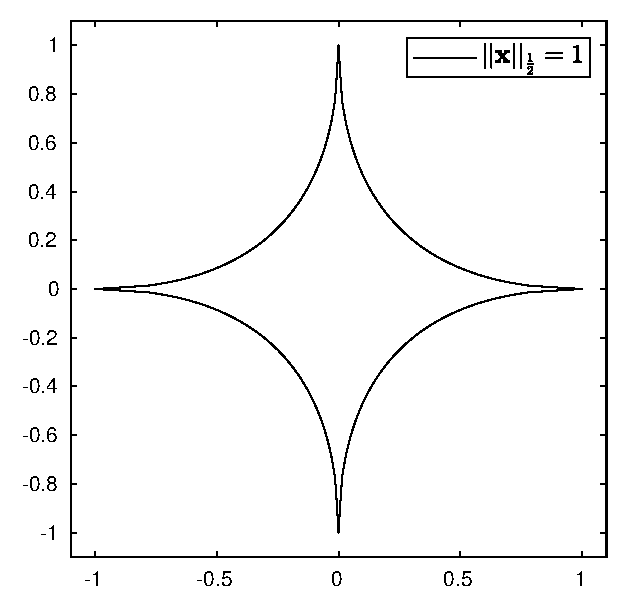
\includegraphics[width=0.6\linewidth]{eps/UnitBallNorm05}
  \captionof{figure}{$\left(\mathbb{R}^n, \|\cdot\|_p\right)$
    with $p\in(0,1)$ is not a normed space. 
  }
  \label{fig:notANormIfpLessThan1}
\end{Figure}

\begin{defn}
  \label{def:normsOfContFuncs}
  Let $\Omega\subset \mathbb{R}^n$ be a bounded open set.
  The \emph{$p$-norm of a continuous scalar function} in the linear space
  ${\cal C}(\overline{\Omega})$
  is 
  \begin{equation}
    \label{eq:pNormOfContFuncs}
    \forall v\in {\cal C}(\overline{\Omega}),\quad
    \|v\|_p :=  \left[\int_{\Omega}|v(\mathbf{x})|^p
      \dif \mathbf{x}\right]^{\frac{1}{p}}
  \end{equation}
  and the \emph{$\infty$-norm} or \emph{maximum norm}
  is given by 
  \begin{equation}
    \label{eq:maxNormOfContFuncs}
    \forall v\in {\cal C}(\overline{\Omega}),\quad
    \|v\|_{\infty} :=  \max_{\mathbf{x}\in \overline{\Omega}}
    |v(\mathbf{x})|.
  \end{equation}
\end{defn}

\begin{exm}
  $({\cal C}(\overline{\Omega}), \|\cdot\|_{\infty})$
  in Definition \ref{def:normsOfContFuncs} 
  is a normed space,
  so is $({\cal C}(\overline{\Omega}), \|\cdot\|_{p})$
  for any $p\in [1,\infty)$.
\end{exm}

\begin{exm}
  For the $\ell^{\infty}$ sequence space in (\ref{eq:ellInftySpace}), 
  \begin{displaymath}
    \ell^{\infty} := \left\{
      (a_n)_{n\in \mathbb{N}}: \sup_{n\in \mathbb{N}}|a_n| < \infty.
    \right\},
  \end{displaymath}
  define $\|\cdot\|_{\infty}: \ell^{\infty}\rightarrow \mathbb{R}^+\cup\{0\}$ as
  \begin{equation}
    \label{eq:ellInftyNorm}
    \left\|(a_n)_{n\in \mathbb{N}}\right\|_{\infty}
    = \sup_{n\in \mathbb{N}} |a_n|.
  \end{equation}
  Then $(\ell^{\infty}, \|\cdot\|_{\infty})$
  is a normed space.
\end{exm}

\begin{exm}
  For the $\ell^{p}$ space in (\ref{eq:lpSpace})
  with $p\in [1,\infty)$,
  \begin{displaymath}
    \ell^p := \left\{
      (a_n)_{n\in \mathbb{N}}: a_n\in \mathbb{C};
      \sum_{n\in \mathbb{N}} |a_n|^p < \infty
    \right\}, 
  \end{displaymath}
  we have
  \begin{align*}
     &\left\{
    \begin{array}{l}
      (a_n)_{n\in \mathbb{N}}\in \ell^p, \  
      (b_n)_{n\in \mathbb{N}}\in \ell^p
    \\
      |a+b|^p \le (|a|+|b|)^p \le 2^p(\max(|a|,|b|))^p
                  \le 2^p(|a|^p+|b|^p)
    \end{array}
    \right.
    \\
    &\Rightarrow
     (a_n)_{n\in \mathbb{N}}+(b_n)_{n\in \mathbb{N}}\in \ell^p,
  \end{align*}
  where the comparison test is applied.

  Then $(\ell^{p}, \|\cdot\|_{p})$
  is a normed space where
  \begin{equation}
    \label{eq:ellPNorm}
    \left\|(a_n)_{n\in \mathbb{N}^+}\right\|_p
    := \left(\sum_{n=1}^{\infty} |a_n|^p\right)^{\frac{1}{p}}.
  \end{equation}
\end{exm}

\subsection{Continuous maps of normed spaces}

\begin{lem}
  \label{lem:normIsContinuousMap}
  The norm function $\|\cdot\|$ is continuous.
\end{lem}

\begin{lem}
  \label{lem:monotonicityOfEuclideanNorm}
  The Euclidean norm $\|\cdot\|_p$
  in Example \ref{exm:RdEuclideanSpace}
  satisfies a monotonicity property:
  \begin{equation}
    \label{eq:monotonicityOfEuclideanNorm}
    1\le p \le q \le \infty
    \ \Rightarrow\
    \forall \mathbf{x}\in \mathbb{R}^n\ 
    \|\mathbf{x}\|_q \le \|\mathbf{x}\|_p.
  \end{equation}
\end{lem}

\begin{exm}
  The map $S: ({\cal C}[0,1], \|\cdot\|_{\infty}) \rightarrow
  (\mathbb{R}, |\cdot|)$,  
  \begin{equation}
    \label{eq:contFunExmpInt}
    S(f) = \int_0^1 f^2(x) \dif x, 
  \end{equation}
  is continuous.
  Indeed, for any $g\in {\cal C}[0,1]$, 
  we have
  \begin{align*}
    |S(f)-S(g)| &= 
    \left| \int_0^1 f^2(x) \dif x - \int_0^1 g^2(x) \dif x
                  \right|
    \\ &\le
         \int_0^1 \left|f(x)-g(x)\right|
                  \left|f(x)-g(x)+2g(x)\right|
         \dif x 
    \\ &\le
         \int_0^1 \left\|f-g\right\|_{\infty}
         \left(\left\|f-g\right\|_{\infty}+2\|g\|_{\infty}\right)
         \dif x, 
  \end{align*}
  which yields  
  \begin{align*}
    &\forall \epsilon>0,
    \exists \delta=\min\left(1,\frac{\epsilon}{1+2\|g\|_{\infty}}\right)
      \text{ s.t. }
    \|f-g\|_{\infty} < \delta\ \Rightarrow\
    \\
    & \left\|f-g\right\|_{\infty}
      \left(\left\|f-g\right\|_{\infty}+2\|g\|_{\infty}\right)
      <
      \left\|f-g\right\|_{\infty}
      \left(1+2\|g\|_{\infty}\right)
      < \epsilon
    \\
    & \Rightarrow\ |S(f)-S(g)| <\epsilon.
  \end{align*}
\end{exm}

\begin{exc}
  For $V={\cal C}[0,1]$ and $x_0\in [0,1]$,
  define $\ell_{x_0}: V\rightarrow \mathbb{R}$ as
  $\ell_{x_0}(v) := v(x_0)$.
  Show that $\ell_{x_0}$ is continuous on ${\cal C}[0,1]$.
\end{exc}

\begin{exm}
  \label{exm:continuityOfDifferentiation}
  The differentiation map
  \begin{displaymath}
    \frac{\dif}{\dif t}:
    ({\cal C}^1[a,b],\|\cdot\|_{\infty})
    \rightarrow ({\cal C}[a,b], \|\cdot\|_{\infty})
  \end{displaymath}
  is not continuous, but can be made
  continuous if we change the norm on ${\cal C}^1[a,b]$ to
  \begin{equation}
    \label{eq:normForC1}
    \|f\|_{1,\infty}:= \|f\|_{\infty} + \|f'\|_{\infty}.
  \end{equation}
  Indeed,
  for $f_n(t) = \frac{1}{\sqrt{n}}\cos(2\pi nt)$,
  we have
  \begin{align*}
    \forall n\in \mathbb{N}^+,\quad
    \|f'_n-\mathbf{0}'\|_{\infty} = 2\pi\sqrt{n} > 1, 
  \end{align*}
  yet $\|f_n-\mathbf{0}\|$ can be made arbitrarily small
  as $n \rightarrow \infty$.
  In contrast,
  $D: ({\cal C}^1[a,b],\|\cdot\|_{1,\infty})
  \rightarrow ({\cal C}[a,b], \|\cdot\|_{\infty})$ is continuous because
  \begin{align*}
    &\forall \epsilon>0,\ \exists \delta=\epsilon, \text{ s.t. }\ 
      \forall f,g\in {\cal C}^1[0,1],\ 
      \|f - g\|_{1,\infty}<\delta
    \ \Rightarrow\ 
    \\
    &
    \|Df - Dg\|_{\infty}
    = \|f' - g'\|_{\infty} \le
    \|f - g\|_{1,\infty} < \delta=\epsilon.
  \end{align*}
\end{exm}

\begin{exc}
  \label{exc:arcLengthFunctionNotContinuous}
  Show that the arc length function $L: {\cal C}^1[0,1]\rightarrow\mathbb{R}$,
  \begin{equation}
    \label{eq:arcLengthFunction}
    L(f) := \int_0^1 \sqrt{1+(f'(t))^2} \dif t,
  \end{equation}
  is not continuous if the norm of ${\cal C}^1[0,1]$ is
  $\|\cdot\|_{\infty}$,
  whereas it is continuous if we equip ${\cal C}^1[0,1]$ with
  (\ref{eq:normForC1}).
\end{exc}

\begin{exc}
  Is the function
  $S: (c_{00}, \|\cdot\|_{\infty}) \rightarrow (\mathbb{R}, |\cdot|)$,
  \begin{equation}
    \label{eq:c00FuncNotCont}
    S\left((a_n)_{n\in \mathbb{N}}\right) = \sum_{n=1}^{\infty} a_n^2
  \end{equation}
  continuous?
  Here $c_{00}$ is defined in Notation \ref{ntn:zeroSequenceSpaces}. 
\end{exc}

\subsection{Norm equivalence}
\label{sec:norm-equivalence}

\begin{defn}
  \label{def:equivalentNorms}
  Two norms $\|\cdot\|_A$ and $\|\cdot\|_B$ on $V$ are
  \emph{equivalent}, written $\|\cdot\|_A\sim \|\cdot\|_B$, iff
  \begin{equation}
    \label{eq:equivalentNorms}
    \exists c_1, c_2\in \mathbb{R}^+ \text{ s.t. }
    \forall v\in V,\quad
    c_1\|v\|_A \le \|v\|_B \le c_2 \|v\|_A.
  \end{equation}
\end{defn}

\begin{exm}
  The Euclidean norms in Definition \ref{def:EuclideanLpNorm}
  satisfy
  \begin{equation}
    \label{eq:EuclideanNormsAreEquivalent}
    \forall \mathbf{x} \in \mathbb{R}^n,\quad
    \|\mathbf{x}\|_{\infty} \le \|\mathbf{x}\|_p
    \le \sqrt[p]{n} \|\mathbf{x}\|_{\infty}.
  \end{equation}
  Therefore all the Euclidean $\ell_p$ norms
  are equivalent.
\end{exm}

\begin{exm}
  The operator norm and the Hilbert-Schmidt norm
  in Definitions \ref{def:operatorNorm}
  and \ref{def:HilbertSchmidtNorm}
  are equivalent. 
\end{exm}

\begin{exc}
  \label{exc:equivalenceOfNorms}
  Show that $\sim$ in Definition \ref{def:equivalentNorms}
  defines an equivalence relation
  on the set of all norms on $V$.
\end{exc}

\begin{lem}
  \label{lem:normEquivCondViaConvergence}
  Show that two norms $\|\cdot\|_A$ and $\|\cdot\|_B$
  on a linear space $V$ are equivalent
  if and only if each sequence converging with respect to
  $\|\cdot\|_A$
  also converges with respect to $\|\cdot\|_B$.
\end{lem}

\begin{thm}
  \label{thm:normEquivalenceRn}
  All norms are equivalent on $\mathbb{R}^n$ or $\mathbb{C}^n$.
\end{thm}

\begin{coro}
  \label{coro:normEquivalenceFiniteDim}
  Over a finite-dimensional space,
  any two norms are equivalent.
\end{coro}

\begin{exm}
  In the normed space $V:= {\cal C}[0,1]$, 
  consider a sequence of functions
  $(u_n)$ given by
  \begin{displaymath}
    u_n(x) :=
    \begin{cases}
      1-nx, & x\in [0,\frac{1}{n}];
      \\
      0, & x\in (\frac{1}{n}, 1].
    \end{cases}
  \end{displaymath}
  For the $p$-norm in (\ref{eq:pNormOfContFuncs}),
  we have $\|u_n\|_p = [n(p+1)]^{-\frac{1}{p}}$
  and thus the sequence $(u_n)$ converges
  to $u=0$ in $(V,\|\cdot\|_p)$.
  However, for the $\infty$-norm in (\ref{eq:maxNormOfContFuncs}),
  we have $\|u_n\|_{\infty} = 1$.
  By Definition \ref{def:equivalentNorms}, 
  these two norms can not be equivalent. 
\end{exm}

\subsection{Completeness}

\begin{defn}[Banach spaces]
  \label{def:BanachSpace}  
  A \emph{Banach space} is a \emph{complete} normed space, 
  i.e., a normed space $V$ such that
  every Cauchy sequence in $V$ converges in $V$.
\end{defn}

\begin{defn}
  A \emph{Hilbert space} is a Banach space equipped with an inner product.
\end{defn}

\begin{thm}
  \label{thm:contFuncWithInftyNormIsComplete}
  $\left({\cal C}[a,b], \|\cdot\|_{\infty}\right)$
  is a Banach space.
\end{thm}

\begin{exm}
  \label{exm:CpIsNotComplete}
  For $p\in[1,\infty)$, 
  the space $\left({\cal C}(\overline{\Omega}), \|\cdot\|_{p}\right)$
  is not a Banach space. 
  Consider % $\Omega=[0,1]$ and
  $\left(u_n\right)_{n\in \mathbb{N}}\subset
  {\cal C}[0,1]$
  given by
  \begin{equation}
    \label{eq:CpIsNotComplete}
    u_n(x) =
    \begin{cases}
      0, & x\in [0,\frac{1}{2}-\frac{1}{2n}];
      \\
      nx - \frac{n-1}{2}, & x\in [\frac{1}{2}-\frac{1}{2n},
      \frac{1}{2}+\frac{1}{2n}];
      \\
      1 & x\in [\frac{1}{2}+\frac{1}{2n},1].
    \end{cases}
  \end{equation}
  $(u_n)_{n\in \mathbb{N}}$ is clearly Cauchy
  and we have
  \begin{displaymath}
    \lim_{n\rightarrow \infty} u_n = u(x) =
    \begin{cases}
      0, & x\in [0, \frac{1}{2});
      \\
      1, & x\in (\frac{1}{2}, 1].
    \end{cases}
  \end{displaymath}
  But $u(x)$ cannot be in ${\cal C}(\overline{\Omega})$
  no matter how we define $u(\frac{1}{2})$.
\end{exm}

\begin{defn}
  \label{def:isomorphicN0ormedSpaces}
  Two normed spaces $X$ and $Y$
  are \emph{isomorphic}, written $X\simeq Y$, 
  iff there exists a bijective linear map
  $T\in {\cal L}(X, Y)$ such that
  \begin{equation}
    \label{eq:isometricIsomorphism}
    \forall v\in X,\quad \|T v\|_Y = \|v\|_X.
  \end{equation}
  Then $T$ is an \emph{(isometric) isomorphism}
  between $X$ and $Y$.
\end{defn}

\begin{thm}
  \label{thm:completionOfNormedSpace}
  Every normed space $V$ has a unique \emph{completion}
  up to isometric isomorphism,
  i.e., 
  there exists a unique Banach space $W$
  such that $V$ is isomorphic to a dense subspace of $W$.
\end{thm}

\begin{defn}
  \label{def:completionOfNormedSpace}
  The Banach space $W$ in Theorem \ref{thm:completionOfNormedSpace}
  is called the \emph{completion of the normed space} $V$.  
\end{defn}

\begin{exc}
  Show that the sequence space
  $(\ell^p, \|\cdot\|_p)$ is complete
  for $p\in[1,+\infty]$.
\end{exc}

\begin{exc}
  Define ${\cal C}_b[0,\infty)$ as the set of all functions
  $f$ that are continuous on $[0,\infty)$
  and satisfy
  \begin{displaymath}
    \|f\|_{\infty} := \sup_{x\ge 0}|f(x)| < \infty.
  \end{displaymath}
  Show ${\cal C}_b[0,\infty)$ with this norm is complete.
\end{exc}

\begin{exc}
  Define ${\cal C}^{\alpha}[a,b]$ as the set of all functions
  $f\in {\cal C}[a,b]$ satisfying
  \begin{displaymath}
    M_{\alpha}(f) := \sup_{x,y\in[a,b]; x\ne y}
    \frac{|f(x)-f(y)|}{|x-y|^{\alpha}} < \infty.
  \end{displaymath}
  Define $\|f\|_{\alpha} = \|f\|_{\infty}+M_{\alpha}(f)$.
  Show that $({\cal C}^{\alpha}[a,b], \|\cdot\|_{\alpha})$
  is a Banach space.
\end{exc}

\subsection{Convergence of function series}

\begin{thm}
  \label{thm:absolutelyConvergentSeriesConvergeInBanach}
  In a Banach space, absolutely convergent series converge.
  More precisely,
  if $(x_n)_{n\in \mathbb{N}}$ is a sequence
  in a Banach space $(X, \|\cdot\|)$
  such that $\sum_{n=1}^{\infty} \|x_n\|$ converges,
  then $\sum_{n=1}^{\infty} x_n$ converges in $X$.
  Furthermore,
  \begin{equation}
    \label{eq:triangleInequalityInfty}
    \left\|\sum_{n=1}^{\infty}x_n\right\|
    \le \sum_{n=1}^{\infty} \left\|x_n\right\|.
  \end{equation}
\end{thm}

\begin{exm}
  The series $\sum_{n=1}^{\infty}\frac{1}{n^2}\sin(nx)$
  converges in $({\cal C}[0,2 \pi], \|\cdot\|_{\infty})$
  since $\sum_{n=1}^{\infty}\frac{1}{n^2}$ converges in $\mathbb{R}$.
  Hence $x\mapsto \sum_{n=1}^{\infty}\frac{1}{n^2}\sin(nx)$
  defines a continuous function. 
\end{exm}

\begin{exc}
  Prove the converse of Theorem
  \ref{thm:absolutelyConvergentSeriesConvergeInBanach},
  i.e., a normed space $X$ is complete
  if every absolutely convergent series converges in $X$.
\end{exc}

\begin{thm}[Weierstrass M-test]
  \label{thm:WeierstrassMtest}
  Suppose a sequence of functions $(f_n)_{n=1}^{\infty}$ 
  defined on a complete normed space ${\cal X}$ satisfies
  \begin{equation}
    \label{eq:WeierstrassMtest}
    \forall x\in{\cal X},\ \ \|f_n(x)\|\le M_n.
  \end{equation}
  Then the convergence of $\sum_{i=1}^n M_i$ 
  implies the uniform convergence of the series $\sum_{i=1}^n f_i$ 
  to some  $f\in{\cal X}$.
\end{thm}

\begin{exc}
  Prove Theorem \ref{thm:WeierstrassMtest}
  via Theorem \ref{thm:CauchyCriterionUniformConv}. 
\end{exc}

\section{The space ${\cal CL}(X,Y)$}
\label{sec:space-CLXY}

\begin{defn}
  \label{def:boundedLinearMap}
  A linear map $T\in {\cal L}(X,Y)$ is \emph{bounded} if
  it maps any bounded set in ${\cal X}$
  to a bounded set in ${\cal Y}$, i.e., 
  \begin{equation}
    \label{eq:boundedLinearMap}
    \exists M\in \mathbb{R}^+ \text{ s.t. }
    \forall x\in X,\ \  \|Tx\|_Y\le M \|x\|_X.
  \end{equation}
\end{defn}

\begin{ntn}
  ${\cal C}{\cal L}(X,Y)$ denotes
  the \emph{set of all continuous linear transformations
  or bounded linear transformations}
  from the normed space $X$ to the normed space $Y$,
  \begin{equation}
    \label{eq:CL-XY}
    {\cal CL}(X,Y) := {\cal C}(X,Y) \cap {\cal L}(X,Y),
  \end{equation}
  where ${\cal L}(X,Y)$ is given by Notation \ref{ntn:spaceOfLinearMaps}.
  We also write ${\cal CL}(X)$ if $Y=X$, 
\end{ntn}

\subsection{Boundedness = continuity}

\begin{thm}
  \label{thm:contLinearOpEquBoundedOp}
  For any map $T\in {\cal L}(X,Y)$, the following statements are equivalent:
  \begin{enumerate}[(a)]\itemsep0em
  \item $T$ is continuous,
  \item $T$ is continuous at $\mathbf{0}$,
  \item $T$ is bounded. 
  \end{enumerate}
\end{thm}

\begin{exm}
  \label{exm:leftAndRightShiftOnEll2}
  The left shift operator $L: \ell^2\rightarrow \ell^2$
  and right shift operator $R: \ell^2\rightarrow \ell^2$,
  \begin{align}
    \label{eq:leftShift}
    L(a_1, a_2, a_3, \ldots) &= (a_2, a_3, \ldots),
    \\
    \label{eq:rightShift}
    R(a_1, a_2, a_3, \ldots) &= (0, a_1, a_2,  \ldots),
  \end{align}
  are linear operators.
  Furthermore, $L, R\in {\cal CL}(\ell^2)$ because
  they are bounded:
  \begin{displaymath}
    \|L(a_n)_{n\in \mathbb{N}}\| \le \|(a_n)_{n\in \mathbb{N}}\|,
    \quad
    \|R(a_n)_{n\in \mathbb{N}}\| = \|(a_n)_{n\in \mathbb{N}}\|.
  \end{displaymath}
\end{exm}

\begin{exm}
  \label{exm:integralAsCLmap}
  The linear map $T: ({\cal C}[a,b],\|\cdot\|_{\infty})\rightarrow
  \mathbb{R}$
  given by $T(f) = \int_a^b f(t) \dif t$ is continuous
  because
  \begin{displaymath}
    |T(f)| = \left|\int_a^b f(t) \dif t\right|
    \le \int_a^b\|f\|_{\infty}\dif t
    = (b-a) \|f\|_{\infty}.
  \end{displaymath}
  By Definition \ref{def:continuousFuncPointMetricSpace}, 
  $T$ preserves convergent sequences:
  \begin{displaymath}
    \lim_{n\rightarrow \infty} f_n = f
    \ \Rightarrow\
    \lim_{n\rightarrow \infty} \int_a^b f_n = \int_a^b f.
  \end{displaymath}
  In other words, the continuity of $T$
  under $\|\cdot\|_{\infty}$ guarantees
  that $T$ and $\lim_{n\rightarrow \infty}$ are commutative;
  see Section \ref{sec:uniform-convergence}.
\end{exm}

\begin{exm}
  The continuity of differentiation maps in Example
  \ref{exm:continuityOfDifferentiation}
  can be determined by Theorem \ref{thm:contLinearOpEquBoundedOp}.
  For $\|\cdot\|_{1,\infty}$,
  we have $\|D \mathbf{x}\|_{\infty} \le \|\mathbf{x}\|_{1,\infty}$, 
  and thus the operator $D: \left({\cal C}[0,1],\|\cdot\|_{1,\infty}\right)
  \rightarrow \left({\cal C}[0,1],\|\cdot\|_{\infty}\right)$
  is continuous.
  
  In comparison,
  $D: \left({\cal C}[0,1],\|\cdot\|_{\infty}\right)
  \rightarrow \left({\cal C}[0,1],\|\cdot\|_{\infty}\right)$
  is not continuous: 
  for $\mathbf{x}_n=t^n$, we have $\|x_n\|_{\infty}=1$ yet 
  $\lim_{n\rightarrow \infty} \|\mathbf{x}_n'\|_{\infty} = \infty$.
\end{exm}

\begin{coro}
  \label{coro:CLXYisSubspaceOfLXY}
  ${\cal CL}(X,Y)$ is a subspace of ${\cal L}(X,Y)$.
\end{coro}

\begin{coro}
  \label{coro:finiteDimCLXYisLXY}
  For finite-dimensional normed spaces $X$ and $Y$,
  we have ${\cal L}(X,Y)={\cal CL}(X,Y)$.
\end{coro}

\begin{exc}
  For an infinite-dimensional matrix $A$ satisfying
  $\sum_{i=1}^{\infty}\sum_{j=1}^{\infty}a_{ij}^2<\infty$,
  define $T_A: \ell^2\rightarrow \ell^2$
  by
  \begin{equation}
    \label{eq:inftMatrixL2}
    \forall \mathbf{x}=(x_j)_{j\in \mathbb{N}}\in \ell^2,\quad
    T_A \mathbf{x} = A \mathbf{x} =
    \left(\sum_{j=1}^{\infty} a_{ij}x_j \right)_{i\in \mathbb{N}^+}.
  \end{equation}
  Prove $T_A\in {\cal CL}(\ell^2)$.
\end{exc}

\begin{exc}
  For $A,B\in {\cal C}[a,b]$ and
  \begin{equation}
    \label{eq:C10}
    S := \{f\in {\cal C}^1[a,b]: f(a)=f(b)=0\}, 
  \end{equation}
  show that the map 
  $L: (S, \|\cdot\|_{1,\infty}) \rightarrow \mathbb{R}$
  given by
  \begin{displaymath}
    L(f) = \int_a^b \bigl[A(t)f(t)+B(t)f'(t)\bigr] \dif t
  \end{displaymath}
  is a bounded linear transformation.
\end{exc}

\subsection{Consequences on the topology}

\begin{ntn}
  \label{ntn:setLinearOpNotation}
  For a vector space $X$ and 
  its subsets $A$, $A_1$, $A_2$, 
  we write
    \begin{equation}
    \label{eq:setLinearOpNotation}
      \begin{array}{rl}
        \forall \alpha\in \mathbb{R},
        \quad \alpha A &:= \{\alpha a, a\in A\};
        \\
        \forall w\in X,\quad 
        A + w &:= \{a+w, a\in A\}.
        \\
        \forall A_1, A_2 \subset X,\quad 
        A_1 + A_2 &:= \{a_1+a_2: a_1\in A_1, a_2\in A_2\}.
      \end{array}
  \end{equation}
\end{ntn}

\begin{lem}
  \label{lem:KernelIsClosed}
  The null space of any linear map $A\in \mathbb{R}^{m\times n}$
  is closed in $\mathbb{R}^n$.
\end{lem}

\begin{thm}
  \label{thm:finiteDimSubspaceIsClosed}
  Every subspace of $\mathbb{R}^n$ is closed.
\end{thm}

\begin{lem}
  \label{lem:openMapCharInNormedSpaces}
  Let $X$ and $Y$ be normed spaces.
  A bounded linear map $T\in {\cal CL}(X,Y)$ is open
  in the sense of Definition \ref{def:openMap}
  if and only if the image of the unit open ball in $X$ under $T$
  contains some open ball centered at $\mathbf{0}_Y$ in $Y$, i.e.,
  \begin{equation}
    \label{eq:openMapCharInNormedSpaces}
    \exists \delta>0 \text{ s.t. }
    B(\mathbf{0}_Y, \delta) \subset T\left({B(\mathbf{0}_X,1)}\right).
  \end{equation}
\end{lem}

\begin{thm}[Baire]
  \label{thm:Baire}
  Suppose $(F_n)_{n\in \mathbb{N}}$ is a sequence of closed sets
  in a Banach space $X$ such that $X=\cup_{n\in \mathbb{N}} F_n$.
  Then there exists $n\in \mathbb{N}$
  and a nonempty open set $U$ such that $U\subset F_n$.
\end{thm}

\begin{lem}[Unit open ball]
  \label{lem:helpForOpenMapping}
  Suppose $X$ and $Y$ are Banach spaces
  and $T\in {\cal CL}(X,Y)$ is surjective.
  Then the image $T(B_0)$ of the open ball
  $B_0:=B(\mathbf{0}_X,1)$ contains an open ball about $\mathbf{0}_Y$.
\end{lem}

\begin{thm}[Open mapping]
  \label{thm:openMapping}
  For Banach spaces $X$ and $Y$,
  any surjective map $T\in {\cal CL}(X,Y)$ is open.
\end{thm}

\begin{exm}
  The following function $f: \mathbb{R}\rightarrow \mathbb{R}$, 
  \begin{displaymath}
    f(x) =
    \begin{cases}
      x+1 & \text{if } x\in (-\infty, -1];
      \\
      0 & \text{if } x\in (-1, +1);
      \\
      x-1 & \text{if } x\in [+1,+\infty),
    \end{cases}
  \end{displaymath}
  is surjective and continuous;
  but since $f((-1,1))=\{0\}$ is closed,
  $f$ is not open.
  By the open mapping theorem,
  if a map between two Banach spaces
  is not open but surjective and continuous, 
  then it must be nonlinear.
\end{exm}

\subsection{Operator norms}
\label{sec:operator-norms}

\begin{lem}
  \label{def:OpNormCLXY}
  The \emph{operator norm}
  $\|\cdot\|: {\cal CL}(X,Y)\rightarrow \mathbb{R}$
  of an operator $T\in {\cal CL}(X,Y)$ given by 
  \begin{equation}
    \label{eq:OpNormCLXY}
    \|T\|= \sup S \text{ where }
    S:=\bigl\{\|Tx\|: x\in X, \|x\|\le 1\bigr\} 
  \end{equation}
  is well defined, i.e., $\|T\|$ is a unique bounded real number.
\end{lem}

\begin{lem}
  \label{lem:opNormIsLeastUpperBound}
  Any $T\in {\cal CL}(X,Y)$ satisfies 
  \begin{equation}
    \label{eq:opNormIsLeastUpperBound}
    \left(\forall x\in X, \|Tx\|\le M \|x\|\right)
    \ \Rightarrow\ \|T\|\le M.
  \end{equation}
\end{lem}

\begin{lem}
  \label{lem:TxNormLE-Tnorm-xnorm}
  $\forall T\in {\cal CL}(X,Y)$, $\forall x\in X$,
  $\|Tx\|\le \|T\|\|x\|$.
\end{lem}

\begin{lem}
  \label{lem:STNormLE-SnormTnorm}
  $\forall S\in {\cal CL}(X,Y)$,
  $\forall T\in {\cal CL}(Y,Z)$, 
  we have $\|ST\|\le \|S\|\|T\|$.
\end{lem}

\begin{thm}
  \label{thm:OpNormCLXY}
  $\bigl({\cal CL}(X,Y), \|\cdot\|\bigr)$ is a normed space.
\end{thm}

\begin{lem}
  \label{lem:YisBanachImpliesCLXYisBanach}
  For a normed space $X$,
  the normed space \mbox{$\bigl({\cal CL}(X,Y), \|\cdot\|\bigr)$} is complete
  if and only if $Y$ is a Banach space.
\end{lem}

\begin{coro}
  If $X$ is a normed space over $\mathbb{R}$,
  then the dual space of $X$, $X'={\cal CL}(X,\mathbb{R})$,
  is a Banach space with the operator norm.
\end{coro}

\begin{coro}
  \label{coro:XisBanachSoIsCLX}
  If $X$ is a Banach space,
  then ${\cal CL}(X)$ is a Banach space with the operator norm.
\end{coro}

\begin{defn}
  A \emph{normed algebra} is an algebra $V$ (as in Definition \ref{def:algebra})
  with a norm $\|\cdot\|$ satisfying
  \begin{equation}
    \label{eq:normedAlgebra}
    \forall u,v \in V,\quad \|uv\|\le \|u\|\|v\|.
  \end{equation}
  A \emph{Banach algebra} is a normed algebra that is complete.
\end{defn}

\subsection{Invertible operators}
\label{sec:invertible-operators}

\begin{lem}
  In a finite-dimensional vector space $X$, 
  if two operators $T,S\in {\cal L}(X)$ satisfy
  $TS = I$, then $ST = I$.
\end{lem}

\begin{exm}
  For the shift operators on $\ell^2$
  in Example \ref{exm:leftAndRightShiftOnEll2},
  we have $LR=I$ but $RL\ne I$,
  \begin{displaymath}
    RL(1,0,0,\ldots) = (0,0,0,\ldots).
  \end{displaymath}
\end{exm}

\begin{defn}
  \label{def:invertibleOps}
  For vector spaces $X$ and $Y$,
  a linear map \mbox{$A\in {\cal L}(X,Y)$} is \emph{invertible}
  if there exists $B\in {\cal L}(Y,X)$
  such that $AB=I\in {\cal L}(Y)$
  and $BA=I\in {\cal L}(X)$. 
  Then $B$ is called the \emph{inverse} of $A$.
\end{defn}

\begin{exc}
  Prove that the inverse of $A\in {\cal L}(X,Y)$ is unique
  if $A$ is invertible.
\end{exc}

\begin{lem}
  \label{lem:invertibleImpliesBijective}
  For any vector spaces $X$ and $Y$, 
  if a linear map $A\in {\cal L}(X,Y)$ is invertible, 
  then $A$ is bijective.
\end{lem}

\begin{lem}
  \label{lem:invertibleCLmapIsLinear}
  For two vectors spaces $X$ and $Y$, 
  if a map $A\in {\cal L}(X,Y)$ is invertible,
  then its inverse $A^{-1}$ is linear.
\end{lem}

\begin{lem}
  \label{lem:bijectiveImpliesInvertibleFiniteDim}
  For two finite-dimensional vector spaces $X$ and $Y$, 
  a linear map $A\in {\cal L}(X,Y)$ is invertible
  provided that it is bijective.
\end{lem}

\begin{thm}
  For finite-dimensional normed spaces $X$ and $Y$,
  a linear map $A\in {\cal CL}(X,Y)$ is invertible
  if and only if $A$ is bijective,
  in which case we also have $A^{-1}\in {\cal CL}(Y,X)$. 
\end{thm}

\begin{exm}
  \label{exm:bijectiveButNotInvertible}
  The map $A: c_{00}\rightarrow c_{00}$ given by
  \begin{displaymath}
    \forall (x_n)_{n\in \mathbb{N}} \in c_{00},\quad
    A(x_1, x_2, x_3, \ldots) = (x_1, \frac{x_2}{2}, \frac{x_3}{3}, \ldots)
  \end{displaymath}
  is linear, bijective, and continuous
  (since $\|A\mathbf{x}\|_{\infty}\le \|\mathbf{x}\|_{\infty}$).
  However, it is not invertible in ${\cal CL}(c_{00})$.
  Suppose it is and $B\in{\cal CL}(c_{00})$ is the inverse of $A$.
  Then for the sequences $\mathbf{e}_m:=(0,\ldots,0,1,0,\ldots)$
  where all terms are 0 except that the $m$th term is 1,
  we have
  \begin{displaymath}
    1 = \|\mathbf{e}_m\|_{\infty}
    = \|BA\mathbf{e}_m\|_{\infty}
    \le \|B\|\|A\mathbf{e}_m\|_{\infty}= \frac{\|B\|}{m}.
  \end{displaymath}
  Hence $\forall m\in \mathbb{N}$, $\|B\|\ge m$
  and this contradicts Lemma \ref{def:OpNormCLXY}.
\end{exm}

\begin{thm}[Banach]
  \label{thm:bijectiveCLmapBetweenBanachSpacesIsInvertible}
  For Banach spaces $X$ and $Y$, 
  a map $T\in {\cal CL}(X,Y)$
  is invertible with $T^{-1}\in {\cal CL}(Y,X)$
  if and only if $T$ is bijective.
\end{thm}

\begin{thm}[Closed graph]
  \label{thm:closedGraph}
  For two Banach spaces $(X,\|\cdot\|_X)$ and $(Y,\|\cdot\|_Y)$,
  a map $T\in {\cal L}(X,Y)$ is continuous
  if and only if its graph ${\cal G}(T) := \{(x,Tx): x\in X\}$
  is closed
  in $(X\times Y, \|\cdot\|_{\infty})$
  where 
  \begin{equation}
    \label{eq:productInftyNorm}
    \forall (x,y)\in X\times Y,\quad
    \|(x,y)\|_{\infty}:=\max(\|x\|_X,\|y\|_Y).
  \end{equation}
\end{thm}

\subsection{Neumann series}
\label{sec:series-operators}

\begin{thm}[Neumann series]
  \label{thm:NeumannSeries}
  Suppose $X$ is a Banach space
  and $A\in {\cal CL}(X)$ has $\|A\|<1$.
  Then we have
  \begin{enumerate}[(NST-1)]\itemsep0em
  \item $I-A$ is invertible in ${\cal CL}(X)$,
  \item $(I-A)^{-1}=I + A + \cdots + A^n +\cdots
    = \sum_{n=0}^{\infty} A^n$, 
  \item $\left\|(I-A)^{-1}\right\| \le \frac{1}{1-\|A\|}$.
  \end{enumerate}
\end{thm}

\begin{thm}
  \label{thm:expOfOpCLX}
  Suppose $X$ is a Banach space. 
  Then the exponential of $A\in {\cal CL}(X)$,
  defined as
  \begin{equation}
    \label{eq:expOfOpCLX}
    e^A := \sum_{n=0}^{\infty} \frac{1}{n!} A^n, 
  \end{equation}
  converges in ${\cal CL}(X)$.
\end{thm}

\begin{lem}
  \label{lem:expOfOpCLX-Dt}
  For a Banach space $X$, 
  $A\in {\cal CL}(X)$ satisfies
  \begin{equation}
    \label{eq:expOfOpCLX-Dt}
   \frac{\dif}{\dif t} e^{tA} = A e^{tA} = e^{tA}A.
  \end{equation}
\end{lem}

\begin{lem}
  \label{lem:expOfOpCLX-commute}
  For a Banach space $X$, 
  if $A,B\in {\cal CL}(X)$ commute,
  i.e. $AB=BA$, 
  then 
  \begin{equation}
    \label{eq:expOfOpCLX-commute}
    e^{A+B} = e^{A}e^B.
  \end{equation}
\end{lem}

\begin{coro}
  \label{coro:expOfOpCLX-inverse}
  For a Banach space $X$
  and $A\in {\cal CL}(X)$,
  $e^A$ is always invertible
  with its inverse as $e^{-A}$.  
\end{coro}

\begin{thm}[Existence and uniqueness of ODEs]
  \label{thm:scalarODE-Banach}
  For a Banach space $X$ and $A\in {\cal CL}(X)$,
  the IVP
  $\frac{\dif x}{\dif t}(t) = A x(t)$ 
  with initial condition $x(0)=x_0\in X$
  has a unique solution $x(t)= e^{tA}x_0$ for $t\in \mathbb{R}$.
\end{thm}

\subsection{Uniform boundedness}
\label{sec:uniform-boundedness}

\begin{lem}
  \label{lem:SymmetricAndConvexAndOpenSet}
  Suppose $X$ is a normed space and a subset $A\subset X$
  satisfies
  \begin{itemize}\itemsep0em
  \item $A$ is symmetric, i.e., $-A=A$;
  \item $A$ is mid-point convex, i.e.,
    $\forall x,y\in A$, $\frac{x+y}{2}\in A$,
  \item there exists a nonempty open set $U\subset A$.
  \end{itemize}
  Then there exists $\delta>0$ such that
  $B(\mathbf{0}_X,\delta)\subset A$.
\end{lem}

\begin{thm}[Principle of uniform boundedness]
  \label{thm:uniform-boundedness}
  Suppose $X$ is a Banach space and $Y$ is a normed space.
  For a family of maps $T_i\in {\cal CL}(X,Y)$, $i\in I$, 
  ``pointwise boundedness''
  implies ``uniform boundedness,'' % i.e., 
  \begin{displaymath}
    \forall x\in X,\quad
    \sup_{i\in I} \|T_i x\| < +\infty
    \ \Rightarrow\ 
    \sup_{i\in I} \|T_i\| <+\infty.
  \end{displaymath}
\end{thm}

\begin{exm}
  Many PDEs can be written in the form
  \begin{displaymath}
    Tx = y,
  \end{displaymath}
  where $y$ is a known vector incorporating initial and boundary
  conditions,
  $x$ is the unknown, 
  and $T$ is a continuous linear operator.
  If the PDE is well-posed, we can often assume
  that $T$ is a bijection,
  hence by Theorem
  \ref{thm:bijectiveCLmapBetweenBanachSpacesIsInvertible}
  the inverse of $T$ is a bounded linear operator
  and we write $x=T^{-1}y$.
  In numerically solving the PDE,
  we usually approximate $y$ by a grid function $y_n$ 
  and approximate $T^{-1}$ by a discrete operator $T^{-1}_n$.
  The convergence usually means
  \begin{displaymath}
    \forall y\in {\cal C}^r(\overline{\Omega}),
    \lim_{n\rightarrow \infty} y_n = y,\ 
    \lim_{n\rightarrow \infty} T^{-1}_n y_n = x, 
  \end{displaymath}
  i.e., $\sup_{n\rightarrow \infty} \|T^{-1}_n y_n\|<\infty$.
  Theorem \ref{thm:uniform-boundedness} then implies
  $\sup_{n\in \mathbb{N}}\|T_n^{-1}\|<\infty$,
  which usually implies some form of numerical stability.
\end{exm}

\begin{thm}[Banach-Steinhaus]
  \label{thm:Banach-Steinhauss}
  Suppose $X$ and $Y$ are Banach spaces.
  If a sequence $(T_n)_{n\in \mathbb{N}}\in {\cal CL}(X,Y)$
  has
  \begin{displaymath}
    \forall x\in X, \
    \lim_{n\rightarrow \infty} \|T_n x\| < \infty, 
  \end{displaymath}
  then the map $x\mapsto \lim_{n\rightarrow \infty} T_n x$
  belongs to ${\cal CL}(X,Y)$.
\end{thm}

%%% Local Variables:
%%% mode: latex
%%% TeX-master: "../numPDEs2cols"
%%% End:



\end{multicols}


\clearpage

\pagestyle{fancy}
\fancyhead{}
\lhead{}
\chead{Bibliography}
\rhead{\fYear}

\bibliography{bib/numericalAnalysis}
%\bibliographystyle{abbrv}
\bibliographystyle{abbrvnat}
\setcitestyle{authoryear,open={[},close={]}}

\printindex

\end{document}



%%% Local Variables: 
%%% mode: latex
%%% TeX-master: t
%%% End: 

% LocalWords:  FPN underflows denormalized FPNs matlab eps IEEE iff
% LocalWords:  cardinality significand quadratically bijection unary
%  LocalWords:  contractive bijective postcondition invertible arity
%  LocalWords:  subspaces surjective injective monomials additivity
%  LocalWords:  nullary Abelian abelian finitary eigenvectors adjoint
%  LocalWords:  eigenvector nullspace Hermitian unitarily multiset
%  LocalWords:  nonsingular nonconstant homomorphism homomorphisms
%  LocalWords:  isomorphically indeterminates subfield isomorphism
%  LocalWords:  nondefective diagonalizable contrapositive cofactor
%  LocalWords:  submatrix nilpotent positivity orthonormal extremum
%  LocalWords:  Jacobian nonsquare semidefinite nonnegative RHS LLS
%  LocalWords:  roundoff
